%************************************************
\chapter{Modelling hippocampal place cells for visual localization}\label{ch:chapter5} % 
%************************************************


\section{Introduction}

Animals use a variety of environmental cues in order to recognise their location.  One of the key behaviours found in a certain type of biological neuron -- known as place cells -- is a rate-coding effect: a neuron's rate of firing decreases with distance from some landmark location. In this chapter, we used visual information from wearable and hand-held cameras in order to reproduce this rate-coding effect in artificial place cells (APCs).  The accuracy of localisation using these APCs was evaluated using the different visual descriptors presented in chapter~\ref{ch:chapter4} and different place cell widths. Simple localisation using APCs was feasible by noting the identity of the APC yielding the maximum response. We also propose using joint coding within a number of automatically defined APCs as a population code for self-localisation. Using both approaches we were able to demonstrate good self-localisation from very small images taken in indoor settings. The error performance using APCs is favourable when compared with ground-truth and LSD-SLAM, even without the use of a motion model.

\subsection{Motivation}

This work explores the potential of location-sensitive computational units to achieve self-localisation by using the images from wearable or hand-held cameras.  Our approach is motivated by studies of biological vision which suggest that, in many species, multiple strategies are employed to help animals self-localise. Examples include the use of the visual horizon and path integration in ants~\cite{narendra2013mapping} and the use of optic flow in insects and birds \cite{krapp2000neuronal, bhagavatula2011optic}. Indeed, multiple computational approaches appear to be simultaneously at work even within a single species and for one sensing modality, such as vision. Such approaches can be successfully transferred from biology into computer vision; see for example, the combined use of optic flow and image descriptors that were suggested to mimic the visual homing system of insects~\cite{vardy2005biologically}.

Biological place cells display location-dependent firing. We describe how to mimic place cell behaviour from appearance information in order to provide localisation within an indoor environment. In terms of computer vision, our research question might be articulated as:

\begin{quotation}\textit{Given a video sequence taken by a person as they walk, can we generate artificial place cell responses that are able to localise that person with respect to previous journeys?
}\end{quotation}

\subsection{Summary of Contributions}

The approach to indoor localization described in this chapter is novel for several reasons.First, we suggest methods for appearance-based localisation by mimicking the behaviour of hippocampal place cells; the computational units of this behaviour -- Artificial Place Cells (APCs) -- are able to use distinctive information from image queries based on the recall of previously visited places. Secondly, we describe a complete pipeline of visual localisation that incorporates a decoder for the APC activity; this decoder takes the form of a Generalized Regression Neural Network (GRNN). Finally, we provide an evaluation of the proposed localisation method using a publicly available database of indoor sequences containing more than 120,000 frames and 3 km in length. Results suggest that sub-metre localisation error is achievable within this dataset. 


\section{Background}

Navigation is one of the more complex tasks performed by animals; it involves integration of multiple sensory inputs, combining past information (memory) and also the execution of physical actions to perform navigation movements.

John O'Keefe, together with Edvard and May-Britt Moser, received the Nobel Prize in Physiology or Medicine (2014) for their discovery and subsequent elucidation of place and, subsequently, grid cells in the brain, respectively. Their early findings suggested that navigation in the moving rat is based on a cognitive map of the environment; in this map, a set of landmarks is created, and the spatial relationship between these is used to navigate \cite{keefe1978hippocampus}. The implications  are interesting, partly for the potential importance in understanding some forms of dementia, but also because the cells encoding an organism's own spatial position are found in one of the less understood areas of mammalian brains: the hippocampus, with a key role in memory, and its adjacent brain areas. 

Humans, like other animals, need a sense of position to perform basic interaction with the environment. This interaction is often finding our way from one place to another and place awareness is integrated with distance and direction information to navigate. 


\subsection{Biological Place Cells (BPC)}


Place cells are special types of neurons located in the hippocampus which attain higher-than-average firing when an animal ``recognises'' a particular place in its environment. Grid cells, located next to the hippocampus in the entorhinal cortex, provide the brain with a reference system for navigation, a ``grid'' that is speculated to be used as a form of coordinate system for the creation of spatial maps. Although the existence of place and grid cells is without question, the computational description of what the cells do is debatable. However, the combination of place and grid cells within neural circuitry appears crucial for the execution of navigation tasks.

The physical region within a spatial environment over which a given place cell shows elevated firing is sometimes referred to as its {\em place field}, though the term may also refer to the mapping between an animal's location and a cell's firing rate. The combination of multiple place fields yields a spatial map, and multiple spatial maps formed by combinations of place cell activity patterns are thought to be stored in the hippocampus. It is the unique combination of place cell firing patterns in a specific order during movement that gives rise to a unique spatial representation \cite{okeefe1971hippocampus} of a journey.


It was when studying the entorhinal cortex looking for similar place coding cells when the Mosers discovered the grid cell type, with unprecedented properties \cite{hafting2005microstructure}. Specially, they present multiple-locations firing pattern with hexagonal shape, thought to be part of a navigation or path integration system with distance measuring and coordinate system properties. Apart from grid cells, there are other cells in the entorhinal cortex that have a spatial function. These are head direction cells, which act similarly to a compass; border cells, active in reference to boundaries; and combined cells. The Mosers demonstrated that all these cells project to the hippocampus, concretely to the CA1 area where place cells are located \cite{zhang2013optogenetic}. This corroborates the studies that show that entorhinal cortex cells that encode spatial information, specially	 border cells, play a role in the firing activity of place cells \cite{bush2014grid}.

The evidence is that many cues, and perhaps even self-motion itself, may be involved in forming the observed location-selective response of biological place cells.  The visual information captured by the eyes should be seen as only one of the many sensory and internal cues that lead to the spatially selective nature of biological place cell responses \cite{hassabis2009decoding}. Nevertheless, in many animals, and certainly in humans and primates, vision is a particularly strong environmental cue to an organism's awareness of its location \cite{epstein1998cortical}.


\subsection{Appearance-based methods as models of sensory inputs to place cell models}

\subsubsection{Gradient operators as V1 receptive field models}

In \cite{bush2014grid}, Bush et al. establish the idea that grid cells and place cells are not successive links of a chain when performing localization and navigation tasks, but complementary and interconnected processing units to encode spatial maps. Importantly, they claim that place cell spatial firing is determined by sensory inputs, among which vision plays a major role.

This motivated us to create models of place cell encoding patterns from elements of the computer vision research that modelled visual cortex representation. An exceptional case is the one of gradient operations, present in SIFT and SIFT-like descriptors, as models of the pyramidal neurons in the primary visual cortex (V1), which exhibit strong direction selectivity, spatial phase invariance and response inhibition \cite{hubel1962receptive, dhruv2014cascaded,carandini2006simple}.

The seminal work of Hubel and Wiesel \cite{hubel1962receptive} proposed that the response of V1 neurons is produced by stimuly of higher complexity than ganglion cells in the retina and the lateral geniculate nucleus (LGN). In particular, it is known that simple and complex cells in the V1 display orientation selectivity produced by bars or edge stimuli \cite{payne2001cat}.

This orientation selective simple cells can be modelled as the output of a 2D Gabor function \cite{daugman1985uncertainty}, and through tuning their parameters, different combinations of orientation and phase can be achieved. In particular, the steerability of the Gabor filter can represent the orientation selectivity of these neurons, whilst the phase parameter of the filter can be viewed as their shape selectivity. 

We have therefore studied the use of 2D Gabor-like filters, which have been used for a great variety of applications in Computer Vision, from action recognition \cite{shu2014bio} to face recognition \cite{liao2013partial} and appearance-based indoor localization \cite{rivera2015appearance}, and often as part of a biologically inspired system \cite{shu2014bio}. Mathematically, the over-completeness of Gabor outputs, i.e. multiple Gabor output values to a single pixel, provides advantageous invariance properties for descriptors computed on local image patches. In particular, the main benefit of using Gabor filters resides in the combination of symmetric and antisymmetric responses that yields a description of local regions in an image that are either phase selective or phase invariant. The real part of these filters presents the simple cell receptive fields behavior described above. In Fig. \ref{fig:simple_cell} we illustrate the orientation selectivity of V1 simple cell receptive fields, and an example 2D Gabor fit spatial and 2D views.


\begin{figure}[h]
\centering
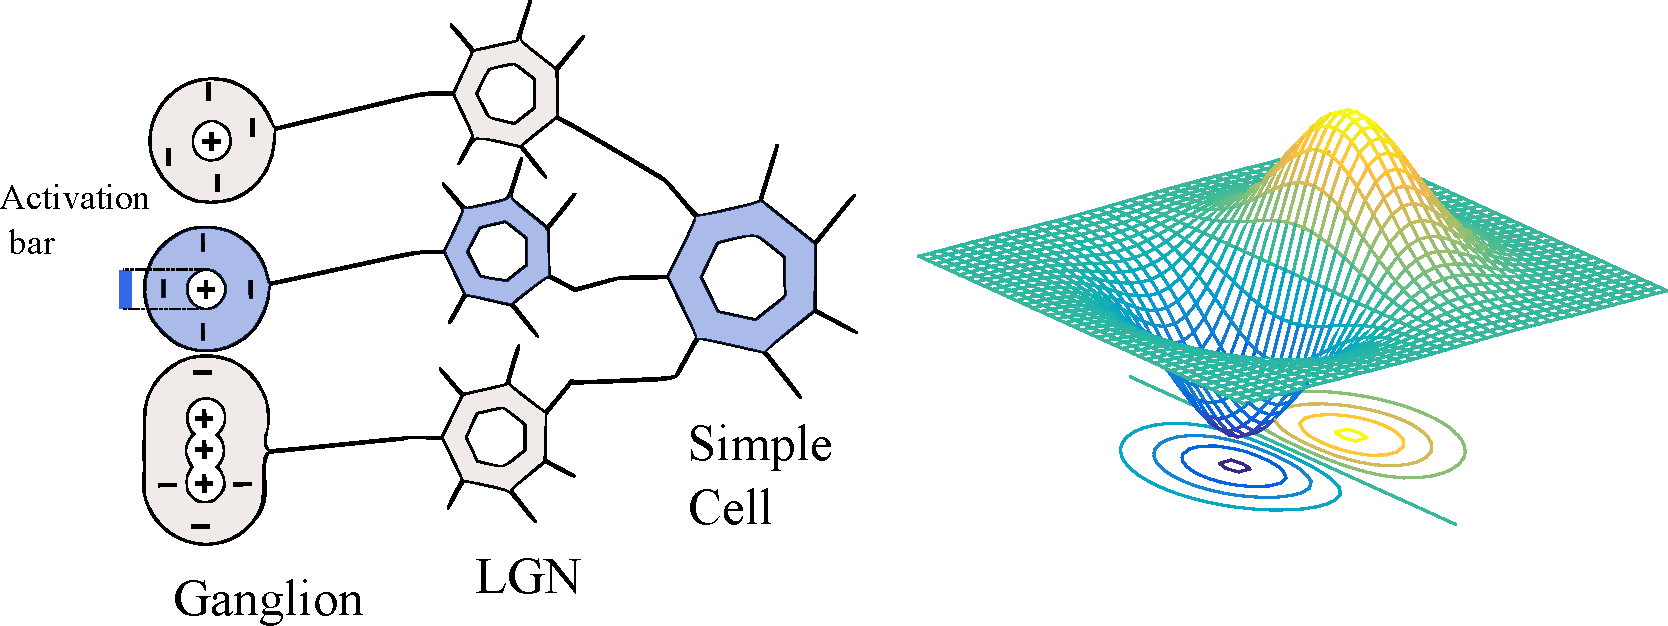
\includegraphics[width=.8\textwidth]{gfx/Chapter05/simple_cell_gabor.pdf}
\caption{Orientation sensitive simple cells which only respond to a bar of certain size and orientation.}
\label{fig:simple_cell}
\end{figure}

Also relevant to this study, the difference of Gaussians (DoG) space representation found in the scale invariant feature transform (SIFT) keypoint detection \cite{lowe2004distinctive} may be seen as an approximation of the spatial receptive field of a retinal ganglion cell. Lowe also suggested that the process behind the computation of the orientation of the frequencies is similar to the behavior of complex cells in V1. In particular, each bin of the histogram of oriented gradients (HOG) can be seen as a single orientation-selective neuron.

We have seen that we can use 2D Gabor like features as a biologically plausible input to place cells models to provide localization. Though differently inspired, we also used SIFT in order to constitute a baseline for our experiments.


\subsection{Biologically Inspired Visual Localization}

Biologically-inspired methods of localisation from image data are emerging; for example, a few computational models for place cell behaviour already exist, though they are often rooted in dynamical systems \cite{blair2008conversion},\cite{bechtel2013investigating}. Some models of place cells use attractor properties of recurrent networks \cite{stringer2002self}, \cite{moser2008place}.  Whilst interesting and valuable, the role of sensory input is marginalized in these models, a key differentiator of the approach we propose here.

The boundary vector cell (BVC) model \cite{barry2006boundary} is a popular computational model that describes place cell response, allowing predictions to be made and experimentally tested \cite{burgess2000predictions}. Whilst of substantial interest in computational neuroscience, one criticism of the BVC model is -- like the dynamical systems models -- a lack of detail in explaining how sensory processing feeds into the computation. The closest work to the approach described in this thesis is Strosslin's \cite{strosslin2005robust}, which uses a low-cost and computationally efficient model to navigate a robot.  However, place cell behaviour -- in terms of firing rates that vary with the position to some reference location -- is not demonstrated except through the policy of a robot and its navigation attempts.  The visual processing is also rather limited, using techniques that are also employed in SLAM algorithms \cite{alcantarilla2010visual} to track specific scene locations. 


Milford and colleagues have also applied SLAM techniques to biologically inspired localisation systems,  setting a seminal precedent with RatSLAM \cite{milford2004ratslam}, a persistent navigation and mapping model based on modelling the hippocampus of rodents. RatSLAM continuously performs SLAM while simultaneously interacting with other navigation systems, such as odometry and landmark detection. More recent work \cite{milford2012seqslam} has been focused on taking RatSLAM to larger scales and incorporating more complex visual landmark detection models. 
%However, we believe those vision models do not capture all the information bandwidth that is required in the same proportion by our brains to provide localization.



\section{Artificial Place Cells (APC)}

\subsection{Modelling a Single Place Cell: the Tuning Curve Encoder}

Given a series of video frames extracted from footage recorded during indoor navigation, we made use of the visual path concept \cite{RiveraWearable, matsumoto1996visual, ohno1996autonomous}, to perform  matching, or association, between locations of a physical environment being traversed and a database of previously captured journeys.

Our proposal -- an evolution of that suggested for sensor and WiFi-based localisation -- is that an appearance-based method using visual features could be easily mined to create a form of \textit{virtual landmarks}.  Such landmarks could be used to retrieve similar image locations around the locale of a landmark. The similarity scores obtained from appearance-based comparison methods, applied between sequences of frames of a journey and these virtual landmarks, should exhibit a behaviour that is similar to those recorded in mammalian place cells (Fig. \ref{fig:BPCdragoi}). In other words, one should obtain high scores when locations are visually similar or spatially close, and low ones when they are dissimilar, with a concave behaviour of scores with distance to the landmark. Requiring such behaviour of location sensing computational units would make them close to the behaviour of biological place cells. 

In order to model the place cell behaviour based on the visual input provided by cameras, we first need a way of describing the collection of patches in an image near to a virtual landmark, and a means of comparing two images through their individual patch similarities. 

We used a subset of the visual features described in detail in Chapter \ref{ch:chapter4}, namely: keypoint-SIFT (SIFT) \cite{lowe2004distinctive}, dense-SIFT (DSIFT)~\cite{vedaldi2010vlfeat}, single-frame (SF-GABOR) and spatio-temporal (ST-GABOR) Gabor based descriptors, and spatio-temporal Gaussian based descriptors~\cite{RiveraWearable}. Table \ref{table:methods} provides a summary of the techniques and shows the number of elements of each descriptor. Similar to the comparison established in the previous chapter, we chose a state-of-the-art SLAM method, Engel's LSD-SLAM~\cite{engel2014lsd}.


\begin{figure}[]
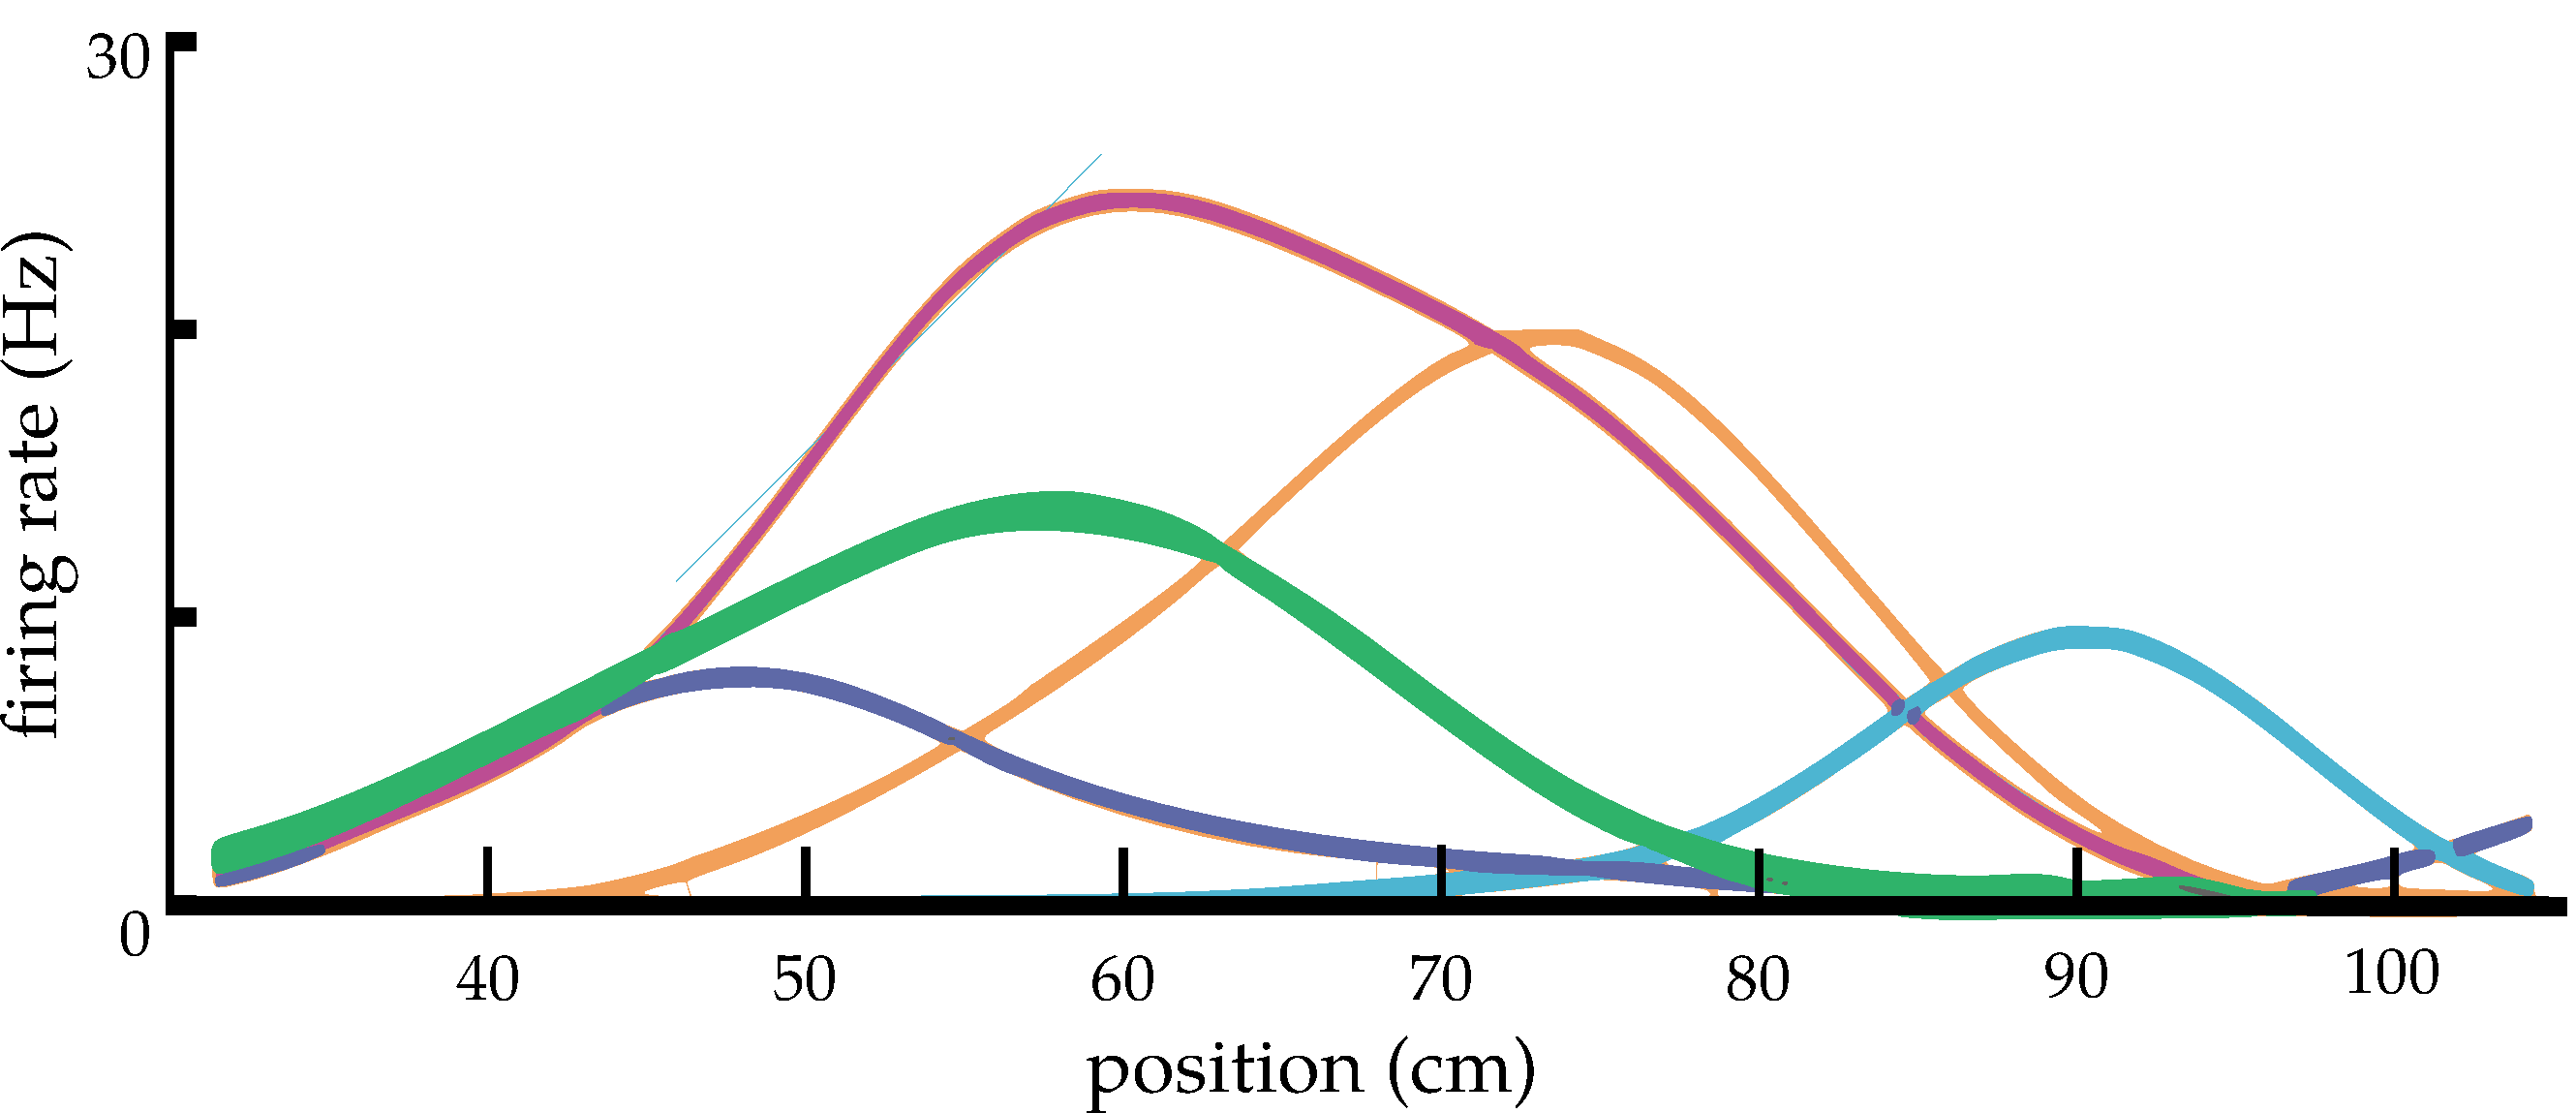
\includegraphics[width=\linewidth]{gfx/Chapter05/dragoi_et_al_place_cell.pdf}
\caption{Firing rates of five BPC recordings covering different place fields of moving rats. Different colors represent different place cells. Adapted from \citep{dragoi2014selection}.}
\label{fig:BPCdragoi}
\end{figure}

\begin{table}
\centering
   \begin{tabular}{lccccc}
    Method          & SIFT & DSIFT & SF-GABOR & ST-GABOR & ST-GAUSS \\ \hline
    ST			   & No   & No    & No       & Yes      & Yes      \\ \hline
    Dense           & No   & Yes   & Yes      & Yes      & Yes      \\ \hline
    Dim.       & 128  & 128   & 136      & 221      & 136      \\
    \end{tabular}
\label{table:methods}
\caption{Summary of the main properties of the different descriptors used. \textbf{ST}: Spatio-temporal, \textbf{SF}: Single-Frame.}
\end{table}



In order to model place cells based on the visual input provided by a camera, we need a way of describing the collection of patches, and comparing two images through their individual patch similarities. When there are several frames involved, the encoding can be computationally expensive, and clumsy to search and compare one frame vs many.  This is the topic we now address.


\subsection{Encoding Frames of Video}

Given a sequence of video frames, each of which is described by a collection of descriptor vectors, the task of comparing frames can be done by comparing vector pairs.  Whilst a pair of frames captured in two different journeys might differ for a number of reasons that include partial occlusion, motion blur, lighting changes and object/scene changes, one would expect that there might be some patches that are similar.  However, in a 1 minute video, one might capture 1,500 frames, with each frame containing several thousand patch descriptors, each of them a high-dimensional vector.

One solution to this ``curse of dimensionality'' is to use the simple vector quantisation approach introduced in Chapter \ref{ch:chapter4} (VQ, $4^{th}$ module of the pipeline described in Fig. \ref{fig:pipeline}, and described as hard assignment, or HA in the previous context), creating a mapping (codebook) that reduces each of the descriptors to a single number representing the identifier of an area of descriptor space.  For this set of experiments, we applied the $k$-means algorithm with $k = 400$ to samples of video data acquired from corridors in order to generate the VQ codebook. Patch descriptors were $L_2$ normalized prior to applying the $k$-means algorithm, then each frame was separately encoded into a 400-element Frame-Encoding Vector (FEV). 


Given a sequence of video frames which are encoded as a set of descriptor vectors the problem of comparing frames can be done by comparing individual vector pairs.  Whilst a pair of frames captured in two different journeys might differ for a number of reasons that include partial occlusion, motion blur, lighting changes and object/scene changes, one would expect that there might be some patches that are similar.  Patch-based comparisons attempt to perform exactly this.  However, in a 1 minute video, one might capture 1,500 frames, with each frame containing several thousand descriptors, each of them a high-dimensional vector.

One solution to this ``curse of dimensionality'' is to use vector quantization (VQ, 4th module of our pipeline described in Fig. \ref{fig:pipeline}), creating a mapping that reduces each of the descriptors to a single number that describes common visual patterns more succinctly.  We applied the $k-$means algorithm with $k = 400$ to samples of video data acquired from corridors in order to generate the codebook; descriptors were first $L_2$ normalized prior to applying the $k-$means algorithm. 


\subsection{Comparing Frames}

In order to model place cell behaviour, we need to map pairs of frames onto a scalar value that is analogous -- perhaps after a non-linearity and affine scaling -- to a firing rate. Consider two image frames that are captured at positions $P$ and $Q$, and are spaced a distance, $\ell_{PQ}$, apart (Fig. \ref{fig:creatingAPCs}). As the distance $\ell_{PQ}$ varies, the mapping should yield a smoothly varying result. In addition, biological place cell (BPC) behaviour often displays a concave relationship between firing rate and distance from the location of peak response (often, the location of some landmark) as illustrated in Fig.~\ref{fig:APC} and Fig.~\ref{fig:creatingAPCs}.


\begin{figure}
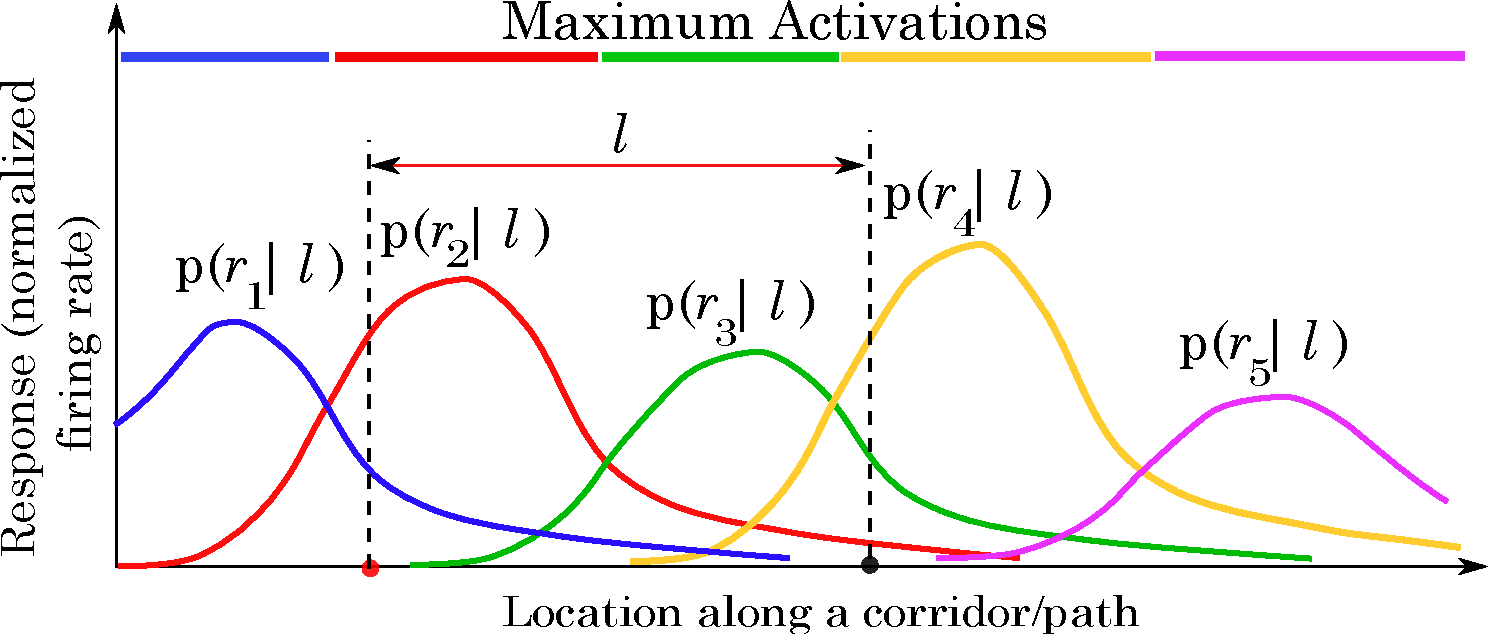
\includegraphics[width=\textwidth]{gfx/Chapter05/APCResponses.pdf}
\label{fig:APC}
\caption{Each curve represents the response -- modelling the firing rate -- of an individual place cell to position along a path. Using the maximum response as an indicator of location allows a simple decoding of place cell responses, localizing a person as being within the ``receptive field'' of a place cell (coloured horizontal bars).}
\end{figure}


\begin{figure}
\includegraphics[width=\textwidth]{gfx/Chapter05/tuning_curves_creation.pdf}
\caption{Illustration of first prototypes of place cell behavior extraction from image descriptor similarities.}
\label{fig:creatingAPCs}
\end{figure}



One way to mimic the behaviour of BPCs within APCs becomes patent when we revisit the \textit{kernel} function we introduced in the previous chapter. This \textit{kernel} maps a pair of FEVs onto a positive scalar value. We used the following mapping between two vectors $\mathbf{v}_a$ and $\mathbf{v}_b$:
\be
\kappa_{\chi^2}(\mathbf{v}_a,\mathbf{v}_b) = \sum_{j=1}^{400}\frac{v_a(j)\cdot v_b(j)}{v_a(j)+v_b(j)}
\ee

This maps the two FEVs onto a scalar value that takes a maximum when the two vectors are identical. The behaviour of this kernel mapping between a fixed frame and a series of frames from a sequence is shown in Fig.~\ref{fig:APCSingleNoisy}.  As one moves along the horizontal axis from left to right, vectors from each frame in a section of a video sequence are compared against those of a {\em reference} frame (virtual visual landmark) from another sequence.  The location of the reference frame corresponds to the location in the new sequence at which one observes the peak in the curve (around frame 690) of Fig.~\ref{fig:APCSingleNoisy}; this location corresponds to the effective position of the virtual landmark, which is the field of view in front of the camera at that (frame) location.  The variability of responses is high, but it is not unlike the types of variation found in biological place cell behaviour.  


%\begin{figure}
%  \centering
%  %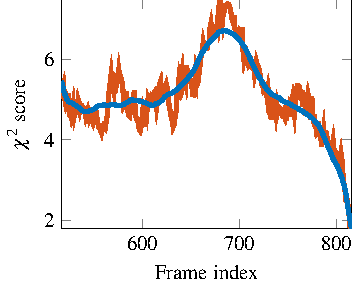
\includegraphics[width=.7\textwidth]{gfx/Chapter05/single_tuning_curve.pdf}
%   \setlength\figureheight{0.3\textwidth}
%	\setlength\figurewidth{0.7\textwidth}
%		% This file was created by matlab2tikz.
% Minimal pgfplots version: 1.3
%
%The latest updates can be retrieved from
%  http://www.mathworks.com/matlabcentral/fileexchange/22022-matlab2tikz
%where you can also make suggestions and rate matlab2tikz.
%
\definecolor{mycolor1}{rgb}{0.00000,0.44700,0.74100}%
\definecolor{mycolor2}{rgb}{0.85000,0.32500,0.09800}%

%
\begin{tikzpicture}

\begin{axis}[%
width=0.95092\figurewidth,
height=\figureheight,
at={(0\figurewidth,0\figureheight)},
scale only axis,
xmin=517,
xmax=816,
xlabel={Frame index},
ymin=1.79650837845272,
ymax=7.47640317281087,
ylabel={$\chi{}^\text{2}\text{ score}$}
]
\addplot [color=mycolor2,solid,line width=2.0pt,forget plot]
  table[row sep=crcr]{%
517	5.45564129617479\\
518	5.28480574819777\\
519	5.38022258546617\\
520	5.04640165964762\\
521	4.91818147235447\\
522	5.02140005429586\\
523	4.9060054090288\\
524	5.14407377772861\\
525	4.78613996505737\\
526	4.74626959694756\\
527	4.60538254843818\\
528	4.73193724950155\\
529	4.89160471492344\\
530	4.61402278476291\\
531	4.74068803257412\\
532	4.82834929890103\\
533	4.78515206442939\\
534	5.00995551215278\\
535	4.93059447076586\\
536	4.747631099489\\
537	4.85051237212287\\
538	4.85323116514418\\
539	4.79317005475362\\
540	4.78844994968838\\
541	4.7296888033549\\
542	4.57528159353468\\
543	4.6541080739763\\
544	4.73621863789029\\
545	4.60128768285116\\
546	4.72721687952677\\
547	4.7022082540724\\
548	4.51559209823608\\
549	4.45021396213108\\
550	4.61597768465678\\
551	4.58577950795492\\
552	4.56056160397\\
553	4.61316866344876\\
554	4.44940259721544\\
555	4.33124679989285\\
556	4.31974034839206\\
557	4.24667429924011\\
558	4.18328481250339\\
559	4.32105019357469\\
560	4.36144169171651\\
561	4.33154243893093\\
562	4.2965227233039\\
563	4.45881326993306\\
564	4.60404780175951\\
565	4.9832649230957\\
566	5.21849367353651\\
567	5.42206896675958\\
568	5.61464606391059\\
569	5.32002242406209\\
570	5.31870725419786\\
571	5.20021793577406\\
572	5.55876763661702\\
573	5.52424425548977\\
574	5.40127817789714\\
575	5.50023322635227\\
576	5.73416566848755\\
577	5.55387417475383\\
578	5.5627646446228\\
579	5.47471041149563\\
580	5.35248724619548\\
581	4.86793337927924\\
582	4.91971654362149\\
583	4.92856052186754\\
584	5.1939090622796\\
585	4.77915970484416\\
586	4.61318797535366\\
587	4.59124125374688\\
588	4.83357630835639\\
589	4.78117969301012\\
590	4.8751319249471\\
591	5.01082160737779\\
592	5.23354652192858\\
593	4.6385703086853\\
594	4.53041002485487\\
595	4.51224210527208\\
596	4.43363348642985\\
597	4.25946267445882\\
598	4.22609305381775\\
599	4.34774973657396\\
600	4.57303765085008\\
601	4.32682673136393\\
602	4.77783237563239\\
603	4.9052480061849\\
604	4.89262798097399\\
605	4.71505321396722\\
606	4.99992277887132\\
607	4.91769223743015\\
608	4.94722530576918\\
609	5.03998618655735\\
610	4.98740741941664\\
611	5.11870463689168\\
612	5.16300662358602\\
613	5.19595686594645\\
614	5.05345845222473\\
615	4.81346085336473\\
616	4.98365359836155\\
617	5.10461118486193\\
618	5.3875585132175\\
619	5.45500458611382\\
620	5.10809373855591\\
621	5.40080017513699\\
622	5.12411006291707\\
623	5.11253976821899\\
624	5.29478883743286\\
625	5.38006231519911\\
626	5.26761012607151\\
627	5.07983054055108\\
628	4.79844037691752\\
629	4.7360757721795\\
630	4.55040812492371\\
631	4.55683490965101\\
632	4.32798796229892\\
633	4.38316342565748\\
634	4.57085434595744\\
635	4.71197700500488\\
636	5.20676475101047\\
637	5.29618379804823\\
638	5.53390868504842\\
639	5.37041934331258\\
640	5.56473557154338\\
641	5.70307895872328\\
642	5.30179659525553\\
643	5.38066954082913\\
644	5.54609791437785\\
645	5.42192618052165\\
646	5.84239138497247\\
647	5.49786647160848\\
648	5.54475773705377\\
649	5.51714981926812\\
650	5.45711406071981\\
651	5.44256104363336\\
652	5.12285571628147\\
653	5.11807007259793\\
654	5.33797539605035\\
655	5.66756502787272\\
656	5.50892194112142\\
657	5.86675696902805\\
658	5.8700491587321\\
659	5.71904346677992\\
660	5.90887721379598\\
661	6.13676097657945\\
662	6.19742769665188\\
663	6.42192517386542\\
664	6.30267741945055\\
665	6.34279457728068\\
666	6.27500221464369\\
667	6.28113868501451\\
668	6.38645627763536\\
669	6.43902895185682\\
670	6.78609715567695\\
671	6.9065891901652\\
672	6.71403990851508\\
673	6.70098299450344\\
674	6.66558986239963\\
675	6.7139032681783\\
676	6.78372716903687\\
677	6.76429753833347\\
678	7.00557661056519\\
679	6.82014653417799\\
680	7.00547329584758\\
681	7.34336815940009\\
682	7.20823060141669\\
683	6.99682813220554\\
684	7.24651824103461\\
685	7.23865800433689\\
686	7.34053574668037\\
687	7.34751473532783\\
688	7.37640317281087\\
689	7.37493318981594\\
690	7.32039319144355\\
691	7.26464568244086\\
692	7.08425818549262\\
693	6.96295788553026\\
694	6.90606005986532\\
695	7.08241897159153\\
696	6.66772707303365\\
697	6.62142117818197\\
698	6.64435042275323\\
699	6.69112764464484\\
700	6.59604427549574\\
701	6.51153024037679\\
702	6.47479195064968\\
703	6.78648434744941\\
704	6.22314156426324\\
705	5.96851372718811\\
706	6.07606569925944\\
707	6.0125810570187\\
708	6.13718112309774\\
709	6.05301419893901\\
710	5.86252167489794\\
711	5.8945533964369\\
712	5.94143915176392\\
713	5.79714462492201\\
714	5.77606577343411\\
715	5.80971254242791\\
716	5.595112880071\\
717	5.6970772213406\\
718	5.93423128128052\\
719	5.84677373038398\\
720	5.82072750727336\\
721	5.70003567801581\\
722	5.5985779232449\\
723	5.41437101364136\\
724	5.41969439718458\\
725	5.26762652397156\\
726	5.31281068589952\\
727	5.33975100517273\\
728	5.22491206063165\\
729	5.03604883617825\\
730	5.22387671470642\\
731	5.00555160310533\\
732	4.94978168275621\\
733	4.51597449514601\\
734	4.7652227083842\\
735	4.92013684908549\\
736	4.85085704591539\\
737	4.84549196561178\\
738	4.6559042930603\\
739	4.86927668253581\\
740	4.71941457854377\\
741	4.81414641274346\\
742	4.79970055156284\\
743	4.69480657577515\\
744	4.71684855884976\\
745	4.59916199578179\\
746	4.60451703601413\\
747	4.55340411927965\\
748	4.76788369814555\\
749	4.70615172386169\\
750	4.6492067972819\\
751	4.7372952832116\\
752	4.70831603474087\\
753	4.95494400130378\\
754	4.93097477489048\\
755	5.05009076330397\\
756	4.83696320321825\\
757	4.65081408288744\\
758	4.9603201813168\\
759	5.27593053711785\\
760	5.34850931167603\\
761	5.34796449873182\\
762	5.31409517923991\\
763	5.15496057934231\\
764	5.20180945926242\\
765	5.18936035368178\\
766	4.8254066573249\\
767	5.08930932150947\\
768	4.86718906296624\\
769	4.62061770757039\\
770	4.98884542783101\\
771	5.15281282530891\\
772	5.03079618348016\\
773	4.79297688272264\\
774	4.88556533389621\\
775	5.0670190387302\\
776	4.6277256541782\\
777	4.46976200739543\\
778	4.50152950816684\\
779	4.35459629694621\\
780	4.15776922967699\\
781	4.18754514058431\\
782	4.16014623641968\\
783	4.23905968666077\\
784	4.11976922882928\\
785	3.84921227561103\\
786	4.09121913380093\\
787	4.26308623949687\\
788	3.93736775716146\\
789	4.12939588228862\\
790	4.14773575464884\\
791	4.02434510654873\\
792	3.93602151340908\\
793	3.89979214138455\\
794	3.81887470351325\\
795	3.75678775045607\\
796	3.81119052569071\\
797	3.97538926866319\\
798	3.73644529448615\\
799	3.62051859166887\\
800	3.63900767432319\\
801	3.4945670498742\\
802	3.44758110576206\\
803	3.41365891032749\\
804	3.53506263097127\\
805	3.68221312099033\\
806	3.50561817487081\\
807	3.18562004301283\\
808	2.92959801355998\\
809	2.77806928422716\\
810	2.53599411911435\\
811	2.5533709526062\\
812	2.44258156087663\\
813	2.23334169387817\\
814	1.9372197786967\\
815	1.97369148996141\\
816	1.79650837845272\\
};


\addplot [color=mycolor1,solid,line width=2.0pt,forget plot]
  table[row sep=crcr]{%
517	5.45564129617479\\
518	5.37355654327958\\
519	5.21705055236816\\
520	5.14466546073792\\
521	5.10476355199461\\
522	5.02677491939429\\
523	4.99369739059709\\
524	4.95151845967328\\
525	4.93448695637821\\
526	4.9382541179657\\
527	4.9249986529981\\
528	4.91614664925469\\
529	4.90358046743605\\
530	4.88218153160786\\
531	4.86746233359151\\
532	4.85760750992751\\
533	4.83489814751879\\
534	4.82152560173519\\
535	4.80884125211217\\
536	4.78737886475022\\
537	4.76278513104612\\
538	4.73903547392951\\
539	4.7215891002137\\
540	4.70695415963518\\
541	4.71049302505528\\
542	4.7056532776545\\
543	4.70845456782923\\
544	4.71323872045054\\
545	4.71882281768349\\
546	4.72699681323131\\
547	4.73064615775128\\
548	4.74396783586532\\
549	4.75172641704412\\
550	4.76428025812248\\
551	4.77966727096748\\
552	4.80270366117257\\
553	4.8194778841369\\
554	4.83317502555933\\
555	4.85074007916613\\
556	4.8632257774033\\
557	4.86403361577836\\
558	4.86677982963942\\
559	4.86511870738871\\
560	4.87049247456246\\
561	4.87113591548807\\
562	4.86629256045197\\
563	4.86094582756631\\
564	4.86177044498677\\
565	4.8616220724015\\
566	4.86459029937277\\
567	4.87347887108385\\
568	4.88530414553186\\
569	4.88331132248686\\
570	4.88186483967061\\
571	4.8774775993797\\
572	4.87199648167271\\
573	4.86676935057521\\
574	4.86219545448719\\
575	4.85672141473039\\
576	4.85646137683029\\
577	4.85169127738935\\
578	4.85505176131147\\
579	4.86435472884146\\
580	4.87581148763903\\
581	4.88387909714056\\
582	4.89925151509222\\
583	4.91423942172338\\
584	4.92701850564572\\
585	4.9408663524792\\
586	4.95425135208095\\
587	4.97103057480723\\
588	4.98540186773893\\
589	4.99748164455907\\
590	4.9989141655617\\
591	4.99064818963983\\
592	4.98170093722354\\
593	4.97129206214092\\
594	4.9726703496747\\
595	4.97545192787707\\
596	4.97357184221955\\
597	4.97034801647506\\
598	4.96218201254501\\
599	4.95628939193933\\
600	4.95209664930832\\
601	4.94487005026162\\
602	4.93902792681912\\
603	4.92917212877684\\
604	4.91537069949974\\
605	4.90279087349941\\
606	4.89631076626767\\
607	4.88890501863562\\
608	4.87664843578728\\
609	4.86010260646846\\
610	4.85585147669526\\
611	4.85786757934121\\
612	4.87042928336699\\
613	4.87987025254438\\
614	4.89523206870842\\
615	4.90533997520568\\
616	4.9166443418213\\
617	4.92622663644977\\
618	4.93976186678793\\
619	4.95711410180782\\
620	4.97821319995283\\
621	4.99838243860777\\
622	5.03068710616927\\
623	5.05664166571602\\
624	5.08107040041969\\
625	5.10033799569353\\
626	5.12340508404773\\
627	5.13697097523142\\
628	5.14141194890686\\
629	5.14601280791959\\
630	5.15872550551313\\
631	5.17235085753356\\
632	5.1844167698538\\
633	5.2031827221652\\
634	5.22012278282183\\
635	5.2350541307272\\
636	5.25118010168443\\
637	5.27105263950062\\
638	5.2914908197191\\
639	5.31941871199748\\
640	5.34981088681556\\
641	5.37754845781391\\
642	5.40143398903395\\
643	5.41967031907062\\
644	5.43867953726494\\
645	5.46584148039353\\
646	5.49411284734332\\
647	5.5304899723892\\
648	5.56317364872178\\
649	5.59187148866199\\
650	5.61810674472731\\
651	5.64762293130092\\
652	5.68239633188226\\
653	5.72251586578871\\
654	5.76883220942923\\
655	5.81515340145483\\
656	5.86512561341802\\
657	5.92666398478744\\
658	5.98431841694579\\
659	6.03382808605289\\
660	6.08555341740044\\
661	6.127020626652\\
662	6.16874209499143\\
663	6.20575446336448\\
664	6.24669290886444\\
665	6.28363571740062\\
666	6.31664213031328\\
667	6.35670027494971\\
668	6.39146739014693\\
669	6.42038289976228\\
670	6.4506713462795\\
671	6.4759780317207\\
672	6.49985273787224\\
673	6.52182546116057\\
674	6.54482955510925\\
675	6.57001350580159\\
676	6.59355397992123\\
677	6.62189427633134\\
678	6.64958247792424\\
679	6.67914388509565\\
680	6.69048218175668\\
681	6.69986160596212\\
682	6.70413321270153\\
683	6.70704202695228\\
684	6.71557544850979\\
685	6.71851701963516\\
686	6.71292029919268\\
687	6.70673919102502\\
688	6.69693335383928\\
689	6.68661635803257\\
690	6.67505046407652\\
691	6.66555475648028\\
692	6.65155422984878\\
693	6.63748526951623\\
694	6.62718327623916\\
695	6.60801341041686\\
696	6.58585296790886\\
697	6.56515900402112\\
698	6.54266094134238\\
699	6.51712586279629\\
700	6.49071343685764\\
701	6.45977260736652\\
702	6.4301504267046\\
703	6.39615398577822\\
704	6.36359818019564\\
705	6.32340584428403\\
706	6.2801509168413\\
707	6.2351982842227\\
708	6.19342182607067\\
709	6.13769644350151\\
710	6.08721817215554\\
711	6.03782227628626\\
712	5.98687007854315\\
713	5.93521882941664\\
714	5.87972844376856\\
715	5.82970565787248\\
716	5.77776216595622\\
717	5.73143335426746\\
718	5.68728524541098\\
719	5.64215762328669\\
720	5.59388067608788\\
721	5.55166506226641\\
722	5.51050375324258\\
723	5.4678313797023\\
724	5.42858150324313\\
725	5.3900122674955\\
726	5.35200566661601\\
727	5.31654655095401\\
728	5.27413495273547\\
729	5.24825336981793\\
730	5.22707910548532\\
731	5.20614084148623\\
732	5.18214864038826\\
733	5.15181461915948\\
734	5.12951474124882\\
735	5.11754349353903\\
736	5.10639973670717\\
737	5.09428800909427\\
738	5.08442985714158\\
739	5.07175424093562\\
740	5.0593480555649\\
741	5.05106739176103\\
742	5.03327819657704\\
743	5.01603489127559\\
744	4.99604336745074\\
745	4.97155133072211\\
746	4.95703724398364\\
747	4.94793999708699\\
748	4.9401119393286\\
749	4.92732178597223\\
750	4.91952461882784\\
751	4.91450846276316\\
752	4.89997733315102\\
753	4.88456610757477\\
754	4.87365754986025\\
755	4.85591713317127\\
756	4.8386154520809\\
757	4.82305960428147\\
758	4.81579780308297\\
759	4.80505978223148\\
760	4.78872574916502\\
761	4.76828401915881\\
762	4.75289069606063\\
763	4.74487400108995\\
764	4.72585545159251\\
765	4.71381425370975\\
766	4.70021403619762\\
767	4.68439045568713\\
768	4.66890504625108\\
769	4.65223042548649\\
770	4.63630619503203\\
771	4.61900559736758\\
772	4.60385838117189\\
773	4.58768502546816\\
774	4.56789509833805\\
775	4.54690146148881\\
776	4.52448742865435\\
777	4.49971704120809\\
778	4.46895453313581\\
779	4.43798890324677\\
780	4.40706996177059\\
781	4.38350363356186\\
782	4.36013228850029\\
783	4.32391391833083\\
784	4.27602958111536\\
785	4.22357162137151\\
786	4.16618447076707\\
787	4.10984316001944\\
788	4.0544884861732\\
789	3.99390751136944\\
790	3.92753729555342\\
791	3.86933902683171\\
792	3.80213900758566\\
793	3.76206392768427\\
794	3.70389658551157\\
795	3.64771100655391\\
796	3.58290216851687\\
797	3.533371826862\\
798	3.48501014709473\\
799	3.44571603063553\\
800	3.400025913611\\
801	3.36231850466848\\
802	3.30612304384224\\
803	3.25225202340648\\
804	3.1855489508311\\
805	3.12186565721668\\
806	3.05844036485783\\
807	2.97056146671897\\
808	2.88727670479444\\
809	2.79667528382054\\
810	2.69914532624758\\
811	2.53378304447791\\
812	2.35337503015259\\
813	2.21038685336946\\
814	2.07666858037313\\
815	1.90247321570361\\
816	1.79650837845272\\
};

\end{axis}
\end{tikzpicture}%

%  \caption{Single APC tuning curve (raw measurements in red) and a smoothed version (blue trace).  The reference frame is located around frame 690. The APC response must be thresholded before using it for accurate position inference; suprathreshold responses from a number of APCs at different positions in the same corridor are shown in Fig.~\ref{fig:APCMany}.}
%  \label{fig:APCSingleNoisy}
%\end{figure}

\begin{figure}[t]
\centering
 \setlength\figureheight{0.6\textwidth}
	\setlength\figurewidth{.9\textwidth}
		% This file was created by matlab2tikz.
% Minimal pgfplots version: 1.3
%
%The latest updates can be retrieved from
%  http://www.mathworks.com/matlabcentral/fileexchange/22022-matlab2tikz
%where you can also make suggestions and rate matlab2tikz.
%
\definecolor{mycolor1}{rgb}{0.00000,0.44700,0.74100}%
\definecolor{mycolor2}{rgb}{0.85000,0.32500,0.09800}%

%
\begin{tikzpicture}

\begin{axis}[%
width=0.95092\figurewidth,
height=\figureheight,
at={(0\figurewidth,0\figureheight)},
scale only axis,
xmin=517,
xmax=816,
xlabel={Frame index},
ymin=1.79650837845272,
ymax=7.47640317281087,
ylabel={$\chi{}^\text{2}\text{ score}$}
]
\addplot [color=mycolor2,solid,line width=2.0pt,forget plot]
  table[row sep=crcr]{%
517	5.45564129617479\\
518	5.28480574819777\\
519	5.38022258546617\\
520	5.04640165964762\\
521	4.91818147235447\\
522	5.02140005429586\\
523	4.9060054090288\\
524	5.14407377772861\\
525	4.78613996505737\\
526	4.74626959694756\\
527	4.60538254843818\\
528	4.73193724950155\\
529	4.89160471492344\\
530	4.61402278476291\\
531	4.74068803257412\\
532	4.82834929890103\\
533	4.78515206442939\\
534	5.00995551215278\\
535	4.93059447076586\\
536	4.747631099489\\
537	4.85051237212287\\
538	4.85323116514418\\
539	4.79317005475362\\
540	4.78844994968838\\
541	4.7296888033549\\
542	4.57528159353468\\
543	4.6541080739763\\
544	4.73621863789029\\
545	4.60128768285116\\
546	4.72721687952677\\
547	4.7022082540724\\
548	4.51559209823608\\
549	4.45021396213108\\
550	4.61597768465678\\
551	4.58577950795492\\
552	4.56056160397\\
553	4.61316866344876\\
554	4.44940259721544\\
555	4.33124679989285\\
556	4.31974034839206\\
557	4.24667429924011\\
558	4.18328481250339\\
559	4.32105019357469\\
560	4.36144169171651\\
561	4.33154243893093\\
562	4.2965227233039\\
563	4.45881326993306\\
564	4.60404780175951\\
565	4.9832649230957\\
566	5.21849367353651\\
567	5.42206896675958\\
568	5.61464606391059\\
569	5.32002242406209\\
570	5.31870725419786\\
571	5.20021793577406\\
572	5.55876763661702\\
573	5.52424425548977\\
574	5.40127817789714\\
575	5.50023322635227\\
576	5.73416566848755\\
577	5.55387417475383\\
578	5.5627646446228\\
579	5.47471041149563\\
580	5.35248724619548\\
581	4.86793337927924\\
582	4.91971654362149\\
583	4.92856052186754\\
584	5.1939090622796\\
585	4.77915970484416\\
586	4.61318797535366\\
587	4.59124125374688\\
588	4.83357630835639\\
589	4.78117969301012\\
590	4.8751319249471\\
591	5.01082160737779\\
592	5.23354652192858\\
593	4.6385703086853\\
594	4.53041002485487\\
595	4.51224210527208\\
596	4.43363348642985\\
597	4.25946267445882\\
598	4.22609305381775\\
599	4.34774973657396\\
600	4.57303765085008\\
601	4.32682673136393\\
602	4.77783237563239\\
603	4.9052480061849\\
604	4.89262798097399\\
605	4.71505321396722\\
606	4.99992277887132\\
607	4.91769223743015\\
608	4.94722530576918\\
609	5.03998618655735\\
610	4.98740741941664\\
611	5.11870463689168\\
612	5.16300662358602\\
613	5.19595686594645\\
614	5.05345845222473\\
615	4.81346085336473\\
616	4.98365359836155\\
617	5.10461118486193\\
618	5.3875585132175\\
619	5.45500458611382\\
620	5.10809373855591\\
621	5.40080017513699\\
622	5.12411006291707\\
623	5.11253976821899\\
624	5.29478883743286\\
625	5.38006231519911\\
626	5.26761012607151\\
627	5.07983054055108\\
628	4.79844037691752\\
629	4.7360757721795\\
630	4.55040812492371\\
631	4.55683490965101\\
632	4.32798796229892\\
633	4.38316342565748\\
634	4.57085434595744\\
635	4.71197700500488\\
636	5.20676475101047\\
637	5.29618379804823\\
638	5.53390868504842\\
639	5.37041934331258\\
640	5.56473557154338\\
641	5.70307895872328\\
642	5.30179659525553\\
643	5.38066954082913\\
644	5.54609791437785\\
645	5.42192618052165\\
646	5.84239138497247\\
647	5.49786647160848\\
648	5.54475773705377\\
649	5.51714981926812\\
650	5.45711406071981\\
651	5.44256104363336\\
652	5.12285571628147\\
653	5.11807007259793\\
654	5.33797539605035\\
655	5.66756502787272\\
656	5.50892194112142\\
657	5.86675696902805\\
658	5.8700491587321\\
659	5.71904346677992\\
660	5.90887721379598\\
661	6.13676097657945\\
662	6.19742769665188\\
663	6.42192517386542\\
664	6.30267741945055\\
665	6.34279457728068\\
666	6.27500221464369\\
667	6.28113868501451\\
668	6.38645627763536\\
669	6.43902895185682\\
670	6.78609715567695\\
671	6.9065891901652\\
672	6.71403990851508\\
673	6.70098299450344\\
674	6.66558986239963\\
675	6.7139032681783\\
676	6.78372716903687\\
677	6.76429753833347\\
678	7.00557661056519\\
679	6.82014653417799\\
680	7.00547329584758\\
681	7.34336815940009\\
682	7.20823060141669\\
683	6.99682813220554\\
684	7.24651824103461\\
685	7.23865800433689\\
686	7.34053574668037\\
687	7.34751473532783\\
688	7.37640317281087\\
689	7.37493318981594\\
690	7.32039319144355\\
691	7.26464568244086\\
692	7.08425818549262\\
693	6.96295788553026\\
694	6.90606005986532\\
695	7.08241897159153\\
696	6.66772707303365\\
697	6.62142117818197\\
698	6.64435042275323\\
699	6.69112764464484\\
700	6.59604427549574\\
701	6.51153024037679\\
702	6.47479195064968\\
703	6.78648434744941\\
704	6.22314156426324\\
705	5.96851372718811\\
706	6.07606569925944\\
707	6.0125810570187\\
708	6.13718112309774\\
709	6.05301419893901\\
710	5.86252167489794\\
711	5.8945533964369\\
712	5.94143915176392\\
713	5.79714462492201\\
714	5.77606577343411\\
715	5.80971254242791\\
716	5.595112880071\\
717	5.6970772213406\\
718	5.93423128128052\\
719	5.84677373038398\\
720	5.82072750727336\\
721	5.70003567801581\\
722	5.5985779232449\\
723	5.41437101364136\\
724	5.41969439718458\\
725	5.26762652397156\\
726	5.31281068589952\\
727	5.33975100517273\\
728	5.22491206063165\\
729	5.03604883617825\\
730	5.22387671470642\\
731	5.00555160310533\\
732	4.94978168275621\\
733	4.51597449514601\\
734	4.7652227083842\\
735	4.92013684908549\\
736	4.85085704591539\\
737	4.84549196561178\\
738	4.6559042930603\\
739	4.86927668253581\\
740	4.71941457854377\\
741	4.81414641274346\\
742	4.79970055156284\\
743	4.69480657577515\\
744	4.71684855884976\\
745	4.59916199578179\\
746	4.60451703601413\\
747	4.55340411927965\\
748	4.76788369814555\\
749	4.70615172386169\\
750	4.6492067972819\\
751	4.7372952832116\\
752	4.70831603474087\\
753	4.95494400130378\\
754	4.93097477489048\\
755	5.05009076330397\\
756	4.83696320321825\\
757	4.65081408288744\\
758	4.9603201813168\\
759	5.27593053711785\\
760	5.34850931167603\\
761	5.34796449873182\\
762	5.31409517923991\\
763	5.15496057934231\\
764	5.20180945926242\\
765	5.18936035368178\\
766	4.8254066573249\\
767	5.08930932150947\\
768	4.86718906296624\\
769	4.62061770757039\\
770	4.98884542783101\\
771	5.15281282530891\\
772	5.03079618348016\\
773	4.79297688272264\\
774	4.88556533389621\\
775	5.0670190387302\\
776	4.6277256541782\\
777	4.46976200739543\\
778	4.50152950816684\\
779	4.35459629694621\\
780	4.15776922967699\\
781	4.18754514058431\\
782	4.16014623641968\\
783	4.23905968666077\\
784	4.11976922882928\\
785	3.84921227561103\\
786	4.09121913380093\\
787	4.26308623949687\\
788	3.93736775716146\\
789	4.12939588228862\\
790	4.14773575464884\\
791	4.02434510654873\\
792	3.93602151340908\\
793	3.89979214138455\\
794	3.81887470351325\\
795	3.75678775045607\\
796	3.81119052569071\\
797	3.97538926866319\\
798	3.73644529448615\\
799	3.62051859166887\\
800	3.63900767432319\\
801	3.4945670498742\\
802	3.44758110576206\\
803	3.41365891032749\\
804	3.53506263097127\\
805	3.68221312099033\\
806	3.50561817487081\\
807	3.18562004301283\\
808	2.92959801355998\\
809	2.77806928422716\\
810	2.53599411911435\\
811	2.5533709526062\\
812	2.44258156087663\\
813	2.23334169387817\\
814	1.9372197786967\\
815	1.97369148996141\\
816	1.79650837845272\\
};


\addplot [color=mycolor1,solid,line width=2.0pt,forget plot]
  table[row sep=crcr]{%
517	5.45564129617479\\
518	5.37355654327958\\
519	5.21705055236816\\
520	5.14466546073792\\
521	5.10476355199461\\
522	5.02677491939429\\
523	4.99369739059709\\
524	4.95151845967328\\
525	4.93448695637821\\
526	4.9382541179657\\
527	4.9249986529981\\
528	4.91614664925469\\
529	4.90358046743605\\
530	4.88218153160786\\
531	4.86746233359151\\
532	4.85760750992751\\
533	4.83489814751879\\
534	4.82152560173519\\
535	4.80884125211217\\
536	4.78737886475022\\
537	4.76278513104612\\
538	4.73903547392951\\
539	4.7215891002137\\
540	4.70695415963518\\
541	4.71049302505528\\
542	4.7056532776545\\
543	4.70845456782923\\
544	4.71323872045054\\
545	4.71882281768349\\
546	4.72699681323131\\
547	4.73064615775128\\
548	4.74396783586532\\
549	4.75172641704412\\
550	4.76428025812248\\
551	4.77966727096748\\
552	4.80270366117257\\
553	4.8194778841369\\
554	4.83317502555933\\
555	4.85074007916613\\
556	4.8632257774033\\
557	4.86403361577836\\
558	4.86677982963942\\
559	4.86511870738871\\
560	4.87049247456246\\
561	4.87113591548807\\
562	4.86629256045197\\
563	4.86094582756631\\
564	4.86177044498677\\
565	4.8616220724015\\
566	4.86459029937277\\
567	4.87347887108385\\
568	4.88530414553186\\
569	4.88331132248686\\
570	4.88186483967061\\
571	4.8774775993797\\
572	4.87199648167271\\
573	4.86676935057521\\
574	4.86219545448719\\
575	4.85672141473039\\
576	4.85646137683029\\
577	4.85169127738935\\
578	4.85505176131147\\
579	4.86435472884146\\
580	4.87581148763903\\
581	4.88387909714056\\
582	4.89925151509222\\
583	4.91423942172338\\
584	4.92701850564572\\
585	4.9408663524792\\
586	4.95425135208095\\
587	4.97103057480723\\
588	4.98540186773893\\
589	4.99748164455907\\
590	4.9989141655617\\
591	4.99064818963983\\
592	4.98170093722354\\
593	4.97129206214092\\
594	4.9726703496747\\
595	4.97545192787707\\
596	4.97357184221955\\
597	4.97034801647506\\
598	4.96218201254501\\
599	4.95628939193933\\
600	4.95209664930832\\
601	4.94487005026162\\
602	4.93902792681912\\
603	4.92917212877684\\
604	4.91537069949974\\
605	4.90279087349941\\
606	4.89631076626767\\
607	4.88890501863562\\
608	4.87664843578728\\
609	4.86010260646846\\
610	4.85585147669526\\
611	4.85786757934121\\
612	4.87042928336699\\
613	4.87987025254438\\
614	4.89523206870842\\
615	4.90533997520568\\
616	4.9166443418213\\
617	4.92622663644977\\
618	4.93976186678793\\
619	4.95711410180782\\
620	4.97821319995283\\
621	4.99838243860777\\
622	5.03068710616927\\
623	5.05664166571602\\
624	5.08107040041969\\
625	5.10033799569353\\
626	5.12340508404773\\
627	5.13697097523142\\
628	5.14141194890686\\
629	5.14601280791959\\
630	5.15872550551313\\
631	5.17235085753356\\
632	5.1844167698538\\
633	5.2031827221652\\
634	5.22012278282183\\
635	5.2350541307272\\
636	5.25118010168443\\
637	5.27105263950062\\
638	5.2914908197191\\
639	5.31941871199748\\
640	5.34981088681556\\
641	5.37754845781391\\
642	5.40143398903395\\
643	5.41967031907062\\
644	5.43867953726494\\
645	5.46584148039353\\
646	5.49411284734332\\
647	5.5304899723892\\
648	5.56317364872178\\
649	5.59187148866199\\
650	5.61810674472731\\
651	5.64762293130092\\
652	5.68239633188226\\
653	5.72251586578871\\
654	5.76883220942923\\
655	5.81515340145483\\
656	5.86512561341802\\
657	5.92666398478744\\
658	5.98431841694579\\
659	6.03382808605289\\
660	6.08555341740044\\
661	6.127020626652\\
662	6.16874209499143\\
663	6.20575446336448\\
664	6.24669290886444\\
665	6.28363571740062\\
666	6.31664213031328\\
667	6.35670027494971\\
668	6.39146739014693\\
669	6.42038289976228\\
670	6.4506713462795\\
671	6.4759780317207\\
672	6.49985273787224\\
673	6.52182546116057\\
674	6.54482955510925\\
675	6.57001350580159\\
676	6.59355397992123\\
677	6.62189427633134\\
678	6.64958247792424\\
679	6.67914388509565\\
680	6.69048218175668\\
681	6.69986160596212\\
682	6.70413321270153\\
683	6.70704202695228\\
684	6.71557544850979\\
685	6.71851701963516\\
686	6.71292029919268\\
687	6.70673919102502\\
688	6.69693335383928\\
689	6.68661635803257\\
690	6.67505046407652\\
691	6.66555475648028\\
692	6.65155422984878\\
693	6.63748526951623\\
694	6.62718327623916\\
695	6.60801341041686\\
696	6.58585296790886\\
697	6.56515900402112\\
698	6.54266094134238\\
699	6.51712586279629\\
700	6.49071343685764\\
701	6.45977260736652\\
702	6.4301504267046\\
703	6.39615398577822\\
704	6.36359818019564\\
705	6.32340584428403\\
706	6.2801509168413\\
707	6.2351982842227\\
708	6.19342182607067\\
709	6.13769644350151\\
710	6.08721817215554\\
711	6.03782227628626\\
712	5.98687007854315\\
713	5.93521882941664\\
714	5.87972844376856\\
715	5.82970565787248\\
716	5.77776216595622\\
717	5.73143335426746\\
718	5.68728524541098\\
719	5.64215762328669\\
720	5.59388067608788\\
721	5.55166506226641\\
722	5.51050375324258\\
723	5.4678313797023\\
724	5.42858150324313\\
725	5.3900122674955\\
726	5.35200566661601\\
727	5.31654655095401\\
728	5.27413495273547\\
729	5.24825336981793\\
730	5.22707910548532\\
731	5.20614084148623\\
732	5.18214864038826\\
733	5.15181461915948\\
734	5.12951474124882\\
735	5.11754349353903\\
736	5.10639973670717\\
737	5.09428800909427\\
738	5.08442985714158\\
739	5.07175424093562\\
740	5.0593480555649\\
741	5.05106739176103\\
742	5.03327819657704\\
743	5.01603489127559\\
744	4.99604336745074\\
745	4.97155133072211\\
746	4.95703724398364\\
747	4.94793999708699\\
748	4.9401119393286\\
749	4.92732178597223\\
750	4.91952461882784\\
751	4.91450846276316\\
752	4.89997733315102\\
753	4.88456610757477\\
754	4.87365754986025\\
755	4.85591713317127\\
756	4.8386154520809\\
757	4.82305960428147\\
758	4.81579780308297\\
759	4.80505978223148\\
760	4.78872574916502\\
761	4.76828401915881\\
762	4.75289069606063\\
763	4.74487400108995\\
764	4.72585545159251\\
765	4.71381425370975\\
766	4.70021403619762\\
767	4.68439045568713\\
768	4.66890504625108\\
769	4.65223042548649\\
770	4.63630619503203\\
771	4.61900559736758\\
772	4.60385838117189\\
773	4.58768502546816\\
774	4.56789509833805\\
775	4.54690146148881\\
776	4.52448742865435\\
777	4.49971704120809\\
778	4.46895453313581\\
779	4.43798890324677\\
780	4.40706996177059\\
781	4.38350363356186\\
782	4.36013228850029\\
783	4.32391391833083\\
784	4.27602958111536\\
785	4.22357162137151\\
786	4.16618447076707\\
787	4.10984316001944\\
788	4.0544884861732\\
789	3.99390751136944\\
790	3.92753729555342\\
791	3.86933902683171\\
792	3.80213900758566\\
793	3.76206392768427\\
794	3.70389658551157\\
795	3.64771100655391\\
796	3.58290216851687\\
797	3.533371826862\\
798	3.48501014709473\\
799	3.44571603063553\\
800	3.400025913611\\
801	3.36231850466848\\
802	3.30612304384224\\
803	3.25225202340648\\
804	3.1855489508311\\
805	3.12186565721668\\
806	3.05844036485783\\
807	2.97056146671897\\
808	2.88727670479444\\
809	2.79667528382054\\
810	2.69914532624758\\
811	2.53378304447791\\
812	2.35337503015259\\
813	2.21038685336946\\
814	2.07666858037313\\
815	1.90247321570361\\
816	1.79650837845272\\
};

\end{axis}
\end{tikzpicture}%

		\label{fig:APCSingleNoisy}
\caption{Single APC tuning curve (raw measurements in red) and a smoothed version (blue trace).  The reference frame is located around frame 690. The APC response must be thresholded before using it for accurate position inference.}
\end{figure}


\begin{figure}
  \centering
  \setlength\figureheight{0.6\textwidth}
  \setlength\figurewidth{.8\textwidth}
  % This file was created by matlab2tikz.
% Minimal pgfplots version: 1.3
%
%The latest updates can be retrieved from
%  http://www.mathworks.com/matlabcentral/fileexchange/22022-matlab2tikz
%where you can also make suggestions and rate matlab2tikz.
%
\definecolor{mycolor1}{rgb}{0.00000,0.44700,0.74100}%
%
\begin{tikzpicture}

\begin{axis}[%
width=\figurewidth,
height=\figureheight,
at={(0\figurewidth,0\figureheight)},
scale only axis,
xmin=0,
xmax=200,
xlabel={Distance covered by place field (cm)},
ymin=6,
ymax=16,
ylabel={$\chi{}^\text{2}\text{ score}$},
axis x line*=bottom,
axis y line*=left,
legend style={at={(0.01,1), font=\footnotesize, pos=north west},anchor=north west,legend cell align=left,align=left,draw=white!15!black}
]
\addplot [color=mycolor1,solid,forget plot]
  table[row sep=crcr]{%
1	7.68376493453979\\
2	8.06428162256877\\
3	8.17457895278931\\
4	8.26771565846034\\
5	8.39854224522909\\
6	8.48510087620128\\
7	8.56682128172654\\
8	8.59774649937948\\
9	8.59330785975737\\
10	8.59233688053332\\
11	8.65034806100946\\
12	8.6829998618678\\
13	8.70982235356381\\
14	8.73964701200786\\
15	8.76372538114849\\
16	8.81391369669061\\
17	8.84981777793482\\
18	8.88881823891087\\
19	8.92264235647101\\
20	8.92992637031957\\
21	8.96761618162456\\
22	8.98679191187808\\
23	8.9777606662951\\
24	8.99128396887528\\
25	9.02349341543097\\
26	9.06194029356304\\
27	9.07705984617534\\
28	9.08789730072021\\
29	9.16552889974494\\
30	9.20696765498111\\
31	9.28507794831928\\
32	9.33594211779143\\
33	9.40688434400056\\
34	9.47275663677015\\
35	9.51096138201262\\
36	9.57157029603657\\
37	9.59795033304315\\
38	9.63532538163035\\
39	9.68495173203318\\
40	9.73211971082185\\
41	9.76160094612523\\
42	9.84171430688155\\
43	9.87884355846204\\
44	9.91074536976061\\
45	9.97806167602539\\
46	10.0605657477128\\
47	10.1543830068488\\
48	10.1903820037842\\
49	10.1771721087004\\
50	10.2039889285439\\
51	10.2577184375964\\
52	10.2896445424933\\
53	10.3242208581222\\
54	10.3520846617849\\
55	10.3246375134117\\
56	10.327644799885\\
57	10.2831729085822\\
58	10.2989949176186\\
59	10.3075340672543\\
60	10.3240774054276\\
61	10.3239422346416\\
62	10.338483057524\\
63	10.355751087791\\
64	10.3346134988885\\
65	10.3087987397846\\
66	10.2878237272564\\
67	10.2445729406256\\
68	10.3025695399234\\
69	10.307963521857\\
70	10.3145902031346\\
71	10.3082494233784\\
72	10.2968946256136\\
73	10.29000347539\\
74	10.3067134556017\\
75	10.3624493950292\\
76	10.4283245990151\\
77	10.473633465014\\
78	10.4986793618453\\
79	10.5597394140143\\
80	10.5885658766094\\
81	10.6724687877454\\
82	10.7098674272236\\
83	10.7820806001362\\
84	10.8456166417975\\
85	10.9124588213469\\
86	10.9945609946\\
87	11.0395386344508\\
88	11.0759984066612\\
89	11.0878075549477\\
90	11.174538913526\\
91	11.2535098226447\\
92	11.2934483477944\\
93	11.4110110433478\\
94	11.4771789249621\\
95	11.5847304494757\\
96	11.6558806770726\\
97	11.6956441778886\\
98	11.741151106985\\
99	11.8461348884984\\
100	11.9315716090955\\
101	12.0584896991127\\
102	12.1596005088405\\
103	12.2862813849198\\
104	12.3939189910889\\
105	12.5373618477269\\
106	12.6995426479139\\
107	12.8576787647448\\
108	13.0239966543097\\
109	13.1540311512194\\
110	13.319268678364\\
111	13.5711681968287\\
112	13.7674868232325\\
113	13.9117409555536\\
114	14.1342613822535\\
115	14.3111799641659\\
116	14.5127577028776\\
117	14.7724789569252\\
118	14.9731010637785\\
119	15.1494964800383\\
120	15.3023914537932\\
121	15.4148659455149\\
122	15.5046606565777\\
123	15.5718047493383\\
124	15.6386499906841\\
125	15.6548606972945\\
126	15.6602967914782\\
127	15.6785095616391\\
128	15.6893093711451\\
129	15.6443962799875\\
130	15.5395172520688\\
131	15.4437499297293\\
132	15.3918147338064\\
133	15.2391425684879\\
134	15.160818150169\\
135	15.0714185112401\\
136	14.8675742902254\\
137	14.6906490827862\\
138	14.4995145295796\\
139	14.317297433552\\
140	14.1889972686768\\
141	14.0079520878039\\
142	13.8699980284038\\
143	13.7053286903783\\
144	13.5121448416459\\
145	13.346944156446\\
146	13.1712456251446\\
147	12.9792186335513\\
148	12.7931142104299\\
149	12.6321003562526\\
150	12.4593344738609\\
151	12.2989568208393\\
152	12.1092826943649\\
153	11.8975028489765\\
154	11.7115875043367\\
155	11.5410103045012\\
156	11.3823467555799\\
157	11.2529855025442\\
158	11.1149904351485\\
159	10.9747475071957\\
160	10.8977248543187\\
161	10.7714399538542\\
162	10.6372470855713\\
163	10.5698853040996\\
164	10.4631252288818\\
165	10.3797384563245\\
166	10.3210554122925\\
167	10.2368787464343\\
168	10.1455332605462\\
169	10.0590010693199\\
170	9.96171790675113\\
171	9.92465465947201\\
172	9.85105524565044\\
173	9.83175578870271\\
174	9.82826910520854\\
175	9.82929244794344\\
176	9.80742454528808\\
177	9.77649437753778\\
178	9.74254201587878\\
179	9.71514656669215\\
180	9.70644775189851\\
181	9.70242635827315\\
182	9.68256599024722\\
183	9.67866546229312\\
184	9.65845037761487\\
185	9.62630086196096\\
186	9.63348855470356\\
187	9.62079033098723\\
188	9.57925399981047\\
189	9.54161443208393\\
190	9.48096516257838\\
191	9.46174189918919\\
192	9.39641958124497\\
193	9.28440195719401\\
194	9.22090192941519\\
195	9.10513149608265\\
196	9.0278107325236\\
197	8.91698932647705\\
198	8.69013175964355\\
199	8.5991382598877\\
200	8.65595436096191\\
};
\addplot [color=mycolor1,solid,forget plot]
  table[row sep=crcr]{%
1	7.78974533081055\\
2	8.24546146392822\\
3	8.2059232711792\\
4	8.30384009225028\\
5	8.46911366780599\\
6	8.57545757293701\\
7	8.66584014892578\\
8	8.72392470041911\\
9	8.77890508315143\\
10	8.76167397750051\\
11	8.81231232693321\\
12	8.84206525902999\\
13	8.89677614914743\\
14	8.95330574637965\\
15	9.03483245247289\\
16	9.11082383206016\\
17	9.16337766145405\\
18	9.21636787213777\\
19	9.25363314779181\\
20	9.32508639285439\\
21	9.37708774365877\\
22	9.41500633641293\\
23	9.44026716131913\\
24	9.4964888723273\\
25	9.51564066033614\\
26	9.57845276280453\\
27	9.61700093118768\\
28	9.67566058510228\\
29	9.76951488695647\\
30	9.84211876517848\\
31	9.88287117606715\\
32	9.90614042784038\\
33	9.95397221414666\\
34	9.94960664447985\\
35	9.94154001537122\\
36	9.93845397547671\\
37	9.93972999171207\\
38	9.94791593049702\\
39	9.91885471343994\\
40	9.86866258320056\\
41	9.8816738630596\\
42	9.86880212081106\\
43	9.85691512258429\\
44	9.86012709768195\\
45	9.86251314062821\\
46	9.85767108515689\\
47	9.86313167371248\\
48	9.88262693505538\\
49	9.85518069016306\\
50	9.86689171038176\\
51	9.85894594694439\\
52	9.86834626448782\\
53	9.87308411849172\\
54	9.89184304287559\\
55	9.88775579552901\\
56	9.86541582408704\\
57	9.83238124847412\\
58	9.82683628483822\\
59	9.85457169382196\\
60	9.84547620070608\\
61	9.87177146108527\\
62	9.89337198357833\\
63	9.93357327109889\\
64	9.95364560578999\\
65	9.97571071825529\\
66	9.97774068932784\\
67	9.96628911871659\\
68	9.99899798945377\\
69	10.0420335468493\\
70	10.0874010889154\\
71	10.1202272114001\\
72	10.1565657163921\\
73	10.1864740974025\\
74	10.2600338082564\\
75	10.3353486312063\\
76	10.4312352130288\\
77	10.5360646498831\\
78	10.6370698025352\\
79	10.700949769271\\
80	10.7748168644152\\
81	10.8565941358867\\
82	10.9276397604691\\
83	10.9812740024767\\
84	11.0603665301674\\
85	11.1463016710783\\
86	11.2400730534604\\
87	11.329712365803\\
88	11.3847010763068\\
89	11.4552882847033\\
90	11.5636912898013\\
91	11.6875077799747\\
92	11.7985651116622\\
93	11.9058998007523\\
94	12.0099947578029\\
95	12.1207789872822\\
96	12.2099598332455\\
97	12.2552975102475\\
98	12.3610138140227\\
99	12.4899568557739\\
100	12.5691422914204\\
101	12.6803599407798\\
102	12.8016963757967\\
103	12.9322004318237\\
104	13.0519447828594\\
105	13.206052077444\\
106	13.3588140387284\\
107	13.5333973734002\\
108	13.7005219710501\\
109	13.8285800532291\\
110	13.9563547937494\\
111	14.0349952798141\\
112	14.1013716647499\\
113	14.1864039772435\\
114	14.2109204342491\\
115	14.2269237919858\\
116	14.266135567113\\
117	14.2827341180099\\
118	14.2736311460796\\
119	14.2758127011751\\
120	14.2420792830618\\
121	14.1923249897204\\
122	14.1247635389629\\
123	14.0710356360988\\
124	14.0194581684313\\
125	13.9296033758866\\
126	13.7861822529843\\
127	13.6250945141441\\
128	13.453824444821\\
129	13.2667096288581\\
130	13.1250362898174\\
131	12.9663466403359\\
132	12.781004554347\\
133	12.6344159276862\\
134	12.5241462807906\\
135	12.4098825454712\\
136	12.2475808294196\\
137	12.0535706469887\\
138	11.9036610251979\\
139	11.7468564384862\\
140	11.6221565447356\\
141	11.4624991667898\\
142	11.3056739004035\\
143	11.1152617805882\\
144	10.9251345082333\\
145	10.801794052124\\
146	10.7027071902626\\
147	10.6084232832256\\
148	10.4968896665071\\
149	10.384888799567\\
150	10.3036232496563\\
151	10.1993318356966\\
152	10.0996779893574\\
153	9.97909385279605\\
154	9.85852597889147\\
155	9.79813359913073\\
156	9.75442550056859\\
157	9.69155070656224\\
158	9.65326334300794\\
159	9.57966924968519\\
160	9.53380233363101\\
161	9.46464528535542\\
162	9.39612448842902\\
163	9.35308556807668\\
164	9.2422446702656\\
165	9.15449970646909\\
166	9.07869484550075\\
167	9.00080003236469\\
168	8.93617208380448\\
169	8.86870073017321\\
170	8.81002882907265\\
171	8.78196811676025\\
172	8.70360577733893\\
173	8.70128056877538\\
174	8.66400911933497\\
175	8.63318400633963\\
176	8.57585036127191\\
177	8.4945794908624\\
178	8.42566879172074\\
179	8.37487855710481\\
180	8.34225682208413\\
181	8.29535717713205\\
182	8.24076075302927\\
183	8.23479767849571\\
184	8.21042311818976\\
185	8.18993523246363\\
186	8.14898566195839\\
187	8.12949215738397\\
188	8.07790214137027\\
189	8.04920269313611\\
190	7.97547782094855\\
191	7.95771581248233\\
192	7.86952066421509\\
193	7.80752712885539\\
194	7.78445606965285\\
195	7.68587064743042\\
196	7.65943537818061\\
197	7.55697100503104\\
198	7.4216682434082\\
199	7.29020881652832\\
200	7.29163646697998\\
};
\addplot [color=mycolor1,solid,forget plot]
  table[row sep=crcr]{%
1	7.53792572021484\\
2	8.41769440968831\\
3	8.45193405151367\\
4	8.43963091714042\\
5	8.55593861473931\\
6	8.53339498693293\\
7	8.54694087688739\\
8	8.57917029062907\\
9	8.58090967290542\\
10	8.57476480383622\\
11	8.62809542605751\\
12	8.60669537594444\\
13	8.6144303271645\\
14	8.62445846356844\\
15	8.65019406770405\\
16	8.7224756542005\\
17	8.74752566688939\\
18	8.77536562869423\\
19	8.8014474166067\\
20	8.82829796640496\\
21	8.87733755613628\\
22	8.91618071104351\\
23	8.92337106403552\\
24	8.92923324986508\\
25	8.9604031412225\\
26	9.0033947794061\\
27	9.0177785471866\\
28	9.05181879746287\\
29	9.13538962916324\\
30	9.19506057940031\\
31	9.31139609688207\\
32	9.3479780899851\\
33	9.44872951507568\\
34	9.52539358640972\\
35	9.56304394571405\\
36	9.64082431793213\\
37	9.68633932816355\\
38	9.76453324368125\\
39	9.84450330232319\\
40	9.91436526649877\\
41	9.97219191099468\\
42	10.07719366174\\
43	10.1646941335578\\
44	10.2257384250039\\
45	10.2896133724012\\
46	10.3917447642276\\
47	10.4897841905293\\
48	10.5431990372507\\
49	10.5694021927683\\
50	10.6057810532419\\
51	10.6896443617971\\
52	10.7062985269647\\
53	10.7471121737832\\
54	10.770522017228\\
55	10.765433261269\\
56	10.768040205303\\
57	10.7172088121113\\
58	10.7385144484671\\
59	10.7417746594078\\
60	10.7527739876195\\
61	10.7460303055613\\
62	10.7402690586291\\
63	10.7531814575195\\
64	10.7657255875437\\
65	10.7440102225856\\
66	10.7015496806095\\
67	10.6753126445569\\
68	10.7077682896664\\
69	10.6848265999242\\
70	10.6560910877429\\
71	10.6374908246492\\
72	10.6371201966938\\
73	10.6588354110718\\
74	10.6684704830772\\
75	10.6907630217703\\
76	10.7655312889501\\
77	10.7710518084074\\
78	10.8048191070557\\
79	10.8590187273527\\
80	10.8969832972476\\
81	10.9915351365742\\
82	11.035874467147\\
83	11.0843456669858\\
84	11.1650513598793\\
85	11.2362122284739\\
86	11.2843780517578\\
87	11.3392468502647\\
88	11.4264742198743\\
89	11.4989445334987\\
90	11.6320958890413\\
91	11.7259882374814\\
92	11.8274932158621\\
93	11.9552382418984\\
94	12.053123072574\\
95	12.1462819952714\\
96	12.2421918166311\\
97	12.3172590356124\\
98	12.3936640086927\\
99	12.4854025087859\\
100	12.534016107258\\
101	12.6280541169016\\
102	12.7412469261571\\
103	12.8599204515156\\
104	12.9735060240093\\
105	13.1089091551931\\
106	13.2714973248933\\
107	13.3795740729884\\
108	13.4991196582192\\
109	13.6079698361849\\
110	13.7665105116995\\
111	13.9488102762323\\
112	14.0583223543669\\
113	14.1919745896992\\
114	14.3112695091649\\
115	14.4063755838495\\
116	14.4961554878636\\
117	14.5627100091231\\
118	14.6310757586831\\
119	14.6866511294716\\
120	14.7194541629992\\
121	14.7554474880821\\
122	14.734463239971\\
123	14.7125848970915\\
124	14.713884654798\\
125	14.6313302391454\\
126	14.5577580803319\\
127	14.4838040502448\\
128	14.3606536764848\\
129	14.1767507352327\\
130	13.9540864542911\\
131	13.7614224584479\\
132	13.5786791851646\\
133	13.3998501426295\\
134	13.2691153978047\\
135	13.1527816872848\\
136	13.0029961937352\\
137	12.8520841598511\\
138	12.6930209210044\\
139	12.5574824684545\\
140	12.4233148976376\\
141	12.2672917717382\\
142	12.1529839666266\\
143	12.0049771258706\\
144	11.8650938335218\\
145	11.7438351982518\\
146	11.6200240787707\\
147	11.4794015382466\\
148	11.3773241545025\\
149	11.278971270511\\
150	11.2159019269441\\
151	11.1297710318314\\
152	11.0236329530415\\
153	10.920069292972\\
154	10.7903712925158\\
155	10.6970327778866\\
156	10.6029547641152\\
157	10.5435114910728\\
158	10.4690053337499\\
159	10.3816188009162\\
160	10.3227086318167\\
161	10.2236641331723\\
162	10.1257185183073\\
163	10.0536445818449\\
164	9.95836252915232\\
165	9.88172621476023\\
166	9.82479893533807\\
167	9.74290541598671\\
168	9.65706197839034\\
169	9.57831091629831\\
170	9.50285986850136\\
171	9.46935648667185\\
172	9.42649675670423\\
173	9.39508282510858\\
174	9.37478396767064\\
175	9.35160902926796\\
176	9.30778377934506\\
177	9.25709302801835\\
178	9.18979996129086\\
179	9.1447222358302\\
180	9.12176332975689\\
181	9.10318354556435\\
182	9.09480471360056\\
183	9.11250797070955\\
184	9.09981747677452\\
185	9.07572073685495\\
186	9.069841033534\\
187	9.06011596478914\\
188	9.01991979699386\\
189	9.00630720038163\\
190	8.92895452599776\\
191	8.85897443169042\\
192	8.80698408800013\\
193	8.73993463516235\\
194	8.69839209776658\\
195	8.64068339087746\\
196	8.54771746529473\\
197	8.3624597958156\\
198	8.20139741897583\\
199	8.11229467391968\\
200	7.99361085891724\\
};
\addplot [color=mycolor1,solid,forget plot]
  table[row sep=crcr]{%
1	7.67510747909546\\
2	8.02797969182332\\
3	8.02783708572388\\
4	8.08701481137957\\
5	8.24081150690714\\
6	8.29345785487782\\
7	8.36440977683434\\
8	8.41121021906535\\
9	8.43581460503971\\
10	8.43798685073853\\
11	8.4774785292776\\
12	8.49419905010023\\
13	8.52700665122584\\
14	8.56879816557232\\
15	8.60205730639006\\
16	8.68092797931872\\
17	8.7052482805754\\
18	8.73601767891332\\
19	8.77790717074745\\
20	8.79095519216437\\
21	8.81890477632221\\
22	8.82694154036672\\
23	8.78551287400095\\
24	8.78290151294909\\
25	8.81253854851973\\
26	8.82332284826981\\
27	8.81395013708817\\
28	8.83184949975264\\
29	8.89935262579667\\
30	8.92547175758763\\
31	9.01900191056101\\
32	9.05566225553814\\
33	9.12206047459652\\
34	9.19217606594688\\
35	9.20620817887156\\
36	9.2657806998805\\
37	9.3228255322105\\
38	9.37231339906391\\
39	9.434991334614\\
40	9.50735473632813\\
41	9.56483499627364\\
42	9.6824019582648\\
43	9.75151307959305\\
44	9.80388099268863\\
45	9.89888898949874\\
46	10.0026696857653\\
47	10.1136653297826\\
48	10.1646432374653\\
49	10.1941034919337\\
50	10.1848286076596\\
51	10.2266358325356\\
52	10.2565713179739\\
53	10.2984978525262\\
54	10.3494261189511\\
55	10.3442784359581\\
56	10.3306920904862\\
57	10.2721648467214\\
58	10.2919540907207\\
59	10.2862624620136\\
60	10.3010430586965\\
61	10.3115950634605\\
62	10.3090416757684\\
63	10.3365298823306\\
64	10.3042678833008\\
65	10.2822478444953\\
66	10.2208267011141\\
67	10.1734511726781\\
68	10.183015923751\\
69	10.1968219656693\\
70	10.1925565819991\\
71	10.1710378747237\\
72	10.1365072350753\\
73	10.1085773267244\\
74	10.1103923697221\\
75	10.1220025012368\\
76	10.1753087796663\\
77	10.1656276301334\\
78	10.1758953395643\\
79	10.1889085267719\\
80	10.2079265996029\\
81	10.260909030312\\
82	10.2833560642443\\
83	10.3270774138601\\
84	10.3511800765991\\
85	10.401598428425\\
86	10.4432211926109\\
87	10.5041371897647\\
88	10.5497394862928\\
89	10.6001655679\\
90	10.663481411181\\
91	10.7435932159424\\
92	10.8124535711188\\
93	10.931635806435\\
94	10.9691206781488\\
95	11.0290167959113\\
96	11.1110087444908\\
97	11.1623848864907\\
98	11.2283980218988\\
99	11.2915564587242\\
100	11.3453365125154\\
101	11.4001959750527\\
102	11.4921314841823\\
103	11.5784212413587\\
104	11.658107707375\\
105	11.7882344597264\\
106	11.8914904845388\\
107	11.9813881422344\\
108	12.1017289914583\\
109	12.2389668916401\\
110	12.354983078806\\
111	12.5136497899106\\
112	12.6622972488403\\
113	12.822884258471\\
114	12.9826191851967\\
115	13.1128613321405\\
116	13.2977402837653\\
117	13.5214897456922\\
118	13.6824388002094\\
119	13.8312137503373\\
120	14.0305517096269\\
121	14.2058560220819\\
122	14.4053375344527\\
123	14.5904177615517\\
124	14.7244217019332\\
125	14.8436335513466\\
126	14.949035744918\\
127	15.0006844369989\\
128	15.0161018371582\\
129	15.0288929186369\\
130	14.9910567936144\\
131	14.9285201022499\\
132	14.9096168216906\\
133	14.8343047091835\\
134	14.7732572555542\\
135	14.6616721404226\\
136	14.5128327419883\\
137	14.4135453073602\\
138	14.2835412778352\\
139	14.0880775953594\\
140	13.9174405148155\\
141	13.6847401669151\\
142	13.4714191838315\\
143	13.2680985802098\\
144	13.0545234680176\\
145	12.8781844691226\\
146	12.7126985851087\\
147	12.5381305594193\\
148	12.3527762262445\\
149	12.1949956793534\\
150	12.0266299498709\\
151	11.8459328099301\\
152	11.6811317644621\\
153	11.5529118086162\\
154	11.4084239758943\\
155	11.2576429969386\\
156	11.0978627455862\\
157	10.9945855391653\\
158	10.8922077480115\\
159	10.7812860890439\\
160	10.7249665511282\\
161	10.6217170012625\\
162	10.5288836328607\\
163	10.469824590181\\
164	10.3625089745773\\
165	10.2785511016846\\
166	10.1991938038876\\
167	10.1336879730225\\
168	10.058065063075\\
169	9.97604274749756\\
170	9.90472442225406\\
171	9.87831226148103\\
172	9.80503383435701\\
173	9.77287568544087\\
174	9.73923577760395\\
175	9.71639005761397\\
176	9.65735601124011\\
177	9.61607802541632\\
178	9.5541854155691\\
179	9.48004250777395\\
180	9.43491443834807\\
181	9.37427671332108\\
182	9.31643320384778\\
183	9.31158899006091\\
184	9.26490452415065\\
185	9.19263538561369\\
186	9.16806421781841\\
187	9.11777009462055\\
188	9.05044116471943\\
189	9.00928720675017\\
190	8.91300756052921\\
191	8.83908319473267\\
192	8.75723325504976\\
193	8.64322557449341\\
194	8.53571477303138\\
195	8.45154064351862\\
196	8.37836027145386\\
197	8.15532091685704\\
198	8.01396207809448\\
199	7.92976951599121\\
200	7.84953498840332\\
};
\addplot [color=mycolor1,solid,forget plot]
  table[row sep=crcr]{%
1	8.81433868408203\\
2	9.23034540812174\\
3	9.2335823059082\\
4	9.34099102020264\\
5	9.54948817359077\\
6	9.62183111364191\\
7	9.69446035531851\\
8	9.789870262146\\
9	9.89363743277157\\
10	9.90569335535953\\
11	9.97196067006964\\
12	9.97963669425563\\
13	10.011661529541\\
14	10.0828073903134\\
15	10.0923711375186\\
16	10.1208186902498\\
17	10.1297840821116\\
18	10.0884271420931\\
19	10.0830247276708\\
20	10.0356542687667\\
21	10.0244679701956\\
22	9.96340726551256\\
23	9.88462889821906\\
24	9.79272837387888\\
25	9.69513120149311\\
26	9.60526702278539\\
27	9.47716226075825\\
28	9.40247194390548\\
29	9.36437140013042\\
30	9.32312734503495\\
31	9.31482922403436\\
32	9.29491384405839\\
33	9.255506264536\\
34	9.23975286985699\\
35	9.20001024948923\\
36	9.19531992862099\\
37	9.19868820591977\\
38	9.18832949588173\\
39	9.17787366164358\\
40	9.18031562002082\\
41	9.23067338843095\\
42	9.26121651498895\\
43	9.31725110505757\\
44	9.3741387818989\\
45	9.44598679793508\\
46	9.51956362473337\\
47	9.59774308455618\\
48	9.66161175778037\\
49	9.68455525448448\\
50	9.70375176479942\\
51	9.7342277326082\\
52	9.75940854925859\\
53	9.80198147422389\\
54	9.83344906254819\\
55	9.84236375909103\\
56	9.84428867540861\\
57	9.84098861092015\\
58	9.90835104490581\\
59	9.94883276286878\\
60	9.96704392684133\\
61	10.0100489666587\\
62	10.0333815122906\\
63	10.0832332309924\\
64	10.1272608606439\\
65	10.1879708641454\\
66	10.2204498993723\\
67	10.2322383177908\\
68	10.2850543574283\\
69	10.3521736044633\\
70	10.4070605227822\\
71	10.4727369609632\\
72	10.5166173734163\\
73	10.571258946469\\
74	10.6429464440597\\
75	10.7131730631778\\
76	10.787567941766\\
77	10.8225504222669\\
78	10.8318123064543\\
79	10.8629351164165\\
80	10.8722321359735\\
81	10.9024934266743\\
82	10.8593071385434\\
83	10.7903524699964\\
84	10.7128779260736\\
85	10.635695658232\\
86	10.5806472176\\
87	10.5005375711541\\
88	10.3787698745728\\
89	10.2658300901714\\
90	10.1498509959171\\
91	10.0393358531751\\
92	9.94387466029117\\
93	9.86416922117534\\
94	9.73504995044909\\
95	9.61683930848774\\
96	9.51589870452881\\
97	9.38871474015085\\
98	9.28313195077996\\
99	9.2079385456286\\
100	9.11097185235274\\
101	9.07585209294369\\
102	9.03614340330425\\
103	9.0284598501105\\
104	8.99892350247032\\
105	8.98294619510048\\
106	8.9573887272885\\
107	8.94512808950324\\
108	8.9349933423494\\
109	8.95447540283203\\
110	8.98234849227102\\
111	8.96920846637926\\
112	8.95385897786994\\
113	8.98447267632735\\
114	9.03605330617804\\
115	9.04860948261462\\
116	9.10419574536775\\
117	9.15457238649067\\
118	9.17053463584498\\
119	9.15528111708792\\
120	9.14118345160233\\
121	9.17276101363333\\
122	9.16511520586516\\
123	9.20452082784552\\
124	9.23201761747661\\
125	9.24844962672183\\
126	9.27211635991146\\
127	9.29224651738217\\
128	9.27942542025917\\
129	9.26802188471744\\
130	9.24410975606818\\
131	9.20184803009033\\
132	9.16427486821225\\
133	9.12231349945068\\
134	9.09987258911133\\
135	9.0798965253328\\
136	9.00989597722104\\
137	8.98267068360981\\
138	8.96830162249113\\
139	8.94864037162379\\
140	8.92396429965371\\
141	8.87839196857653\\
142	8.82449737348055\\
143	8.78394744270726\\
144	8.76934367731998\\
145	8.77443464178788\\
146	8.76824007536236\\
147	8.78366736361855\\
148	8.78206473902652\\
149	8.81885357906944\\
150	8.85141638705605\\
151	8.85671987031636\\
152	8.83402864556563\\
153	8.81142776890805\\
154	8.78990123146459\\
155	8.80176047274941\\
156	8.82996017054508\\
157	8.87393273805317\\
158	8.9145359742014\\
159	8.92137878819516\\
160	8.95175943876568\\
161	8.96687392184609\\
162	8.94563228205631\\
163	8.93641632481625\\
164	8.87744993912546\\
165	8.85818059820878\\
166	8.83726702238384\\
167	8.81949515091745\\
168	8.80027073308041\\
169	8.7787937867014\\
170	8.78570190228914\\
171	8.8056899622867\\
172	8.83311602943822\\
173	8.88890427037289\\
174	8.94124723735609\\
175	8.94182882810894\\
176	8.93705433293393\\
177	8.90617345508776\\
178	8.87179771222566\\
179	8.83730070214522\\
180	8.80530879372045\\
181	8.78288540087248\\
182	8.74752398541099\\
183	8.76241104226363\\
184	8.71782837415996\\
185	8.63711357116699\\
186	8.56437853762978\\
187	8.47666785591527\\
188	8.40000383477462\\
189	8.33727294520328\\
190	8.25480779848601\\
191	8.16453499543039\\
192	8.00565217523014\\
193	7.8574714978536\\
194	7.74527736810538\\
195	7.64499633962458\\
196	7.56967035929362\\
197	7.41352272033691\\
198	7.36305418014526\\
199	7.42254781723022\\
200	7.2355489730835\\
};
\addplot [color=mycolor1,solid,forget plot]
  table[row sep=crcr]{%
1	8.98475742340088\\
2	9.55461184183756\\
3	9.53240470886231\\
4	9.57648658752441\\
5	9.7242743174235\\
6	9.7584753036499\\
7	9.83451850597675\\
8	9.95610637664795\\
9	10.0165695302627\\
10	10.0656920985172\\
11	10.1510985525031\\
12	10.1597460194638\\
13	10.1719956648977\\
14	10.2301388288799\\
15	10.2250874669928\\
16	10.2775150098299\\
17	10.2665961918078\\
18	10.2497899908769\\
19	10.2211738887586\\
20	10.1774712110821\\
21	10.1569156646728\\
22	10.1414686504163\\
23	10.0689720354582\\
24	10.0132412659494\\
25	9.91811968150892\\
26	9.84489179912366\\
27	9.7492497594733\\
28	9.68741687975432\\
29	9.62254569405003\\
30	9.5737439205772\\
31	9.52614553351151\\
32	9.49697358984696\\
33	9.43012659173263\\
34	9.42926582537199\\
35	9.33892591376054\\
36	9.32634182980186\\
37	9.28923591814543\\
38	9.26123639156944\\
39	9.24919374365556\\
40	9.24497298190468\\
41	9.20275120986135\\
42	9.21157365096243\\
43	9.19809597416928\\
44	9.18426257685611\\
45	9.19653280157792\\
46	9.20237445831299\\
47	9.23116538399144\\
48	9.22919057544909\\
49	9.17943076083534\\
50	9.16199282595986\\
51	9.14716800890471\\
52	9.14793150048507\\
53	9.12211091894853\\
54	9.12318043959768\\
55	9.09918554205644\\
56	9.08858936711362\\
57	9.03892276161595\\
58	9.04170026277241\\
59	9.04042143570749\\
60	9.01395928232293\\
61	8.99255536731921\\
62	8.98390875364605\\
63	9.01100575296502\\
64	9.02769560562937\\
65	9.07308387756347\\
66	9.05223434849789\\
67	9.0169015181692\\
68	9.0335774170725\\
69	9.05804719422993\\
70	9.07736441963597\\
71	9.09459324886924\\
72	9.10707990746749\\
73	9.11371592471474\\
74	9.12810541454114\\
75	9.1619045859889\\
76	9.16139191075375\\
77	9.13598401922929\\
78	9.09456248032419\\
79	9.11238258763363\\
80	9.07896578939337\\
81	9.05841556348299\\
82	8.98322572206196\\
83	8.89662815395154\\
84	8.80311667291742\\
85	8.73276431936967\\
86	8.70730999896401\\
87	8.67683277632061\\
88	8.57523401159989\\
89	8.49021713357223\\
90	8.39973005495573\\
91	8.30863513444599\\
92	8.241766151629\\
93	8.16711867483039\\
94	8.05332203915245\\
95	8.02664156963951\\
96	7.97653097855417\\
97	7.89314751876028\\
98	7.79993162657085\\
99	7.77381510483591\\
100	7.74067833549098\\
101	7.69534605427792\\
102	7.69744062423706\\
103	7.67728052641216\\
104	7.66290383589895\\
105	7.628720961119\\
106	7.59444756256907\\
107	7.59042308205052\\
108	7.56735141653764\\
109	7.54788609554893\\
110	7.5318344517758\\
111	7.50550250003212\\
112	7.5006278439572\\
113	7.51268469659906\\
114	7.50924117941605\\
115	7.50656137968365\\
116	7.53768905840422\\
117	7.58197751798128\\
118	7.56859056573165\\
119	7.52485777202406\\
120	7.52684992238095\\
121	7.50847206617656\\
122	7.51437992798655\\
123	7.48842997299997\\
124	7.49423383411608\\
125	7.46874101538407\\
126	7.464574387199\\
127	7.47445437782689\\
128	7.49382131978085\\
129	7.48716959200407\\
130	7.48115732795314\\
131	7.44880179355019\\
132	7.42068140130294\\
133	7.38428055612664\\
134	7.37390590968885\\
135	7.36619788721988\\
136	7.30497239765368\\
137	7.29953665482371\\
138	7.32007997914365\\
139	7.31930135425768\\
140	7.31691701788651\\
141	7.29283009077373\\
142	7.31085195039448\\
143	7.33399830366436\\
144	7.35898534875167\\
145	7.38055409883198\\
146	7.42059669996563\\
147	7.45729157799169\\
148	7.53057833721763\\
149	7.58716299659327\\
150	7.64852840022037\\
151	7.68990980951409\\
152	7.72256567603663\\
153	7.74290940636083\\
154	7.77241573835674\\
155	7.8391843093069\\
156	7.86363812496788\\
157	7.89441673379195\\
158	7.91414873223556\\
159	7.91859671944066\\
160	7.96103281723826\\
161	7.99145658392655\\
162	7.97460977654708\\
163	7.96528605410927\\
164	7.94347338927419\\
165	7.91868270070929\\
166	7.89341414602179\\
167	7.85660088689704\\
168	7.83156093798186\\
169	7.81390759819432\\
170	7.80023592396786\\
171	7.80904910438939\\
172	7.81358001106664\\
173	7.81381574429964\\
174	7.80923913654528\\
175	7.80214693671779\\
176	7.77584168785497\\
177	7.76324081420898\\
178	7.76260644511173\\
179	7.72831291901438\\
180	7.69645690917969\\
181	7.66744335074174\\
182	7.6419388620477\\
183	7.64288693980167\\
184	7.61853072517797\\
185	7.55219690423263\\
186	7.49924750077097\\
187	7.43407906984028\\
188	7.35321777745297\\
189	7.31555765553524\\
190	7.24448828948171\\
191	7.18311450355931\\
192	7.09887176401475\\
193	7.03073581059774\\
194	6.95335953052227\\
195	6.86017916419289\\
196	6.79278013441298\\
197	6.6300208909171\\
198	6.56814556121826\\
199	6.67524846394857\\
200	6.63803768157959\\
};
\addplot [color=mycolor1,solid,forget plot]
  table[row sep=crcr]{%
1	7.42668342590332\\
2	7.7494470278422\\
3	7.72162313461304\\
4	7.753860609872\\
5	7.98453108469645\\
6	8.05623340606689\\
7	8.18162536621094\\
8	8.28020699818929\\
9	8.37644554586971\\
10	8.41024860582854\\
11	8.47356224060059\\
12	8.5127753458525\\
13	8.56745034769962\\
14	8.6504588880037\\
15	8.70380133076718\\
16	8.80214314711721\\
17	8.86353502775493\\
18	8.89925213863975\\
19	8.91904002741764\\
20	8.96249655673378\\
21	9.03348752071983\\
22	9.06271553039551\\
23	9.03724544926694\\
24	9.05558244805587\\
25	9.04643294685765\\
26	9.09303645083779\\
27	9.05124724538703\\
28	9.0558096735101\\
29	9.11467055270546\\
30	9.17829724362022\\
31	9.24240890302156\\
32	9.29634320108514\\
33	9.36129298963045\\
34	9.44331972222579\\
35	9.47070814433851\\
36	9.53372217479505\\
37	9.58285030565764\\
38	9.6662046030948\\
39	9.71602053391306\\
40	9.76563895376105\\
41	9.82438845383493\\
42	9.90105463329114\\
43	9.93708500109221\\
44	9.98212016256232\\
45	10.027766729656\\
46	10.1259446395071\\
47	10.1925515124672\\
48	10.2528242813913\\
49	10.236942190873\\
50	10.2066971628289\\
51	10.2102881983707\\
52	10.1900674920333\\
53	10.1533951006438\\
54	10.1282542881213\\
55	10.0842015115838\\
56	10.0149131072195\\
57	9.8964436681647\\
58	9.83635239852102\\
59	9.79454959066291\\
60	9.72467547968814\\
61	9.6555575822529\\
62	9.60322114040977\\
63	9.57666994396009\\
64	9.5256986618042\\
65	9.45905755695544\\
66	9.40643109773335\\
67	9.30171785856548\\
68	9.26041101154528\\
69	9.24162844607704\\
70	9.18637697320235\\
71	9.15595626831055\\
72	9.1101050627859\\
73	9.06669451061048\\
74	9.03530778382954\\
75	9.0308646151894\\
76	9.02083572588469\\
77	8.9795927248503\\
78	8.90252625314813\\
79	8.8671612488596\\
80	8.83303055010344\\
81	8.81542712763736\\
82	8.78166118421052\\
83	8.71397364766974\\
84	8.64083410564222\\
85	8.57888793945312\\
86	8.56863358146266\\
87	8.53472197683234\\
88	8.46789671245374\\
89	8.40605557592291\\
90	8.32694992266203\\
91	8.28915370138068\\
92	8.26631450653076\\
93	8.25808836284437\\
94	8.21209551158704\\
95	8.20435237884521\\
96	8.18543649974622\\
97	8.1542013820849\\
98	8.12339792753521\\
99	8.10704733196058\\
100	8.06998538970947\\
101	8.02950510225798\\
102	8.01696895298205\\
103	8.01264323686299\\
104	7.98800302806654\\
105	7.95170678590473\\
106	7.92900544718692\\
107	7.93002698295995\\
108	7.93557801999544\\
109	7.94165902388723\\
110	7.95738074654027\\
111	7.92006178906089\\
112	7.87390292318244\\
113	7.87388447711342\\
114	7.84422307265432\\
115	7.82253338161268\\
116	7.83188019300762\\
117	7.84474581166318\\
118	7.81546153520283\\
119	7.7917978136163\\
120	7.79383423453883\\
121	7.795157281976\\
122	7.78530203668695\\
123	7.79192874306127\\
124	7.80357247904727\\
125	7.82046062067935\\
126	7.83675705759149\\
127	7.82696656176918\\
128	7.81252710442794\\
129	7.74503291280646\\
130	7.71488651476408\\
131	7.6857805754009\\
132	7.64233880293997\\
133	7.59959813168174\\
134	7.59633423152723\\
135	7.56641362842761\\
136	7.51193438078228\\
137	7.4954510989942\\
138	7.46076282701994\\
139	7.41463959844489\\
140	7.37203660764192\\
141	7.30360329778571\\
142	7.23198486629285\\
143	7.16897705981606\\
144	7.10406760165566\\
145	7.03936089967427\\
146	6.99705490313078\\
147	6.95970342033788\\
148	6.95316297129581\\
149	6.9500863677577\\
150	6.92944521653025\\
151	6.91123508152209\\
152	6.88309636868929\\
153	6.82230349590904\\
154	6.76661774986669\\
155	6.74287123429148\\
156	6.72443051087229\\
157	6.71816484551681\\
158	6.6981180843554\\
159	6.69512309526142\\
160	6.73731081109298\\
161	6.76232553783216\\
162	6.7640279970671\\
163	6.7598513803984\\
164	6.73353975697568\\
165	6.72791744533338\\
166	6.70602489772596\\
167	6.68838465841193\\
168	6.68887512307418\\
169	6.67725547991301\\
170	6.68373506947568\\
171	6.72130953638177\\
172	6.75745720612375\\
173	6.82813636880172\\
174	6.88470328481574\\
175	6.94321732772024\\
176	7.00632065220883\\
177	7.0836908189874\\
178	7.11392874466745\\
179	7.11077747846905\\
180	7.13311152709158\\
181	7.15295844329031\\
182	7.19379583157991\\
183	7.27317177621942\\
184	7.3285063442431\\
185	7.36771535873413\\
186	7.41875176680715\\
187	7.41792764161762\\
188	7.42798228012888\\
189	7.42943625701101\\
190	7.43177381314729\\
191	7.44348852257979\\
192	7.43298151913811\\
193	7.38401193618774\\
194	7.32309499153724\\
195	7.32124510678378\\
196	7.32649321026272\\
197	7.18282324927194\\
198	7.0601861000061\\
199	7.1346960067749\\
200	7.2848687171936\\
};
\addplot [color=mycolor1,solid,forget plot]
  table[row sep=crcr]{%
1	9.74837207794189\\
2	10.4332828521729\\
3	10.3063383102417\\
4	10.3632534572056\\
5	10.7206337187025\\
6	10.8674935427579\\
7	11.002436197721\\
8	11.1391673405965\\
9	11.2294764238245\\
10	11.2450181559513\\
11	11.3249107662\\
12	11.3248480746621\\
13	11.3036110024703\\
14	11.3699723795841\\
15	11.4074273360403\\
16	11.4430733228985\\
17	11.442511207179\\
18	11.3721434442621\\
19	11.2839701301173\\
20	11.2055451744481\\
21	11.1588952917802\\
22	11.0499616924085\\
23	10.924282124168\\
24	10.7810999217786\\
25	10.6365139107955\\
26	10.5111178849873\\
27	10.3509584226106\\
28	10.219116662678\\
29	10.1191843936318\\
30	10.0261065332513\\
31	9.95929497166684\\
32	9.90977011228862\\
33	9.80244586342259\\
34	9.72630495774118\\
35	9.62724730842992\\
36	9.54649076963726\\
37	9.48334066491378\\
38	9.42168958563554\\
39	9.36929582294665\\
40	9.30510796998677\\
41	9.29804179542943\\
42	9.27339905186703\\
43	9.25389902215255\\
44	9.22667277486701\\
45	9.21345951682643\\
46	9.21456186394942\\
47	9.26005544160542\\
48	9.27277083145945\\
49	9.21958356154592\\
50	9.17184739363821\\
51	9.15906961340653\\
52	9.16107569242778\\
53	9.1183174032914\\
54	9.09432165246261\\
55	9.09380420885588\\
56	9.05617227052387\\
57	9.00296738273219\\
58	8.993745151319\\
59	8.99659653713829\\
60	8.95592443566573\\
61	8.92438858433774\\
62	8.88842793514854\\
63	8.90281310834383\\
64	8.92378596255654\\
65	8.94204782184801\\
66	8.9148352773566\\
67	8.8574440604762\\
68	8.88683630290784\\
69	8.91081649378726\\
70	8.90530927557694\\
71	8.91669328589188\\
72	8.93460303858707\\
73	8.94197579434043\\
74	8.9289866999576\\
75	8.98074496419806\\
76	8.9723068538465\\
77	8.94194096013119\\
78	8.89026973122045\\
79	8.88636046961734\\
80	8.8595276631807\\
81	8.85301868539108\\
82	8.7870266563014\\
83	8.67468776200947\\
84	8.59672481135318\\
85	8.5112486136587\\
86	8.46694185859278\\
87	8.39057560970909\\
88	8.2689101570531\\
89	8.15345701418425\\
90	8.03236248618678\\
91	7.91675961645026\\
92	7.84573580089368\\
93	7.75971894515188\\
94	7.62833494889109\\
95	7.58775301983482\\
96	7.52486728367053\\
97	7.45631453865453\\
98	7.36382692738583\\
99	7.31900280400326\\
100	7.25980961950202\\
101	7.22399033998188\\
102	7.21604558041221\\
103	7.17511523397345\\
104	7.14113699762445\\
105	7.09887303804096\\
106	7.07215939070049\\
107	7.06099058452405\\
108	7.06187273326673\\
109	7.05947276165611\\
110	7.05886599892064\\
111	7.00300512815777\\
112	6.98893953624525\\
113	6.98128180754812\\
114	6.96420541562532\\
115	6.94342035996286\\
116	6.94010245172601\\
117	6.95546832837557\\
118	6.93294402172691\\
119	6.91120739987022\\
120	6.90499483911615\\
121	6.87706445392809\\
122	6.88213958238301\\
123	6.87002307490299\\
124	6.88537459624441\\
125	6.88479461167988\\
126	6.88422607120715\\
127	6.87979986793116\\
128	6.88041774850142\\
129	6.87067450975117\\
130	6.87961626052856\\
131	6.87334070707622\\
132	6.87126879943044\\
133	6.86151885986328\\
134	6.86222814258776\\
135	6.85420661223562\\
136	6.81967278530723\\
137	6.81977216820968\\
138	6.84534286197863\\
139	6.81465271899575\\
140	6.81308555603027\\
141	6.7873844598469\\
142	6.78529285129748\\
143	6.77725553512573\\
144	6.7675878625167\\
145	6.83428370325189\\
146	6.892502784729\\
147	6.95078573728863\\
148	7.03610721387361\\
149	7.12533867986579\\
150	7.19372227317409\\
151	7.25405534945036\\
152	7.30971351422762\\
153	7.36775757137098\\
154	7.42134556017424\\
155	7.50646919953196\\
156	7.58478721819426\\
157	7.65881636268214\\
158	7.74489272268195\\
159	7.82822671689485\\
160	7.9133021706029\\
161	8.00355883648521\\
162	8.07402613288478\\
163	8.14453938132838\\
164	8.14966658542031\\
165	8.16316268318578\\
166	8.19763304057874\\
167	8.21929665615684\\
168	8.23960254066869\\
169	8.25546455383301\\
170	8.25227800168489\\
171	8.26227439077277\\
172	8.28062092630487\\
173	8.32559580551951\\
174	8.38711101130435\\
175	8.4059164147628\\
176	8.41628185071443\\
177	8.44375775989733\\
178	8.43751937464664\\
179	8.42208611337762\\
180	8.36617607819407\\
181	8.31657356964914\\
182	8.27795874445062\\
183	8.25182646199276\\
184	8.19941779186851\\
185	8.0927414894104\\
186	7.98303270339966\\
187	7.84708901455528\\
188	7.74142031920584\\
189	7.68016993372064\\
190	7.60292329286274\\
191	7.50719042828208\\
192	7.33914383719949\\
193	7.16787519454956\\
194	6.9814102099492\\
195	6.85082270882346\\
196	6.71568891737196\\
197	6.55203451429095\\
198	6.48149681091309\\
199	6.62973848978678\\
200	6.49274492263794\\
};
\addplot [color=mycolor1,solid]
  table[row sep=crcr]{%
1	9.51663970947266\\
2	10.2026532491048\\
3	10.0246221542358\\
4	10.0238312312535\\
5	10.2260083092584\\
6	10.2826095927845\\
7	10.3935525600727\\
8	10.4828509012858\\
9	10.5578864041497\\
10	10.5447513680709\\
11	10.5972234324405\\
12	10.5564498399433\\
13	10.5152973375822\\
14	10.5229250757318\\
15	10.5655902561389\\
16	10.5754804611206\\
17	10.5574030123259\\
18	10.4963274002075\\
19	10.4122964959396\\
20	10.3055432470221\\
21	10.2689471495779\\
22	10.1927709077534\\
23	10.0717230345073\\
24	9.975712374637\\
25	9.87063227201763\\
26	9.78159914518658\\
27	9.66112704026072\\
28	9.57529861048648\\
29	9.54441682915939\\
30	9.49475418893915\\
31	9.49588926214921\\
32	9.4766183150442\\
33	9.43909108011346\\
34	9.3884418387162\\
35	9.31237787949411\\
36	9.28372930225573\\
37	9.26992767735531\\
38	9.25808936671207\\
39	9.27296533082661\\
40	9.26257258967349\\
41	9.2439435657702\\
42	9.24004765560752\\
43	9.24186154415733\\
44	9.22901851252506\\
45	9.21912228433709\\
46	9.23918729079397\\
47	9.28860860121877\\
48	9.28283957431191\\
49	9.23684938330399\\
50	9.17693293722052\\
51	9.18452890295731\\
52	9.18824838337145\\
53	9.19768418763813\\
54	9.20294335013942\\
55	9.19531536102295\\
56	9.15106913917943\\
57	9.0814555318732\\
58	9.07087421417236\\
59	9.05045956059506\\
60	9.00431351912649\\
61	8.98440968362909\\
62	8.93695906588906\\
63	8.91816671271073\\
64	8.90299807096782\\
65	8.89827452207866\\
66	8.85612457676938\\
67	8.7812644556949\\
68	8.78641946692216\\
69	8.80674206583123\\
70	8.78844948818809\\
71	8.79170156780042\\
72	8.77566864615992\\
73	8.79307802099931\\
74	8.79395264073422\\
75	8.83406448364258\\
76	8.84910533302709\\
77	8.83968011956466\\
78	8.80826337713944\\
79	8.83551236202842\\
80	8.81516918383146\\
81	8.8045738370795\\
82	8.76991643403706\\
83	8.69805009741532\\
84	8.61889736275924\\
85	8.54774708496897\\
86	8.53670910785073\\
87	8.46752889532792\\
88	8.36375595393934\\
89	8.27062945616873\\
90	8.16327915693584\\
91	8.05363311265644\\
92	7.97532907285188\\
93	7.88930378462139\\
94	7.77230092098838\\
95	7.72283644425241\\
96	7.65743752529747\\
97	7.57849650633963\\
98	7.49435018238268\\
99	7.45804018723337\\
100	7.44104581130178\\
101	7.41871439783197\\
102	7.4325344688014\\
103	7.43720119877866\\
104	7.43186511491474\\
105	7.42055155101575\\
106	7.44126483013756\\
107	7.47406703547428\\
108	7.4669095340528\\
109	7.45994216517398\\
110	7.44897518659893\\
111	7.41945028305054\\
112	7.41423428686042\\
113	7.43059605046323\\
114	7.43771916941593\\
115	7.44811494726884\\
116	7.4748555233604\\
117	7.50266218185425\\
118	7.49779410111277\\
119	7.48908251210263\\
120	7.47906080045198\\
121	7.4467827395389\\
122	7.43904936941047\\
123	7.43780226456492\\
124	7.44929667523033\\
125	7.45702294299477\\
126	7.43693140933388\\
127	7.46912547161705\\
128	7.48484197415804\\
129	7.5102108654223\\
130	7.53065980108161\\
131	7.51496545892013\\
132	7.49722187142623\\
133	7.48440953304893\\
134	7.48927706166317\\
135	7.47615139107955\\
136	7.44537953326577\\
137	7.4228885550248\\
138	7.39254125795866\\
139	7.35240499596847\\
140	7.34017091048391\\
141	7.30194503382633\\
142	7.27028098859285\\
143	7.21997798116584\\
144	7.16640432257401\\
145	7.18757225337781\\
146	7.18869440179122\\
147	7.19198550676045\\
148	7.2246645375302\\
149	7.25589240224738\\
150	7.31456447902479\\
151	7.36559935619957\\
152	7.40011699576127\\
153	7.43229913711548\\
154	7.46079158782959\\
155	7.52046851107949\\
156	7.59446344877544\\
157	7.66742844330637\\
158	7.71506156419453\\
159	7.73533088282535\\
160	7.82586644825183\\
161	7.90827136290701\\
162	7.97432384992901\\
163	8.03526534532246\\
164	8.04044635672318\\
165	8.05734448683889\\
166	8.10454067430998\\
167	8.12944884049265\\
168	8.14523686860737\\
169	8.13581845634862\\
170	8.11790205302991\\
171	8.12166158776534\\
172	8.13165007139507\\
173	8.1524422796149\\
174	8.17301694970382\\
175	8.1803176779496\\
176	8.18188817877519\\
177	8.23093537280434\\
178	8.27313104428743\\
179	8.23055129302175\\
180	8.17268820812828\\
181	8.14570080606561\\
182	8.11043618854723\\
183	8.10645645543149\\
184	8.05729958885594\\
185	7.96570055108321\\
186	7.89043418984664\\
187	7.81569992868524\\
188	7.7526320909199\\
189	7.72511994211297\\
190	7.67025618804129\\
191	7.581442080046\\
192	7.49237733728745\\
193	7.37292296091715\\
194	7.22523924020621\\
195	7.16054777665572\\
196	7.05510854721069\\
197	6.92168930598668\\
198	6.88988704681397\\
199	6.90985012054443\\
200	6.72776651382446\\
};
\addlegendentry{Individual Tuning Curves};

\addplot [color=mycolor1,solid,line width=4.0pt]
  table[row sep=crcr]{%
1	8.3530371983846\\
2	8.88063972967642\\
3	8.85320488611857\\
4	8.90629159836542\\
5	9.09659351537257\\
6	9.16378380553891\\
7	9.25006722996378\\
8	9.32891706537317\\
9	9.38477250641467\\
10	9.39312956625955\\
11	9.45411000056574\\
12	9.46215728012442\\
13	9.47978348481028\\
14	9.52694577222679\\
15	9.56056519279703\\
16	9.61635242149844\\
17	9.63619987867032\\
18	9.63583439274838\\
19	9.63057059572454\\
20	9.61788626442179\\
21	9.63151776163202\\
22	9.61724939402084\\
23	9.56819592303003\\
24	9.5353635542574\\
25	9.4976561975758\\
26	9.47811366521824\\
27	9.42394824334752\\
28	9.39859332815248\\
29	9.41499721237093\\
30	9.41840533206337\\
31	9.44854611402366\\
32	9.45781577260871\\
33	9.46890103747273\\
34	9.4852242386132\\
35	9.46344700194241\\
36	9.47802592160409\\
37	9.48565421745791\\
38	9.50173748864068\\
39	9.51873890837731\\
40	9.53123449024401\\
41	9.55334445886444\\
42	9.59526706160161\\
43	9.62223983786957\\
44	9.64407829931605\\
45	9.68132725654289\\
46	9.73492035112883\\
47	9.7990098027458\\
48	9.83112091488308\\
49	9.81702440384536\\
50	9.80919026491935\\
51	9.82980300390232\\
52	9.84084358549955\\
53	9.84848934307433\\
54	9.86066940374542\\
55	9.84855282097532\\
56	9.82742505324514\\
57	9.77396730791058\\
58	9.77859142370391\\
59	9.78011141883002\\
60	9.76547636623271\\
61	9.7578110276607\\
62	9.74745157587598\\
63	9.76343604974579\\
64	9.76285463745831\\
65	9.76346690752353\\
66	9.73755733311525\\
67	9.69435467636376\\
68	9.71607225540786\\
69	9.73345038207651\\
70	9.73502218235306\\
71	9.74096518510963\\
72	9.7412402002435\\
73	9.7478459453025\\
74	9.7638787888644\\
75	9.80347947349325\\
76	9.84351196065981\\
77	9.85179175549781\\
78	9.84932197325411\\
79	9.87477424688507\\
80	9.8808019955953\\
81	9.91282619230929\\
82	9.9042083171376\\
83	9.88316331272237\\
84	9.866073943021\\
85	9.85587941833407\\
86	9.86916389521102\\
87	9.86475909662526\\
88	9.8323866554171\\
89	9.80315502345213\\
90	9.78955334668968\\
91	9.77979071935018\\
92	9.77833115984822\\
93	9.7935759867841\\
94	9.76783564495064\\
95	9.78213677211115\\
96	9.78657911813747\\
97	9.76682892180325\\
98	9.75431839625041\\
99	9.77543274282712\\
100	9.77806194762737\\
101	9.80116752434892\\
102	9.84375648052372\\
103	9.88750261730618\\
104	9.92225666492306\\
105	9.96926178569682\\
106	10.0239567171063\\
107	10.0836304586533\\
108	10.1435635912488\\
109	10.199220375708\\
110	10.2640579931917\\
111	10.3206501899407\\
112	10.3690046288117\\
113	10.4328803876687\\
114	10.4922791837949\\
115	10.536286691476\\
116	10.6068346681651\\
117	10.6865376729017\\
118	10.7272857364855\\
119	10.757266741747\\
120	10.7933777619524\\
121	10.8187480000725\\
122	10.839467899144\\
123	10.8598386586061\\
124	10.8845455242179\\
125	10.882099631237\\
126	10.8719864616617\\
127	10.8589650399504\\
128	10.8301025440818\\
129	10.7775399252685\\
130	10.7177918277986\\
131	10.6471972995334\\
132	10.5841001153689\\
133	10.5066482142398\\
134	10.4609950020996\\
135	10.4042912143016\\
136	10.3025376810665\\
137	10.2255742619609\\
138	10.1518629224677\\
139	10.0621503305714\\
140	9.99089817972908\\
141	9.88740422711735\\
142	9.80255367881373\\
143	9.7086469443918\\
144	9.61369838491518\\
145	9.55410705254092\\
146	9.49708492714062\\
147	9.43873418004889\\
148	9.39407578406975\\
149	9.35869890346862\\
150	9.32701848403752\\
151	9.28350132947777\\
152	9.22924962238959\\
153	9.16958613144724\\
154	9.10888673548113\\
155	9.07828593393515\\
156	9.04831880435609\\
157	9.03282137363278\\
158	9.01291377084297\\
159	8.97955309438426\\
160	8.98538600631625\\
161	8.9682169574046\\
162	8.93562152929473\\
163	8.92086650335301\\
164	8.86342415893287\\
165	8.82442259927939\\
166	8.79584697533769\\
167	8.75861092896489\\
168	8.72248650991428\\
169	8.68258837091992\\
170	8.64657599744741\\
171	8.6415862339979\\
172	8.62251287315324\\
173	8.63443214851513\\
174	8.64462395439371\\
175	8.64487808071382\\
176	8.62953348884806\\
177	8.61911590475785\\
178	8.59679772282204\\
179	8.56042426371435\\
180	8.53101376204463\\
181	8.50453392943444\\
182	8.47846869697348\\
183	8.48603475302981\\
184	8.46168648011503\\
185	8.41111778794673\\
186	8.37513601849651\\
187	8.32440356204384\\
188	8.26697482281958\\
189	8.23266314065944\\
190	8.16696160578588\\
191	8.11080954088802\\
192	8.02213158015332\\
193	7.92090074397899\\
194	7.8297606900207\\
195	7.74677969710995\\
196	7.67478500177831\\
197	7.52131463610937\\
198	7.40999213324653\\
199	7.41149912940131\\
200	7.3521892759535\\
};
\addlegendentry{Mean};


\addplot[area legend,solid,fill=mycolor1,opacity=1.000000e-01,draw=black]
table[row sep=crcr] {%
x	y\\
1	9.74837207794189\\
2	10.4332828521729\\
3	10.3063383102417\\
4	10.3632534572056\\
5	10.7206337187025\\
6	10.8674935427579\\
7	11.002436197721\\
8	11.1391673405965\\
9	11.2294764238245\\
10	11.2450181559513\\
11	11.3249107662\\
12	11.3248480746621\\
13	11.3036110024703\\
14	11.3699723795841\\
15	11.4074273360403\\
16	11.4430733228985\\
17	11.442511207179\\
18	11.3721434442621\\
19	11.2839701301173\\
20	11.2055451744481\\
21	11.1588952917802\\
22	11.0499616924085\\
23	10.924282124168\\
24	10.7810999217786\\
25	10.6365139107955\\
26	10.5111178849873\\
27	10.3509584226106\\
28	10.219116662678\\
29	10.1191843936318\\
30	10.0261065332513\\
31	9.95929497166684\\
32	9.90977011228862\\
33	9.95397221414666\\
34	9.94960664447985\\
35	9.94154001537122\\
36	9.93845397547671\\
37	9.93972999171207\\
38	9.94791593049702\\
39	9.91885471343994\\
40	9.91436526649877\\
41	9.97219191099468\\
42	10.07719366174\\
43	10.1646941335578\\
44	10.2257384250039\\
45	10.2896133724012\\
46	10.3917447642276\\
47	10.4897841905293\\
48	10.5431990372507\\
49	10.5694021927683\\
50	10.6057810532419\\
51	10.6896443617971\\
52	10.7062985269647\\
53	10.7471121737832\\
54	10.770522017228\\
55	10.765433261269\\
56	10.768040205303\\
57	10.7172088121113\\
58	10.7385144484671\\
59	10.7417746594078\\
60	10.7527739876195\\
61	10.7460303055613\\
62	10.7402690586291\\
63	10.7531814575195\\
64	10.7657255875437\\
65	10.7440102225856\\
66	10.7015496806095\\
67	10.6753126445569\\
68	10.7077682896664\\
69	10.6848265999242\\
70	10.6560910877429\\
71	10.6374908246492\\
72	10.6371201966938\\
73	10.6588354110718\\
74	10.6684704830772\\
75	10.7131730631778\\
76	10.787567941766\\
77	10.8225504222669\\
78	10.8318123064543\\
79	10.8629351164165\\
80	10.8969832972476\\
81	10.9915351365742\\
82	11.035874467147\\
83	11.0843456669858\\
84	11.1650513598793\\
85	11.2362122284739\\
86	11.2843780517578\\
87	11.3392468502647\\
88	11.4264742198743\\
89	11.4989445334987\\
90	11.6320958890413\\
91	11.7259882374814\\
92	11.8274932158621\\
93	11.9552382418984\\
94	12.053123072574\\
95	12.1462819952714\\
96	12.2421918166311\\
97	12.3172590356124\\
98	12.3936640086927\\
99	12.4899568557739\\
100	12.5691422914204\\
101	12.6803599407798\\
102	12.8016963757967\\
103	12.9322004318237\\
104	13.0519447828594\\
105	13.206052077444\\
106	13.3588140387284\\
107	13.5333973734002\\
108	13.7005219710501\\
109	13.8285800532291\\
110	13.9563547937494\\
111	14.0349952798141\\
112	14.1013716647499\\
113	14.1919745896992\\
114	14.3112695091649\\
115	14.4063755838495\\
116	14.5127577028776\\
117	14.7724789569252\\
118	14.9731010637785\\
119	15.1494964800383\\
120	15.3023914537932\\
121	15.4148659455149\\
122	15.5046606565777\\
123	15.5718047493383\\
124	15.6386499906841\\
125	15.6548606972945\\
126	15.6602967914782\\
127	15.6785095616391\\
128	15.6893093711451\\
129	15.6443962799875\\
130	15.5395172520688\\
131	15.4437499297293\\
132	15.3918147338064\\
133	15.2391425684879\\
134	15.160818150169\\
135	15.0714185112401\\
136	14.8675742902254\\
137	14.6906490827862\\
138	14.4995145295796\\
139	14.317297433552\\
140	14.1889972686768\\
141	14.0079520878039\\
142	13.8699980284038\\
143	13.7053286903783\\
144	13.5121448416459\\
145	13.346944156446\\
146	13.1712456251446\\
147	12.9792186335513\\
148	12.7931142104299\\
149	12.6321003562526\\
150	12.4593344738609\\
151	12.2989568208393\\
152	12.1092826943649\\
153	11.8975028489765\\
154	11.7115875043367\\
155	11.5410103045012\\
156	11.3823467555799\\
157	11.2529855025442\\
158	11.1149904351485\\
159	10.9747475071957\\
160	10.8977248543187\\
161	10.7714399538542\\
162	10.6372470855713\\
163	10.5698853040996\\
164	10.4631252288818\\
165	10.3797384563245\\
166	10.3210554122925\\
167	10.2368787464343\\
168	10.1455332605462\\
169	10.0590010693199\\
170	9.96171790675113\\
171	9.92465465947201\\
172	9.85105524565044\\
173	9.83175578870271\\
174	9.82826910520854\\
175	9.82929244794344\\
176	9.80742454528808\\
177	9.77649437753778\\
178	9.74254201587878\\
179	9.71514656669215\\
180	9.70644775189851\\
181	9.70242635827315\\
182	9.68256599024722\\
183	9.67866546229312\\
184	9.65845037761487\\
185	9.62630086196096\\
186	9.63348855470356\\
187	9.62079033098723\\
188	9.57925399981047\\
189	9.54161443208393\\
190	9.48096516257838\\
191	9.46174189918919\\
192	9.39641958124497\\
193	9.28440195719401\\
194	9.22090192941519\\
195	9.10513149608265\\
196	9.0278107325236\\
197	8.91698932647705\\
198	8.69013175964355\\
199	8.5991382598877\\
200	8.65595436096191\\
200	6.49274492263794\\
199	6.62973848978678\\
198	6.48149681091309\\
197	6.55203451429095\\
196	6.71568891737196\\
195	6.85082270882346\\
194	6.95335953052227\\
193	7.03073581059774\\
192	7.09887176401475\\
191	7.18311450355931\\
190	7.24448828948171\\
189	7.31555765553524\\
188	7.35321777745297\\
187	7.41792764161762\\
186	7.41875176680715\\
185	7.36771535873413\\
184	7.3285063442431\\
183	7.27317177621942\\
182	7.19379583157991\\
181	7.15295844329031\\
180	7.13311152709158\\
179	7.11077747846905\\
178	7.11392874466745\\
177	7.0836908189874\\
176	7.00632065220883\\
175	6.94321732772024\\
174	6.88470328481574\\
173	6.82813636880172\\
172	6.75745720612375\\
171	6.72130953638177\\
170	6.68373506947568\\
169	6.67725547991301\\
168	6.68887512307418\\
167	6.68838465841193\\
166	6.70602489772596\\
165	6.72791744533338\\
164	6.73353975697568\\
163	6.7598513803984\\
162	6.7640279970671\\
161	6.76232553783216\\
160	6.73731081109298\\
159	6.69512309526142\\
158	6.6981180843554\\
157	6.71816484551681\\
156	6.72443051087229\\
155	6.74287123429148\\
154	6.76661774986669\\
153	6.82230349590904\\
152	6.88309636868929\\
151	6.91123508152209\\
150	6.92944521653025\\
149	6.9500863677577\\
148	6.95316297129581\\
147	6.95078573728863\\
146	6.892502784729\\
145	6.83428370325189\\
144	6.7675878625167\\
143	6.77725553512573\\
142	6.78529285129748\\
141	6.7873844598469\\
140	6.81308555603027\\
139	6.81465271899575\\
138	6.84534286197863\\
137	6.81977216820968\\
136	6.81967278530723\\
135	6.85420661223562\\
134	6.86222814258776\\
133	6.86151885986328\\
132	6.87126879943044\\
131	6.87334070707622\\
130	6.87961626052856\\
129	6.87067450975117\\
128	6.88041774850142\\
127	6.87979986793116\\
126	6.88422607120715\\
125	6.88479461167988\\
124	6.88537459624441\\
123	6.87002307490299\\
122	6.88213958238301\\
121	6.87706445392809\\
120	6.90499483911615\\
119	6.91120739987022\\
118	6.93294402172691\\
117	6.95546832837557\\
116	6.94010245172601\\
115	6.94342035996286\\
114	6.96420541562532\\
113	6.98128180754812\\
112	6.98893953624525\\
111	7.00300512815777\\
110	7.05886599892064\\
109	7.05947276165611\\
108	7.06187273326673\\
107	7.06099058452405\\
106	7.07215939070049\\
105	7.09887303804096\\
104	7.14113699762445\\
103	7.17511523397345\\
102	7.21604558041221\\
101	7.22399033998188\\
100	7.25980961950202\\
99	7.31900280400326\\
98	7.36382692738583\\
97	7.45631453865453\\
96	7.52486728367053\\
95	7.58775301983482\\
94	7.62833494889109\\
93	7.75971894515188\\
92	7.84573580089368\\
91	7.91675961645026\\
90	8.03236248618678\\
89	8.15345701418425\\
88	8.2689101570531\\
87	8.39057560970909\\
86	8.46694185859278\\
85	8.5112486136587\\
84	8.59672481135318\\
83	8.67468776200947\\
82	8.76991643403706\\
81	8.8045738370795\\
80	8.81516918383146\\
79	8.83551236202842\\
78	8.80826337713944\\
77	8.83968011956466\\
76	8.84910533302709\\
75	8.83406448364258\\
74	8.79395264073422\\
73	8.79307802099931\\
72	8.77566864615992\\
71	8.79170156780042\\
70	8.78844948818809\\
69	8.80674206583123\\
68	8.78641946692216\\
67	8.7812644556949\\
66	8.85612457676938\\
65	8.89827452207866\\
64	8.90299807096782\\
63	8.90281310834383\\
62	8.88842793514854\\
61	8.92438858433774\\
60	8.95592443566573\\
59	8.99659653713829\\
58	8.993745151319\\
57	9.00296738273219\\
56	9.05617227052387\\
55	9.09380420885588\\
54	9.09432165246261\\
53	9.1183174032914\\
52	9.14793150048507\\
51	9.14716800890471\\
50	9.16199282595986\\
49	9.17943076083534\\
48	9.22919057544909\\
47	9.23116538399144\\
46	9.20237445831299\\
45	9.19653280157792\\
44	9.18426257685611\\
43	9.19809597416928\\
42	9.21157365096243\\
41	9.20275120986135\\
40	9.18031562002082\\
39	9.17787366164358\\
38	9.18832949588173\\
37	9.19868820591977\\
36	9.19531992862099\\
35	9.20001024948923\\
34	9.19217606594688\\
33	9.12206047459652\\
32	9.05566225553814\\
31	9.01900191056101\\
30	8.92547175758763\\
29	8.89935262579667\\
28	8.83184949975264\\
27	8.81395013708817\\
26	8.82332284826981\\
25	8.81253854851973\\
24	8.78290151294909\\
23	8.78551287400095\\
22	8.82694154036672\\
21	8.81890477632221\\
20	8.79095519216437\\
19	8.77790717074745\\
18	8.73601767891332\\
17	8.7052482805754\\
16	8.68092797931872\\
15	8.60205730639006\\
14	8.56879816557232\\
13	8.52700665122584\\
12	8.49419905010023\\
11	8.47356224060059\\
10	8.41024860582854\\
9	8.37644554586971\\
8	8.28020699818929\\
7	8.18162536621094\\
6	8.05623340606689\\
5	7.98453108469645\\
4	7.753860609872\\
3	7.72162313461304\\
2	7.7494470278422\\
1	7.42668342590332\\
}--cycle;

\addlegendentry{Variability};

\end{axis}
\end{tikzpicture}%
  %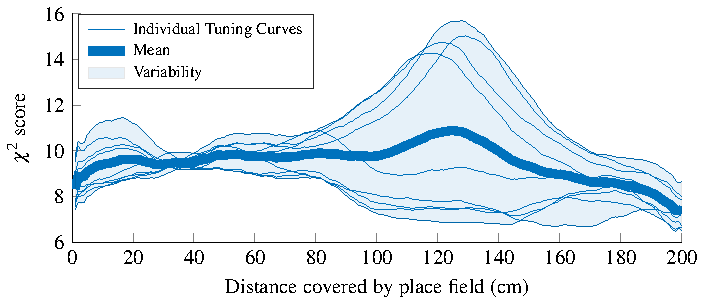
\includegraphics[width=4.5in]{gfx/Chapter05/receptive_place_field.pdf}
  \caption{The variability of individual artificial place field (APC) responses, displayed using mean and standard deviation (envelopes) of response over ensembles. \td{Improve}{To change to mean $\pm$ 1 s.d.}.}
  \label{fig:APCVariability}
\end{figure}



\section{Creating Place Fields}

The similarity function $\kappa_{\chi^2}$ is an important component in producing APC behaviour from FEVs.  However, regions of the APC response curve which are almost flat contain very little information from the point of inferring the position of a stimulus that elicits some response. In other words, regions of the curve where the gradient with respect to distance to the peak of the curve, $\ell$, is small, convey relatively little information about the camera's location. Other regions of the curve show rapid change with distance from the peak. In order to synthesize useful ``tuning curves'' for APCs, we need to define sub- and supra-threshold regions for each APC that we wish to define (Fig.~\ref{fig:Supra}).

\begin{figure}
\centering
  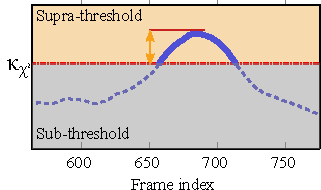
\includegraphics[width=\linewidth]{gfx/Chapter05/tuning_curve-thresh.pdf}
\caption{Sub-threshold and supra-threshold regions can be identified by setting a threshold on the amplitude of the $\kappa_{\chi^2}$ similarity measure; the height of the threshold controls the support region of supra-threshold region of an artificial place cell.}
\label{fig:Supra}
\end{figure}


%\begin{figure}
%  \centering
%  %\setlength\figureheight{0.2\textwidth}
%  %\setlength\figurewidth{0.4\textwidth}
%  %% This file was created by matlab2tikz.
% Minimal pgfplots version: 1.3
%
%The latest updates can be retrieved from
%  http://www.mathworks.com/matlabcentral/fileexchange/22022-matlab2tikz
%where you can also make suggestions and rate matlab2tikz.
%
\definecolor{mycolor1}{rgb}{0.00000,0.44700,0.74100}%
%
\begin{tikzpicture}

\begin{axis}[%
width=\figurewidth,
height=\figureheight,
at={(0\figurewidth,0\figureheight)},
scale only axis,
xmin=0,
xmax=200,
xlabel={Distance covered by place field (cm)},
ymin=6,
ymax=16,
ylabel={$\chi{}^\text{2}\text{ score}$},
axis x line*=bottom,
axis y line*=left,
legend style={at={(0.01,1), font=\footnotesize, pos=north west},anchor=north west,legend cell align=left,align=left,draw=white!15!black}
]
\addplot [color=mycolor1,solid,forget plot]
  table[row sep=crcr]{%
1	7.68376493453979\\
2	8.06428162256877\\
3	8.17457895278931\\
4	8.26771565846034\\
5	8.39854224522909\\
6	8.48510087620128\\
7	8.56682128172654\\
8	8.59774649937948\\
9	8.59330785975737\\
10	8.59233688053332\\
11	8.65034806100946\\
12	8.6829998618678\\
13	8.70982235356381\\
14	8.73964701200786\\
15	8.76372538114849\\
16	8.81391369669061\\
17	8.84981777793482\\
18	8.88881823891087\\
19	8.92264235647101\\
20	8.92992637031957\\
21	8.96761618162456\\
22	8.98679191187808\\
23	8.9777606662951\\
24	8.99128396887528\\
25	9.02349341543097\\
26	9.06194029356304\\
27	9.07705984617534\\
28	9.08789730072021\\
29	9.16552889974494\\
30	9.20696765498111\\
31	9.28507794831928\\
32	9.33594211779143\\
33	9.40688434400056\\
34	9.47275663677015\\
35	9.51096138201262\\
36	9.57157029603657\\
37	9.59795033304315\\
38	9.63532538163035\\
39	9.68495173203318\\
40	9.73211971082185\\
41	9.76160094612523\\
42	9.84171430688155\\
43	9.87884355846204\\
44	9.91074536976061\\
45	9.97806167602539\\
46	10.0605657477128\\
47	10.1543830068488\\
48	10.1903820037842\\
49	10.1771721087004\\
50	10.2039889285439\\
51	10.2577184375964\\
52	10.2896445424933\\
53	10.3242208581222\\
54	10.3520846617849\\
55	10.3246375134117\\
56	10.327644799885\\
57	10.2831729085822\\
58	10.2989949176186\\
59	10.3075340672543\\
60	10.3240774054276\\
61	10.3239422346416\\
62	10.338483057524\\
63	10.355751087791\\
64	10.3346134988885\\
65	10.3087987397846\\
66	10.2878237272564\\
67	10.2445729406256\\
68	10.3025695399234\\
69	10.307963521857\\
70	10.3145902031346\\
71	10.3082494233784\\
72	10.2968946256136\\
73	10.29000347539\\
74	10.3067134556017\\
75	10.3624493950292\\
76	10.4283245990151\\
77	10.473633465014\\
78	10.4986793618453\\
79	10.5597394140143\\
80	10.5885658766094\\
81	10.6724687877454\\
82	10.7098674272236\\
83	10.7820806001362\\
84	10.8456166417975\\
85	10.9124588213469\\
86	10.9945609946\\
87	11.0395386344508\\
88	11.0759984066612\\
89	11.0878075549477\\
90	11.174538913526\\
91	11.2535098226447\\
92	11.2934483477944\\
93	11.4110110433478\\
94	11.4771789249621\\
95	11.5847304494757\\
96	11.6558806770726\\
97	11.6956441778886\\
98	11.741151106985\\
99	11.8461348884984\\
100	11.9315716090955\\
101	12.0584896991127\\
102	12.1596005088405\\
103	12.2862813849198\\
104	12.3939189910889\\
105	12.5373618477269\\
106	12.6995426479139\\
107	12.8576787647448\\
108	13.0239966543097\\
109	13.1540311512194\\
110	13.319268678364\\
111	13.5711681968287\\
112	13.7674868232325\\
113	13.9117409555536\\
114	14.1342613822535\\
115	14.3111799641659\\
116	14.5127577028776\\
117	14.7724789569252\\
118	14.9731010637785\\
119	15.1494964800383\\
120	15.3023914537932\\
121	15.4148659455149\\
122	15.5046606565777\\
123	15.5718047493383\\
124	15.6386499906841\\
125	15.6548606972945\\
126	15.6602967914782\\
127	15.6785095616391\\
128	15.6893093711451\\
129	15.6443962799875\\
130	15.5395172520688\\
131	15.4437499297293\\
132	15.3918147338064\\
133	15.2391425684879\\
134	15.160818150169\\
135	15.0714185112401\\
136	14.8675742902254\\
137	14.6906490827862\\
138	14.4995145295796\\
139	14.317297433552\\
140	14.1889972686768\\
141	14.0079520878039\\
142	13.8699980284038\\
143	13.7053286903783\\
144	13.5121448416459\\
145	13.346944156446\\
146	13.1712456251446\\
147	12.9792186335513\\
148	12.7931142104299\\
149	12.6321003562526\\
150	12.4593344738609\\
151	12.2989568208393\\
152	12.1092826943649\\
153	11.8975028489765\\
154	11.7115875043367\\
155	11.5410103045012\\
156	11.3823467555799\\
157	11.2529855025442\\
158	11.1149904351485\\
159	10.9747475071957\\
160	10.8977248543187\\
161	10.7714399538542\\
162	10.6372470855713\\
163	10.5698853040996\\
164	10.4631252288818\\
165	10.3797384563245\\
166	10.3210554122925\\
167	10.2368787464343\\
168	10.1455332605462\\
169	10.0590010693199\\
170	9.96171790675113\\
171	9.92465465947201\\
172	9.85105524565044\\
173	9.83175578870271\\
174	9.82826910520854\\
175	9.82929244794344\\
176	9.80742454528808\\
177	9.77649437753778\\
178	9.74254201587878\\
179	9.71514656669215\\
180	9.70644775189851\\
181	9.70242635827315\\
182	9.68256599024722\\
183	9.67866546229312\\
184	9.65845037761487\\
185	9.62630086196096\\
186	9.63348855470356\\
187	9.62079033098723\\
188	9.57925399981047\\
189	9.54161443208393\\
190	9.48096516257838\\
191	9.46174189918919\\
192	9.39641958124497\\
193	9.28440195719401\\
194	9.22090192941519\\
195	9.10513149608265\\
196	9.0278107325236\\
197	8.91698932647705\\
198	8.69013175964355\\
199	8.5991382598877\\
200	8.65595436096191\\
};
\addplot [color=mycolor1,solid,forget plot]
  table[row sep=crcr]{%
1	7.78974533081055\\
2	8.24546146392822\\
3	8.2059232711792\\
4	8.30384009225028\\
5	8.46911366780599\\
6	8.57545757293701\\
7	8.66584014892578\\
8	8.72392470041911\\
9	8.77890508315143\\
10	8.76167397750051\\
11	8.81231232693321\\
12	8.84206525902999\\
13	8.89677614914743\\
14	8.95330574637965\\
15	9.03483245247289\\
16	9.11082383206016\\
17	9.16337766145405\\
18	9.21636787213777\\
19	9.25363314779181\\
20	9.32508639285439\\
21	9.37708774365877\\
22	9.41500633641293\\
23	9.44026716131913\\
24	9.4964888723273\\
25	9.51564066033614\\
26	9.57845276280453\\
27	9.61700093118768\\
28	9.67566058510228\\
29	9.76951488695647\\
30	9.84211876517848\\
31	9.88287117606715\\
32	9.90614042784038\\
33	9.95397221414666\\
34	9.94960664447985\\
35	9.94154001537122\\
36	9.93845397547671\\
37	9.93972999171207\\
38	9.94791593049702\\
39	9.91885471343994\\
40	9.86866258320056\\
41	9.8816738630596\\
42	9.86880212081106\\
43	9.85691512258429\\
44	9.86012709768195\\
45	9.86251314062821\\
46	9.85767108515689\\
47	9.86313167371248\\
48	9.88262693505538\\
49	9.85518069016306\\
50	9.86689171038176\\
51	9.85894594694439\\
52	9.86834626448782\\
53	9.87308411849172\\
54	9.89184304287559\\
55	9.88775579552901\\
56	9.86541582408704\\
57	9.83238124847412\\
58	9.82683628483822\\
59	9.85457169382196\\
60	9.84547620070608\\
61	9.87177146108527\\
62	9.89337198357833\\
63	9.93357327109889\\
64	9.95364560578999\\
65	9.97571071825529\\
66	9.97774068932784\\
67	9.96628911871659\\
68	9.99899798945377\\
69	10.0420335468493\\
70	10.0874010889154\\
71	10.1202272114001\\
72	10.1565657163921\\
73	10.1864740974025\\
74	10.2600338082564\\
75	10.3353486312063\\
76	10.4312352130288\\
77	10.5360646498831\\
78	10.6370698025352\\
79	10.700949769271\\
80	10.7748168644152\\
81	10.8565941358867\\
82	10.9276397604691\\
83	10.9812740024767\\
84	11.0603665301674\\
85	11.1463016710783\\
86	11.2400730534604\\
87	11.329712365803\\
88	11.3847010763068\\
89	11.4552882847033\\
90	11.5636912898013\\
91	11.6875077799747\\
92	11.7985651116622\\
93	11.9058998007523\\
94	12.0099947578029\\
95	12.1207789872822\\
96	12.2099598332455\\
97	12.2552975102475\\
98	12.3610138140227\\
99	12.4899568557739\\
100	12.5691422914204\\
101	12.6803599407798\\
102	12.8016963757967\\
103	12.9322004318237\\
104	13.0519447828594\\
105	13.206052077444\\
106	13.3588140387284\\
107	13.5333973734002\\
108	13.7005219710501\\
109	13.8285800532291\\
110	13.9563547937494\\
111	14.0349952798141\\
112	14.1013716647499\\
113	14.1864039772435\\
114	14.2109204342491\\
115	14.2269237919858\\
116	14.266135567113\\
117	14.2827341180099\\
118	14.2736311460796\\
119	14.2758127011751\\
120	14.2420792830618\\
121	14.1923249897204\\
122	14.1247635389629\\
123	14.0710356360988\\
124	14.0194581684313\\
125	13.9296033758866\\
126	13.7861822529843\\
127	13.6250945141441\\
128	13.453824444821\\
129	13.2667096288581\\
130	13.1250362898174\\
131	12.9663466403359\\
132	12.781004554347\\
133	12.6344159276862\\
134	12.5241462807906\\
135	12.4098825454712\\
136	12.2475808294196\\
137	12.0535706469887\\
138	11.9036610251979\\
139	11.7468564384862\\
140	11.6221565447356\\
141	11.4624991667898\\
142	11.3056739004035\\
143	11.1152617805882\\
144	10.9251345082333\\
145	10.801794052124\\
146	10.7027071902626\\
147	10.6084232832256\\
148	10.4968896665071\\
149	10.384888799567\\
150	10.3036232496563\\
151	10.1993318356966\\
152	10.0996779893574\\
153	9.97909385279605\\
154	9.85852597889147\\
155	9.79813359913073\\
156	9.75442550056859\\
157	9.69155070656224\\
158	9.65326334300794\\
159	9.57966924968519\\
160	9.53380233363101\\
161	9.46464528535542\\
162	9.39612448842902\\
163	9.35308556807668\\
164	9.2422446702656\\
165	9.15449970646909\\
166	9.07869484550075\\
167	9.00080003236469\\
168	8.93617208380448\\
169	8.86870073017321\\
170	8.81002882907265\\
171	8.78196811676025\\
172	8.70360577733893\\
173	8.70128056877538\\
174	8.66400911933497\\
175	8.63318400633963\\
176	8.57585036127191\\
177	8.4945794908624\\
178	8.42566879172074\\
179	8.37487855710481\\
180	8.34225682208413\\
181	8.29535717713205\\
182	8.24076075302927\\
183	8.23479767849571\\
184	8.21042311818976\\
185	8.18993523246363\\
186	8.14898566195839\\
187	8.12949215738397\\
188	8.07790214137027\\
189	8.04920269313611\\
190	7.97547782094855\\
191	7.95771581248233\\
192	7.86952066421509\\
193	7.80752712885539\\
194	7.78445606965285\\
195	7.68587064743042\\
196	7.65943537818061\\
197	7.55697100503104\\
198	7.4216682434082\\
199	7.29020881652832\\
200	7.29163646697998\\
};
\addplot [color=mycolor1,solid,forget plot]
  table[row sep=crcr]{%
1	7.53792572021484\\
2	8.41769440968831\\
3	8.45193405151367\\
4	8.43963091714042\\
5	8.55593861473931\\
6	8.53339498693293\\
7	8.54694087688739\\
8	8.57917029062907\\
9	8.58090967290542\\
10	8.57476480383622\\
11	8.62809542605751\\
12	8.60669537594444\\
13	8.6144303271645\\
14	8.62445846356844\\
15	8.65019406770405\\
16	8.7224756542005\\
17	8.74752566688939\\
18	8.77536562869423\\
19	8.8014474166067\\
20	8.82829796640496\\
21	8.87733755613628\\
22	8.91618071104351\\
23	8.92337106403552\\
24	8.92923324986508\\
25	8.9604031412225\\
26	9.0033947794061\\
27	9.0177785471866\\
28	9.05181879746287\\
29	9.13538962916324\\
30	9.19506057940031\\
31	9.31139609688207\\
32	9.3479780899851\\
33	9.44872951507568\\
34	9.52539358640972\\
35	9.56304394571405\\
36	9.64082431793213\\
37	9.68633932816355\\
38	9.76453324368125\\
39	9.84450330232319\\
40	9.91436526649877\\
41	9.97219191099468\\
42	10.07719366174\\
43	10.1646941335578\\
44	10.2257384250039\\
45	10.2896133724012\\
46	10.3917447642276\\
47	10.4897841905293\\
48	10.5431990372507\\
49	10.5694021927683\\
50	10.6057810532419\\
51	10.6896443617971\\
52	10.7062985269647\\
53	10.7471121737832\\
54	10.770522017228\\
55	10.765433261269\\
56	10.768040205303\\
57	10.7172088121113\\
58	10.7385144484671\\
59	10.7417746594078\\
60	10.7527739876195\\
61	10.7460303055613\\
62	10.7402690586291\\
63	10.7531814575195\\
64	10.7657255875437\\
65	10.7440102225856\\
66	10.7015496806095\\
67	10.6753126445569\\
68	10.7077682896664\\
69	10.6848265999242\\
70	10.6560910877429\\
71	10.6374908246492\\
72	10.6371201966938\\
73	10.6588354110718\\
74	10.6684704830772\\
75	10.6907630217703\\
76	10.7655312889501\\
77	10.7710518084074\\
78	10.8048191070557\\
79	10.8590187273527\\
80	10.8969832972476\\
81	10.9915351365742\\
82	11.035874467147\\
83	11.0843456669858\\
84	11.1650513598793\\
85	11.2362122284739\\
86	11.2843780517578\\
87	11.3392468502647\\
88	11.4264742198743\\
89	11.4989445334987\\
90	11.6320958890413\\
91	11.7259882374814\\
92	11.8274932158621\\
93	11.9552382418984\\
94	12.053123072574\\
95	12.1462819952714\\
96	12.2421918166311\\
97	12.3172590356124\\
98	12.3936640086927\\
99	12.4854025087859\\
100	12.534016107258\\
101	12.6280541169016\\
102	12.7412469261571\\
103	12.8599204515156\\
104	12.9735060240093\\
105	13.1089091551931\\
106	13.2714973248933\\
107	13.3795740729884\\
108	13.4991196582192\\
109	13.6079698361849\\
110	13.7665105116995\\
111	13.9488102762323\\
112	14.0583223543669\\
113	14.1919745896992\\
114	14.3112695091649\\
115	14.4063755838495\\
116	14.4961554878636\\
117	14.5627100091231\\
118	14.6310757586831\\
119	14.6866511294716\\
120	14.7194541629992\\
121	14.7554474880821\\
122	14.734463239971\\
123	14.7125848970915\\
124	14.713884654798\\
125	14.6313302391454\\
126	14.5577580803319\\
127	14.4838040502448\\
128	14.3606536764848\\
129	14.1767507352327\\
130	13.9540864542911\\
131	13.7614224584479\\
132	13.5786791851646\\
133	13.3998501426295\\
134	13.2691153978047\\
135	13.1527816872848\\
136	13.0029961937352\\
137	12.8520841598511\\
138	12.6930209210044\\
139	12.5574824684545\\
140	12.4233148976376\\
141	12.2672917717382\\
142	12.1529839666266\\
143	12.0049771258706\\
144	11.8650938335218\\
145	11.7438351982518\\
146	11.6200240787707\\
147	11.4794015382466\\
148	11.3773241545025\\
149	11.278971270511\\
150	11.2159019269441\\
151	11.1297710318314\\
152	11.0236329530415\\
153	10.920069292972\\
154	10.7903712925158\\
155	10.6970327778866\\
156	10.6029547641152\\
157	10.5435114910728\\
158	10.4690053337499\\
159	10.3816188009162\\
160	10.3227086318167\\
161	10.2236641331723\\
162	10.1257185183073\\
163	10.0536445818449\\
164	9.95836252915232\\
165	9.88172621476023\\
166	9.82479893533807\\
167	9.74290541598671\\
168	9.65706197839034\\
169	9.57831091629831\\
170	9.50285986850136\\
171	9.46935648667185\\
172	9.42649675670423\\
173	9.39508282510858\\
174	9.37478396767064\\
175	9.35160902926796\\
176	9.30778377934506\\
177	9.25709302801835\\
178	9.18979996129086\\
179	9.1447222358302\\
180	9.12176332975689\\
181	9.10318354556435\\
182	9.09480471360056\\
183	9.11250797070955\\
184	9.09981747677452\\
185	9.07572073685495\\
186	9.069841033534\\
187	9.06011596478914\\
188	9.01991979699386\\
189	9.00630720038163\\
190	8.92895452599776\\
191	8.85897443169042\\
192	8.80698408800013\\
193	8.73993463516235\\
194	8.69839209776658\\
195	8.64068339087746\\
196	8.54771746529473\\
197	8.3624597958156\\
198	8.20139741897583\\
199	8.11229467391968\\
200	7.99361085891724\\
};
\addplot [color=mycolor1,solid,forget plot]
  table[row sep=crcr]{%
1	7.67510747909546\\
2	8.02797969182332\\
3	8.02783708572388\\
4	8.08701481137957\\
5	8.24081150690714\\
6	8.29345785487782\\
7	8.36440977683434\\
8	8.41121021906535\\
9	8.43581460503971\\
10	8.43798685073853\\
11	8.4774785292776\\
12	8.49419905010023\\
13	8.52700665122584\\
14	8.56879816557232\\
15	8.60205730639006\\
16	8.68092797931872\\
17	8.7052482805754\\
18	8.73601767891332\\
19	8.77790717074745\\
20	8.79095519216437\\
21	8.81890477632221\\
22	8.82694154036672\\
23	8.78551287400095\\
24	8.78290151294909\\
25	8.81253854851973\\
26	8.82332284826981\\
27	8.81395013708817\\
28	8.83184949975264\\
29	8.89935262579667\\
30	8.92547175758763\\
31	9.01900191056101\\
32	9.05566225553814\\
33	9.12206047459652\\
34	9.19217606594688\\
35	9.20620817887156\\
36	9.2657806998805\\
37	9.3228255322105\\
38	9.37231339906391\\
39	9.434991334614\\
40	9.50735473632813\\
41	9.56483499627364\\
42	9.6824019582648\\
43	9.75151307959305\\
44	9.80388099268863\\
45	9.89888898949874\\
46	10.0026696857653\\
47	10.1136653297826\\
48	10.1646432374653\\
49	10.1941034919337\\
50	10.1848286076596\\
51	10.2266358325356\\
52	10.2565713179739\\
53	10.2984978525262\\
54	10.3494261189511\\
55	10.3442784359581\\
56	10.3306920904862\\
57	10.2721648467214\\
58	10.2919540907207\\
59	10.2862624620136\\
60	10.3010430586965\\
61	10.3115950634605\\
62	10.3090416757684\\
63	10.3365298823306\\
64	10.3042678833008\\
65	10.2822478444953\\
66	10.2208267011141\\
67	10.1734511726781\\
68	10.183015923751\\
69	10.1968219656693\\
70	10.1925565819991\\
71	10.1710378747237\\
72	10.1365072350753\\
73	10.1085773267244\\
74	10.1103923697221\\
75	10.1220025012368\\
76	10.1753087796663\\
77	10.1656276301334\\
78	10.1758953395643\\
79	10.1889085267719\\
80	10.2079265996029\\
81	10.260909030312\\
82	10.2833560642443\\
83	10.3270774138601\\
84	10.3511800765991\\
85	10.401598428425\\
86	10.4432211926109\\
87	10.5041371897647\\
88	10.5497394862928\\
89	10.6001655679\\
90	10.663481411181\\
91	10.7435932159424\\
92	10.8124535711188\\
93	10.931635806435\\
94	10.9691206781488\\
95	11.0290167959113\\
96	11.1110087444908\\
97	11.1623848864907\\
98	11.2283980218988\\
99	11.2915564587242\\
100	11.3453365125154\\
101	11.4001959750527\\
102	11.4921314841823\\
103	11.5784212413587\\
104	11.658107707375\\
105	11.7882344597264\\
106	11.8914904845388\\
107	11.9813881422344\\
108	12.1017289914583\\
109	12.2389668916401\\
110	12.354983078806\\
111	12.5136497899106\\
112	12.6622972488403\\
113	12.822884258471\\
114	12.9826191851967\\
115	13.1128613321405\\
116	13.2977402837653\\
117	13.5214897456922\\
118	13.6824388002094\\
119	13.8312137503373\\
120	14.0305517096269\\
121	14.2058560220819\\
122	14.4053375344527\\
123	14.5904177615517\\
124	14.7244217019332\\
125	14.8436335513466\\
126	14.949035744918\\
127	15.0006844369989\\
128	15.0161018371582\\
129	15.0288929186369\\
130	14.9910567936144\\
131	14.9285201022499\\
132	14.9096168216906\\
133	14.8343047091835\\
134	14.7732572555542\\
135	14.6616721404226\\
136	14.5128327419883\\
137	14.4135453073602\\
138	14.2835412778352\\
139	14.0880775953594\\
140	13.9174405148155\\
141	13.6847401669151\\
142	13.4714191838315\\
143	13.2680985802098\\
144	13.0545234680176\\
145	12.8781844691226\\
146	12.7126985851087\\
147	12.5381305594193\\
148	12.3527762262445\\
149	12.1949956793534\\
150	12.0266299498709\\
151	11.8459328099301\\
152	11.6811317644621\\
153	11.5529118086162\\
154	11.4084239758943\\
155	11.2576429969386\\
156	11.0978627455862\\
157	10.9945855391653\\
158	10.8922077480115\\
159	10.7812860890439\\
160	10.7249665511282\\
161	10.6217170012625\\
162	10.5288836328607\\
163	10.469824590181\\
164	10.3625089745773\\
165	10.2785511016846\\
166	10.1991938038876\\
167	10.1336879730225\\
168	10.058065063075\\
169	9.97604274749756\\
170	9.90472442225406\\
171	9.87831226148103\\
172	9.80503383435701\\
173	9.77287568544087\\
174	9.73923577760395\\
175	9.71639005761397\\
176	9.65735601124011\\
177	9.61607802541632\\
178	9.5541854155691\\
179	9.48004250777395\\
180	9.43491443834807\\
181	9.37427671332108\\
182	9.31643320384778\\
183	9.31158899006091\\
184	9.26490452415065\\
185	9.19263538561369\\
186	9.16806421781841\\
187	9.11777009462055\\
188	9.05044116471943\\
189	9.00928720675017\\
190	8.91300756052921\\
191	8.83908319473267\\
192	8.75723325504976\\
193	8.64322557449341\\
194	8.53571477303138\\
195	8.45154064351862\\
196	8.37836027145386\\
197	8.15532091685704\\
198	8.01396207809448\\
199	7.92976951599121\\
200	7.84953498840332\\
};
\addplot [color=mycolor1,solid,forget plot]
  table[row sep=crcr]{%
1	8.81433868408203\\
2	9.23034540812174\\
3	9.2335823059082\\
4	9.34099102020264\\
5	9.54948817359077\\
6	9.62183111364191\\
7	9.69446035531851\\
8	9.789870262146\\
9	9.89363743277157\\
10	9.90569335535953\\
11	9.97196067006964\\
12	9.97963669425563\\
13	10.011661529541\\
14	10.0828073903134\\
15	10.0923711375186\\
16	10.1208186902498\\
17	10.1297840821116\\
18	10.0884271420931\\
19	10.0830247276708\\
20	10.0356542687667\\
21	10.0244679701956\\
22	9.96340726551256\\
23	9.88462889821906\\
24	9.79272837387888\\
25	9.69513120149311\\
26	9.60526702278539\\
27	9.47716226075825\\
28	9.40247194390548\\
29	9.36437140013042\\
30	9.32312734503495\\
31	9.31482922403436\\
32	9.29491384405839\\
33	9.255506264536\\
34	9.23975286985699\\
35	9.20001024948923\\
36	9.19531992862099\\
37	9.19868820591977\\
38	9.18832949588173\\
39	9.17787366164358\\
40	9.18031562002082\\
41	9.23067338843095\\
42	9.26121651498895\\
43	9.31725110505757\\
44	9.3741387818989\\
45	9.44598679793508\\
46	9.51956362473337\\
47	9.59774308455618\\
48	9.66161175778037\\
49	9.68455525448448\\
50	9.70375176479942\\
51	9.7342277326082\\
52	9.75940854925859\\
53	9.80198147422389\\
54	9.83344906254819\\
55	9.84236375909103\\
56	9.84428867540861\\
57	9.84098861092015\\
58	9.90835104490581\\
59	9.94883276286878\\
60	9.96704392684133\\
61	10.0100489666587\\
62	10.0333815122906\\
63	10.0832332309924\\
64	10.1272608606439\\
65	10.1879708641454\\
66	10.2204498993723\\
67	10.2322383177908\\
68	10.2850543574283\\
69	10.3521736044633\\
70	10.4070605227822\\
71	10.4727369609632\\
72	10.5166173734163\\
73	10.571258946469\\
74	10.6429464440597\\
75	10.7131730631778\\
76	10.787567941766\\
77	10.8225504222669\\
78	10.8318123064543\\
79	10.8629351164165\\
80	10.8722321359735\\
81	10.9024934266743\\
82	10.8593071385434\\
83	10.7903524699964\\
84	10.7128779260736\\
85	10.635695658232\\
86	10.5806472176\\
87	10.5005375711541\\
88	10.3787698745728\\
89	10.2658300901714\\
90	10.1498509959171\\
91	10.0393358531751\\
92	9.94387466029117\\
93	9.86416922117534\\
94	9.73504995044909\\
95	9.61683930848774\\
96	9.51589870452881\\
97	9.38871474015085\\
98	9.28313195077996\\
99	9.2079385456286\\
100	9.11097185235274\\
101	9.07585209294369\\
102	9.03614340330425\\
103	9.0284598501105\\
104	8.99892350247032\\
105	8.98294619510048\\
106	8.9573887272885\\
107	8.94512808950324\\
108	8.9349933423494\\
109	8.95447540283203\\
110	8.98234849227102\\
111	8.96920846637926\\
112	8.95385897786994\\
113	8.98447267632735\\
114	9.03605330617804\\
115	9.04860948261462\\
116	9.10419574536775\\
117	9.15457238649067\\
118	9.17053463584498\\
119	9.15528111708792\\
120	9.14118345160233\\
121	9.17276101363333\\
122	9.16511520586516\\
123	9.20452082784552\\
124	9.23201761747661\\
125	9.24844962672183\\
126	9.27211635991146\\
127	9.29224651738217\\
128	9.27942542025917\\
129	9.26802188471744\\
130	9.24410975606818\\
131	9.20184803009033\\
132	9.16427486821225\\
133	9.12231349945068\\
134	9.09987258911133\\
135	9.0798965253328\\
136	9.00989597722104\\
137	8.98267068360981\\
138	8.96830162249113\\
139	8.94864037162379\\
140	8.92396429965371\\
141	8.87839196857653\\
142	8.82449737348055\\
143	8.78394744270726\\
144	8.76934367731998\\
145	8.77443464178788\\
146	8.76824007536236\\
147	8.78366736361855\\
148	8.78206473902652\\
149	8.81885357906944\\
150	8.85141638705605\\
151	8.85671987031636\\
152	8.83402864556563\\
153	8.81142776890805\\
154	8.78990123146459\\
155	8.80176047274941\\
156	8.82996017054508\\
157	8.87393273805317\\
158	8.9145359742014\\
159	8.92137878819516\\
160	8.95175943876568\\
161	8.96687392184609\\
162	8.94563228205631\\
163	8.93641632481625\\
164	8.87744993912546\\
165	8.85818059820878\\
166	8.83726702238384\\
167	8.81949515091745\\
168	8.80027073308041\\
169	8.7787937867014\\
170	8.78570190228914\\
171	8.8056899622867\\
172	8.83311602943822\\
173	8.88890427037289\\
174	8.94124723735609\\
175	8.94182882810894\\
176	8.93705433293393\\
177	8.90617345508776\\
178	8.87179771222566\\
179	8.83730070214522\\
180	8.80530879372045\\
181	8.78288540087248\\
182	8.74752398541099\\
183	8.76241104226363\\
184	8.71782837415996\\
185	8.63711357116699\\
186	8.56437853762978\\
187	8.47666785591527\\
188	8.40000383477462\\
189	8.33727294520328\\
190	8.25480779848601\\
191	8.16453499543039\\
192	8.00565217523014\\
193	7.8574714978536\\
194	7.74527736810538\\
195	7.64499633962458\\
196	7.56967035929362\\
197	7.41352272033691\\
198	7.36305418014526\\
199	7.42254781723022\\
200	7.2355489730835\\
};
\addplot [color=mycolor1,solid,forget plot]
  table[row sep=crcr]{%
1	8.98475742340088\\
2	9.55461184183756\\
3	9.53240470886231\\
4	9.57648658752441\\
5	9.7242743174235\\
6	9.7584753036499\\
7	9.83451850597675\\
8	9.95610637664795\\
9	10.0165695302627\\
10	10.0656920985172\\
11	10.1510985525031\\
12	10.1597460194638\\
13	10.1719956648977\\
14	10.2301388288799\\
15	10.2250874669928\\
16	10.2775150098299\\
17	10.2665961918078\\
18	10.2497899908769\\
19	10.2211738887586\\
20	10.1774712110821\\
21	10.1569156646728\\
22	10.1414686504163\\
23	10.0689720354582\\
24	10.0132412659494\\
25	9.91811968150892\\
26	9.84489179912366\\
27	9.7492497594733\\
28	9.68741687975432\\
29	9.62254569405003\\
30	9.5737439205772\\
31	9.52614553351151\\
32	9.49697358984696\\
33	9.43012659173263\\
34	9.42926582537199\\
35	9.33892591376054\\
36	9.32634182980186\\
37	9.28923591814543\\
38	9.26123639156944\\
39	9.24919374365556\\
40	9.24497298190468\\
41	9.20275120986135\\
42	9.21157365096243\\
43	9.19809597416928\\
44	9.18426257685611\\
45	9.19653280157792\\
46	9.20237445831299\\
47	9.23116538399144\\
48	9.22919057544909\\
49	9.17943076083534\\
50	9.16199282595986\\
51	9.14716800890471\\
52	9.14793150048507\\
53	9.12211091894853\\
54	9.12318043959768\\
55	9.09918554205644\\
56	9.08858936711362\\
57	9.03892276161595\\
58	9.04170026277241\\
59	9.04042143570749\\
60	9.01395928232293\\
61	8.99255536731921\\
62	8.98390875364605\\
63	9.01100575296502\\
64	9.02769560562937\\
65	9.07308387756347\\
66	9.05223434849789\\
67	9.0169015181692\\
68	9.0335774170725\\
69	9.05804719422993\\
70	9.07736441963597\\
71	9.09459324886924\\
72	9.10707990746749\\
73	9.11371592471474\\
74	9.12810541454114\\
75	9.1619045859889\\
76	9.16139191075375\\
77	9.13598401922929\\
78	9.09456248032419\\
79	9.11238258763363\\
80	9.07896578939337\\
81	9.05841556348299\\
82	8.98322572206196\\
83	8.89662815395154\\
84	8.80311667291742\\
85	8.73276431936967\\
86	8.70730999896401\\
87	8.67683277632061\\
88	8.57523401159989\\
89	8.49021713357223\\
90	8.39973005495573\\
91	8.30863513444599\\
92	8.241766151629\\
93	8.16711867483039\\
94	8.05332203915245\\
95	8.02664156963951\\
96	7.97653097855417\\
97	7.89314751876028\\
98	7.79993162657085\\
99	7.77381510483591\\
100	7.74067833549098\\
101	7.69534605427792\\
102	7.69744062423706\\
103	7.67728052641216\\
104	7.66290383589895\\
105	7.628720961119\\
106	7.59444756256907\\
107	7.59042308205052\\
108	7.56735141653764\\
109	7.54788609554893\\
110	7.5318344517758\\
111	7.50550250003212\\
112	7.5006278439572\\
113	7.51268469659906\\
114	7.50924117941605\\
115	7.50656137968365\\
116	7.53768905840422\\
117	7.58197751798128\\
118	7.56859056573165\\
119	7.52485777202406\\
120	7.52684992238095\\
121	7.50847206617656\\
122	7.51437992798655\\
123	7.48842997299997\\
124	7.49423383411608\\
125	7.46874101538407\\
126	7.464574387199\\
127	7.47445437782689\\
128	7.49382131978085\\
129	7.48716959200407\\
130	7.48115732795314\\
131	7.44880179355019\\
132	7.42068140130294\\
133	7.38428055612664\\
134	7.37390590968885\\
135	7.36619788721988\\
136	7.30497239765368\\
137	7.29953665482371\\
138	7.32007997914365\\
139	7.31930135425768\\
140	7.31691701788651\\
141	7.29283009077373\\
142	7.31085195039448\\
143	7.33399830366436\\
144	7.35898534875167\\
145	7.38055409883198\\
146	7.42059669996563\\
147	7.45729157799169\\
148	7.53057833721763\\
149	7.58716299659327\\
150	7.64852840022037\\
151	7.68990980951409\\
152	7.72256567603663\\
153	7.74290940636083\\
154	7.77241573835674\\
155	7.8391843093069\\
156	7.86363812496788\\
157	7.89441673379195\\
158	7.91414873223556\\
159	7.91859671944066\\
160	7.96103281723826\\
161	7.99145658392655\\
162	7.97460977654708\\
163	7.96528605410927\\
164	7.94347338927419\\
165	7.91868270070929\\
166	7.89341414602179\\
167	7.85660088689704\\
168	7.83156093798186\\
169	7.81390759819432\\
170	7.80023592396786\\
171	7.80904910438939\\
172	7.81358001106664\\
173	7.81381574429964\\
174	7.80923913654528\\
175	7.80214693671779\\
176	7.77584168785497\\
177	7.76324081420898\\
178	7.76260644511173\\
179	7.72831291901438\\
180	7.69645690917969\\
181	7.66744335074174\\
182	7.6419388620477\\
183	7.64288693980167\\
184	7.61853072517797\\
185	7.55219690423263\\
186	7.49924750077097\\
187	7.43407906984028\\
188	7.35321777745297\\
189	7.31555765553524\\
190	7.24448828948171\\
191	7.18311450355931\\
192	7.09887176401475\\
193	7.03073581059774\\
194	6.95335953052227\\
195	6.86017916419289\\
196	6.79278013441298\\
197	6.6300208909171\\
198	6.56814556121826\\
199	6.67524846394857\\
200	6.63803768157959\\
};
\addplot [color=mycolor1,solid,forget plot]
  table[row sep=crcr]{%
1	7.42668342590332\\
2	7.7494470278422\\
3	7.72162313461304\\
4	7.753860609872\\
5	7.98453108469645\\
6	8.05623340606689\\
7	8.18162536621094\\
8	8.28020699818929\\
9	8.37644554586971\\
10	8.41024860582854\\
11	8.47356224060059\\
12	8.5127753458525\\
13	8.56745034769962\\
14	8.6504588880037\\
15	8.70380133076718\\
16	8.80214314711721\\
17	8.86353502775493\\
18	8.89925213863975\\
19	8.91904002741764\\
20	8.96249655673378\\
21	9.03348752071983\\
22	9.06271553039551\\
23	9.03724544926694\\
24	9.05558244805587\\
25	9.04643294685765\\
26	9.09303645083779\\
27	9.05124724538703\\
28	9.0558096735101\\
29	9.11467055270546\\
30	9.17829724362022\\
31	9.24240890302156\\
32	9.29634320108514\\
33	9.36129298963045\\
34	9.44331972222579\\
35	9.47070814433851\\
36	9.53372217479505\\
37	9.58285030565764\\
38	9.6662046030948\\
39	9.71602053391306\\
40	9.76563895376105\\
41	9.82438845383493\\
42	9.90105463329114\\
43	9.93708500109221\\
44	9.98212016256232\\
45	10.027766729656\\
46	10.1259446395071\\
47	10.1925515124672\\
48	10.2528242813913\\
49	10.236942190873\\
50	10.2066971628289\\
51	10.2102881983707\\
52	10.1900674920333\\
53	10.1533951006438\\
54	10.1282542881213\\
55	10.0842015115838\\
56	10.0149131072195\\
57	9.8964436681647\\
58	9.83635239852102\\
59	9.79454959066291\\
60	9.72467547968814\\
61	9.6555575822529\\
62	9.60322114040977\\
63	9.57666994396009\\
64	9.5256986618042\\
65	9.45905755695544\\
66	9.40643109773335\\
67	9.30171785856548\\
68	9.26041101154528\\
69	9.24162844607704\\
70	9.18637697320235\\
71	9.15595626831055\\
72	9.1101050627859\\
73	9.06669451061048\\
74	9.03530778382954\\
75	9.0308646151894\\
76	9.02083572588469\\
77	8.9795927248503\\
78	8.90252625314813\\
79	8.8671612488596\\
80	8.83303055010344\\
81	8.81542712763736\\
82	8.78166118421052\\
83	8.71397364766974\\
84	8.64083410564222\\
85	8.57888793945312\\
86	8.56863358146266\\
87	8.53472197683234\\
88	8.46789671245374\\
89	8.40605557592291\\
90	8.32694992266203\\
91	8.28915370138068\\
92	8.26631450653076\\
93	8.25808836284437\\
94	8.21209551158704\\
95	8.20435237884521\\
96	8.18543649974622\\
97	8.1542013820849\\
98	8.12339792753521\\
99	8.10704733196058\\
100	8.06998538970947\\
101	8.02950510225798\\
102	8.01696895298205\\
103	8.01264323686299\\
104	7.98800302806654\\
105	7.95170678590473\\
106	7.92900544718692\\
107	7.93002698295995\\
108	7.93557801999544\\
109	7.94165902388723\\
110	7.95738074654027\\
111	7.92006178906089\\
112	7.87390292318244\\
113	7.87388447711342\\
114	7.84422307265432\\
115	7.82253338161268\\
116	7.83188019300762\\
117	7.84474581166318\\
118	7.81546153520283\\
119	7.7917978136163\\
120	7.79383423453883\\
121	7.795157281976\\
122	7.78530203668695\\
123	7.79192874306127\\
124	7.80357247904727\\
125	7.82046062067935\\
126	7.83675705759149\\
127	7.82696656176918\\
128	7.81252710442794\\
129	7.74503291280646\\
130	7.71488651476408\\
131	7.6857805754009\\
132	7.64233880293997\\
133	7.59959813168174\\
134	7.59633423152723\\
135	7.56641362842761\\
136	7.51193438078228\\
137	7.4954510989942\\
138	7.46076282701994\\
139	7.41463959844489\\
140	7.37203660764192\\
141	7.30360329778571\\
142	7.23198486629285\\
143	7.16897705981606\\
144	7.10406760165566\\
145	7.03936089967427\\
146	6.99705490313078\\
147	6.95970342033788\\
148	6.95316297129581\\
149	6.9500863677577\\
150	6.92944521653025\\
151	6.91123508152209\\
152	6.88309636868929\\
153	6.82230349590904\\
154	6.76661774986669\\
155	6.74287123429148\\
156	6.72443051087229\\
157	6.71816484551681\\
158	6.6981180843554\\
159	6.69512309526142\\
160	6.73731081109298\\
161	6.76232553783216\\
162	6.7640279970671\\
163	6.7598513803984\\
164	6.73353975697568\\
165	6.72791744533338\\
166	6.70602489772596\\
167	6.68838465841193\\
168	6.68887512307418\\
169	6.67725547991301\\
170	6.68373506947568\\
171	6.72130953638177\\
172	6.75745720612375\\
173	6.82813636880172\\
174	6.88470328481574\\
175	6.94321732772024\\
176	7.00632065220883\\
177	7.0836908189874\\
178	7.11392874466745\\
179	7.11077747846905\\
180	7.13311152709158\\
181	7.15295844329031\\
182	7.19379583157991\\
183	7.27317177621942\\
184	7.3285063442431\\
185	7.36771535873413\\
186	7.41875176680715\\
187	7.41792764161762\\
188	7.42798228012888\\
189	7.42943625701101\\
190	7.43177381314729\\
191	7.44348852257979\\
192	7.43298151913811\\
193	7.38401193618774\\
194	7.32309499153724\\
195	7.32124510678378\\
196	7.32649321026272\\
197	7.18282324927194\\
198	7.0601861000061\\
199	7.1346960067749\\
200	7.2848687171936\\
};
\addplot [color=mycolor1,solid,forget plot]
  table[row sep=crcr]{%
1	9.74837207794189\\
2	10.4332828521729\\
3	10.3063383102417\\
4	10.3632534572056\\
5	10.7206337187025\\
6	10.8674935427579\\
7	11.002436197721\\
8	11.1391673405965\\
9	11.2294764238245\\
10	11.2450181559513\\
11	11.3249107662\\
12	11.3248480746621\\
13	11.3036110024703\\
14	11.3699723795841\\
15	11.4074273360403\\
16	11.4430733228985\\
17	11.442511207179\\
18	11.3721434442621\\
19	11.2839701301173\\
20	11.2055451744481\\
21	11.1588952917802\\
22	11.0499616924085\\
23	10.924282124168\\
24	10.7810999217786\\
25	10.6365139107955\\
26	10.5111178849873\\
27	10.3509584226106\\
28	10.219116662678\\
29	10.1191843936318\\
30	10.0261065332513\\
31	9.95929497166684\\
32	9.90977011228862\\
33	9.80244586342259\\
34	9.72630495774118\\
35	9.62724730842992\\
36	9.54649076963726\\
37	9.48334066491378\\
38	9.42168958563554\\
39	9.36929582294665\\
40	9.30510796998677\\
41	9.29804179542943\\
42	9.27339905186703\\
43	9.25389902215255\\
44	9.22667277486701\\
45	9.21345951682643\\
46	9.21456186394942\\
47	9.26005544160542\\
48	9.27277083145945\\
49	9.21958356154592\\
50	9.17184739363821\\
51	9.15906961340653\\
52	9.16107569242778\\
53	9.1183174032914\\
54	9.09432165246261\\
55	9.09380420885588\\
56	9.05617227052387\\
57	9.00296738273219\\
58	8.993745151319\\
59	8.99659653713829\\
60	8.95592443566573\\
61	8.92438858433774\\
62	8.88842793514854\\
63	8.90281310834383\\
64	8.92378596255654\\
65	8.94204782184801\\
66	8.9148352773566\\
67	8.8574440604762\\
68	8.88683630290784\\
69	8.91081649378726\\
70	8.90530927557694\\
71	8.91669328589188\\
72	8.93460303858707\\
73	8.94197579434043\\
74	8.9289866999576\\
75	8.98074496419806\\
76	8.9723068538465\\
77	8.94194096013119\\
78	8.89026973122045\\
79	8.88636046961734\\
80	8.8595276631807\\
81	8.85301868539108\\
82	8.7870266563014\\
83	8.67468776200947\\
84	8.59672481135318\\
85	8.5112486136587\\
86	8.46694185859278\\
87	8.39057560970909\\
88	8.2689101570531\\
89	8.15345701418425\\
90	8.03236248618678\\
91	7.91675961645026\\
92	7.84573580089368\\
93	7.75971894515188\\
94	7.62833494889109\\
95	7.58775301983482\\
96	7.52486728367053\\
97	7.45631453865453\\
98	7.36382692738583\\
99	7.31900280400326\\
100	7.25980961950202\\
101	7.22399033998188\\
102	7.21604558041221\\
103	7.17511523397345\\
104	7.14113699762445\\
105	7.09887303804096\\
106	7.07215939070049\\
107	7.06099058452405\\
108	7.06187273326673\\
109	7.05947276165611\\
110	7.05886599892064\\
111	7.00300512815777\\
112	6.98893953624525\\
113	6.98128180754812\\
114	6.96420541562532\\
115	6.94342035996286\\
116	6.94010245172601\\
117	6.95546832837557\\
118	6.93294402172691\\
119	6.91120739987022\\
120	6.90499483911615\\
121	6.87706445392809\\
122	6.88213958238301\\
123	6.87002307490299\\
124	6.88537459624441\\
125	6.88479461167988\\
126	6.88422607120715\\
127	6.87979986793116\\
128	6.88041774850142\\
129	6.87067450975117\\
130	6.87961626052856\\
131	6.87334070707622\\
132	6.87126879943044\\
133	6.86151885986328\\
134	6.86222814258776\\
135	6.85420661223562\\
136	6.81967278530723\\
137	6.81977216820968\\
138	6.84534286197863\\
139	6.81465271899575\\
140	6.81308555603027\\
141	6.7873844598469\\
142	6.78529285129748\\
143	6.77725553512573\\
144	6.7675878625167\\
145	6.83428370325189\\
146	6.892502784729\\
147	6.95078573728863\\
148	7.03610721387361\\
149	7.12533867986579\\
150	7.19372227317409\\
151	7.25405534945036\\
152	7.30971351422762\\
153	7.36775757137098\\
154	7.42134556017424\\
155	7.50646919953196\\
156	7.58478721819426\\
157	7.65881636268214\\
158	7.74489272268195\\
159	7.82822671689485\\
160	7.9133021706029\\
161	8.00355883648521\\
162	8.07402613288478\\
163	8.14453938132838\\
164	8.14966658542031\\
165	8.16316268318578\\
166	8.19763304057874\\
167	8.21929665615684\\
168	8.23960254066869\\
169	8.25546455383301\\
170	8.25227800168489\\
171	8.26227439077277\\
172	8.28062092630487\\
173	8.32559580551951\\
174	8.38711101130435\\
175	8.4059164147628\\
176	8.41628185071443\\
177	8.44375775989733\\
178	8.43751937464664\\
179	8.42208611337762\\
180	8.36617607819407\\
181	8.31657356964914\\
182	8.27795874445062\\
183	8.25182646199276\\
184	8.19941779186851\\
185	8.0927414894104\\
186	7.98303270339966\\
187	7.84708901455528\\
188	7.74142031920584\\
189	7.68016993372064\\
190	7.60292329286274\\
191	7.50719042828208\\
192	7.33914383719949\\
193	7.16787519454956\\
194	6.9814102099492\\
195	6.85082270882346\\
196	6.71568891737196\\
197	6.55203451429095\\
198	6.48149681091309\\
199	6.62973848978678\\
200	6.49274492263794\\
};
\addplot [color=mycolor1,solid]
  table[row sep=crcr]{%
1	9.51663970947266\\
2	10.2026532491048\\
3	10.0246221542358\\
4	10.0238312312535\\
5	10.2260083092584\\
6	10.2826095927845\\
7	10.3935525600727\\
8	10.4828509012858\\
9	10.5578864041497\\
10	10.5447513680709\\
11	10.5972234324405\\
12	10.5564498399433\\
13	10.5152973375822\\
14	10.5229250757318\\
15	10.5655902561389\\
16	10.5754804611206\\
17	10.5574030123259\\
18	10.4963274002075\\
19	10.4122964959396\\
20	10.3055432470221\\
21	10.2689471495779\\
22	10.1927709077534\\
23	10.0717230345073\\
24	9.975712374637\\
25	9.87063227201763\\
26	9.78159914518658\\
27	9.66112704026072\\
28	9.57529861048648\\
29	9.54441682915939\\
30	9.49475418893915\\
31	9.49588926214921\\
32	9.4766183150442\\
33	9.43909108011346\\
34	9.3884418387162\\
35	9.31237787949411\\
36	9.28372930225573\\
37	9.26992767735531\\
38	9.25808936671207\\
39	9.27296533082661\\
40	9.26257258967349\\
41	9.2439435657702\\
42	9.24004765560752\\
43	9.24186154415733\\
44	9.22901851252506\\
45	9.21912228433709\\
46	9.23918729079397\\
47	9.28860860121877\\
48	9.28283957431191\\
49	9.23684938330399\\
50	9.17693293722052\\
51	9.18452890295731\\
52	9.18824838337145\\
53	9.19768418763813\\
54	9.20294335013942\\
55	9.19531536102295\\
56	9.15106913917943\\
57	9.0814555318732\\
58	9.07087421417236\\
59	9.05045956059506\\
60	9.00431351912649\\
61	8.98440968362909\\
62	8.93695906588906\\
63	8.91816671271073\\
64	8.90299807096782\\
65	8.89827452207866\\
66	8.85612457676938\\
67	8.7812644556949\\
68	8.78641946692216\\
69	8.80674206583123\\
70	8.78844948818809\\
71	8.79170156780042\\
72	8.77566864615992\\
73	8.79307802099931\\
74	8.79395264073422\\
75	8.83406448364258\\
76	8.84910533302709\\
77	8.83968011956466\\
78	8.80826337713944\\
79	8.83551236202842\\
80	8.81516918383146\\
81	8.8045738370795\\
82	8.76991643403706\\
83	8.69805009741532\\
84	8.61889736275924\\
85	8.54774708496897\\
86	8.53670910785073\\
87	8.46752889532792\\
88	8.36375595393934\\
89	8.27062945616873\\
90	8.16327915693584\\
91	8.05363311265644\\
92	7.97532907285188\\
93	7.88930378462139\\
94	7.77230092098838\\
95	7.72283644425241\\
96	7.65743752529747\\
97	7.57849650633963\\
98	7.49435018238268\\
99	7.45804018723337\\
100	7.44104581130178\\
101	7.41871439783197\\
102	7.4325344688014\\
103	7.43720119877866\\
104	7.43186511491474\\
105	7.42055155101575\\
106	7.44126483013756\\
107	7.47406703547428\\
108	7.4669095340528\\
109	7.45994216517398\\
110	7.44897518659893\\
111	7.41945028305054\\
112	7.41423428686042\\
113	7.43059605046323\\
114	7.43771916941593\\
115	7.44811494726884\\
116	7.4748555233604\\
117	7.50266218185425\\
118	7.49779410111277\\
119	7.48908251210263\\
120	7.47906080045198\\
121	7.4467827395389\\
122	7.43904936941047\\
123	7.43780226456492\\
124	7.44929667523033\\
125	7.45702294299477\\
126	7.43693140933388\\
127	7.46912547161705\\
128	7.48484197415804\\
129	7.5102108654223\\
130	7.53065980108161\\
131	7.51496545892013\\
132	7.49722187142623\\
133	7.48440953304893\\
134	7.48927706166317\\
135	7.47615139107955\\
136	7.44537953326577\\
137	7.4228885550248\\
138	7.39254125795866\\
139	7.35240499596847\\
140	7.34017091048391\\
141	7.30194503382633\\
142	7.27028098859285\\
143	7.21997798116584\\
144	7.16640432257401\\
145	7.18757225337781\\
146	7.18869440179122\\
147	7.19198550676045\\
148	7.2246645375302\\
149	7.25589240224738\\
150	7.31456447902479\\
151	7.36559935619957\\
152	7.40011699576127\\
153	7.43229913711548\\
154	7.46079158782959\\
155	7.52046851107949\\
156	7.59446344877544\\
157	7.66742844330637\\
158	7.71506156419453\\
159	7.73533088282535\\
160	7.82586644825183\\
161	7.90827136290701\\
162	7.97432384992901\\
163	8.03526534532246\\
164	8.04044635672318\\
165	8.05734448683889\\
166	8.10454067430998\\
167	8.12944884049265\\
168	8.14523686860737\\
169	8.13581845634862\\
170	8.11790205302991\\
171	8.12166158776534\\
172	8.13165007139507\\
173	8.1524422796149\\
174	8.17301694970382\\
175	8.1803176779496\\
176	8.18188817877519\\
177	8.23093537280434\\
178	8.27313104428743\\
179	8.23055129302175\\
180	8.17268820812828\\
181	8.14570080606561\\
182	8.11043618854723\\
183	8.10645645543149\\
184	8.05729958885594\\
185	7.96570055108321\\
186	7.89043418984664\\
187	7.81569992868524\\
188	7.7526320909199\\
189	7.72511994211297\\
190	7.67025618804129\\
191	7.581442080046\\
192	7.49237733728745\\
193	7.37292296091715\\
194	7.22523924020621\\
195	7.16054777665572\\
196	7.05510854721069\\
197	6.92168930598668\\
198	6.88988704681397\\
199	6.90985012054443\\
200	6.72776651382446\\
};
\addlegendentry{Individual Tuning Curves};

\addplot [color=mycolor1,solid,line width=4.0pt]
  table[row sep=crcr]{%
1	8.3530371983846\\
2	8.88063972967642\\
3	8.85320488611857\\
4	8.90629159836542\\
5	9.09659351537257\\
6	9.16378380553891\\
7	9.25006722996378\\
8	9.32891706537317\\
9	9.38477250641467\\
10	9.39312956625955\\
11	9.45411000056574\\
12	9.46215728012442\\
13	9.47978348481028\\
14	9.52694577222679\\
15	9.56056519279703\\
16	9.61635242149844\\
17	9.63619987867032\\
18	9.63583439274838\\
19	9.63057059572454\\
20	9.61788626442179\\
21	9.63151776163202\\
22	9.61724939402084\\
23	9.56819592303003\\
24	9.5353635542574\\
25	9.4976561975758\\
26	9.47811366521824\\
27	9.42394824334752\\
28	9.39859332815248\\
29	9.41499721237093\\
30	9.41840533206337\\
31	9.44854611402366\\
32	9.45781577260871\\
33	9.46890103747273\\
34	9.4852242386132\\
35	9.46344700194241\\
36	9.47802592160409\\
37	9.48565421745791\\
38	9.50173748864068\\
39	9.51873890837731\\
40	9.53123449024401\\
41	9.55334445886444\\
42	9.59526706160161\\
43	9.62223983786957\\
44	9.64407829931605\\
45	9.68132725654289\\
46	9.73492035112883\\
47	9.7990098027458\\
48	9.83112091488308\\
49	9.81702440384536\\
50	9.80919026491935\\
51	9.82980300390232\\
52	9.84084358549955\\
53	9.84848934307433\\
54	9.86066940374542\\
55	9.84855282097532\\
56	9.82742505324514\\
57	9.77396730791058\\
58	9.77859142370391\\
59	9.78011141883002\\
60	9.76547636623271\\
61	9.7578110276607\\
62	9.74745157587598\\
63	9.76343604974579\\
64	9.76285463745831\\
65	9.76346690752353\\
66	9.73755733311525\\
67	9.69435467636376\\
68	9.71607225540786\\
69	9.73345038207651\\
70	9.73502218235306\\
71	9.74096518510963\\
72	9.7412402002435\\
73	9.7478459453025\\
74	9.7638787888644\\
75	9.80347947349325\\
76	9.84351196065981\\
77	9.85179175549781\\
78	9.84932197325411\\
79	9.87477424688507\\
80	9.8808019955953\\
81	9.91282619230929\\
82	9.9042083171376\\
83	9.88316331272237\\
84	9.866073943021\\
85	9.85587941833407\\
86	9.86916389521102\\
87	9.86475909662526\\
88	9.8323866554171\\
89	9.80315502345213\\
90	9.78955334668968\\
91	9.77979071935018\\
92	9.77833115984822\\
93	9.7935759867841\\
94	9.76783564495064\\
95	9.78213677211115\\
96	9.78657911813747\\
97	9.76682892180325\\
98	9.75431839625041\\
99	9.77543274282712\\
100	9.77806194762737\\
101	9.80116752434892\\
102	9.84375648052372\\
103	9.88750261730618\\
104	9.92225666492306\\
105	9.96926178569682\\
106	10.0239567171063\\
107	10.0836304586533\\
108	10.1435635912488\\
109	10.199220375708\\
110	10.2640579931917\\
111	10.3206501899407\\
112	10.3690046288117\\
113	10.4328803876687\\
114	10.4922791837949\\
115	10.536286691476\\
116	10.6068346681651\\
117	10.6865376729017\\
118	10.7272857364855\\
119	10.757266741747\\
120	10.7933777619524\\
121	10.8187480000725\\
122	10.839467899144\\
123	10.8598386586061\\
124	10.8845455242179\\
125	10.882099631237\\
126	10.8719864616617\\
127	10.8589650399504\\
128	10.8301025440818\\
129	10.7775399252685\\
130	10.7177918277986\\
131	10.6471972995334\\
132	10.5841001153689\\
133	10.5066482142398\\
134	10.4609950020996\\
135	10.4042912143016\\
136	10.3025376810665\\
137	10.2255742619609\\
138	10.1518629224677\\
139	10.0621503305714\\
140	9.99089817972908\\
141	9.88740422711735\\
142	9.80255367881373\\
143	9.7086469443918\\
144	9.61369838491518\\
145	9.55410705254092\\
146	9.49708492714062\\
147	9.43873418004889\\
148	9.39407578406975\\
149	9.35869890346862\\
150	9.32701848403752\\
151	9.28350132947777\\
152	9.22924962238959\\
153	9.16958613144724\\
154	9.10888673548113\\
155	9.07828593393515\\
156	9.04831880435609\\
157	9.03282137363278\\
158	9.01291377084297\\
159	8.97955309438426\\
160	8.98538600631625\\
161	8.9682169574046\\
162	8.93562152929473\\
163	8.92086650335301\\
164	8.86342415893287\\
165	8.82442259927939\\
166	8.79584697533769\\
167	8.75861092896489\\
168	8.72248650991428\\
169	8.68258837091992\\
170	8.64657599744741\\
171	8.6415862339979\\
172	8.62251287315324\\
173	8.63443214851513\\
174	8.64462395439371\\
175	8.64487808071382\\
176	8.62953348884806\\
177	8.61911590475785\\
178	8.59679772282204\\
179	8.56042426371435\\
180	8.53101376204463\\
181	8.50453392943444\\
182	8.47846869697348\\
183	8.48603475302981\\
184	8.46168648011503\\
185	8.41111778794673\\
186	8.37513601849651\\
187	8.32440356204384\\
188	8.26697482281958\\
189	8.23266314065944\\
190	8.16696160578588\\
191	8.11080954088802\\
192	8.02213158015332\\
193	7.92090074397899\\
194	7.8297606900207\\
195	7.74677969710995\\
196	7.67478500177831\\
197	7.52131463610937\\
198	7.40999213324653\\
199	7.41149912940131\\
200	7.3521892759535\\
};
\addlegendentry{Mean};


\addplot[area legend,solid,fill=mycolor1,opacity=1.000000e-01,draw=black]
table[row sep=crcr] {%
x	y\\
1	9.74837207794189\\
2	10.4332828521729\\
3	10.3063383102417\\
4	10.3632534572056\\
5	10.7206337187025\\
6	10.8674935427579\\
7	11.002436197721\\
8	11.1391673405965\\
9	11.2294764238245\\
10	11.2450181559513\\
11	11.3249107662\\
12	11.3248480746621\\
13	11.3036110024703\\
14	11.3699723795841\\
15	11.4074273360403\\
16	11.4430733228985\\
17	11.442511207179\\
18	11.3721434442621\\
19	11.2839701301173\\
20	11.2055451744481\\
21	11.1588952917802\\
22	11.0499616924085\\
23	10.924282124168\\
24	10.7810999217786\\
25	10.6365139107955\\
26	10.5111178849873\\
27	10.3509584226106\\
28	10.219116662678\\
29	10.1191843936318\\
30	10.0261065332513\\
31	9.95929497166684\\
32	9.90977011228862\\
33	9.95397221414666\\
34	9.94960664447985\\
35	9.94154001537122\\
36	9.93845397547671\\
37	9.93972999171207\\
38	9.94791593049702\\
39	9.91885471343994\\
40	9.91436526649877\\
41	9.97219191099468\\
42	10.07719366174\\
43	10.1646941335578\\
44	10.2257384250039\\
45	10.2896133724012\\
46	10.3917447642276\\
47	10.4897841905293\\
48	10.5431990372507\\
49	10.5694021927683\\
50	10.6057810532419\\
51	10.6896443617971\\
52	10.7062985269647\\
53	10.7471121737832\\
54	10.770522017228\\
55	10.765433261269\\
56	10.768040205303\\
57	10.7172088121113\\
58	10.7385144484671\\
59	10.7417746594078\\
60	10.7527739876195\\
61	10.7460303055613\\
62	10.7402690586291\\
63	10.7531814575195\\
64	10.7657255875437\\
65	10.7440102225856\\
66	10.7015496806095\\
67	10.6753126445569\\
68	10.7077682896664\\
69	10.6848265999242\\
70	10.6560910877429\\
71	10.6374908246492\\
72	10.6371201966938\\
73	10.6588354110718\\
74	10.6684704830772\\
75	10.7131730631778\\
76	10.787567941766\\
77	10.8225504222669\\
78	10.8318123064543\\
79	10.8629351164165\\
80	10.8969832972476\\
81	10.9915351365742\\
82	11.035874467147\\
83	11.0843456669858\\
84	11.1650513598793\\
85	11.2362122284739\\
86	11.2843780517578\\
87	11.3392468502647\\
88	11.4264742198743\\
89	11.4989445334987\\
90	11.6320958890413\\
91	11.7259882374814\\
92	11.8274932158621\\
93	11.9552382418984\\
94	12.053123072574\\
95	12.1462819952714\\
96	12.2421918166311\\
97	12.3172590356124\\
98	12.3936640086927\\
99	12.4899568557739\\
100	12.5691422914204\\
101	12.6803599407798\\
102	12.8016963757967\\
103	12.9322004318237\\
104	13.0519447828594\\
105	13.206052077444\\
106	13.3588140387284\\
107	13.5333973734002\\
108	13.7005219710501\\
109	13.8285800532291\\
110	13.9563547937494\\
111	14.0349952798141\\
112	14.1013716647499\\
113	14.1919745896992\\
114	14.3112695091649\\
115	14.4063755838495\\
116	14.5127577028776\\
117	14.7724789569252\\
118	14.9731010637785\\
119	15.1494964800383\\
120	15.3023914537932\\
121	15.4148659455149\\
122	15.5046606565777\\
123	15.5718047493383\\
124	15.6386499906841\\
125	15.6548606972945\\
126	15.6602967914782\\
127	15.6785095616391\\
128	15.6893093711451\\
129	15.6443962799875\\
130	15.5395172520688\\
131	15.4437499297293\\
132	15.3918147338064\\
133	15.2391425684879\\
134	15.160818150169\\
135	15.0714185112401\\
136	14.8675742902254\\
137	14.6906490827862\\
138	14.4995145295796\\
139	14.317297433552\\
140	14.1889972686768\\
141	14.0079520878039\\
142	13.8699980284038\\
143	13.7053286903783\\
144	13.5121448416459\\
145	13.346944156446\\
146	13.1712456251446\\
147	12.9792186335513\\
148	12.7931142104299\\
149	12.6321003562526\\
150	12.4593344738609\\
151	12.2989568208393\\
152	12.1092826943649\\
153	11.8975028489765\\
154	11.7115875043367\\
155	11.5410103045012\\
156	11.3823467555799\\
157	11.2529855025442\\
158	11.1149904351485\\
159	10.9747475071957\\
160	10.8977248543187\\
161	10.7714399538542\\
162	10.6372470855713\\
163	10.5698853040996\\
164	10.4631252288818\\
165	10.3797384563245\\
166	10.3210554122925\\
167	10.2368787464343\\
168	10.1455332605462\\
169	10.0590010693199\\
170	9.96171790675113\\
171	9.92465465947201\\
172	9.85105524565044\\
173	9.83175578870271\\
174	9.82826910520854\\
175	9.82929244794344\\
176	9.80742454528808\\
177	9.77649437753778\\
178	9.74254201587878\\
179	9.71514656669215\\
180	9.70644775189851\\
181	9.70242635827315\\
182	9.68256599024722\\
183	9.67866546229312\\
184	9.65845037761487\\
185	9.62630086196096\\
186	9.63348855470356\\
187	9.62079033098723\\
188	9.57925399981047\\
189	9.54161443208393\\
190	9.48096516257838\\
191	9.46174189918919\\
192	9.39641958124497\\
193	9.28440195719401\\
194	9.22090192941519\\
195	9.10513149608265\\
196	9.0278107325236\\
197	8.91698932647705\\
198	8.69013175964355\\
199	8.5991382598877\\
200	8.65595436096191\\
200	6.49274492263794\\
199	6.62973848978678\\
198	6.48149681091309\\
197	6.55203451429095\\
196	6.71568891737196\\
195	6.85082270882346\\
194	6.95335953052227\\
193	7.03073581059774\\
192	7.09887176401475\\
191	7.18311450355931\\
190	7.24448828948171\\
189	7.31555765553524\\
188	7.35321777745297\\
187	7.41792764161762\\
186	7.41875176680715\\
185	7.36771535873413\\
184	7.3285063442431\\
183	7.27317177621942\\
182	7.19379583157991\\
181	7.15295844329031\\
180	7.13311152709158\\
179	7.11077747846905\\
178	7.11392874466745\\
177	7.0836908189874\\
176	7.00632065220883\\
175	6.94321732772024\\
174	6.88470328481574\\
173	6.82813636880172\\
172	6.75745720612375\\
171	6.72130953638177\\
170	6.68373506947568\\
169	6.67725547991301\\
168	6.68887512307418\\
167	6.68838465841193\\
166	6.70602489772596\\
165	6.72791744533338\\
164	6.73353975697568\\
163	6.7598513803984\\
162	6.7640279970671\\
161	6.76232553783216\\
160	6.73731081109298\\
159	6.69512309526142\\
158	6.6981180843554\\
157	6.71816484551681\\
156	6.72443051087229\\
155	6.74287123429148\\
154	6.76661774986669\\
153	6.82230349590904\\
152	6.88309636868929\\
151	6.91123508152209\\
150	6.92944521653025\\
149	6.9500863677577\\
148	6.95316297129581\\
147	6.95078573728863\\
146	6.892502784729\\
145	6.83428370325189\\
144	6.7675878625167\\
143	6.77725553512573\\
142	6.78529285129748\\
141	6.7873844598469\\
140	6.81308555603027\\
139	6.81465271899575\\
138	6.84534286197863\\
137	6.81977216820968\\
136	6.81967278530723\\
135	6.85420661223562\\
134	6.86222814258776\\
133	6.86151885986328\\
132	6.87126879943044\\
131	6.87334070707622\\
130	6.87961626052856\\
129	6.87067450975117\\
128	6.88041774850142\\
127	6.87979986793116\\
126	6.88422607120715\\
125	6.88479461167988\\
124	6.88537459624441\\
123	6.87002307490299\\
122	6.88213958238301\\
121	6.87706445392809\\
120	6.90499483911615\\
119	6.91120739987022\\
118	6.93294402172691\\
117	6.95546832837557\\
116	6.94010245172601\\
115	6.94342035996286\\
114	6.96420541562532\\
113	6.98128180754812\\
112	6.98893953624525\\
111	7.00300512815777\\
110	7.05886599892064\\
109	7.05947276165611\\
108	7.06187273326673\\
107	7.06099058452405\\
106	7.07215939070049\\
105	7.09887303804096\\
104	7.14113699762445\\
103	7.17511523397345\\
102	7.21604558041221\\
101	7.22399033998188\\
100	7.25980961950202\\
99	7.31900280400326\\
98	7.36382692738583\\
97	7.45631453865453\\
96	7.52486728367053\\
95	7.58775301983482\\
94	7.62833494889109\\
93	7.75971894515188\\
92	7.84573580089368\\
91	7.91675961645026\\
90	8.03236248618678\\
89	8.15345701418425\\
88	8.2689101570531\\
87	8.39057560970909\\
86	8.46694185859278\\
85	8.5112486136587\\
84	8.59672481135318\\
83	8.67468776200947\\
82	8.76991643403706\\
81	8.8045738370795\\
80	8.81516918383146\\
79	8.83551236202842\\
78	8.80826337713944\\
77	8.83968011956466\\
76	8.84910533302709\\
75	8.83406448364258\\
74	8.79395264073422\\
73	8.79307802099931\\
72	8.77566864615992\\
71	8.79170156780042\\
70	8.78844948818809\\
69	8.80674206583123\\
68	8.78641946692216\\
67	8.7812644556949\\
66	8.85612457676938\\
65	8.89827452207866\\
64	8.90299807096782\\
63	8.90281310834383\\
62	8.88842793514854\\
61	8.92438858433774\\
60	8.95592443566573\\
59	8.99659653713829\\
58	8.993745151319\\
57	9.00296738273219\\
56	9.05617227052387\\
55	9.09380420885588\\
54	9.09432165246261\\
53	9.1183174032914\\
52	9.14793150048507\\
51	9.14716800890471\\
50	9.16199282595986\\
49	9.17943076083534\\
48	9.22919057544909\\
47	9.23116538399144\\
46	9.20237445831299\\
45	9.19653280157792\\
44	9.18426257685611\\
43	9.19809597416928\\
42	9.21157365096243\\
41	9.20275120986135\\
40	9.18031562002082\\
39	9.17787366164358\\
38	9.18832949588173\\
37	9.19868820591977\\
36	9.19531992862099\\
35	9.20001024948923\\
34	9.19217606594688\\
33	9.12206047459652\\
32	9.05566225553814\\
31	9.01900191056101\\
30	8.92547175758763\\
29	8.89935262579667\\
28	8.83184949975264\\
27	8.81395013708817\\
26	8.82332284826981\\
25	8.81253854851973\\
24	8.78290151294909\\
23	8.78551287400095\\
22	8.82694154036672\\
21	8.81890477632221\\
20	8.79095519216437\\
19	8.77790717074745\\
18	8.73601767891332\\
17	8.7052482805754\\
16	8.68092797931872\\
15	8.60205730639006\\
14	8.56879816557232\\
13	8.52700665122584\\
12	8.49419905010023\\
11	8.47356224060059\\
10	8.41024860582854\\
9	8.37644554586971\\
8	8.28020699818929\\
7	8.18162536621094\\
6	8.05623340606689\\
5	7.98453108469645\\
4	7.753860609872\\
3	7.72162313461304\\
2	7.7494470278422\\
1	7.42668342590332\\
}--cycle;

\addlegendentry{Variability};

\end{axis}
\end{tikzpicture}%
%  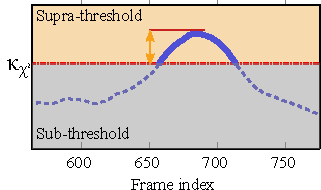
\includegraphics[width=3.5in]{gfx/Chapter05/tuning_curve-thresh.pdf}
%  \caption{Sub-threshold and supra-threshold regions can be identified by setting a threshold on the amplitude of the $\kappa_{\chi^2}$ similarity measure; the height of the threshold controls the support region of supra-threshold region of an artificial place cell.}
%  \label{fig:Supra}
%\end{figure}


 The place cell is modelled by extracting the Frame-Encoding Vector (FEV), $\mathbf{v}_{r_i}$, when the camera is at position $\ell_i$ from one or more reference journeys and calculating the supra-threshold response to some frame $\mathbf{v}_{\ell}$ acquired at location $\ell$. As $\ell$ is varied, $\kappa_{\chi^2}(\mathbf{v}_{\ell},\mathbf{v}_{r_i})$ changes accordingly.  The set of supra-thresholded response curves, $r_i(\ell)$, is generated using:
\be
r_i(\ell) = U(\kappa_{\chi^2}(\mathbf{v}_{\ell},\mathbf{v}_{r_i}) - T_i)\cdot \kappa_{\chi^2}(\mathbf{v}_{\ell},\mathbf{v}_{r_i})
\ee
where $U(\cdot)$ represents the unit step function and $T_i$ represents a suitable threshold. Curves acquired by averaging responses from several journeys with respect to the same APC location may be referred to as an APC {\em tuning curve}.

By defining APCs at regular intervals along a corridor, a simple population code for location can be devised. In Fig.~\ref{fig:APCMany}, the {\em average} response from each of several such APC cell responses is plotted along the length of one corridor.  These curves are produced by setting APCs to be spaced every 4 m within the corridor, and constructing the average APC responses.  In Fig.~\ref{fig:APCMany}, ground truth was used to register the curves for illustrative purposes.

\begin{figure}
\centering
  \setlength\figureheight{0.5\linewidth}
  \setlength\figurewidth{.9\linewidth}
  % This file was created by matlab2tikz.
% Minimal pgfplots version: 1.3
%
%The latest updates can be retrieved from
%  http://www.mathworks.com/matlabcentral/fileexchange/22022-matlab2tikz
%where you can also make suggestions and rate matlab2tikz.
%
\definecolor{mycolor1}{rgb}{0.00000,0.44700,0.74100}%
\definecolor{mycolor2}{rgb}{0.85000,0.32500,0.09800}%
\definecolor{mycolor3}{rgb}{0.92900,0.69400,0.12500}%
\definecolor{mycolor4}{rgb}{0.49400,0.18400,0.55600}%
\definecolor{mycolor5}{rgb}{0.46600,0.67400,0.18800}%
\definecolor{mycolor6}{rgb}{0.30100,0.74500,0.93300}%
\definecolor{mycolor7}{rgb}{0.63500,0.07800,0.18400}%
%
\begin{tikzpicture}

\begin{axis}[%
width=\figurewidth,
height=\figureheight,
%at={(0.758333in,0.48125in)},
scale only axis,
xmin=-1193.72122445853,
xmax=1199.71982357641,
xlabel={Ground truth in a section of corridor (cm)},
ymin=6,
ymax=16.9407386779785,
ylabel={APC Responses (A.U.)},
title style={font=\bfseries},
%title={},
axis x line*=bottom,
axis y line*=left,
legend columns=5,
/pgf/number format/1000 sep={},
legend style={legend cell align=left,align=left,at={(1.1,1.1)},draw=none},
legend style={font=\footnotesize}
]
\addplot [color=mycolor1,solid,line width=1.5pt]
  table[row sep=crcr]{%
-1193.72122445853	16.9407386779785\\
-1187.72262534064	15.6843627293905\\
-1181.72402622276	15.2515630722046\\
-1175.72542710488	14.9613719667707\\
-1169.726827987	14.5209669537014\\
-1163.72822886912	14.0880492817272\\
-1157.72962975123	13.7599135912382\\
-1151.73103063335	13.4953484217326\\
-1145.73243151547	13.1921173544491\\
-1139.73383239759	12.8910260451467\\
-1133.73523327971	12.5336408615112\\
-1127.73663416182	12.258525497035\\
-1121.73803504394	11.9852022371794\\
-1115.73943592606	11.7476778532329\\
-1109.74083680818	11.500297847547\\
-1103.7422376903	11.2994679902729\\
-1097.74363857241	11.0807148280897\\
-1091.74503945453	10.9028805682534\\
-1085.74644033665	10.7555287511725\\
-1079.74784121877	10.6352120951602\\
-1073.74924210089	10.5394358383982\\
-1067.750642983	10.4399944104646\\
-1061.75204386512	10.3081314689235\\
-1055.75344474724	10.1789315876208\\
-1049.75484562936	10.0691849056043\\
-1043.75624651148	9.99731129094174\\
-1037.75764739359	9.94793906964754\\
-1031.75904827571	9.92680163132517\\
-1025.76044915783	9.90567262549149\\
-1019.76185003995	9.89353661788137\\
-1013.76325092207	9.87450092717221\\
-1007.76465180418	9.85822687650982\\
-1001.7660526863	9.82285986448589\\
-995.767453568419	9.79963829642848\\
-989.768854450537	9.75731101788972\\
-983.770255332655	9.71796648125899\\
-977.771656214773	9.70153080789666\\
-971.773057096891	9.70624391656173\\
-965.774457979009	9.68029463918585\\
-959.775858861127	9.61910006874486\\
-953.777259743245	9.55090447476035\\
-947.778660625363	9.5083128778558\\
-941.780061507481	9.48164021341424\\
-935.781462389599	9.45037073838083\\
-929.782863271716	9.46973976336027\\
-923.784264153834	9.47496559745387\\
-917.785665035952	9.48131757033499\\
-911.78706591807	9.50782745762875\\
-905.788466800188	9.50184606250964\\
-899.789867682306	9.50906507592452\\
-893.791268564424	9.52369484148527\\
-887.792669446542	9.53914873223555\\
-881.79407032866	9.56453002126593\\
-875.795471210778	9.5490964588366\\
-869.796872092896	9.56866088666414\\
-863.798272975014	9.57917951282702\\
-857.799673857132	9.57490228351794\\
-851.80107473925	9.59033870697021\\
-845.802475621368	9.64775732943886\\
-839.803876503486	9.69510218971654\\
-833.805277385604	9.74842136784604\\
-827.806678267722	9.77508474651136\\
-821.80807914984	9.78608422530325\\
-815.809480031958	9.75724431088096\\
-809.810880914076	9.71628364763762\\
-803.812281796194	9.66527768185264\\
-797.813682678312	9.59674433657998\\
-791.81508356043	9.58135007557116\\
-785.816484442548	9.51420804073936\\
-779.817885324665	9.42849480478387\\
-773.819286206784	9.38508691285786\\
-767.820687088901	9.3195642672087\\
-761.822087971019	9.30285905536852\\
-755.823488853137	9.25530378442062\\
-749.824889735255	9.22656907533345\\
-743.826290617373	9.21548763074373\\
-737.827691499491	9.18925717002467\\
-731.829092381609	9.16857940272281\\
-725.830493263727	9.17328488199334\\
-719.831894145845	9.15506603843287\\
-713.833295027963	9.15491746601306\\
-707.834695910081	9.15044674120451\\
-701.836096792199	9.12875080108643\\
-695.837497674317	9.11097682149787\\
-689.838898556435	9.12068894034938\\
-683.840299438553	9.14774287374396\\
-677.841700320671	9.14443568179482\\
-671.843101202789	9.21245404293662\\
-665.844502084907	9.25902431889584\\
-659.845902967025	9.2796664488943\\
-653.847303849143	9.30741144481458\\
-647.848704731261	9.31202692734568\\
-641.850105613379	9.27061116067987\\
-635.851506495497	9.19576165550633\\
-629.852907377614	9.13512101926302\\
-623.854308259732	9.09386200653879\\
-617.85570914185	9.04144299657721\\
-611.857110023968	9.01009637431094\\
-605.858510906086	8.99524535630879\\
-599.859911788204	8.98515979867233\\
-593.861312670322	8.96430123479743\\
-587.86271355244	8.97450022948416\\
-581.864114434558	8.99513623588964\\
-575.865515316676	8.98986151343898\\
-569.866916198794	8.96746858797575\\
-563.868317080912	8.94336858548616\\
-557.86971796303	8.90885536294235\\
-551.871118845148	8.89461991661473\\
-545.872519727266	8.85185625678615\\
-539.873920609384	8.80509660118505\\
-533.875321491502	8.77622290661461\\
-527.87672237362	8.75422299535651\\
-521.878123255738	8.81455496737832\\
-515.879524137856	8.86164755570261\\
-509.880925019974	8.88624115994102\\
-503.882325902091	8.91184079019647\\
-497.88372678421	8.90392454046952\\
-491.885127666327	8.89473202354029\\
-485.886528548445	8.89292059446636\\
-479.887929430563	8.90409394314414\\
-473.889330312682	8.88552675749126\\
-467.890731194799	8.85545795842221\\
-461.892132076917	8.83008414820621\\
-455.893532959035	8.79158416547273\\
-449.894933841153	8.75964189830579\\
-443.896334723271	8.70555571505898\\
-437.897735605389	8.68723251945094\\
-431.899136487507	8.6613833276849\\
-425.900537369625	8.66857950310958\\
-419.901938251743	8.6453625528436\\
-413.903339133861	8.64757530312789\\
-407.904740015979	8.60468194359227\\
-401.906140898097	8.52794564397711\\
-395.907541780215	8.44520601473356\\
-389.908942662333	8.37650778419093\\
-383.910343544451	8.30070821862472\\
-377.911744426569	8.23591817052741\\
-371.913145308687	8.12273103312442\\
-365.914546190805	7.99770124335038\\
-359.915947072923	7.90073911767257\\
-353.917347955041	7.81033402995059\\
-347.918748837159	7.73379142660844\\
-341.920149719277	7.65095959211651\\
-335.921550601395	7.58865281155235\\
-329.922951483512	7.54740172938297\\
-323.92435236563	7.49370165875084\\
-317.925753247748	7.46047298531783\\
-311.927154129866	7.42358787436234\\
-305.928555011984	7.3813943862915\\
-299.929955894102	7.37833397012008\\
-293.93135677622	7.34966235411794\\
-287.932757658338	7.32545247830843\\
-281.934158540456	7.34303491993954\\
-275.935559422574	7.33658419157329\\
-269.936960304692	7.35760149202849\\
-263.93836118681	7.37448340968082\\
-257.939762068928	7.41973156678049\\
-251.941162951046	7.47752405467786\\
-245.942563833164	7.50591022089908\\
-239.943964715282	7.55859329825953\\
-233.9453655974	7.58727475216514\\
-227.946766479518	7.64949994338186\\
-221.948167361636	7.69168058194612\\
-215.949568243754	7.74136435358148\\
-209.950969125872	7.76518962257787\\
-203.952370007989	7.76904854021574\\
-197.953770890108	7.78543617850856\\
-191.955171772226	7.81279850006104\\
-185.956572654344	7.80010050221493\\
-179.957973536461	7.79538515994423\\
-173.95937441858	7.80504502748188\\
-167.960775300698	7.80355029357107\\
-161.962176182815	7.80904619317306\\
-155.963577064933	7.82351503874126\\
-149.964977947051	7.85262403990093\\
-143.966378829169	7.88298940658569\\
-137.967779711287	7.91209700233058\\
-131.969180593405	7.91953721799348\\
-125.970581475523	7.91757538444117\\
-119.971982357641	7.91943961695621\\
-113.973383239759	7.90393533204731\\
-107.974784121877	7.90795742838006\\
-101.976185003995	7.89816118541517\\
-95.9775858861126	7.87790634757594\\
-89.9789867682307	7.89164590835571\\
-83.9803876503488	7.88687934373554\\
-77.9817885324669	7.87878463142796\\
-71.9831894145846	7.87826324764051\\
-65.9845902967027	7.83595248272544\\
-59.9859911788208	7.79042979290611\\
-53.9873920609384	7.72422459251002\\
-47.9887929430565	7.65842194306223\\
-41.9901938251746	7.54167132628591\\
-35.9915947072923	7.4340863980745\\
-29.9929955894104	7.33989477157593\\
-23.9943964715285	7.22333955764771\\
-17.9957973536461	7.14914181357936\\
-11.9971982357642	7.05465299204776\\
-5.99859911788235	6.95820544895373\\
0	6.86635617205971\\
5.99859911788189	6.75687817523354\\
11.9971982357638	6.65221502906398\\
17.9957973536457	6.57854047574495\\
23.994396471528	6.50126813587389\\
29.9929955894099	6.41451122886256\\
35.9915947072918	6.33091499930934\\
41.9901938251742	6.25720410597952\\
47.9887929430561	6.21729848259374\\
53.987392060938	6.17646375455354\\
59.9859911788203	6.14741267656025\\
65.9845902967022	6.11924397317987\\
71.9831894145846	6.11924397317987\\
77.9817885324665	6.09407964505647\\
83.9803876503483	6.06438004343133\\
89.9789867682307	6.05799137918573\\
95.9775858861126	6.04077140908492\\
101.976185003994	6.03393105456704\\
107.974784121876	6.05089907897146\\
113.973383239759	6.05089907897146\\
119.971982357641	6.06171703338623\\
125.970581475523	6.08827708896838\\
131.969180593404	6.10737361406025\\
137.967779711287	6.11772471980045\\
143.966378829169	6.1163232702958\\
149.964977947051	6.14079861891897\\
155.963577064933	6.15723775562487\\
161.962176182815	6.17221782082006\\
167.960775300697	6.17400528255262\\
173.959374418579	6.17400528255262\\
179.957973536461	6.17400528255262\\
185.956572654343	6.17400528255262\\
191.955171772225	6.17400528255262\\
197.953770890107	6.17400528255262\\
203.952370007989	6.17400528255262\\
209.950969125871	6.17400528255262\\
215.949568243753	6.17362218154104\\
221.948167361636	6.15480443050987\\
227.946766479517	6.15480443050987\\
233.945365597399	6.1439864760951\\
239.943964715282	6.11742642051295\\
245.942563833164	6.0962035028558\\
251.941162951045	6.072501358233\\
257.939762068928	6.05804290269551\\
263.93836118681	6.03356755407233\\
269.936960304692	6.01676752692775\\
275.935559422574	6.00178746173256\\
281.934158540456	6\\
287.932757658338	6\\
293.93135677622	6\\
299.929955894102	6\\
305.928555011984	6\\
311.927154129866	6\\
317.925753247748	6\\
323.92435236563	6\\
329.922951483512	6\\
335.921550601394	6\\
341.920149719276	6\\
347.918748837158	6\\
353.91734795504	6\\
359.915947072922	6\\
365.914546190804	6\\
371.913145308686	6\\
377.911744426568	6\\
383.91034354445	6\\
389.908942662332	6\\
395.907541780215	6\\
401.906140898097	6\\
407.904740015978	6\\
413.903339133861	6\\
419.901938251743	6\\
425.900537369625	6\\
431.899136487507	6\\
437.897735605389	6\\
443.896334723271	6\\
449.894933841153	6\\
455.893532959035	6\\
461.892132076917	6\\
467.890731194799	6\\
473.889330312681	6\\
479.887929430563	6\\
485.886528548445	6\\
491.885127666327	6\\
497.883726784209	6\\
503.882325902091	6\\
509.880925019973	6\\
515.879524137855	6\\
521.878123255737	6\\
527.876722373619	6\\
533.875321491501	6\\
539.873920609384	6\\
545.872519727266	6\\
551.871118845148	6\\
557.86971796303	6\\
563.868317080912	6\\
569.866916198794	6\\
575.865515316676	6\\
581.864114434558	6\\
587.86271355244	6\\
593.861312670322	6\\
599.859911788204	6\\
605.858510906086	6\\
611.857110023968	6\\
617.85570914185	6\\
623.854308259732	6\\
629.852907377614	6\\
635.851506495496	6\\
641.850105613378	6\\
647.84870473126	6\\
653.847303849142	6\\
659.845902967024	6\\
665.844502084906	6\\
671.843101202789	6\\
677.84170032067	6\\
683.840299438552	6\\
689.838898556435	6\\
695.837497674317	6\\
701.836096792199	6\\
707.83469591008	6\\
713.833295027963	6\\
719.831894145845	6\\
725.830493263727	6\\
731.829092381609	6\\
737.827691499491	6\\
743.826290617373	6\\
749.824889735255	6\\
755.823488853137	6\\
761.822087971019	6\\
767.820687088901	6\\
773.819286206783	6\\
779.817885324665	6\\
785.816484442547	6\\
791.815083560429	6\\
797.813682678311	6\\
803.812281796193	6\\
809.810880914075	6\\
815.809480031957	6\\
821.808079149839	6\\
827.806678267722	6\\
833.805277385603	6\\
839.803876503485	6\\
845.802475621368	6\\
851.80107473925	6\\
857.799673857131	6\\
863.798272975014	6\\
869.796872092896	6\\
875.795471210778	6\\
881.79407032866	6\\
887.792669446542	6\\
893.791268564424	6\\
899.789867682306	6\\
905.788466800188	6\\
911.78706591807	6\\
917.785665035952	6\\
923.784264153835	6\\
929.782863271716	6\\
935.781462389598	6\\
941.78006150748	6\\
947.778660625363	6\\
953.777259743244	6\\
959.775858861126	6\\
965.774457979009	6\\
971.773057096891	6\\
977.771656214773	6\\
983.770255332655	6\\
989.768854450537	6\\
995.767453568419	6\\
1001.7660526863	6\\
1007.76465180418	6\\
1013.76325092206	6\\
1019.76185003995	6\\
1025.76044915783	6\\
1031.75904827571	6\\
1037.75764739359	6\\
1043.75624651148	6\\
1049.75484562936	6\\
1055.75344474724	6\\
1061.75204386512	6\\
1067.750642983	6\\
1073.74924210089	6\\
1079.74784121877	6\\
1085.74644033665	6\\
1091.74503945453	6\\
1097.74363857241	6\\
1103.7422376903	6\\
1109.74083680818	6\\
1115.73943592606	6\\
1121.73803504394	6\\
1127.73663416182	6\\
1133.73523327971	6\\
1139.73383239759	6\\
1145.73243151547	6\\
1151.73103063335	6\\
1157.72962975123	6\\
1163.72822886912	6\\
1169.726827987	6\\
1175.72542710488	6\\
1181.72402622276	6\\
1187.72262534064	6\\
1193.72122445853	6\\
1199.71982357641	6\\
};
\addlegendentry{APC 1};

\addplot [color=mycolor2,solid,line width=1.5pt]
  table[row sep=crcr]{%
-1193.72122445853	10.5959300994873\\
-1187.72262534064	10.8642533620199\\
-1181.72402622276	10.8549955368042\\
-1175.72542710488	10.9595305579049\\
-1169.726827987	10.9954918755425\\
-1163.72822886912	11.0506480823864\\
-1157.72962975123	11.1558049275325\\
-1151.73103063335	11.298285484314\\
-1145.73243151547	11.4625097723568\\
-1139.73383239759	11.6177242178666\\
-1133.73523327971	11.7520020635504\\
-1127.73663416182	11.8440486506412\\
-1121.73803504394	11.9493306310553\\
-1115.73943592606	12.0874268883153\\
-1109.74083680818	12.2205122395566\\
-1103.7422376903	12.3387376383731\\
-1097.74363857241	12.456448856153\\
-1091.74503945453	12.6030157992714\\
-1085.74644033665	12.7264460513466\\
-1079.74784121877	12.8868263144242\\
-1073.74924210089	13.0280915310508\\
-1067.750642983	13.1688943662141\\
-1061.75204386512	13.3251141497963\\
-1055.75344474724	13.4409471311067\\
-1049.75484562936	13.562418536136\\
-1043.75624651148	13.6738463953922\\
-1037.75764739359	13.8081390481246\\
-1031.75904827571	13.9414686403776\\
-1025.76044915783	13.9959785561813\\
-1019.76185003995	14.0634361066316\\
-1013.76325092207	14.1520124736585\\
-1007.76465180418	14.2112342934859\\
-1001.7660526863	14.2658835461265\\
-995.767453568419	14.30106253373\\
-989.768854450537	14.3545282263505\\
-983.770255332655	14.5196371580425\\
-977.771656214773	14.5223844929745\\
-971.773057096891	14.576610364412\\
-965.774457979009	14.5413101095902\\
-959.775858861127	14.4753937972219\\
-953.777259743245	14.3949344534623\\
-947.778660625363	14.2635527660972\\
-941.780061507481	14.1658490331549\\
-935.781462389599	14.0377534063239\\
-929.782863271716	13.9432240536338\\
-923.784264153834	13.8440857937461\\
-917.785665035952	13.7407114631251\\
-911.78706591807	13.6719111894306\\
-905.788466800188	13.5778514460513\\
-899.789867682306	13.4715016515631\\
-893.791268564424	13.3864849492123\\
-887.792669446542	13.2844914386147\\
-881.79407032866	13.2026746649491\\
-875.795471210778	13.0693043658608\\
-869.796872092896	12.8212226064582\\
-863.798272975014	12.7185231258995\\
-857.799673857132	12.5866358405665\\
-851.80107473925	12.5037210364091\\
-845.802475621368	12.4337277161448\\
-839.803876503486	12.3621282577515\\
-833.805277385604	12.3058032487568\\
-827.806678267722	12.2180296245374\\
-821.80807914984	12.1631642893741\\
-815.809480031958	12.0487607152838\\
-809.810880914076	11.9109998000296\\
-803.812281796194	11.752385741786\\
-797.813682678312	11.5845127607647\\
-791.81508356043	11.4602006611071\\
-785.816484442548	11.3088475277549\\
-779.817885324665	11.1382745943571\\
-773.819286206784	10.9879253788998\\
-767.820687088901	10.8385585483752\\
-761.822087971019	10.7306927630776\\
-755.823488853137	10.6608379263627\\
-749.824889735255	10.5802076239335\\
-743.826290617373	10.5200664118717\\
-737.827691499491	10.4470687665437\\
-731.829092381609	10.4238930752403\\
-725.830493263727	10.4147043228149\\
-719.831894145845	10.3819344671149\\
-713.833295027963	10.3697790346648\\
-707.834695910081	10.3384467175132\\
-701.836096792199	10.3081651988782\\
-695.837497674317	10.2655706907573\\
-689.838898556435	10.3067157644975\\
-683.840299438553	10.3698602475618\\
-677.841700320671	10.4066724777222\\
-671.843101202789	10.4507615942704\\
-665.844502084907	10.4823688707854\\
-659.845902967025	10.4857632988378\\
-653.847303849143	10.4964280379446\\
-647.848704731261	10.4712521402459\\
-641.850105613379	10.3777767984491\\
-635.851506495497	10.2770225123355\\
-629.852907377614	10.1680652216861\\
-623.854308259732	10.0558867705496\\
-617.85570914185	9.92862841957494\\
-611.857110023968	9.81038033334832\\
-605.858510906086	9.72548911446019\\
-599.859911788204	9.64266224911338\\
-593.861312670322	9.56064987182617\\
-587.86271355244	9.51463844901637\\
-581.864114434558	9.47864532470703\\
-575.865515316676	9.38163576628032\\
-569.866916198794	9.27680105912058\\
-563.868317080912	9.18141791695043\\
-557.86971796303	9.13133174494693\\
-551.871118845148	9.07718251880847\\
-545.872519727266	9.02782088831851\\
-539.873920609384	8.9667117972123\\
-533.875321491502	8.92358779907227\\
-527.87672237362	8.88514051939311\\
-521.878123255738	8.96021556854248\\
-515.879524137856	9.02303198764199\\
-509.880925019974	9.06523493716591\\
-503.882325902091	9.1101612291838\\
-497.88372678421	9.13475006505063\\
-491.885127666327	9.13907081202457\\
-485.886528548445	9.15454894617984\\
-479.887929430563	9.15093532361482\\
-473.889330312682	9.16183878246107\\
-467.890731194799	9.19166063007556\\
-461.892132076917	9.22614980998792\\
-455.893532959035	9.21716268439042\\
-449.894933841153	9.19537589424535\\
-443.896334723271	9.15523900483784\\
-437.897735605389	9.16704177856445\\
-431.899136487507	9.1766723833586\\
-425.900537369625	9.18770488939787\\
-419.901938251743	9.18758030941612\\
-413.903339133861	9.18286514282227\\
-407.904740015979	9.09285505194413\\
-401.906140898097	9.01827370493035\\
-395.907541780215	8.94846238588032\\
-389.908942662333	8.8841643584402\\
-383.910343544451	8.8377564580817\\
-377.911744426569	8.79279703842966\\
-371.913145308687	8.68411425540322\\
-365.914546190805	8.62206938392238\\
-359.915947072923	8.52401853862562\\
-353.917347955041	8.42960568478233\\
-347.918748837159	8.3485978277106\\
-341.920149719277	8.28232112683748\\
-335.921550601395	8.21981384879664\\
-329.922951483512	8.17093736247012\\
-323.92435236563	8.11494714335391\\
-317.925753247748	8.0805825434233\\
-311.927154129866	8.05678104099474\\
-305.928555011984	8.03240306753861\\
-299.929955894102	8.03184755224931\\
-293.93135677622	8.0263792841058\\
-287.932757658338	7.98695483960604\\
-281.934158540456	7.97557529650237\\
-275.935559422574	7.948966201983\\
-269.936960304692	7.9107332982515\\
-263.93836118681	7.88126330626638\\
-257.939762068928	7.89695355766698\\
-251.941162951046	7.89590318579423\\
-245.942563833164	7.89659698385941\\
-239.943964715282	7.90061767477738\\
-233.9453655974	7.88528909181294\\
-227.946766479518	7.89879211626555\\
-221.948167361636	7.92523961318167\\
-215.949568243754	7.95964057821976\\
-209.950969125872	7.93895791706286\\
-203.952370007989	7.88826390316612\\
-197.953770890108	7.84663913124486\\
-191.955171772226	7.82073417462801\\
-185.956572654344	7.77641735578838\\
-179.957973536461	7.72762943568983\\
-173.95937441858	7.69990120436016\\
-167.960775300698	7.68469040017379\\
-161.962176182815	7.66964031520643\\
-155.963577064933	7.66318921038979\\
-149.964977947051	7.66165289125944\\
-143.966378829169	7.68134945317319\\
-137.967779711287	7.69044755634509\\
-131.969180593405	7.67296532580727\\
-125.970581475523	7.63166490354036\\
-119.971982357641	7.59821103748522\\
-113.973383239759	7.55744238903648\\
-107.974784121877	7.51892709732055\\
-101.976185003995	7.47660137477674\\
-95.9775858861126	7.45843473233675\\
-89.9789867682307	7.46664488943\\
-83.9803876503488	7.47586930425543\\
-77.9817885324669	7.46852867226852\\
-71.9831894145846	7.49384777169479\\
-65.9845902967027	7.47364669097097\\
-59.9859911788208	7.48388774771439\\
-53.9873920609384	7.45975552107158\\
-47.9887929430565	7.42651841514989\\
-41.9901938251746	7.39207646721288\\
-35.9915947072923	7.34691210796958\\
-29.9929955894104	7.30491540306493\\
-23.9943964715285	7.26741642700998\\
-17.9957973536461	7.24558624468352\\
-11.9971982357642	7.2351057403966\\
-5.99859911788235	7.22886379141556\\
0	7.19403008410805\\
5.99859911788189	7.12627724597328\\
11.9971982357638	7.09900805824681\\
17.9957973536457	7.0660380313271\\
23.994396471528	7.03709205828215\\
29.9929955894099	6.99075445375945\\
35.9915947072918	6.95262015493293\\
41.9901938251742	6.91095972061157\\
47.9887929430561	6.88293906262046\\
53.987392060938	6.81904634676482\\
59.9859911788203	6.78104448318481\\
65.9845902967022	6.75447393718519\\
71.9831894145846	6.74182470221268\\
77.9817885324665	6.71269005223324\\
83.9803876503483	6.67771540190044\\
89.9789867682307	6.6341999957436\\
95.9775858861126	6.60747317263955\\
101.976185003994	6.57227265207391\\
107.974784121876	6.5648223475406\\
113.973383239759	6.56288551029406\\
119.971982357641	6.57599366338629\\
125.970581475523	6.55409095161839\\
131.969180593404	6.54273105922498\\
137.967779711287	6.51757318095157\\
143.966378829169	6.49310777061864\\
149.964977947051	6.47475087015252\\
155.963577064933	6.44793593256097\\
161.962176182815	6.43817186355591\\
167.960775300697	6.45059045992399\\
173.959374418579	6.44071393263967\\
179.957973536461	6.45182973460147\\
185.956572654343	6.44016052547254\\
191.955171772225	6.44438572933799\\
197.953770890107	6.42789009997719\\
203.952370007989	6.43300528275339\\
209.950969125871	6.41946463835867\\
215.949568243753	6.40616959019711\\
221.948167361636	6.36516330116674\\
227.946766479517	6.3387259433144\\
233.945365597399	6.32304879238731\\
239.943964715282	6.29323969389263\\
245.942563833164	6.27923001741108\\
251.941162951045	6.25022825441862\\
257.939762068928	6.22586172505429\\
263.93836118681	6.20280950947812\\
269.936960304692	6.18816373222753\\
275.935559422574	6.17901643953825\\
281.934158540456	6.15450073543348\\
287.932757658338	6.14413728212055\\
293.93135677622	6.120748394414\\
299.929955894102	6.09286330875598\\
305.928555011984	6.07197485472027\\
311.927154129866	6.06317118594521\\
317.925753247748	6.04102960385774\\
323.92435236563	6.02611371090538\\
329.922951483512	6.01825026461953\\
335.921550601394	6.01214865634316\\
341.920149719276	6.01214865634316\\
347.918748837158	6.01214865634316\\
353.91734795504	6.01214865634316\\
359.915947072922	6\\
365.914546190804	6.00564705698114\\
371.913145308686	6.00564705698114\\
377.911744426568	6.00564705698114\\
383.91034354445	6.00564705698114\\
389.908942662332	6.00564705698114\\
395.907541780215	6.00564705698114\\
401.906140898097	6.00564705698114\\
407.904740015978	6.00564705698114\\
413.903339133861	6.00564705698114\\
419.901938251743	6.00564705698114\\
425.900537369625	6.00564705698114\\
431.899136487507	6.00564705698114\\
437.897735605389	6.00564705698114\\
443.896334723271	6.00564705698114\\
449.894933841153	6.00564705698114\\
455.893532959035	6.00564705698114\\
461.892132076917	6.00564705698114\\
467.890731194799	6.00564705698114\\
473.889330312681	6.00564705698114\\
479.887929430563	6\\
485.886528548445	6\\
491.885127666327	6\\
497.883726784209	6\\
503.882325902091	6\\
509.880925019973	6\\
515.879524137855	6\\
521.878123255737	6\\
527.876722373619	6\\
533.875321491501	6\\
539.873920609384	6\\
545.872519727266	6\\
551.871118845148	6\\
557.86971796303	6\\
563.868317080912	6\\
569.866916198794	6\\
575.865515316676	6\\
581.864114434558	6\\
587.86271355244	6\\
593.861312670322	6\\
599.859911788204	6\\
605.858510906086	6\\
611.857110023968	6\\
617.85570914185	6\\
623.854308259732	6\\
629.852907377614	6\\
635.851506495496	6\\
641.850105613378	6\\
647.84870473126	6\\
653.847303849142	6\\
659.845902967024	6\\
665.844502084906	6\\
671.843101202789	6\\
677.84170032067	6\\
683.840299438552	6\\
689.838898556435	6\\
695.837497674317	6\\
701.836096792199	6\\
707.83469591008	6\\
713.833295027963	6\\
719.831894145845	6\\
725.830493263727	6\\
731.829092381609	6\\
737.827691499491	6\\
743.826290617373	6\\
749.824889735255	6\\
755.823488853137	6\\
761.822087971019	6\\
767.820687088901	6\\
773.819286206783	6\\
779.817885324665	6\\
785.816484442547	6\\
791.815083560429	6\\
797.813682678311	6\\
803.812281796193	6\\
809.810880914075	6\\
815.809480031957	6\\
821.808079149839	6\\
827.806678267722	6\\
833.805277385603	6\\
839.803876503485	6\\
845.802475621368	6\\
851.80107473925	6\\
857.799673857131	6\\
863.798272975014	6\\
869.796872092896	6\\
875.795471210778	6\\
881.79407032866	6\\
887.792669446542	6\\
893.791268564424	6\\
899.789867682306	6\\
905.788466800188	6\\
911.78706591807	6\\
917.785665035952	6\\
923.784264153835	6\\
929.782863271716	6\\
935.781462389598	6\\
941.78006150748	6\\
947.778660625363	6\\
953.777259743244	6\\
959.775858861126	6\\
965.774457979009	6\\
971.773057096891	6\\
977.771656214773	6\\
983.770255332655	6\\
989.768854450537	6\\
995.767453568419	6\\
1001.7660526863	6\\
1007.76465180418	6\\
1013.76325092206	6\\
1019.76185003995	6\\
1025.76044915783	6\\
1031.75904827571	6\\
1037.75764739359	6\\
1043.75624651148	6\\
1049.75484562936	6\\
1055.75344474724	6\\
1061.75204386512	6\\
1067.750642983	6\\
1073.74924210089	6\\
1079.74784121877	6\\
1085.74644033665	6\\
1091.74503945453	6\\
1097.74363857241	6\\
1103.7422376903	6\\
1109.74083680818	6\\
1115.73943592606	6\\
1121.73803504394	6\\
1127.73663416182	6\\
1133.73523327971	6\\
1139.73383239759	6\\
1145.73243151547	6\\
1151.73103063335	6\\
1157.72962975123	6\\
1163.72822886912	6\\
1169.726827987	6\\
1175.72542710488	6\\
1181.72402622276	6\\
1187.72262534064	6\\
1193.72122445853	6\\
1199.71982357641	6\\
};
\addlegendentry{APC 2};

\addplot [color=mycolor3,solid,line width=1.5pt]
  table[row sep=crcr]{%
-1193.72122445853	9.74725532531738\\
-1187.72262534064	9.95132605234782\\
-1181.72402622276	10.0572641372681\\
-1175.72542710488	10.0742365973336\\
-1169.726827987	10.1245347128974\\
-1163.72822886912	10.1510334881869\\
-1157.72962975123	10.2141499886146\\
-1151.73103063335	10.327562268575\\
-1145.73243151547	10.4085612016566\\
-1139.73383239759	10.4738598873741\\
-1133.73523327971	10.529874701249\\
-1127.73663416182	10.5674936394942\\
-1121.73803504394	10.6158335334376\\
-1115.73943592606	10.6893445065147\\
-1109.74083680818	10.7354532542982\\
-1103.7422376903	10.7816080796091\\
-1097.74363857241	10.8207583678396\\
-1091.74503945453	10.8540007440667\\
-1085.74644033665	10.8759942807649\\
-1079.74784121877	10.8868980909649\\
-1073.74924210089	10.9362259413067\\
-1067.750642983	10.9612961317364\\
-1061.75204386512	10.9588043313277\\
-1055.75344474724	10.9167049307572\\
-1049.75484562936	10.9087832099513\\
-1043.75624651148	10.9145177038092\\
-1037.75764739359	10.9274671454179\\
-1031.75904827571	10.9498720169067\\
-1025.76044915783	10.9221296310425\\
-1019.76185003995	10.9020567442241\\
-1013.76325092207	10.8953986418875\\
-1007.76465180418	10.8518733978271\\
-1001.7660526863	10.7910719921714\\
-995.767453568419	10.729878927532\\
-989.768854450537	10.6871579320807\\
-983.770255332655	10.6550346675672\\
-977.771656214773	10.6310970406783\\
-971.773057096891	10.6345779519332\\
-965.774457979009	10.6084469745034\\
-959.775858861127	10.5631817265561\\
-953.777259743245	10.5044949180201\\
-947.778660625363	10.4604705509387\\
-941.780061507481	10.4554624557495\\
-935.781462389599	10.4193955471641\\
-929.782863271716	10.4379083231876\\
-923.784264153834	10.4664695639359\\
-917.785665035952	10.4834638394808\\
-911.78706591807	10.5707031049226\\
-905.788466800188	10.6355060778166\\
-899.789867682306	10.6690950393677\\
-893.791268564424	10.7923711475573\\
-887.792669446542	10.9066994817633\\
-881.79407032866	11.0557875382273\\
-875.795471210778	11.1921001735486\\
-869.796872092896	11.3700332139668\\
-863.798272975014	11.5444978914763\\
-857.799673857132	11.7000200371993\\
-851.80107473925	11.8863768828543\\
-845.802475621368	12.1103439832989\\
-839.803876503486	12.3392675299394\\
-833.805277385604	12.5765101784154\\
-827.806678267722	12.7876524674265\\
-821.80807914984	12.9927809363917\\
-815.809480031958	13.1516089690359\\
-809.810880914076	13.2959657970228\\
-803.812281796194	13.4252898065667\\
-797.813682678312	13.545348368193\\
-791.81508356043	13.7084412825735\\
-785.816484442548	13.846685811093\\
-779.817885324665	13.9145742717542\\
-773.819286206784	13.9954379232306\\
-767.820687088901	14.0630082582173\\
-761.822087971019	14.2021320744565\\
-755.823488853137	14.3319101835552\\
-749.824889735255	14.4608075995194\\
-743.826290617373	14.6012170189305\\
-737.827691499491	14.736332943565\\
-731.829092381609	14.8564080188149\\
-725.830493263727	14.9850382553904\\
-719.831894145845	15.0894981685438\\
-713.833295027963	15.2911060232865\\
-707.834695910081	15.376281186154\\
-701.836096792199	15.4024610519409\\
-695.837497674317	15.4079949730321\\
-689.838898556435	15.450173930118\\
-683.840299438553	15.4635388725682\\
-677.841700320671	15.4726408406308\\
-671.843101202789	15.4863637623034\\
-665.844502084907	15.4844580198589\\
-659.845902967025	15.4405099467227\\
-653.847303849143	15.3919080433093\\
-647.848704731261	15.2724230414943\\
-641.850105613379	15.0476124412135\\
-635.851506495497	14.7875182503148\\
-629.852907377614	14.5551619780691\\
-623.854308259732	14.3205370652048\\
-617.85570914185	14.0814091531854\\
-611.857110023968	13.8402305904188\\
-605.858510906086	13.6313678339908\\
-599.859911788204	13.328567002949\\
-593.861312670322	13.1132206163908\\
-587.86271355244	12.9356001301816\\
-581.864114434558	12.7817306016621\\
-575.865515316676	12.5829910479094\\
-569.866916198794	12.3978419052927\\
-563.868317080912	12.2088665209318\\
-557.86971796303	12.0625728807951\\
-551.871118845148	11.911691866423\\
-545.872519727266	11.7649913587068\\
-539.873920609384	11.6141958236694\\
-533.875321491502	11.4881274072747\\
-527.87672237362	11.3910715203536\\
-521.878123255738	11.383292700115\\
-515.879524137856	11.3498268629375\\
-509.880925019974	11.2963508304797\\
-503.882325902091	11.2325241691188\\
-497.88372678421	11.1527215054161\\
-491.885127666327	11.0648907611245\\
-485.886528548445	10.987593801398\\
-479.887929430563	10.9222498441997\\
-473.889330312682	10.8511847445839\\
-467.890731194799	10.7854571593435\\
-461.892132076917	10.7340694226717\\
-455.893532959035	10.7032638349031\\
-449.894933841153	10.6371907685932\\
-443.896334723271	10.5524405931172\\
-437.897735605389	10.4843430770071\\
-431.899136487507	10.4486270703767\\
-425.900537369625	10.4124725743344\\
-419.901938251743	10.3472125404759\\
-413.903339133861	10.3127989518015\\
-407.904740015979	10.2538302070216\\
-401.906140898097	10.1687367087916\\
-395.907541780215	10.0701662866693\\
-389.908942662333	10.0077268700851\\
-383.910343544451	9.97362432981792\\
-377.911744426569	9.93511400724712\\
-371.913145308687	9.85385387822201\\
-365.914546190805	9.76483872062282\\
-359.915947072923	9.71348958266409\\
-353.917347955041	9.65009799756502\\
-347.918748837159	9.60709150213944\\
-341.920149719277	9.53823661804199\\
-335.921550601395	9.46687954350521\\
-329.922951483512	9.41589812228554\\
-323.92435236563	9.41684778113114\\
-317.925753247748	9.40903653596577\\
-311.927154129866	9.41944890273245\\
-305.928555011984	9.40227930169356\\
-299.929955894102	9.42208766937256\\
-293.93135677622	9.40965577175742\\
-287.932757658338	9.39575626975611\\
-281.934158540456	9.39502851586593\\
-275.935559422574	9.35682592893902\\
-269.936960304692	9.31763453232614\\
-263.93836118681	9.28011131286621\\
-257.939762068928	9.26451733237819\\
-251.941162951046	9.28487371143542\\
-245.942563833164	9.26151943206787\\
-239.943964715282	9.24142205087762\\
-233.9453655974	9.18746867932771\\
-227.946766479518	9.14866025824296\\
-221.948167361636	9.13431855251915\\
-215.949568243754	9.10987362108733\\
-209.950969125872	9.00843218753212\\
-203.952370007989	8.88425199609054\\
-197.953770890108	8.78260534688046\\
-191.955171772226	8.70425384923031\\
-185.956572654344	8.57539598565353\\
-179.957973536461	8.44357716409784\\
-173.95937441858	8.34182603735673\\
-167.960775300698	8.27035130952534\\
-161.962176182815	8.20151585026791\\
-155.963577064933	8.11978957527562\\
-149.964977947051	8.05541743730244\\
-143.966378829169	8.00687016938862\\
-137.967779711287	7.93048231225265\\
-131.969180593405	7.85372317464728\\
-125.970581475523	7.7819208847849\\
-119.971982357641	7.71662129853901\\
-113.973383239759	7.65493443137721\\
-107.974784121877	7.61289629183317\\
-101.976185003995	7.57437585529528\\
-95.9775858861126	7.55378542448345\\
-89.9789867682307	7.55825524581106\\
-83.9803876503488	7.54352978656166\\
-77.9817885324669	7.51939896533364\\
-71.9831894145846	7.53720644900673\\
-65.9845902967027	7.49702749754253\\
-59.9859911788208	7.48111990878456\\
-53.9873920609384	7.42199295445492\\
-47.9887929430565	7.37874891883449\\
-41.9901938251746	7.30669159638254\\
-35.9915947072923	7.23654252604434\\
-29.9929955894104	7.19029361323306\\
-23.9943964715285	7.13402805830303\\
-17.9957973536461	7.12007464860615\\
-11.9971982357642	7.10084335427535\\
-5.99859911788235	7.08239347056339\\
0	7.03718795274433\\
5.99859911788189	6.94980957633571\\
11.9971982357638	6.91212074380172\\
17.9957973536457	6.88583456842523\\
23.994396471528	6.88045619663439\\
29.9929955894099	6.84326174384669\\
35.9915947072918	6.80472298672325\\
41.9901938251742	6.77651161896555\\
47.9887929430561	6.7891078999168\\
53.987392060938	6.74883704436453\\
59.9859911788203	6.74823166194715\\
65.9845902967022	6.74499970988223\\
71.9831894145846	6.76657531135961\\
77.9817885324665	6.76123360583657\\
83.9803876503483	6.7273746289705\\
89.9789867682307	6.71792261224044\\
95.9775858861126	6.69805190437719\\
101.976185003994	6.6626286004719\\
107.974784121876	6.66872938055741\\
113.973383239759	6.67525426965011\\
119.971982357641	6.7093922966405\\
125.970581475523	6.69561521630538\\
131.969180593404	6.69561940745303\\
137.967779711287	6.6629500891033\\
143.966378829169	6.63092374801636\\
149.964977947051	6.62848053480449\\
155.963577064933	6.59257073151438\\
161.962176182815	6.56368024725663\\
167.960775300697	6.55991524144223\\
173.959374418579	6.56512624339053\\
179.957973536461	6.53391398881611\\
185.956572654343	6.51885963741102\\
191.955171772225	6.50530744853773\\
197.953770890107	6.49793042634663\\
203.952370007989	6.47851785860564\\
209.950969125871	6.43954791520771\\
215.949568243753	6.41473353536506\\
221.948167361636	6.36325743323878\\
227.946766479517	6.33027465719926\\
233.945365597399	6.29613663020887\\
239.943964715282	6.26436481977764\\
245.942563833164	6.22167552144904\\
251.941162951045	6.18969646253084\\
257.939762068928	6.17105875517193\\
263.93836118681	6.14462034325851\\
269.936960304692	6.12720745488217\\
275.935559422574	6.11527621118646\\
281.934158540456	6.09451748195448\\
287.932757658338	6.05938931515342\\
293.93135677622	6.05417961823313\\
299.929955894102	6.03093403264096\\
305.928555011984	6.02259984769319\\
311.927154129866	6.00900233419318\\
317.925753247748	6.00136265001799\\
323.92435236563	6\\
329.922951483512	6\\
335.921550601394	6\\
341.920149719276	6\\
347.918748837158	6\\
353.91734795504	6\\
359.915947072922	6\\
365.914546190804	6\\
371.913145308686	6\\
377.911744426568	6\\
383.91034354445	6\\
389.908942662332	6\\
395.907541780215	6\\
401.906140898097	6\\
407.904740015978	6\\
413.903339133861	6\\
419.901938251743	6\\
425.900537369625	6\\
431.899136487507	6\\
437.897735605389	6\\
443.896334723271	6\\
449.894933841153	6\\
455.893532959035	6\\
461.892132076917	6\\
467.890731194799	6\\
473.889330312681	6\\
479.887929430563	6\\
485.886528548445	6\\
491.885127666327	6\\
497.883726784209	6\\
503.882325902091	6\\
509.880925019973	6\\
515.879524137855	6\\
521.878123255737	6\\
527.876722373619	6\\
533.875321491501	6\\
539.873920609384	6\\
545.872519727266	6\\
551.871118845148	6\\
557.86971796303	6\\
563.868317080912	6\\
569.866916198794	6\\
575.865515316676	6\\
581.864114434558	6\\
587.86271355244	6\\
593.861312670322	6\\
599.859911788204	6\\
605.858510906086	6\\
611.857110023968	6\\
617.85570914185	6\\
623.854308259732	6\\
629.852907377614	6\\
635.851506495496	6\\
641.850105613378	6\\
647.84870473126	6\\
653.847303849142	6\\
659.845902967024	6\\
665.844502084906	6\\
671.843101202789	6\\
677.84170032067	6\\
683.840299438552	6\\
689.838898556435	6\\
695.837497674317	6\\
701.836096792199	6\\
707.83469591008	6\\
713.833295027963	6\\
719.831894145845	6\\
725.830493263727	6\\
731.829092381609	6\\
737.827691499491	6\\
743.826290617373	6\\
749.824889735255	6\\
755.823488853137	6\\
761.822087971019	6\\
767.820687088901	6\\
773.819286206783	6\\
779.817885324665	6\\
785.816484442547	6\\
791.815083560429	6\\
797.813682678311	6\\
803.812281796193	6\\
809.810880914075	6\\
815.809480031957	6\\
821.808079149839	6\\
827.806678267722	6\\
833.805277385603	6\\
839.803876503485	6\\
845.802475621368	6\\
851.80107473925	6\\
857.799673857131	6\\
863.798272975014	6\\
869.796872092896	6\\
875.795471210778	6\\
881.79407032866	6\\
887.792669446542	6\\
893.791268564424	6\\
899.789867682306	6\\
905.788466800188	6\\
911.78706591807	6\\
917.785665035952	6\\
923.784264153835	6\\
929.782863271716	6\\
935.781462389598	6\\
941.78006150748	6\\
947.778660625363	6\\
953.777259743244	6\\
959.775858861126	6\\
965.774457979009	6\\
971.773057096891	6\\
977.771656214773	6\\
983.770255332655	6\\
989.768854450537	6\\
995.767453568419	6\\
1001.7660526863	6\\
1007.76465180418	6\\
1013.76325092206	6\\
1019.76185003995	6\\
1025.76044915783	6\\
1031.75904827571	6\\
1037.75764739359	6\\
1043.75624651148	6\\
1049.75484562936	6\\
1055.75344474724	6\\
1061.75204386512	6\\
1067.750642983	6\\
1073.74924210089	6\\
1079.74784121877	6\\
1085.74644033665	6\\
1091.74503945453	6\\
1097.74363857241	6\\
1103.7422376903	6\\
1109.74083680818	6\\
1115.73943592606	6\\
1121.73803504394	6\\
1127.73663416182	6\\
1133.73523327971	6\\
1139.73383239759	6\\
1145.73243151547	6\\
1151.73103063335	6\\
1157.72962975123	6\\
1163.72822886912	6\\
1169.726827987	6\\
1175.72542710488	6\\
1181.72402622276	6\\
1187.72262534064	6\\
1193.72122445853	6\\
1199.71982357641	6\\
};
\addlegendentry{APC 3};

\addplot [color=mycolor4,solid,line width=1.5pt]
  table[row sep=crcr]{%
-1193.72122445853	8.83436012268066\\
-1187.72262534064	8.84814771016439\\
-1181.72402622276	8.88847579956055\\
-1175.72542710488	8.88921056474958\\
-1169.726827987	8.88932450612386\\
-1163.72822886912	8.89916376634078\\
-1157.72962975123	8.93232477628268\\
-1151.73103063335	8.98870913187663\\
-1145.73243151547	9.01316564223346\\
-1139.73383239759	9.00807380676269\\
-1133.73523327971	8.99861079768131\\
-1127.73663416182	8.99321541033293\\
-1121.73803504394	9.01881152705142\\
-1115.73943592606	9.02301697981985\\
-1109.74083680818	9.03187084197998\\
-1103.7422376903	9.06941594575581\\
-1097.74363857241	9.06056599867971\\
-1091.74503945453	9.07388983274761\\
-1085.74644033665	9.0845163746884\\
-1079.74784121877	9.0902607566432\\
-1073.74924210089	9.10379108629729\\
-1067.750642983	9.1007147337261\\
-1061.75204386512	9.0983348645662\\
-1055.75344474724	9.06805987107126\\
-1049.75484562936	9.05055658440841\\
-1043.75624651148	9.06275749206543\\
-1037.75764739359	9.07138819443552\\
-1031.75904827571	9.0946233147069\\
-1025.76044915783	9.1115238290084\\
-1019.76185003995	9.1448624761481\\
-1013.76325092207	9.16795956461053\\
-1007.76465180418	9.16883448550576\\
-1001.7660526863	9.16530388279965\\
-995.767453568419	9.15425109863281\\
-989.768854450537	9.11931068018863\\
-983.770255332655	9.13265032517283\\
-977.771656214773	9.12145067516126\\
-971.773057096891	9.11713304017719\\
-965.774457979009	9.09223616750617\\
-959.775858861127	9.05802390449925\\
-953.777259743245	9.02770077554803\\
-947.778660625363	8.99196348692242\\
-941.780061507481	8.9612700813695\\
-935.781462389599	8.92274334556178\\
-929.782863271716	8.89965714906391\\
-923.784264153834	8.87263438576146\\
-917.785665035952	8.83981473822342\\
-911.78706591807	8.83436714975457\\
-905.788466800188	8.80801241021407\\
-899.789867682306	8.77866268157959\\
-893.791268564424	8.75986646351061\\
-887.792669446542	8.75555590579384\\
-881.79407032866	8.77488537838585\\
-875.795471210778	8.78642980675948\\
-869.796872092896	8.79977221237986\\
-863.798272975014	8.81915052313554\\
-857.799673857132	8.83062714024594\\
-851.80107473925	8.86030126872816\\
-845.802475621368	8.91836352097361\\
-839.803876503486	8.95424797660426\\
-833.805277385604	9.02337746871145\\
-827.806678267722	9.09770553990414\\
-821.80807914984	9.18575146323756\\
-815.809480031958	9.21502213729055\\
-809.810880914076	9.2298822904888\\
-803.812281796194	9.25725665845369\\
-797.813682678312	9.26768799831993\\
-791.81508356043	9.31450392070569\\
-785.816484442548	9.35531310031289\\
-779.817885324665	9.35249991165964\\
-773.819286206784	9.39321728756553\\
-767.820687088901	9.42147074247661\\
-761.822087971019	9.48082301491185\\
-755.823488853137	9.55658501072934\\
-749.824889735255	9.64553275861238\\
-743.826290617373	9.75300547951146\\
-737.827691499491	9.85727877365916\\
-731.829092381609	9.96249891582288\\
-725.830493263727	10.0949820970234\\
-719.831894145845	10.1964891333329\\
-713.833295027963	10.2637578060752\\
-707.834695910081	10.3407027093988\\
-701.836096792199	10.4355020021137\\
-695.837497674317	10.5413038354171\\
-689.838898556435	10.6610455763967\\
-683.840299438553	10.7776575590435\\
-677.841700320671	10.8944952613429\\
-671.843101202789	11.0329539148431\\
-665.844502084907	11.1603681664718\\
-659.845902967025	11.2509642651207\\
-653.847303849143	11.3496232283743\\
-647.848704731261	11.4460107903731\\
-641.850105613379	11.4439856378656\\
-635.851506495497	11.4306708888004\\
-629.852907377614	11.4487254996049\\
-623.854308259732	11.502294640792\\
-617.85570914185	11.5281215466951\\
-611.857110023968	11.5513475317704\\
-605.858510906086	11.6005211880333\\
-599.859911788204	11.7068002600419\\
-593.861312670322	11.758054030569\\
-587.86271355244	11.8515530134502\\
-581.864114434558	11.9490205865157\\
-575.865515316676	12.0117499702855\\
-569.866916198794	12.0852875960501\\
-563.868317080912	12.1614787453099\\
-557.86971796303	12.2443685531616\\
-551.871118845148	12.3620615507427\\
-545.872519727266	12.4552620837563\\
-539.873920609384	12.5113317590011\\
-533.875321491502	12.5800365648772\\
-527.87672237362	12.6997664100245\\
-521.878123255738	12.8876661501433\\
-515.879524137856	13.0101078434994\\
-509.880925019974	13.1392345428467\\
-503.882325902091	13.2539866598029\\
-497.88372678421	13.393239774202\\
-491.885127666327	13.5300505788703\\
-485.886528548445	13.6496095657349\\
-479.887929430563	13.7856485467208\\
-473.889330312682	13.9101680454455\\
-467.890731194799	14.0151702981246\\
-461.892132076917	14.1654163159822\\
-455.893532959035	14.3096872128938\\
-449.894933841153	14.5109373393812\\
-443.896334723271	14.5808424196745\\
-437.897735605389	14.6446595944856\\
-431.899136487507	14.6970784036737\\
-425.900537369625	14.7816971226742\\
-419.901938251743	14.7964757618151\\
-413.903339133861	14.8066219028674\\
-407.904740015979	14.7635141673841\\
-401.906140898097	14.7213054958143\\
-395.907541780215	14.6072225570679\\
-389.908942662333	14.5077565343756\\
-383.910343544451	14.4039958150763\\
-377.911744426569	14.2708949038857\\
-371.913145308687	14.0815541116815\\
-365.914546190805	13.8813250190333\\
-359.915947072923	13.6762042798494\\
-353.917347955041	13.4940354196649\\
-347.918748837159	13.2699004725406\\
-341.920149719277	13.0221610822176\\
-335.921550601395	12.6921704944811\\
-329.922951483512	12.4829751064903\\
-323.92435236563	12.2958916111996\\
-317.925753247748	12.1368085459659\\
-311.927154129866	11.9752655531231\\
-305.928555011984	11.8334406300595\\
-299.929955894102	11.7205143978721\\
-293.93135677622	11.599009513855\\
-287.932757658338	11.489773599725\\
-281.934158540456	11.4104357267681\\
-275.935559422574	11.3300490128367\\
-269.936960304692	11.2363143720125\\
-263.93836118681	11.1489634262888\\
-257.939762068928	11.1036764446058\\
-251.941162951046	11.0938992751272\\
-245.942563833164	11.0227099468834\\
-239.943964715282	10.982496562757\\
-233.9453655974	10.9447948054263\\
-227.946766479518	10.9501560612729\\
-221.948167361636	10.9469661712646\\
-215.949568243754	10.9356380261873\\
-209.950969125872	10.8923317758661\\
-203.952370007989	10.8337665357088\\
-197.953770890108	10.8036400142469\\
-191.955171772226	10.7718357788889\\
-185.956572654344	10.6942691802979\\
-179.957973536461	10.6041569458811\\
-173.95937441858	10.5486178649099\\
-167.960775300698	10.4852843535574\\
-161.962176182815	10.4404924292313\\
-155.963577064933	10.3922529220581\\
-149.964977947051	10.3563322268034\\
-143.966378829169	10.3385672820242\\
-137.967779711287	10.3039422788118\\
-131.969180593405	10.2753670843024\\
-125.970581475523	10.2194419158132\\
-119.971982357641	10.1415617089523\\
-113.973383239759	10.0641323892694\\
-107.974784121877	9.99419573733681\\
-101.976185003995	9.92698709588302\\
-95.9775858861126	9.84943274447792\\
-89.9789867682307	9.81414323104055\\
-83.9803876503488	9.73259810397499\\
-77.9817885324669	9.64267605229428\\
-71.9831894145846	9.60857642324347\\
-65.9845902967027	9.55859390058015\\
-59.9859911788208	9.4843000110827\\
-53.9873920609384	9.41385048314145\\
-47.9887929430565	9.30559564891614\\
-41.9901938251746	9.18703249881142\\
-35.9915947072923	9.06420647470575\\
-29.9929955894104	8.94240710609837\\
-23.9943964715285	8.80778109399896\\
-17.9957973536461	8.71379669089066\\
-11.9971982357642	8.62557689767135\\
-5.99859911788235	8.55791250028108\\
0	8.46080212844046\\
5.99859911788189	8.31254655436466\\
11.9971982357638	8.18701924775776\\
17.9957973536457	8.12184725309673\\
23.994396471528	8.03979208594874\\
29.9929955894099	7.95773327978034\\
35.9915947072918	7.86494977850663\\
41.9901938251742	7.76702649969804\\
47.9887929430561	7.66781947487279\\
53.987392060938	7.56266245089079\\
59.9859911788203	7.48272695039448\\
65.9845902967022	7.41976050326699\\
71.9831894145846	7.36898894059031\\
77.9817885324665	7.32017379058035\\
83.9803876503483	7.25215977116635\\
89.9789867682307	7.19874083368402\\
95.9775858861126	7.15758321159764\\
101.976185003994	7.07985664668836\\
107.974784121876	7.03598301034225\\
113.973383239759	6.99395219903243\\
119.971982357641	7.01081373817042\\
125.970581475523	7.00105852829782\\
131.969180593404	6.97479308278937\\
137.967779711287	6.93344492661325\\
143.966378829169	6.9076472332603\\
149.964977947051	6.92080168975027\\
155.963577064933	6.91311462301957\\
161.962176182815	6.91916749351903\\
167.960775300697	6.94956227352745\\
173.959374418579	6.97284716054013\\
179.957973536461	6.99905272534019\\
185.956572654343	7.01144361495972\\
191.955171772225	7.01198954331247\\
197.953770890107	7.0086653107091\\
203.952370007989	7.03181153849551\\
209.950969125871	7.03319948597958\\
215.949568243753	7.03585080096596\\
221.948167361636	7.00807267741153\\
227.946766479517	6.98784893437436\\
233.945365597399	6.96801168040225\\
239.943964715282	6.94833276146336\\
245.942563833164	6.92785092404014\\
251.941162951045	6.89635731044569\\
257.939762068928	6.87608098983764\\
263.93836118681	6.8353321928727\\
269.936960304692	6.79652843977276\\
275.935559422574	6.75908071116397\\
281.934158540456	6.69899523885627\\
287.932757658338	6.63379031733463\\
293.93135677622	6.57921625438489\\
299.929955894102	6.52264206033004\\
305.928555011984	6.47379310507523\\
311.927154129866	6.43533275001927\\
317.925753247748	6.37664087195145\\
323.92435236563	6.32149073952123\\
329.922951483512	6.29984677465338\\
335.921550601394	6.2877187226948\\
341.920149719276	6.29606510463514\\
347.918748837158	6.27661381269756\\
353.91734795504	6.261895631489\\
359.915947072922	6.25398136440076\\
365.914546190804	6.27517248454847\\
371.913145308686	6.28106139835558\\
377.911744426568	6.2880963777241\\
383.91034354445	6.29895165092067\\
389.908942662332	6.29660250011243\\
395.907541780215	6.29541499991166\\
401.906140898097	6.28745166878951\\
407.904740015978	6.27820273449546\\
413.903339133861	6.26995704048558\\
419.901938251743	6.26995704048558\\
425.900537369625	6.26626990970812\\
431.899136487507	6.26626990970812\\
437.897735605389	6.26626990970812\\
443.896334723271	6.25087978965358\\
449.894933841153	6.22791011709916\\
455.893532959035	6.19397165900783\\
461.892132076917	6.1799787220202\\
467.890731194799	6.16590798528571\\
473.889330312681	6.13043672160098\\
479.887929430563	6.08300987042879\\
485.886528548445	6.04409275556866\\
491.885127666327	6.01873443001195\\
497.883726784209	6\\
503.882325902091	6\\
509.880925019973	6\\
515.879524137855	6\\
521.878123255737	6\\
527.876722373619	6\\
533.875321491501	6\\
539.873920609384	6\\
545.872519727266	6\\
551.871118845148	6\\
557.86971796303	6\\
563.868317080912	6\\
569.866916198794	6\\
575.865515316676	6\\
581.864114434558	6\\
587.86271355244	6\\
593.861312670322	6\\
599.859911788204	6\\
605.858510906086	6\\
611.857110023968	6\\
617.85570914185	6\\
623.854308259732	6\\
629.852907377614	6\\
635.851506495496	6\\
641.850105613378	6\\
647.84870473126	6\\
653.847303849142	6\\
659.845902967024	6\\
665.844502084906	6\\
671.843101202789	6\\
677.84170032067	6\\
683.840299438552	6\\
689.838898556435	6\\
695.837497674317	6\\
701.836096792199	6\\
707.83469591008	6\\
713.833295027963	6\\
719.831894145845	6\\
725.830493263727	6\\
731.829092381609	6\\
737.827691499491	6\\
743.826290617373	6\\
749.824889735255	6\\
755.823488853137	6\\
761.822087971019	6\\
767.820687088901	6\\
773.819286206783	6\\
779.817885324665	6\\
785.816484442547	6\\
791.815083560429	6\\
797.813682678311	6\\
803.812281796193	6\\
809.810880914075	6\\
815.809480031957	6\\
821.808079149839	6\\
827.806678267722	6\\
833.805277385603	6\\
839.803876503485	6\\
845.802475621368	6\\
851.80107473925	6\\
857.799673857131	6\\
863.798272975014	6\\
869.796872092896	6\\
875.795471210778	6\\
881.79407032866	6\\
887.792669446542	6\\
893.791268564424	6\\
899.789867682306	6\\
905.788466800188	6\\
911.78706591807	6\\
917.785665035952	6\\
923.784264153835	6\\
929.782863271716	6\\
935.781462389598	6\\
941.78006150748	6\\
947.778660625363	6\\
953.777259743244	6\\
959.775858861126	6\\
965.774457979009	6\\
971.773057096891	6\\
977.771656214773	6\\
983.770255332655	6\\
989.768854450537	6\\
995.767453568419	6\\
1001.7660526863	6\\
1007.76465180418	6\\
1013.76325092206	6\\
1019.76185003995	6\\
1025.76044915783	6\\
1031.75904827571	6\\
1037.75764739359	6\\
1043.75624651148	6\\
1049.75484562936	6\\
1055.75344474724	6\\
1061.75204386512	6\\
1067.750642983	6\\
1073.74924210089	6\\
1079.74784121877	6\\
1085.74644033665	6\\
1091.74503945453	6\\
1097.74363857241	6\\
1103.7422376903	6\\
1109.74083680818	6\\
1115.73943592606	6\\
1121.73803504394	6\\
1127.73663416182	6\\
1133.73523327971	6\\
1139.73383239759	6\\
1145.73243151547	6\\
1151.73103063335	6\\
1157.72962975123	6\\
1163.72822886912	6\\
1169.726827987	6\\
1175.72542710488	6\\
1181.72402622276	6\\
1187.72262534064	6\\
1193.72122445853	6\\
1199.71982357641	6\\
};
\addlegendentry{APC 4};

\addplot [color=mycolor5,solid,line width=1.5pt]
  table[row sep=crcr]{%
-1193.72122445853	7.09928226470947\\
-1187.72262534064	7.11382818222046\\
-1181.72402622276	7.14833211898804\\
-1175.72542710488	7.14236974716187\\
-1169.726827987	7.17114533318414\\
-1163.72822886912	7.16889294711026\\
-1157.72962975123	7.18634385329026\\
-1151.73103063335	7.23128770192464\\
-1145.73243151547	7.28197400710162\\
-1139.73383239759	7.30525591498927\\
-1133.73523327971	7.31715822219849\\
-1127.73663416182	7.33310418379934\\
-1121.73803504394	7.35759182980186\\
-1115.73943592606	7.37988110592491\\
-1109.74083680818	7.38366056743421\\
-1103.7422376903	7.43849310122038\\
-1097.74363857241	7.44660359934757\\
-1091.74503945453	7.45335405751279\\
-1085.74644033665	7.47566290905601\\
-1079.74784121877	7.47356811322664\\
-1073.74924210089	7.50305369025783\\
-1067.750642983	7.52359754160831\\
-1061.75204386512	7.54283814681204\\
-1055.75344474724	7.52578765467594\\
-1049.75484562936	7.52758723811099\\
-1043.75624651148	7.54488473189504\\
-1037.75764739359	7.54407601607473\\
-1031.75904827571	7.5614992191917\\
-1025.76044915783	7.57044636575799\\
-1019.76185003995	7.56141220895868\\
-1013.76325092207	7.56220024510434\\
-1007.76465180418	7.5439063122398\\
-1001.7660526863	7.5175418100859\\
-995.767453568419	7.50260453475149\\
-989.768854450537	7.46735133622822\\
-983.770255332655	7.47680280083104\\
-977.771656214773	7.46943840227629\\
-971.773057096891	7.45683308651573\\
-965.774457979009	7.45064484445672\\
-959.775858861127	7.41450876938669\\
-953.777259743245	7.38672133495933\\
-947.778660625363	7.35720775001927\\
-941.780061507481	7.34337292219463\\
-935.781462389599	7.31706518875925\\
-929.782863271716	7.32459946682579\\
-923.784264153834	7.32201355382016\\
-917.785665035952	7.30316606320833\\
-911.78706591807	7.30749413841649\\
-905.788466800188	7.32341568093551\\
-899.789867682306	7.3258571122822\\
-893.791268564424	7.35496425628662\\
-887.792669446542	7.38903620368556\\
-881.79407032866	7.4358337301957\\
-875.795471210778	7.44999386134901\\
-869.796872092896	7.45986401407342\\
-863.798272975014	7.48069213566027\\
-857.799673857132	7.51886834596333\\
-851.80107473925	7.56217464647795\\
-845.802475621368	7.62258790668688\\
-839.803876503486	7.66100592362253\\
-833.805277385604	7.7223038171467\\
-827.806678267722	7.77266921495136\\
-821.80807914984	7.82468243649131\\
-815.809480031958	7.83094511534038\\
-809.810880914076	7.83646297454834\\
-803.812281796194	7.85132588838276\\
-797.813682678312	7.8662146518105\\
-791.81508356043	7.91263750979775\\
-785.816484442548	7.9336324240032\\
-779.817885324665	7.92793685511539\\
-773.819286206784	7.95724532478734\\
-767.820687088901	7.98458726782548\\
-761.822087971019	8.03947717265079\\
-755.823488853137	8.0980628164191\\
-749.824889735255	8.1613783083464\\
-743.826290617373	8.23377975664641\\
-737.827691499491	8.29894728409617\\
-731.829092381609	8.36602431849429\\
-725.830493263727	8.45140888816432\\
-719.831894145845	8.48401676981073\\
-713.833295027963	8.51971357747128\\
-707.834695910081	8.56978022424798\\
-701.836096792199	8.60594802153738\\
-695.837497674317	8.65657136314794\\
-689.838898556435	8.70275259017944\\
-683.840299438553	8.77472227498104\\
-677.841700320671	8.82790231704712\\
-671.843101202789	8.89674630918001\\
-665.844502084907	8.95792012465627\\
-659.845902967025	8.97918746345922\\
-653.847303849143	9.01188238043534\\
-647.848704731261	9.01075845015676\\
-641.850105613379	8.96801787928531\\
-635.851506495497	8.92224166267797\\
-629.852907377614	8.90269771375154\\
-623.854308259732	8.87846434743781\\
-617.85570914185	8.86028595974571\\
-611.857110023968	8.86201336509303\\
-605.858510906086	8.89470627433375\\
-599.859911788204	8.9469350513659\\
-593.861312670322	8.9674596786499\\
-587.86271355244	9.0114688873291\\
-581.864114434558	9.05068437676681\\
-575.865515316676	9.08377346239592\\
-569.866916198794	9.09377725500809\\
-563.868317080912	9.10269325657895\\
-557.86971796303	9.13579719945004\\
-551.871118845148	9.16364840457314\\
-545.872519727266	9.17208430641576\\
-539.873920609384	9.17809345847682\\
-533.875321491502	9.21452261272229\\
-527.87672237362	9.2542307502345\\
-521.878123255738	9.32529810855263\\
-515.879524137856	9.35491642199064\\
-509.880925019974	9.40982391959742\\
-503.882325902091	9.44488580603348\\
-497.88372678421	9.46413381476151\\
-491.885127666327	9.50263831489964\\
-485.886528548445	9.54804129349558\\
-479.887929430563	9.58443817339445\\
-473.889330312682	9.6060575686003\\
-467.890731194799	9.62535933444374\\
-461.892132076917	9.66442143289666\\
-455.893532959035	9.70700489847284\\
-449.894933841153	9.74367232071726\\
-443.896334723271	9.74959754943847\\
-437.897735605389	9.82418296211644\\
-431.899136487507	9.91466055418316\\
-425.900537369625	10.0211189671567\\
-419.901938251743	10.0923582880121\\
-413.903339133861	10.1813707853618\\
-407.904740015979	10.2601764076634\\
-401.906140898097	10.3275325172826\\
-395.907541780215	10.3595180009541\\
-389.908942662333	10.4061198987459\\
-383.910343544451	10.4472925788478\\
-377.911744426569	10.4850699776097\\
-371.913145308687	10.4806805158916\\
-365.914546190805	10.501788892244\\
-359.915947072923	10.5706916106375\\
-353.917347955041	10.6426095460591\\
-347.918748837159	10.7155352642662\\
-341.920149719277	10.8034799475419\\
-335.921550601395	10.9004769576223\\
-329.922951483512	11.0266485214233\\
-323.92435236563	11.1121966211419\\
-317.925753247748	11.2373526723761\\
-311.927154129866	11.3252569499769\\
-305.928555011984	11.4332195583143\\
-299.929955894102	11.5471288279483\\
-293.93135677622	11.6337874563117\\
-287.932757658338	11.7369805386192\\
-281.934158540456	11.8941569579275\\
-275.935559422574	12.0393475482338\\
-269.936960304692	12.201107878434\\
-263.93836118681	12.359235010649\\
-257.939762068928	12.5469868810553\\
-251.941162951046	12.7373196451288\\
-245.942563833164	12.8690004348755\\
-239.943964715282	13.0245286038047\\
-233.9453655974	13.1930562571475\\
-227.946766479518	13.3330358706023\\
-221.948167361636	13.4349420447099\\
-215.949568243754	13.5522416767321\\
-209.950969125872	13.668064820139\\
-203.952370007989	13.7358480754652\\
-197.953770890108	13.8524394286306\\
-191.955171772226	13.9774046948082\\
-185.956572654344	14.1527330498946\\
-179.957973536461	14.2075608905993\\
-173.95937441858	14.2604913209614\\
-167.960775300698	14.2824833016647\\
-161.962176182815	14.3074788545307\\
-155.963577064933	14.3037346287778\\
-149.964977947051	14.2914413150988\\
-143.966378829169	14.2852318412379\\
-137.967779711287	14.2552496759515\\
-131.969180593405	14.1961092697947\\
-125.970581475523	14.1208942814877\\
-119.971982357641	14.0064772053769\\
-113.973383239759	13.8897288974963\\
-107.974784121877	13.8109993181731\\
-101.976185003995	13.6907885702033\\
-95.9775858861126	13.5250989010459\\
-89.9789867682307	13.3871977454738\\
-83.9803876503488	13.2010623028404\\
-77.9817885324669	13.0025441521092\\
-71.9831894145846	12.7556305433574\\
-65.9845902967027	12.5926971937481\\
-59.9859911788208	12.4328145478901\\
-53.9873920609384	12.2560295305754\\
-47.9887929430565	12.0757026672363\\
-41.9901938251746	11.8855800628662\\
-35.9915947072923	11.7100749768709\\
-29.9929955894104	11.5553006623921\\
-23.9943964715285	11.3768652865761\\
-17.9957973536461	11.2472188849198\\
-11.9971982357642	11.1347954900641\\
-5.99859911788235	11.0252878791408\\
0	10.9099946774934\\
5.99859911788189	10.7359956942107\\
11.9971982357638	10.6208540263929\\
17.9957973536457	10.5627216539885\\
23.994396471528	10.5160179138184\\
29.9929955894099	10.4539560016833\\
35.9915947072918	10.3780808197825\\
41.9901938251742	10.3206054285953\\
47.9887929430561	10.2767020777652\\
53.987392060938	10.21895373495\\
59.9859911788203	10.1820184306095\\
65.9845902967022	10.1536093762046\\
71.9831894145846	10.1425607580888\\
77.9817885324665	10.0936003735191\\
83.9803876503483	10.0103415439003\\
89.9789867682307	9.95031944074129\\
95.9775858861126	9.91783674139726\\
101.976185003994	9.83220150596217\\
107.974784121876	9.77357648548327\\
113.973383239759	9.73621438678942\\
119.971982357641	9.76530908283434\\
125.970581475523	9.72422474309018\\
131.969180593404	9.66406817185251\\
137.967779711287	9.5658180839137\\
143.966378829169	9.48380194212261\\
149.964977947051	9.43021197068064\\
155.963577064933	9.3621984281038\\
161.962176182815	9.28416508122494\\
167.960775300697	9.24380839498419\\
173.959374418579	9.21786227979158\\
179.957973536461	9.14329629195364\\
185.956572654343	9.07488797840319\\
191.955171772225	9.01357048436215\\
197.953770890107	8.95826445127788\\
203.952370007989	8.9241015283685\\
209.950969125871	8.8455652437712\\
215.949568243753	8.7800649341784\\
221.948167361636	8.71401204560932\\
227.946766479517	8.63769265225059\\
233.945365597399	8.5423106394316\\
239.943964715282	8.46954694547151\\
245.942563833164	8.41674395611411\\
251.941162951045	8.36259222030639\\
257.939762068928	8.31951781323082\\
263.93836118681	8.26766807154605\\
269.936960304692	8.20089621292917\\
275.935559422574	8.16948566938701\\
281.934158540456	8.08329820632934\\
287.932757658338	7.98559208920127\\
293.93135677622	7.93521323956941\\
299.929955894102	7.86921272779766\\
305.928555011984	7.80690130434538\\
311.927154129866	7.75400096491763\\
317.925753247748	7.68516053651509\\
323.92435236563	7.64175550561202\\
329.922951483512	7.62896226581774\\
335.921550601394	7.60828879005031\\
341.920149719276	7.62232190684268\\
347.918748837158	7.60204731790643\\
353.91734795504	7.58261361875032\\
359.915947072922	7.58047302145707\\
365.914546190804	7.60102997328106\\
371.913145308686	7.60433021344636\\
377.911744426568	7.6058763202868\\
383.91034354445	7.59221905156186\\
389.908942662332	7.57906419352481\\
395.907541780215	7.5883412361145\\
401.906140898097	7.55205917358398\\
407.904740015978	7.48359504498933\\
413.903339133861	7.42348655901457\\
419.901938251743	7.38240201849686\\
425.900537369625	7.3607060030887\\
431.899136487507	7.33544276890002\\
437.897735605389	7.26771658345273\\
443.896334723271	7.18307633148996\\
449.894933841153	7.09298254314222\\
455.893532959035	6.97653835698178\\
461.892132076917	6.89509266301205\\
467.890731194799	6.8136521138643\\
473.889330312681	6.69853669718692\\
479.887929430563	6.57780634729486\\
485.886528548445	6.47358397433632\\
491.885127666327	6.37347851301494\\
497.883726784209	6.29668494274742\\
503.882325902091	6.22043767728304\\
509.880925019973	6.14419041181866\\
515.879524137855	6.10691188511096\\
521.878123255737	6.10148532767045\\
527.876722373619	6.09449732931037\\
533.875321491501	6.07620670920924\\
539.873920609384	6.03593364514803\\
545.872519727266	6.00459224299381\\
551.871118845148	6.00459224299381\\
557.86971796303	6.00459224299381\\
563.868317080912	6.00459224299381\\
569.866916198794	6\\
575.865515316676	6\\
581.864114434558	6\\
587.86271355244	6\\
593.861312670322	6\\
599.859911788204	6\\
605.858510906086	6\\
611.857110023968	6\\
617.85570914185	6\\
623.854308259732	6\\
629.852907377614	6\\
635.851506495496	6\\
641.850105613378	6\\
647.84870473126	6\\
653.847303849142	6\\
659.845902967024	6\\
665.844502084906	6\\
671.843101202789	6\\
677.84170032067	6\\
683.840299438552	6\\
689.838898556435	6\\
695.837497674317	6\\
701.836096792199	6\\
707.83469591008	6\\
713.833295027963	6\\
719.831894145845	6\\
725.830493263727	6\\
731.829092381609	6\\
737.827691499491	6\\
743.826290617373	6\\
749.824889735255	6\\
755.823488853137	6\\
761.822087971019	6\\
767.820687088901	6\\
773.819286206783	6\\
779.817885324665	6\\
785.816484442547	6\\
791.815083560429	6\\
797.813682678311	6\\
803.812281796193	6\\
809.810880914075	6\\
815.809480031957	6\\
821.808079149839	6\\
827.806678267722	6\\
833.805277385603	6\\
839.803876503485	6\\
845.802475621368	6\\
851.80107473925	6\\
857.799673857131	6\\
863.798272975014	6\\
869.796872092896	6\\
875.795471210778	6\\
881.79407032866	6\\
887.792669446542	6\\
893.791268564424	6\\
899.789867682306	6\\
905.788466800188	6\\
911.78706591807	6\\
917.785665035952	6\\
923.784264153835	6\\
929.782863271716	6\\
935.781462389598	6\\
941.78006150748	6\\
947.778660625363	6\\
953.777259743244	6\\
959.775858861126	6\\
965.774457979009	6\\
971.773057096891	6\\
977.771656214773	6\\
983.770255332655	6\\
989.768854450537	6\\
995.767453568419	6\\
1001.7660526863	6\\
1007.76465180418	6\\
1013.76325092206	6\\
1019.76185003995	6\\
1025.76044915783	6\\
1031.75904827571	6\\
1037.75764739359	6\\
1043.75624651148	6\\
1049.75484562936	6\\
1055.75344474724	6\\
1061.75204386512	6\\
1067.750642983	6\\
1073.74924210089	6\\
1079.74784121877	6\\
1085.74644033665	6\\
1091.74503945453	6\\
1097.74363857241	6\\
1103.7422376903	6\\
1109.74083680818	6\\
1115.73943592606	6\\
1121.73803504394	6\\
1127.73663416182	6\\
1133.73523327971	6\\
1139.73383239759	6\\
1145.73243151547	6\\
1151.73103063335	6\\
1157.72962975123	6\\
1163.72822886912	6\\
1169.726827987	6\\
1175.72542710488	6\\
1181.72402622276	6\\
1187.72262534064	6\\
1193.72122445853	6\\
1199.71982357641	6\\
};
\addlegendentry{APC 5};

\addplot [color=mycolor6,solid,line width=1.5pt]
  table[row sep=crcr]{%
-1193.72122445853	6.59780645370483\\
-1187.72262534064	6.47292105356852\\
-1181.72402622276	6.47067985534668\\
-1175.72542710488	6.53796216419765\\
-1169.726827987	6.54410992728339\\
-1163.72822886912	6.6178240776062\\
-1157.72962975123	6.63842689074003\\
-1151.73103063335	6.70617485046387\\
-1145.73243151547	6.74079791237326\\
-1139.73383239759	6.77908709174708\\
-1133.73523327971	6.8081734054967\\
-1127.73663416182	6.84438768186067\\
-1121.73803504394	6.87135668804771\\
-1115.73943592606	6.91599933724654\\
-1109.74083680818	6.9413363055179\\
-1103.7422376903	6.97032941015143\\
-1097.74363857241	6.95283385326988\\
-1091.74503945453	6.94171975788317\\
-1085.74644033665	6.94750434473941\\
-1079.74784121877	6.91700671848498\\
-1073.74924210089	6.91225270221108\\
-1067.750642983	6.90539621051989\\
-1061.75204386512	6.90918146936517\\
-1055.75344474724	6.86761464570698\\
-1049.75484562936	6.84525033047325\\
-1043.75624651148	6.82251019226877\\
-1037.75764739359	6.80081633517617\\
-1031.75904827571	6.78122407511661\\
-1025.76044915783	6.75208879771985\\
-1019.76185003995	6.70539697847868\\
-1013.76325092207	6.66686948977019\\
-1007.76465180418	6.64429940675434\\
-1001.7660526863	6.58580596823441\\
-995.767453568419	6.55898591091758\\
-989.768854450537	6.52237959911949\\
-983.770255332655	6.54246975246229\\
-977.771656214773	6.54229304665013\\
-971.773057096891	6.5309372450176\\
-965.774457979009	6.51751405314395\\
-959.775858861127	6.4852533591421\\
-953.777259743245	6.46068462572599\\
-947.778660625363	6.43652815567819\\
-941.780061507481	6.42151692039088\\
-935.781462389599	6.40474587992618\\
-929.782863271716	6.44195795059204\\
-923.784264153834	6.46830250087537\\
-917.785665035952	6.47379067069606\\
-911.78706591807	6.48670131281802\\
-905.788466800188	6.50197021584762\\
-899.789867682306	6.51381226589805\\
-893.791268564424	6.5408501625061\\
-887.792669446542	6.57607721027575\\
-881.79407032866	6.60584161156102\\
-875.795471210778	6.61886325635408\\
-869.796872092896	6.62584713885659\\
-863.798272975014	6.65652076821578\\
-857.799673857132	6.68742854971635\\
-851.80107473925	6.72142889625148\\
-845.802475621368	6.76320414794119\\
-839.803876503486	6.79798196491442\\
-833.805277385604	6.84227353648135\\
-827.806678267722	6.87175826022499\\
-821.80807914984	6.89637334723222\\
-815.809480031958	6.87608460376137\\
-809.810880914076	6.85596684405678\\
-803.812281796194	6.85848311374062\\
-797.813682678312	6.8596796738474\\
-791.81508356043	6.89566825565539\\
-785.816484442548	6.8882404377586\\
-779.817885324665	6.8707382804469\\
-773.819286206784	6.86985979582134\\
-767.820687088901	6.85683684600027\\
-761.822087971019	6.87491941452026\\
-755.823488853137	6.87138037932546\\
-749.824889735255	6.87679664712203\\
-743.826290617373	6.90873527526855\\
-737.827691499491	6.93660555387798\\
-731.829092381609	6.95852492984972\\
-725.830493263727	6.98448595247771\\
-719.831894145845	6.99022441161306\\
-713.833295027963	7.0036025800203\\
-707.834695910081	6.998796111659\\
-701.836096792199	6.99756055129202\\
-695.837497674317	6.99284927468551\\
-689.838898556435	6.9694585298237\\
-683.840299438553	6.97602974741082\\
-677.841700320671	6.95811996961895\\
-671.843101202789	6.96156494241012\\
-665.844502084907	6.95861535323293\\
-659.845902967025	6.94393107765599\\
-653.847303849143	6.93957200803255\\
-647.848704731261	6.90621102483649\\
-641.850105613379	6.86134534133108\\
-635.851506495497	6.80552030864515\\
-629.852907377614	6.75738565545333\\
-623.854308259732	6.73052263259888\\
-617.85570914185	6.70670619763826\\
-611.857110023968	6.69280124965467\\
-605.858510906086	6.6869074670892\\
-599.859911788204	6.71037709085565\\
-593.861312670322	6.70495351992155\\
-587.86271355244	6.72253448084781\\
-581.864114434558	6.74539134376927\\
-575.865515316676	6.76680246152376\\
-569.866916198794	6.77479460364894\\
-563.868317080912	6.76950881355687\\
-557.86971796303	6.78085276955052\\
-551.871118845148	6.77754680733932\\
-545.872519727266	6.77073837581434\\
-539.873920609384	6.75179268184461\\
-533.875321491502	6.75629143965872\\
-527.87672237362	6.75844784786827\\
-521.878123255738	6.82042377873471\\
-515.879524137856	6.86045297823454\\
-509.880925019974	6.87999158156545\\
-503.882325902091	6.87984684893959\\
-497.88372678421	6.87539946405511\\
-491.885127666327	6.90469533518741\\
-485.886528548445	6.91742573286358\\
-479.887929430563	6.96081718645598\\
-473.889330312682	7.00457379692479\\
-467.890731194799	7.04285681875128\\
-461.892132076917	7.09192336233039\\
-455.893532959035	7.13700718628733\\
-449.894933841153	7.19623633434898\\
-443.896334723271	7.25656067697625\\
-437.897735605389	7.36113590943186\\
-431.899136487507	7.46015255074752\\
-425.900537369625	7.57102316304257\\
-419.901938251743	7.67361939580817\\
-413.903339133861	7.77863871423822\\
-407.904740015979	7.85773841958297\\
-401.906140898097	7.91410077245612\\
-395.907541780215	7.95073925821405\\
-389.908942662333	8.02846092926828\\
-383.910343544451	8.10449233808015\\
-377.911744426569	8.1623377047087\\
-371.913145308687	8.19456577301025\\
-365.914546190805	8.22626743818584\\
-359.915947072923	8.25856211310939\\
-353.917347955041	8.30060278741937\\
-347.918748837159	8.33557929490742\\
-341.920149719277	8.3947952170121\\
-335.921550601395	8.45941819642719\\
-329.922951483512	8.51716922458849\\
-323.92435236563	8.5634298073618\\
-317.925753247748	8.63627381073801\\
-311.927154129866	8.71584011379041\\
-305.928555011984	8.78979720567402\\
-299.929955894102	8.85950101049323\\
-293.93135677622	8.88844884069342\\
-287.932757658338	8.91597981201975\\
-281.934158540456	9.008411056117\\
-275.935559422574	9.06336578569914\\
-269.936960304692	9.11807255995901\\
-263.93836118681	9.17813040080823\\
-257.939762068928	9.2619998831498\\
-251.941162951046	9.33465711694015\\
-245.942563833164	9.41018209959331\\
-239.943964715282	9.48736060293097\\
-233.9453655974	9.57562080182527\\
-227.946766479518	9.64910391757363\\
-221.948167361636	9.69721332349275\\
-215.949568243754	9.76625161421926\\
-209.950969125872	9.8331708908081\\
-203.952370007989	9.86779664692126\\
-197.953770890108	9.90023377067164\\
-191.955171772226	9.951020541944\\
-185.956572654344	10.0003536625912\\
-179.957973536461	10.0576257203755\\
-173.95937441858	10.1517612055728\\
-167.960775300698	10.2251784676\\
-161.962176182815	10.324361349407\\
-155.963577064933	10.4035796617207\\
-149.964977947051	10.4861253939177\\
-143.966378829169	10.5688108644987\\
-137.967779711287	10.6532817137869\\
-131.969180593405	10.7379994141428\\
-125.970581475523	10.842638919228\\
-119.971982357641	10.912280132896\\
-113.973383239759	11.0137363233064\\
-107.974784121877	11.1391920792429\\
-101.976185003995	11.2593657343011\\
-95.9775858861126	11.3303469607705\\
-89.9789867682307	11.4531747416446\\
-83.9803876503488	11.5711885251497\\
-77.9817885324669	11.6684555254484\\
-71.9831894145846	11.8026021656237\\
-65.9845902967027	11.9054630681088\\
-59.9859911788208	12.0283030459755\\
-53.9873920609384	12.1390685031289\\
-47.9887929430565	12.2267106206794\\
-41.9901938251746	12.3038798382408\\
-35.9915947072923	12.4172842126144\\
-29.9929955894104	12.571206293608\\
-23.9943964715285	12.7235852793643\\
-17.9957973536461	12.8510509792127\\
-11.9971982357642	12.9737042878803\\
-5.99859911788235	13.1262263247841\\
0	13.2316450821726\\
5.99859911788189	13.2667444128739\\
11.9971982357638	13.3775491212544\\
17.9957973536457	13.511975539358\\
23.994396471528	13.6398584968165\\
29.9929955894099	13.7817298487613\\
35.9915947072918	13.8999257338674\\
41.9901938251742	14.011247283534\\
47.9887929430561	14.1269570902774\\
53.987392060938	14.2085959283929\\
59.9859911788203	14.3082572535465\\
65.9845902967022	14.4092060390272\\
71.9831894145846	14.5279326689871\\
77.9817885324665	14.6832644312005\\
83.9803876503483	14.7108221556011\\
89.9789867682307	14.7181438646818\\
95.9775858861126	14.7645018728156\\
101.976185003994	14.7360719379626\\
107.974784121876	14.6933004981593\\
113.973383239759	14.673908283836\\
119.971982357641	14.7057180906597\\
125.970581475523	14.6061121790033\\
131.969180593404	14.5161224666395\\
137.967779711287	14.362278486553\\
143.966378829169	14.1976384112709\\
149.964977947051	14.0680396933305\\
155.963577064933	13.9482104652806\\
161.962176182815	13.8032546796297\\
167.960775300697	13.6877733531751\\
173.959374418579	13.5339658636796\\
179.957973536461	13.3618263445402\\
185.956572654343	13.1947453147487\\
191.955171772225	12.9200248718262\\
197.953770890107	12.7081925743505\\
203.952370007989	12.5383234024048\\
209.950969125871	12.2996720263832\\
215.949568243753	12.1080660067107\\
221.948167361636	11.9363875138132\\
227.946766479517	11.7493185746042\\
233.945365597399	11.5278408150924\\
239.943964715282	11.3637613999216\\
245.942563833164	11.1931781768799\\
251.941162951045	11.0388354753193\\
257.939762068928	10.9112901185688\\
263.93836118681	10.7601560291491\\
269.936960304692	10.5861115204661\\
275.935559422574	10.4399814605713\\
281.934158540456	10.2378874327007\\
287.932757658338	10.0576982498169\\
293.93135677622	9.90787967882658\\
299.929955894102	9.75165070985493\\
305.928555011984	9.603196144104\\
311.927154129866	9.48446424383866\\
317.925753247748	9.35401123448422\\
323.92435236563	9.26715358934904\\
329.922951483512	9.2078756533171\\
335.921550601394	9.14642103094804\\
341.920149719276	9.09372987245258\\
347.918748837158	9.05267800782856\\
353.91734795504	8.99210493188155\\
359.915947072922	8.95950588427092\\
365.914546190804	8.941128479807\\
371.913145308686	8.88503747237356\\
377.911744426568	8.83502568696674\\
383.91034354445	8.76995744203266\\
389.908942662332	8.73684290835732\\
395.907541780215	8.72024616442229\\
401.906140898097	8.66732808163291\\
407.904740015978	8.58700508820383\\
413.903339133861	8.51574016872205\\
419.901938251743	8.46009816621479\\
425.900537369625	8.42372537914075\\
431.899136487507	8.37221308758384\\
437.897735605389	8.26791971608212\\
443.896334723271	8.14667184729325\\
449.894933841153	8.0165060444882\\
455.893532959035	7.87651694448371\\
461.892132076917	7.74835413380673\\
467.890731194799	7.61650800704956\\
473.889330312681	7.47689841922961\\
479.887929430563	7.31840984444869\\
485.886528548445	7.17163259104678\\
491.885127666327	7.02975381048102\\
497.883726784209	6.91669933419479\\
503.882325902091	6.79285689404136\\
509.880925019973	6.66901445388794\\
515.879524137855	6.57772543555812\\
521.878123255737	6.51257263986688\\
527.876722373619	6.44073245399877\\
533.875321491501	6.36777418538144\\
539.873920609384	6.27109063299079\\
545.872519727266	6.1959383111251\\
551.871118845148	6.15726415734542\\
557.86971796303	6.11286994030601\\
563.868317080912	6.07406051535355\\
569.866916198794	6.036721656197\\
575.865515316676	6.02116775512695\\
581.864114434558	6.01787195707622\\
587.86271355244	6.00102178673995\\
593.861312670322	6.00102178673995\\
599.859911788204	6.00102178673995\\
605.858510906086	6.00102178673995\\
611.857110023968	6.00102178673995\\
617.85570914185	6.00102178673995\\
623.854308259732	6.00102178673995\\
629.852907377614	6\\
635.851506495496	6\\
641.850105613378	6\\
647.84870473126	6\\
653.847303849142	6\\
659.845902967024	6\\
665.844502084906	6\\
671.843101202789	6\\
677.84170032067	6\\
683.840299438552	6\\
689.838898556435	6\\
695.837497674317	6\\
701.836096792199	6\\
707.83469591008	6\\
713.833295027963	6\\
719.831894145845	6\\
725.830493263727	6\\
731.829092381609	6\\
737.827691499491	6\\
743.826290617373	6\\
749.824889735255	6\\
755.823488853137	6\\
761.822087971019	6\\
767.820687088901	6\\
773.819286206783	6\\
779.817885324665	6\\
785.816484442547	6\\
791.815083560429	6\\
797.813682678311	6\\
803.812281796193	6\\
809.810880914075	6\\
815.809480031957	6\\
821.808079149839	6\\
827.806678267722	6\\
833.805277385603	6\\
839.803876503485	6\\
845.802475621368	6\\
851.80107473925	6\\
857.799673857131	6\\
863.798272975014	6\\
869.796872092896	6\\
875.795471210778	6\\
881.79407032866	6\\
887.792669446542	6\\
893.791268564424	6\\
899.789867682306	6\\
905.788466800188	6\\
911.78706591807	6\\
917.785665035952	6\\
923.784264153835	6\\
929.782863271716	6\\
935.781462389598	6\\
941.78006150748	6\\
947.778660625363	6\\
953.777259743244	6\\
959.775858861126	6\\
965.774457979009	6\\
971.773057096891	6\\
977.771656214773	6\\
983.770255332655	6\\
989.768854450537	6\\
995.767453568419	6\\
1001.7660526863	6\\
1007.76465180418	6\\
1013.76325092206	6\\
1019.76185003995	6\\
1025.76044915783	6\\
1031.75904827571	6\\
1037.75764739359	6\\
1043.75624651148	6\\
1049.75484562936	6\\
1055.75344474724	6\\
1061.75204386512	6\\
1067.750642983	6\\
1073.74924210089	6\\
1079.74784121877	6\\
1085.74644033665	6\\
1091.74503945453	6\\
1097.74363857241	6\\
1103.7422376903	6\\
1109.74083680818	6\\
1115.73943592606	6\\
1121.73803504394	6\\
1127.73663416182	6\\
1133.73523327971	6\\
1139.73383239759	6\\
1145.73243151547	6\\
1151.73103063335	6\\
1157.72962975123	6\\
1163.72822886912	6\\
1169.726827987	6\\
1175.72542710488	6\\
1181.72402622276	6\\
1187.72262534064	6\\
1193.72122445853	6\\
1199.71982357641	6\\
};
\addlegendentry{APC 6};

\addplot [color=mycolor7,solid,line width=1.5pt]
  table[row sep=crcr]{%
-1193.72122445853	6\\
-1187.72262534064	6\\
-1181.72402622276	6\\
-1175.72542710488	6\\
-1169.726827987	6\\
-1163.72822886912	6\\
-1157.72962975123	6\\
-1151.73103063335	6\\
-1145.73243151547	6\\
-1139.73383239759	6\\
-1133.73523327971	6\\
-1127.73663416182	6\\
-1121.73803504394	6\\
-1115.73943592606	6\\
-1109.74083680818	6\\
-1103.7422376903	6\\
-1097.74363857241	6\\
-1091.74503945453	6\\
-1085.74644033665	6\\
-1079.74784121877	6\\
-1073.74924210089	6\\
-1067.750642983	6\\
-1061.75204386512	6\\
-1055.75344474724	6\\
-1049.75484562936	6\\
-1043.75624651148	6\\
-1037.75764739359	6\\
-1031.75904827571	6\\
-1025.76044915783	6\\
-1019.76185003995	6\\
-1013.76325092207	6\\
-1007.76465180418	6\\
-1001.7660526863	6\\
-995.767453568419	6\\
-989.768854450537	6\\
-983.770255332655	6\\
-977.771656214773	6\\
-971.773057096891	6\\
-965.774457979009	6\\
-959.775858861127	6\\
-953.777259743245	6\\
-947.778660625363	6\\
-941.780061507481	6\\
-935.781462389599	6\\
-929.782863271716	6\\
-923.784264153834	6\\
-917.785665035952	6\\
-911.78706591807	6\\
-905.788466800188	6\\
-899.789867682306	6\\
-893.791268564424	6\\
-887.792669446542	6\\
-881.79407032866	6\\
-875.795471210778	6\\
-869.796872092896	6\\
-863.798272975014	6\\
-857.799673857132	6\\
-851.80107473925	6\\
-845.802475621368	6\\
-839.803876503486	6\\
-833.805277385604	6\\
-827.806678267722	6\\
-821.80807914984	6\\
-815.809480031958	6\\
-809.810880914076	6\\
-803.812281796194	6\\
-797.813682678312	6\\
-791.81508356043	6\\
-785.816484442548	6\\
-779.817885324665	6\\
-773.819286206784	6\\
-767.820687088901	6\\
-761.822087971019	6\\
-755.823488853137	6\\
-749.824889735255	6\\
-743.826290617373	6\\
-737.827691499491	6\\
-731.829092381609	6\\
-725.830493263727	6\\
-719.831894145845	6\\
-713.833295027963	6\\
-707.834695910081	6\\
-701.836096792199	6\\
-695.837497674317	6\\
-689.838898556435	6\\
-683.840299438553	6\\
-677.841700320671	6\\
-671.843101202789	6\\
-665.844502084907	6\\
-659.845902967025	6\\
-653.847303849143	6\\
-647.848704731261	6\\
-641.850105613379	6\\
-635.851506495497	6\\
-629.852907377614	6\\
-623.854308259732	6\\
-617.85570914185	6\\
-611.857110023968	6\\
-605.858510906086	6\\
-599.859911788204	6\\
-593.861312670322	6\\
-587.86271355244	6\\
-581.864114434558	6\\
-575.865515316676	6\\
-569.866916198794	6\\
-563.868317080912	6\\
-557.86971796303	6\\
-551.871118845148	6\\
-545.872519727266	6\\
-539.873920609384	6\\
-533.875321491502	6\\
-527.87672237362	6\\
-521.878123255738	6.00935145428306\\
-515.879524137856	6.01674983375951\\
-509.880925019974	6.01674983375951\\
-503.882325902091	6.01674983375951\\
-497.88372678421	6.01674983375951\\
-491.885127666327	6.01674983375951\\
-485.886528548445	6.018789768219\\
-479.887929430563	6.03071782463475\\
-473.889330312682	6.0414174732409\\
-467.890731194799	6.05114138753791\\
-461.892132076917	6.07434960415489\\
-455.893532959035	6.0816189866317\\
-449.894933841153	6.0816189866317\\
-443.896334723271	6.09513621581228\\
-437.897735605389	6.12036627217343\\
-431.899136487507	6.14564742540058\\
-425.900537369625	6.17302405206781\\
-419.901938251743	6.19825225127371\\
-413.903339133861	6.21603032162315\\
-407.904740015979	6.24165135935733\\
-401.906140898097	6.24012018504896\\
-395.907541780215	6.24332096702174\\
-389.908942662333	6.2582846440767\\
-383.910343544451	6.28240231463784\\
-377.911744426569	6.31239090467754\\
-371.913145308687	6.32123992317601\\
-365.914546190805	6.30931186676025\\
-359.915947072923	6.32000451338919\\
-353.917347955041	6.35251225923237\\
-347.918748837159	6.36863723554109\\
-341.920149719277	6.38273838946694\\
-335.921550601395	6.41607417558369\\
-329.922951483512	6.43699367422807\\
-323.92435236563	6.44957750721982\\
-317.925753247748	6.48193376942685\\
-311.927154129866	6.51620285134566\\
-305.928555011984	6.53892840837177\\
-299.929955894102	6.5567401584826\\
-293.93135677622	6.55598045650281\\
-287.932757658338	6.56796718898572\\
-281.934158540456	6.61664267590171\\
-275.935559422574	6.64188317248696\\
-269.936960304692	6.67788994939704\\
-263.93836118681	6.69651892310694\\
-257.939762068928	6.74449433778461\\
-251.941162951046	6.80233616577951\\
-245.942563833164	6.83954474800511\\
-239.943964715282	6.87586337641666\\
-233.9453655974	6.91488391474673\\
-227.946766479518	6.99113113001773\\
-221.948167361636	7.04502492201956\\
-215.949568243754	7.11316480134663\\
-209.950969125872	7.16644272051359\\
-203.952370007989	7.20506607858758\\
-197.953770890108	7.21705082843178\\
-191.955171772226	7.26164559314125\\
-185.956572654344	7.28577081780685\\
-179.957973536461	7.31165268546657\\
-173.95937441858	7.37476855830142\\
-167.960775300698	7.40713772020842\\
-161.962176182815	7.45425136465775\\
-155.963577064933	7.48040379975971\\
-149.964977947051	7.51694849917763\\
-143.966378829169	7.52612016075536\\
-137.967779711287	7.52757604498612\\
-131.969180593405	7.54608209509599\\
-125.970581475523	7.56421239752518\\
-119.971982357641	7.55925211153532\\
-113.973383239759	7.55923928712544\\
-107.974784121877	7.58569812774658\\
-101.976185003995	7.59686083542673\\
-95.9775858861126	7.5825544909427\\
-89.9789867682307	7.59211362035651\\
-83.9803876503488	7.62554284145957\\
-77.9817885324669	7.62315479077791\\
-71.9831894145846	7.67026281356811\\
-65.9845902967027	7.69029755341379\\
-59.9859911788208	7.7314826312818\\
-53.9873920609384	7.7402663230896\\
-47.9887929430565	7.75933122634888\\
-41.9901938251746	7.76579013623689\\
-35.9915947072923	7.78475008512798\\
-29.9929955894104	7.84490153664037\\
-23.9943964715285	7.88271243948685\\
-17.9957973536461	7.90157124870702\\
-11.9971982357642	7.92837421517623\\
-5.99859911788235	7.9688865260074\\
0	7.9739388164721\\
5.99859911788189	7.94501339761834\\
11.9971982357638	7.94513923243472\\
17.9957973536457	7.98907668966996\\
23.994396471528	8.03161894647699\\
29.9929955894099	8.05990096142417\\
35.9915947072918	8.10454250636854\\
41.9901938251742	8.14958323930439\\
47.9887929430561	8.22289522070634\\
53.987392060938	8.25718166953639\\
59.9859911788203	8.339549165023\\
65.9845902967022	8.40467874627364\\
71.9831894145846	8.47738326223273\\
77.9817885324665	8.52476516522859\\
83.9803876503483	8.55759891710783\\
89.9789867682307	8.61085979562057\\
95.9775858861126	8.6702019791854\\
101.976185003994	8.67819833755493\\
107.974784121876	8.73316039537129\\
113.973383239759	8.82075864390323\\
119.971982357641	8.92827084189967\\
125.970581475523	9.01912036694978\\
131.969180593404	9.11886631815057\\
137.967779711287	9.20652520029168\\
143.966378829169	9.30594459332918\\
149.964977947051	9.42182716570403\\
155.963577064933	9.51634798551861\\
161.962176182815	9.61326026916504\\
167.960775300697	9.73131942749023\\
173.959374418579	9.83945018366764\\
179.957973536461	9.92847010963841\\
185.956572654343	10.0574450241892\\
191.955171772225	10.205881068581\\
197.953770890107	10.3479796961734\\
203.952370007989	10.5156619925248\\
209.950969125871	10.6864637575651\\
215.949568243753	10.8801763434159\\
221.948167361636	11.0477868632266\\
227.946766479517	11.200937120538\\
233.945365597399	11.3200316178171\\
239.943964715282	11.4263708716945\\
245.942563833164	11.5489885932521\\
251.941162951045	11.6388870540418\\
257.939762068928	11.7647997203626\\
263.93836118681	11.8608617280659\\
269.936960304692	11.9668377324154\\
275.935559422574	12.0913224471243\\
281.934158540456	12.1880712509155\\
287.932757658338	12.2927940268266\\
293.93135677622	12.4221396195261\\
299.929955894102	12.5050895590531\\
305.928555011984	12.599868372867\\
311.927154129866	12.6801635842574\\
317.925753247748	12.7302659687243\\
323.92435236563	12.792021651017\\
329.922951483512	12.8717988164801\\
335.921550601394	12.9486702366879\\
341.920149719276	13.0268639514321\\
347.918748837158	13.1787928531044\\
353.91734795504	13.2475656208239\\
359.915947072922	13.2568298641004\\
365.914546190804	13.2910083469592\\
371.913145308686	13.2581113012213\\
377.911744426568	13.2491190057052\\
383.91034354445	13.1948569950305\\
389.908942662332	13.1313439921329\\
395.907541780215	13.071420067235\\
401.906140898097	12.9469915691175\\
407.904740015978	12.7933574977674\\
413.903339133861	12.6666279842979\\
419.901938251743	12.5055664464047\\
425.900537369625	12.3841567792391\\
431.899136487507	12.2672874049137\\
437.897735605389	12.0801368010672\\
443.896334723271	11.879247765792\\
449.894933841153	11.6343878193905\\
455.893532959035	11.4028969312969\\
461.892132076917	11.1043915497629\\
467.890731194799	10.8791108382376\\
473.889330312681	10.6824935109992\\
479.887929430563	10.4509417885228\\
485.886528548445	10.2568609839992\\
491.885127666327	10.0453845074302\\
497.883726784209	9.8406256123593\\
503.882325902091	9.61126319985641\\
509.880925019973	9.39226027538902\\
515.879524137855	9.22121306469566\\
521.878123255737	9.06089970940038\\
527.876722373619	8.88328815761366\\
533.875321491501	8.72021065260235\\
539.873920609384	8.50887933530305\\
545.872519727266	8.30940871489675\\
551.871118845148	8.17397157769454\\
557.86971796303	8.01002035642925\\
563.868317080912	7.87689894124081\\
569.866916198794	7.71359062194824\\
575.865515316676	7.55505499086882\\
581.864114434558	7.42313282113326\\
587.86271355244	7.27055567189267\\
593.861312670322	7.14860695286801\\
599.859911788204	7.03696190683465\\
605.858510906086	6.91548116583573\\
611.857110023968	6.82763827474494\\
617.85570914185	6.75870794998972\\
623.854308259732	6.66638550005461\\
629.852907377614	6.57361105868691\\
635.851506495496	6.4976806640625\\
641.850105613378	6.42465656682065\\
647.84870473126	6.35407663646497\\
653.847303849142	6.30340254934211\\
659.845902967024	6.25158836967067\\
665.844502084906	6.18631074303075\\
671.843101202789	6.14618133243762\\
677.84170032067	6.1108129400956\\
683.840299438552	6.08401270916587\\
689.838898556435	6.07775512494539\\
695.837497674317	6.05513130991083\\
701.836096792199	6.05197494908383\\
707.83469591008	6.04537740506624\\
713.833295027963	6.0233265475223\\
719.831894145845	6.018529465324\\
725.830493263727	6.01303263714439\\
731.829092381609	6\\
737.827691499491	6\\
743.826290617373	6\\
749.824889735255	6\\
755.823488853137	6\\
761.822087971019	6\\
767.820687088901	6\\
773.819286206783	6\\
779.817885324665	6\\
785.816484442547	6\\
791.815083560429	6\\
797.813682678311	6\\
803.812281796193	6\\
809.810880914075	6\\
815.809480031957	6\\
821.808079149839	6\\
827.806678267722	6\\
833.805277385603	6\\
839.803876503485	6\\
845.802475621368	6\\
851.80107473925	6\\
857.799673857131	6\\
863.798272975014	6\\
869.796872092896	6\\
875.795471210778	6\\
881.79407032866	6\\
887.792669446542	6\\
893.791268564424	6\\
899.789867682306	6\\
905.788466800188	6\\
911.78706591807	6\\
917.785665035952	6\\
923.784264153835	6\\
929.782863271716	6\\
935.781462389598	6\\
941.78006150748	6\\
947.778660625363	6\\
953.777259743244	6\\
959.775858861126	6\\
965.774457979009	6\\
971.773057096891	6\\
977.771656214773	6\\
983.770255332655	6\\
989.768854450537	6\\
995.767453568419	6\\
1001.7660526863	6\\
1007.76465180418	6\\
1013.76325092206	6\\
1019.76185003995	6\\
1025.76044915783	6\\
1031.75904827571	6\\
1037.75764739359	6\\
1043.75624651148	6\\
1049.75484562936	6\\
1055.75344474724	6\\
1061.75204386512	6\\
1067.750642983	6\\
1073.74924210089	6\\
1079.74784121877	6\\
1085.74644033665	6\\
1091.74503945453	6\\
1097.74363857241	6\\
1103.7422376903	6\\
1109.74083680818	6\\
1115.73943592606	6\\
1121.73803504394	6\\
1127.73663416182	6\\
1133.73523327971	6\\
1139.73383239759	6\\
1145.73243151547	6\\
1151.73103063335	6\\
1157.72962975123	6\\
1163.72822886912	6\\
1169.726827987	6\\
1175.72542710488	6\\
1181.72402622276	6\\
1187.72262534064	6\\
1193.72122445853	6\\
1199.71982357641	6\\
};
\addlegendentry{APC 7};

\addplot [color=mycolor1,solid,line width=1.5pt]
  table[row sep=crcr]{%
-1193.72122445853	6\\
-1187.72262534064	6\\
-1181.72402622276	6\\
-1175.72542710488	6\\
-1169.726827987	6\\
-1163.72822886912	6\\
-1157.72962975123	6\\
-1151.73103063335	6\\
-1145.73243151547	6\\
-1139.73383239759	6\\
-1133.73523327971	6\\
-1127.73663416182	6\\
-1121.73803504394	6\\
-1115.73943592606	6\\
-1109.74083680818	6\\
-1103.7422376903	6\\
-1097.74363857241	6\\
-1091.74503945453	6\\
-1085.74644033665	6\\
-1079.74784121877	6\\
-1073.74924210089	6\\
-1067.750642983	6\\
-1061.75204386512	6\\
-1055.75344474724	6\\
-1049.75484562936	6\\
-1043.75624651148	6\\
-1037.75764739359	6\\
-1031.75904827571	6\\
-1025.76044915783	6\\
-1019.76185003995	6\\
-1013.76325092207	6\\
-1007.76465180418	6\\
-1001.7660526863	6\\
-995.767453568419	6\\
-989.768854450537	6\\
-983.770255332655	6\\
-977.771656214773	6\\
-971.773057096891	6\\
-965.774457979009	6\\
-959.775858861127	6\\
-953.777259743245	6\\
-947.778660625363	6\\
-941.780061507481	6\\
-935.781462389599	6\\
-929.782863271716	6\\
-923.784264153834	6\\
-917.785665035952	6\\
-911.78706591807	6\\
-905.788466800188	6\\
-899.789867682306	6\\
-893.791268564424	6\\
-887.792669446542	6\\
-881.79407032866	6\\
-875.795471210778	6\\
-869.796872092896	6\\
-863.798272975014	6\\
-857.799673857132	6\\
-851.80107473925	6\\
-845.802475621368	6\\
-839.803876503486	6\\
-833.805277385604	6\\
-827.806678267722	6\\
-821.80807914984	6\\
-815.809480031958	6\\
-809.810880914076	6\\
-803.812281796194	6\\
-797.813682678312	6\\
-791.81508356043	6\\
-785.816484442548	6\\
-779.817885324665	6\\
-773.819286206784	6\\
-767.820687088901	6\\
-761.822087971019	6\\
-755.823488853137	6\\
-749.824889735255	6\\
-743.826290617373	6\\
-737.827691499491	6\\
-731.829092381609	6\\
-725.830493263727	6\\
-719.831894145845	6\\
-713.833295027963	6\\
-707.834695910081	6\\
-701.836096792199	6\\
-695.837497674317	6\\
-689.838898556435	6\\
-683.840299438553	6\\
-677.841700320671	6\\
-671.843101202789	6\\
-665.844502084907	6\\
-659.845902967025	6\\
-653.847303849143	6\\
-647.848704731261	6\\
-641.850105613379	6\\
-635.851506495497	6\\
-629.852907377614	6\\
-623.854308259732	6\\
-617.85570914185	6\\
-611.857110023968	6\\
-605.858510906086	6\\
-599.859911788204	6\\
-593.861312670322	6\\
-587.86271355244	6\\
-581.864114434558	6\\
-575.865515316676	6\\
-569.866916198794	6\\
-563.868317080912	6\\
-557.86971796303	6\\
-551.871118845148	6\\
-545.872519727266	6\\
-539.873920609384	6\\
-533.875321491502	6\\
-527.87672237362	6\\
-521.878123255738	6\\
-515.879524137856	6\\
-509.880925019974	6\\
-503.882325902091	6\\
-497.88372678421	6\\
-491.885127666327	6\\
-485.886528548445	6\\
-479.887929430563	6\\
-473.889330312682	6\\
-467.890731194799	6\\
-461.892132076917	6\\
-455.893532959035	6\\
-449.894933841153	6\\
-443.896334723271	6\\
-437.897735605389	6\\
-431.899136487507	6\\
-425.900537369625	6\\
-419.901938251743	6\\
-413.903339133861	6\\
-407.904740015979	6\\
-401.906140898097	6\\
-395.907541780215	6\\
-389.908942662333	6\\
-383.910343544451	6\\
-377.911744426569	6\\
-371.913145308687	6\\
-365.914546190805	6\\
-359.915947072923	6\\
-353.917347955041	6\\
-347.918748837159	6\\
-341.920149719277	6\\
-335.921550601395	6\\
-329.922951483512	6\\
-323.92435236563	6\\
-317.925753247748	6\\
-311.927154129866	6\\
-305.928555011984	6\\
-299.929955894102	6\\
-293.93135677622	6\\
-287.932757658338	6\\
-281.934158540456	6\\
-275.935559422574	6\\
-269.936960304692	6\\
-263.93836118681	6\\
-257.939762068928	6\\
-251.941162951046	6\\
-245.942563833164	6\\
-239.943964715282	6\\
-233.9453655974	6\\
-227.946766479518	6\\
-221.948167361636	6\\
-215.949568243754	6\\
-209.950969125872	6\\
-203.952370007989	6\\
-197.953770890108	6\\
-191.955171772226	6\\
-185.956572654344	6\\
-179.957973536461	6\\
-173.95937441858	6\\
-167.960775300698	6\\
-161.962176182815	6\\
-155.963577064933	6\\
-149.964977947051	6\\
-143.966378829169	6\\
-137.967779711287	6\\
-131.969180593405	6\\
-125.970581475523	6\\
-119.971982357641	6\\
-113.973383239759	6\\
-107.974784121877	6\\
-101.976185003995	6\\
-95.9775858861126	6\\
-89.9789867682307	6\\
-83.9803876503488	6\\
-77.9817885324669	6\\
-71.9831894145846	6\\
-65.9845902967027	6\\
-59.9859911788208	6\\
-53.9873920609384	6\\
-47.9887929430565	6\\
-41.9901938251746	6\\
-35.9915947072923	6\\
-29.9929955894104	6\\
-23.9943964715285	6\\
-17.9957973536461	6\\
-11.9971982357642	6\\
-5.99859911788235	6\\
0	6\\
5.99859911788189	6\\
11.9971982357638	6\\
17.9957973536457	6\\
23.994396471528	6\\
29.9929955894099	6\\
35.9915947072918	6\\
41.9901938251742	6\\
47.9887929430561	6\\
53.987392060938	6\\
59.9859911788203	6\\
65.9845902967022	6\\
71.9831894145846	6\\
77.9817885324665	6\\
83.9803876503483	6\\
89.9789867682307	6\\
95.9775858861126	6\\
101.976185003994	6\\
107.974784121876	6\\
113.973383239759	6\\
119.971982357641	6\\
125.970581475523	6\\
131.969180593404	6\\
137.967779711287	6\\
143.966378829169	6\\
149.964977947051	6\\
155.963577064933	6\\
161.962176182815	6\\
167.960775300697	6\\
173.959374418579	6\\
179.957973536461	6\\
185.956572654343	6\\
191.955171772225	6\\
197.953770890107	6\\
203.952370007989	6\\
209.950969125871	6\\
215.949568243753	6\\
221.948167361636	6\\
227.946766479517	6\\
233.945365597399	6\\
239.943964715282	6\\
245.942563833164	6\\
251.941162951045	6\\
257.939762068928	6.00067409716154\\
263.93836118681	6.00067409716154\\
269.936960304692	6.00801598398309\\
275.935559422574	6.00801598398309\\
281.934158540456	6.00801598398309\\
287.932757658338	6.02301946439241\\
293.93135677622	6.03994946730765\\
299.929955894102	6.05185724559583\\
305.928555011984	6.07320911005924\\
311.927154129866	6.09518809067576\\
317.925753247748	6.11717424894634\\
323.92435236563	6.16233765451532\\
329.922951483512	6.20718255795931\\
335.921550601394	6.26337851976094\\
341.920149719276	6.3370132697256\\
347.918748837158	6.38733236413253\\
353.91734795504	6.44852894230893\\
359.915947072922	6.51822055013556\\
365.914546190804	6.60888890216225\\
371.913145308686	6.68698255639327\\
377.911744426568	6.79606673592015\\
383.91034354445	6.89123254073294\\
389.908942662332	6.99729352248342\\
395.907541780215	7.10335450423391\\
401.906140898097	7.18373647489046\\
407.904740015978	7.28672690140574\\
413.903339133861	7.39948764600252\\
419.901938251743	7.50890596289384\\
425.900537369625	7.6424469696848\\
431.899136487507	7.7729569485313\\
437.897735605389	7.87630362259714\\
443.896334723271	7.97544662575973\\
449.894933841153	8.06083726882935\\
455.893532959035	8.16050988749454\\
461.892132076917	8.25719401710912\\
467.890731194799	8.36572150180214\\
473.889330312681	8.48796116678338\\
479.887929430563	8.58450344989174\\
485.886528548445	8.68622835058915\\
491.885127666327	8.76248329564145\\
497.883726784209	8.8497448971397\\
503.882325902091	8.92832951796682\\
509.880925019973	9.03094110990825\\
515.879524137855	9.16174105594033\\
521.878123255737	9.27293667040373\\
527.876722373619	9.3735139746415\\
533.875321491501	9.49286696785374\\
539.873920609384	9.57299418198435\\
545.872519727266	9.64680425744308\\
551.871118845148	9.76017836520546\\
557.86971796303	9.89103718807823\\
563.868317080912	10.0207369954962\\
569.866916198794	10.1137435812699\\
575.865515316676	10.2082657061125\\
581.864114434558	10.3079926842137\\
587.86271355244	10.350632868315\\
593.861312670322	10.4137453279997\\
599.859911788204	10.5035475178769\\
605.858510906086	10.5920529616506\\
611.857110023968	10.7544286125585\\
617.85570914185	10.8395829953645\\
623.854308259732	10.8784028103477\\
629.852907377614	10.8462686036762\\
635.851506495496	10.8054185666536\\
641.850105613378	10.7588312249435\\
647.84870473126	10.66384912792\\
653.847303849142	10.547610031931\\
659.845902967024	10.4776253951223\\
665.844502084906	10.35026580409\\
671.843101202789	10.2202725159495\\
677.84170032067	10.0405702590942\\
683.840299438552	9.88242565958124\\
689.838898556435	9.7170265599301\\
695.837497674317	9.54057279386018\\
701.836096792199	9.35947340413144\\
707.83469591008	9.13633401770341\\
713.833295027963	8.91452227140728\\
719.831894145845	8.68920414071334\\
725.830493263727	8.34744556326615\\
731.829092381609	8.12088386636031\\
737.827691499491	7.92516831347817\\
743.826290617373	7.79015111923218\\
749.824889735255	7.61931527288337\\
755.823488853137	7.47144410484715\\
761.822087971019	7.37776327133179\\
767.820687088901	7.31736097837749\\
773.819286206783	7.20678178887618\\
779.817885324665	7.10848712921142\\
785.816484442547	7.01219704276637\\
791.815083560429	6.94719844115408\\
797.813682678311	6.86329625782214\\
803.812281796193	6.78818366402074\\
809.810880914075	6.69518638912\\
815.809480031957	6.65005653782895\\
821.808079149839	6.62287282943726\\
827.806678267722	6.57438973376625\\
833.805277385603	6.52586329610724\\
839.803876503485	6.51547692951403\\
845.802475621368	6.47512016798321\\
851.80107473925	6.42334333219026\\
857.799673857131	6.36430933600978\\
863.798272975014	6.34528333262393\\
869.796872092896	6.32872445959794\\
875.795471210778	6.27269428654721\\
881.79407032866	6.22015508852507\\
887.792669446542	6.19912165089657\\
893.791268564424	6.17275185334055\\
899.789867682306	6.12621104089837\\
905.788466800188	6.10849857330322\\
911.78706591807	6.09396535471866\\
917.785665035952	6.09295169930709\\
923.784264153835	6.09295169930709\\
929.782863271716	6.0865468476948\\
935.781462389598	6.0865468476948\\
941.78006150748	6.0865468476948\\
947.778660625363	6.0865468476948\\
953.777259743244	6.0865468476948\\
959.775858861126	6.08366532074778\\
965.774457979009	6.08366532074778\\
971.773057096891	6.08366532074778\\
977.771656214773	6.08326116361116\\
983.770255332655	6.06903271926077\\
989.768854450537	6.06360264828331\\
995.767453568419	6.05713603371068\\
1001.7660526863	6.03242708507337\\
1007.76465180418	6.02256694592928\\
1013.76325092206	6.02054440347772\\
1019.76185003995	6.01167131725111\\
1025.76044915783	6.00193736427709\\
1031.75904827571	6.00193736427709\\
1037.75764739359	6.00193736427709\\
1043.75624651148	6\\
1049.75484562936	6\\
1055.75344474724	6\\
1061.75204386512	6\\
1067.750642983	6\\
1073.74924210089	6\\
1079.74784121877	6\\
1085.74644033665	6\\
1091.74503945453	6\\
1097.74363857241	6\\
1103.7422376903	6\\
1109.74083680818	6\\
1115.73943592606	6\\
1121.73803504394	6\\
1127.73663416182	6\\
1133.73523327971	6\\
1139.73383239759	6\\
1145.73243151547	6\\
1151.73103063335	6\\
1157.72962975123	6\\
1163.72822886912	6\\
1169.726827987	6\\
1175.72542710488	6\\
1181.72402622276	6\\
1187.72262534064	6\\
1193.72122445853	6\\
1199.71982357641	6\\
};
\addlegendentry{APC 8};

\addplot [color=mycolor2,solid,line width=1.5pt]
  table[row sep=crcr]{%
-1193.72122445853	6\\
-1187.72262534064	6\\
-1181.72402622276	6\\
-1175.72542710488	6\\
-1169.726827987	6\\
-1163.72822886912	6\\
-1157.72962975123	6\\
-1151.73103063335	6\\
-1145.73243151547	6\\
-1139.73383239759	6\\
-1133.73523327971	6\\
-1127.73663416182	6\\
-1121.73803504394	6\\
-1115.73943592606	6\\
-1109.74083680818	6\\
-1103.7422376903	6\\
-1097.74363857241	6\\
-1091.74503945453	6\\
-1085.74644033665	6\\
-1079.74784121877	6\\
-1073.74924210089	6\\
-1067.750642983	6\\
-1061.75204386512	6\\
-1055.75344474724	6\\
-1049.75484562936	6\\
-1043.75624651148	6\\
-1037.75764739359	6\\
-1031.75904827571	6\\
-1025.76044915783	6\\
-1019.76185003995	6\\
-1013.76325092207	6\\
-1007.76465180418	6\\
-1001.7660526863	6\\
-995.767453568419	6\\
-989.768854450537	6\\
-983.770255332655	6\\
-977.771656214773	6\\
-971.773057096891	6\\
-965.774457979009	6\\
-959.775858861127	6\\
-953.777259743245	6\\
-947.778660625363	6\\
-941.780061507481	6\\
-935.781462389599	6\\
-929.782863271716	6\\
-923.784264153834	6\\
-917.785665035952	6\\
-911.78706591807	6\\
-905.788466800188	6\\
-899.789867682306	6\\
-893.791268564424	6\\
-887.792669446542	6\\
-881.79407032866	6\\
-875.795471210778	6\\
-869.796872092896	6\\
-863.798272975014	6\\
-857.799673857132	6\\
-851.80107473925	6\\
-845.802475621368	6\\
-839.803876503486	6\\
-833.805277385604	6\\
-827.806678267722	6\\
-821.80807914984	6\\
-815.809480031958	6\\
-809.810880914076	6\\
-803.812281796194	6\\
-797.813682678312	6\\
-791.81508356043	6\\
-785.816484442548	6\\
-779.817885324665	6\\
-773.819286206784	6\\
-767.820687088901	6\\
-761.822087971019	6\\
-755.823488853137	6\\
-749.824889735255	6\\
-743.826290617373	6\\
-737.827691499491	6\\
-731.829092381609	6\\
-725.830493263727	6\\
-719.831894145845	6\\
-713.833295027963	6\\
-707.834695910081	6\\
-701.836096792199	6\\
-695.837497674317	6\\
-689.838898556435	6\\
-683.840299438553	6\\
-677.841700320671	6\\
-671.843101202789	6\\
-665.844502084907	6\\
-659.845902967025	6\\
-653.847303849143	6\\
-647.848704731261	6\\
-641.850105613379	6\\
-635.851506495497	6\\
-629.852907377614	6\\
-623.854308259732	6\\
-617.85570914185	6\\
-611.857110023968	6\\
-605.858510906086	6\\
-599.859911788204	6\\
-593.861312670322	6\\
-587.86271355244	6\\
-581.864114434558	6\\
-575.865515316676	6\\
-569.866916198794	6\\
-563.868317080912	6\\
-557.86971796303	6\\
-551.871118845148	6\\
-545.872519727266	6\\
-539.873920609384	6\\
-533.875321491502	6\\
-527.87672237362	6\\
-521.878123255738	6\\
-515.879524137856	6\\
-509.880925019974	6\\
-503.882325902091	6\\
-497.88372678421	6\\
-491.885127666327	6\\
-485.886528548445	6\\
-479.887929430563	6\\
-473.889330312682	6\\
-467.890731194799	6\\
-461.892132076917	6\\
-455.893532959035	6\\
-449.894933841153	6\\
-443.896334723271	6\\
-437.897735605389	6\\
-431.899136487507	6\\
-425.900537369625	6\\
-419.901938251743	6\\
-413.903339133861	6\\
-407.904740015979	6\\
-401.906140898097	6\\
-395.907541780215	6\\
-389.908942662333	6\\
-383.910343544451	6\\
-377.911744426569	6\\
-371.913145308687	6\\
-365.914546190805	6\\
-359.915947072923	6\\
-353.917347955041	6\\
-347.918748837159	6\\
-341.920149719277	6\\
-335.921550601395	6\\
-329.922951483512	6\\
-323.92435236563	6\\
-317.925753247748	6\\
-311.927154129866	6\\
-305.928555011984	6\\
-299.929955894102	6\\
-293.93135677622	6\\
-287.932757658338	6\\
-281.934158540456	6\\
-275.935559422574	6\\
-269.936960304692	6\\
-263.93836118681	6\\
-257.939762068928	6\\
-251.941162951046	6\\
-245.942563833164	6\\
-239.943964715282	6\\
-233.9453655974	6\\
-227.946766479518	6\\
-221.948167361636	6\\
-215.949568243754	6\\
-209.950969125872	6\\
-203.952370007989	6\\
-197.953770890108	6\\
-191.955171772226	6\\
-185.956572654344	6\\
-179.957973536461	6\\
-173.95937441858	6\\
-167.960775300698	6\\
-161.962176182815	6\\
-155.963577064933	6\\
-149.964977947051	6\\
-143.966378829169	6\\
-137.967779711287	6\\
-131.969180593405	6\\
-125.970581475523	6\\
-119.971982357641	6\\
-113.973383239759	6\\
-107.974784121877	6\\
-101.976185003995	6\\
-95.9775858861126	6\\
-89.9789867682307	6\\
-83.9803876503488	6\\
-77.9817885324669	6\\
-71.9831894145846	6\\
-65.9845902967027	6\\
-59.9859911788208	6\\
-53.9873920609384	6\\
-47.9887929430565	6\\
-41.9901938251746	6\\
-35.9915947072923	6\\
-29.9929955894104	6\\
-23.9943964715285	6\\
-17.9957973536461	6\\
-11.9971982357642	6\\
-5.99859911788235	6\\
0	6\\
5.99859911788189	6\\
11.9971982357638	6\\
17.9957973536457	6\\
23.994396471528	6\\
29.9929955894099	6\\
35.9915947072918	6\\
41.9901938251742	6\\
47.9887929430561	6\\
53.987392060938	6\\
59.9859911788203	6\\
65.9845902967022	6\\
71.9831894145846	6\\
77.9817885324665	6\\
83.9803876503483	6\\
89.9789867682307	6\\
95.9775858861126	6\\
101.976185003994	6\\
107.974784121876	6\\
113.973383239759	6\\
119.971982357641	6\\
125.970581475523	6\\
131.969180593404	6\\
137.967779711287	6\\
143.966378829169	6\\
149.964977947051	6\\
155.963577064933	6\\
161.962176182815	6\\
167.960775300697	6\\
173.959374418579	6\\
179.957973536461	6\\
185.956572654343	6\\
191.955171772225	6\\
197.953770890107	6\\
203.952370007989	6\\
209.950969125871	6\\
215.949568243753	6\\
221.948167361636	6\\
227.946766479517	6\\
233.945365597399	6\\
239.943964715282	6\\
245.942563833164	6\\
251.941162951045	6\\
257.939762068928	6\\
263.93836118681	6\\
269.936960304692	6\\
275.935559422574	6\\
281.934158540456	6\\
287.932757658338	6\\
293.93135677622	6\\
299.929955894102	6\\
305.928555011984	6\\
311.927154129866	6\\
317.925753247748	6\\
323.92435236563	6\\
329.922951483512	6\\
335.921550601394	6\\
341.920149719276	6\\
347.918748837158	6\\
353.91734795504	6\\
359.915947072922	6\\
365.914546190804	6\\
371.913145308686	6\\
377.911744426568	6\\
383.91034354445	6\\
389.908942662332	6\\
395.907541780215	6\\
401.906140898097	6\\
407.904740015978	6\\
413.903339133861	6\\
419.901938251743	6\\
425.900537369625	6\\
431.899136487507	6\\
437.897735605389	6\\
443.896334723271	6\\
449.894933841153	6\\
455.893532959035	6\\
461.892132076917	6\\
467.890731194799	6\\
473.889330312681	6\\
479.887929430563	6\\
485.886528548445	6\\
491.885127666327	6\\
497.883726784209	6\\
503.882325902091	6\\
509.880925019973	6\\
515.879524137855	6\\
521.878123255737	6\\
527.876722373619	6\\
533.875321491501	6\\
539.873920609384	6\\
545.872519727266	6\\
551.871118845148	6.0051649495175\\
557.86971796303	6.01471644953678\\
563.868317080912	6.03795884784899\\
569.866916198794	6.04649950328626\\
575.865515316676	6.04948533208747\\
581.864114434558	6.07553517191034\\
587.86271355244	6.08912994987086\\
593.861312670322	6.12414646148682\\
599.859911788204	6.18169222379986\\
605.858510906086	6.24386481234902\\
611.857110023968	6.32082853819194\\
617.85570914185	6.40992340288664\\
623.854308259732	6.50303205690886\\
629.852907377614	6.57150537089298\\
635.851506495496	6.63077479914615\\
641.850105613378	6.70307189539859\\
647.84870473126	6.78690147399902\\
653.847303849142	6.85753345489502\\
659.845902967024	6.97034394113641\\
665.844502084906	7.07695198059082\\
671.843101202789	7.18919794183028\\
677.84170032067	7.25768676557039\\
683.840299438552	7.36218372144197\\
689.838898556435	7.46874636097958\\
695.837497674317	7.56944299999036\\
701.836096792199	7.64634508835642\\
707.83469591008	7.70319381513094\\
713.833295027963	7.76988481220446\\
719.831894145845	7.84231492092735\\
725.830493263727	7.89786936107435\\
731.829092381609	7.98188917260421\\
737.827691499491	8.07579715628373\\
743.826290617373	8.21611808475695\\
749.824889735255	8.33639380806371\\
755.823488853137	8.48438694602565\\
761.822087971019	8.67285758570621\\
767.820687088901	8.89693445908396\\
773.819286206783	9.04850487960012\\
779.817885324665	9.1976284729807\\
785.816484442547	9.36015470404374\\
791.815083560429	9.57063263341\\
797.813682678311	9.78284715351306\\
803.812281796193	9.9567074022795\\
809.810880914075	10.1215684288426\\
815.809480031957	10.3323147422389\\
821.808079149839	10.5346978338141\\
827.806678267722	10.7020751049644\\
833.805277385603	10.8809010355096\\
839.803876503485	11.0419444033974\\
845.802475621368	11.1938890155993\\
851.80107473925	11.3291444276509\\
857.799673857131	11.4727455942254\\
863.798272975014	11.6452334052638\\
869.796872092896	11.7715318579423\\
875.795471210778	11.9047336578369\\
881.79407032866	11.9396300566824\\
887.792669446542	12.015891426488\\
893.791268564424	12.0845380080374\\
899.789867682306	12.1329442576358\\
905.788466800188	12.1465890784013\\
911.78706591807	12.1511840318379\\
917.785665035952	12.2014576259412\\
923.784264153835	12.2350706301237\\
929.782863271716	12.253158970883\\
935.781462389598	12.2460663946051\\
941.78006150748	12.2023800799721\\
947.778660625363	12.146262520238\\
953.777259743244	12.0775167063663\\
959.775858861126	11.9660018619738\\
965.774457979009	11.8161144256592\\
971.773057096891	11.615806077656\\
977.771656214773	11.3804449282194\\
983.770255332655	11.1553301058317\\
989.768854450537	10.8344771987514\\
995.767453568419	10.5914232103448\\
1001.7660526863	10.3219772389061\\
1007.76465180418	10.0348488908065\\
1013.76325092206	9.72215393969887\\
1019.76185003995	9.42765850769846\\
1025.76044915783	9.09781142284996\\
1031.75904827571	8.77744943217227\\
1037.75764739359	8.45368141877024\\
1043.75624651148	8.13434989828812\\
1049.75484562936	7.84719414460032\\
1055.75344474724	7.59926642869648\\
1061.75204386512	7.34195536061337\\
1067.750642983	7.11713964060733\\
1073.74924210089	6.90359519657336\\
1079.74784121877	6.7312105831347\\
1085.74644033665	6.57912352210597\\
1091.74503945453	6.46245170894422\\
1097.74363857241	6.34097784443906\\
1103.7422376903	6.25632873334383\\
1109.74083680818	6.16977746863114\\
1115.73943592606	6.09858116350676\\
1121.73803504394	6.05616634770444\\
1127.73663416182	6.03613135689183\\
1133.73523327971	6.01477281670821\\
1139.73383239759	6.01477281670821\\
1145.73243151547	6.00145249617727\\
1151.73103063335	6\\
1157.72962975123	6\\
1163.72822886912	6\\
1169.726827987	6\\
1175.72542710488	6\\
1181.72402622276	6\\
1187.72262534064	6\\
1193.72122445853	6\\
1199.71982357641	6\\
};
\addlegendentry{APC 9};

\addplot [color=mycolor3,solid,line width=1.5pt]
  table[row sep=crcr]{%
-1193.72122445853	6\\
-1187.72262534064	6\\
-1181.72402622276	6\\
-1175.72542710488	6\\
-1169.726827987	6\\
-1163.72822886912	6\\
-1157.72962975123	6\\
-1151.73103063335	6\\
-1145.73243151547	6\\
-1139.73383239759	6\\
-1133.73523327971	6\\
-1127.73663416182	6\\
-1121.73803504394	6\\
-1115.73943592606	6\\
-1109.74083680818	6\\
-1103.7422376903	6\\
-1097.74363857241	6\\
-1091.74503945453	6\\
-1085.74644033665	6\\
-1079.74784121877	6\\
-1073.74924210089	6\\
-1067.750642983	6\\
-1061.75204386512	6\\
-1055.75344474724	6\\
-1049.75484562936	6\\
-1043.75624651148	6\\
-1037.75764739359	6\\
-1031.75904827571	6\\
-1025.76044915783	6\\
-1019.76185003995	6\\
-1013.76325092207	6\\
-1007.76465180418	6\\
-1001.7660526863	6\\
-995.767453568419	6\\
-989.768854450537	6\\
-983.770255332655	6\\
-977.771656214773	6\\
-971.773057096891	6\\
-965.774457979009	6\\
-959.775858861127	6\\
-953.777259743245	6\\
-947.778660625363	6\\
-941.780061507481	6\\
-935.781462389599	6\\
-929.782863271716	6\\
-923.784264153834	6\\
-917.785665035952	6\\
-911.78706591807	6\\
-905.788466800188	6\\
-899.789867682306	6\\
-893.791268564424	6\\
-887.792669446542	6\\
-881.79407032866	6\\
-875.795471210778	6\\
-869.796872092896	6\\
-863.798272975014	6\\
-857.799673857132	6\\
-851.80107473925	6\\
-845.802475621368	6\\
-839.803876503486	6\\
-833.805277385604	6\\
-827.806678267722	6\\
-821.80807914984	6\\
-815.809480031958	6\\
-809.810880914076	6\\
-803.812281796194	6\\
-797.813682678312	6\\
-791.81508356043	6\\
-785.816484442548	6\\
-779.817885324665	6\\
-773.819286206784	6\\
-767.820687088901	6\\
-761.822087971019	6\\
-755.823488853137	6\\
-749.824889735255	6\\
-743.826290617373	6\\
-737.827691499491	6\\
-731.829092381609	6\\
-725.830493263727	6\\
-719.831894145845	6\\
-713.833295027963	6\\
-707.834695910081	6\\
-701.836096792199	6\\
-695.837497674317	6\\
-689.838898556435	6\\
-683.840299438553	6\\
-677.841700320671	6\\
-671.843101202789	6\\
-665.844502084907	6\\
-659.845902967025	6\\
-653.847303849143	6\\
-647.848704731261	6\\
-641.850105613379	6\\
-635.851506495497	6\\
-629.852907377614	6\\
-623.854308259732	6\\
-617.85570914185	6\\
-611.857110023968	6\\
-605.858510906086	6\\
-599.859911788204	6\\
-593.861312670322	6\\
-587.86271355244	6\\
-581.864114434558	6\\
-575.865515316676	6\\
-569.866916198794	6\\
-563.868317080912	6\\
-557.86971796303	6\\
-551.871118845148	6\\
-545.872519727266	6\\
-539.873920609384	6\\
-533.875321491502	6\\
-527.87672237362	6\\
-521.878123255738	6\\
-515.879524137856	6\\
-509.880925019974	6\\
-503.882325902091	6\\
-497.88372678421	6\\
-491.885127666327	6\\
-485.886528548445	6\\
-479.887929430563	6\\
-473.889330312682	6\\
-467.890731194799	6\\
-461.892132076917	6\\
-455.893532959035	6\\
-449.894933841153	6\\
-443.896334723271	6\\
-437.897735605389	6\\
-431.899136487507	6\\
-425.900537369625	6\\
-419.901938251743	6\\
-413.903339133861	6\\
-407.904740015979	6\\
-401.906140898097	6\\
-395.907541780215	6\\
-389.908942662333	6\\
-383.910343544451	6\\
-377.911744426569	6\\
-371.913145308687	6\\
-365.914546190805	6\\
-359.915947072923	6\\
-353.917347955041	6\\
-347.918748837159	6\\
-341.920149719277	6\\
-335.921550601395	6\\
-329.922951483512	6\\
-323.92435236563	6\\
-317.925753247748	6\\
-311.927154129866	6\\
-305.928555011984	6\\
-299.929955894102	6\\
-293.93135677622	6\\
-287.932757658338	6\\
-281.934158540456	6\\
-275.935559422574	6\\
-269.936960304692	6\\
-263.93836118681	6\\
-257.939762068928	6\\
-251.941162951046	6\\
-245.942563833164	6\\
-239.943964715282	6\\
-233.9453655974	6\\
-227.946766479518	6\\
-221.948167361636	6\\
-215.949568243754	6\\
-209.950969125872	6\\
-203.952370007989	6\\
-197.953770890108	6\\
-191.955171772226	6\\
-185.956572654344	6\\
-179.957973536461	6\\
-173.95937441858	6\\
-167.960775300698	6\\
-161.962176182815	6\\
-155.963577064933	6\\
-149.964977947051	6\\
-143.966378829169	6\\
-137.967779711287	6\\
-131.969180593405	6\\
-125.970581475523	6\\
-119.971982357641	6\\
-113.973383239759	6\\
-107.974784121877	6\\
-101.976185003995	6\\
-95.9775858861126	6\\
-89.9789867682307	6\\
-83.9803876503488	6\\
-77.9817885324669	6\\
-71.9831894145846	6\\
-65.9845902967027	6\\
-59.9859911788208	6\\
-53.9873920609384	6\\
-47.9887929430565	6\\
-41.9901938251746	6\\
-35.9915947072923	6\\
-29.9929955894104	6\\
-23.9943964715285	6\\
-17.9957973536461	6\\
-11.9971982357642	6\\
-5.99859911788235	6\\
0	6\\
5.99859911788189	6\\
11.9971982357638	6\\
17.9957973536457	6\\
23.994396471528	6\\
29.9929955894099	6\\
35.9915947072918	6\\
41.9901938251742	6\\
47.9887929430561	6\\
53.987392060938	6\\
59.9859911788203	6\\
65.9845902967022	6\\
71.9831894145846	6\\
77.9817885324665	6\\
83.9803876503483	6\\
89.9789867682307	6\\
95.9775858861126	6\\
101.976185003994	6\\
107.974784121876	6\\
113.973383239759	6\\
119.971982357641	6\\
125.970581475523	6\\
131.969180593404	6\\
137.967779711287	6\\
143.966378829169	6\\
149.964977947051	6\\
155.963577064933	6\\
161.962176182815	6\\
167.960775300697	6\\
173.959374418579	6\\
179.957973536461	6\\
185.956572654343	6\\
191.955171772225	6\\
197.953770890107	6\\
203.952370007989	6\\
209.950969125871	6\\
215.949568243753	6\\
221.948167361636	6\\
227.946766479517	6\\
233.945365597399	6\\
239.943964715282	6\\
245.942563833164	6\\
251.941162951045	6\\
257.939762068928	6\\
263.93836118681	6\\
269.936960304692	6\\
275.935559422574	6\\
281.934158540456	6\\
287.932757658338	6\\
293.93135677622	6\\
299.929955894102	6\\
305.928555011984	6\\
311.927154129866	6\\
317.925753247748	6\\
323.92435236563	6\\
329.922951483512	6\\
335.921550601394	6\\
341.920149719276	6\\
347.918748837158	6\\
353.91734795504	6\\
359.915947072922	6\\
365.914546190804	6\\
371.913145308686	6\\
377.911744426568	6\\
383.91034354445	6\\
389.908942662332	6\\
395.907541780215	6\\
401.906140898097	6\\
407.904740015978	6\\
413.903339133861	6\\
419.901938251743	6\\
425.900537369625	6\\
431.899136487507	6\\
437.897735605389	6\\
443.896334723271	6\\
449.894933841153	6\\
455.893532959035	6\\
461.892132076917	6\\
467.890731194799	6\\
473.889330312681	6\\
479.887929430563	6\\
485.886528548445	6\\
491.885127666327	6\\
497.883726784209	6\\
503.882325902091	6\\
509.880925019973	6\\
515.879524137855	6\\
521.878123255737	6\\
527.876722373619	6\\
533.875321491501	6\\
539.873920609384	6\\
545.872519727266	6\\
551.871118845148	6\\
557.86971796303	6\\
563.868317080912	6\\
569.866916198794	6\\
575.865515316676	6\\
581.864114434558	6\\
587.86271355244	6\\
593.861312670322	6\\
599.859911788204	6\\
605.858510906086	6\\
611.857110023968	6\\
617.85570914185	6\\
623.854308259732	6\\
629.852907377614	6\\
635.851506495496	6\\
641.850105613378	6\\
647.84870473126	6\\
653.847303849142	6\\
659.845902967024	6\\
665.844502084906	6\\
671.843101202789	6\\
677.84170032067	6\\
683.840299438552	6\\
689.838898556435	6\\
695.837497674317	6\\
701.836096792199	6\\
707.83469591008	6\\
713.833295027963	6\\
719.831894145845	6\\
725.830493263727	6\\
731.829092381609	6\\
737.827691499491	6\\
743.826290617373	6\\
749.824889735255	6\\
755.823488853137	6\\
761.822087971019	6\\
767.820687088901	6\\
773.819286206783	6\\
779.817885324665	6\\
785.816484442547	6\\
791.815083560429	6\\
797.813682678311	6\\
803.812281796193	6\\
809.810880914075	6\\
815.809480031957	6\\
821.808079149839	6\\
827.806678267722	6\\
833.805277385603	6\\
839.803876503485	6\\
845.802475621368	6\\
851.80107473925	6\\
857.799673857131	6\\
863.798272975014	6\\
869.796872092896	6\\
875.795471210778	6\\
881.79407032866	6\\
887.792669446542	6\\
893.791268564424	6\\
899.789867682306	6\\
905.788466800188	6\\
911.78706591807	6\\
917.785665035952	6\\
923.784264153835	6\\
929.782863271716	6\\
935.781462389598	6\\
941.78006150748	6\\
947.778660625363	6\\
953.777259743244	6\\
959.775858861126	6\\
965.774457979009	6\\
971.773057096891	6\\
977.771656214773	6\\
983.770255332655	6\\
989.768854450537	6\\
995.767453568419	6\\
1001.7660526863	6.00827222121389\\
1007.76465180418	6.00827222121389\\
1013.76325092206	6.00827222121389\\
1019.76185003995	6.03827852951853\\
1025.76044915783	6.07393151835391\\
1031.75904827571	6.13961869791934\\
1037.75764739359	6.19987199181005\\
1043.75624651148	6.28213568737632\\
1049.75484562936	6.40483140945435\\
1055.75344474724	6.5430884863201\\
1061.75204386512	6.72542810440063\\
1067.750642983	6.92347157628913\\
1073.74924210089	7.08509417584068\\
1079.74784121877	7.31345726314344\\
1085.74644033665	7.5156650292246\\
1091.74503945453	7.73678430758024\\
1097.74363857241	7.96709866272776\\
1103.7422376903	8.18702409141942\\
1109.74083680818	8.39826360501741\\
1115.73943592606	8.59021254589683\\
1121.73803504394	8.85866293154265\\
1127.73663416182	9.12238750959697\\
1133.73523327971	9.37680086336638\\
1139.73383239759	9.60705109646446\\
1145.73243151547	9.87240721050062\\
1151.73103063335	10.1687008352841\\
1157.72962975123	10.3939874013265\\
1163.72822886912	10.5140409469604\\
1169.726827987	10.6611640236594\\
1175.72542710488	10.803287823995\\
1181.72402622276	10.95357636043\\
1187.72262534064	11.3714563369751\\
1193.72122445853	11.5819857915243\\
1199.71982357641	12.2898225784302\\
};
\addlegendentry{APC 10};

\end{axis}
\end{tikzpicture}%
%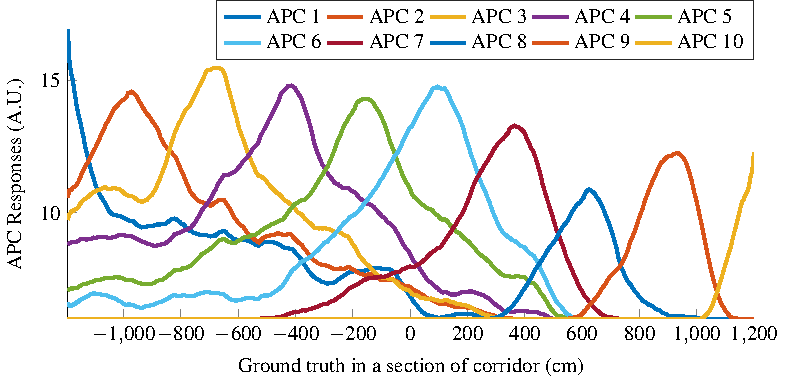
\includegraphics[width=4in]{gfx/Chapter05/APCRealResponses.pdf}
\caption{Responses from APCs.  The APCs are defined every 4 $m$ within a corridor, using ground truth information described in the experimental section.  Once defined, these APCs provide two different methods of localization.}
\label{fig:APCMany}
\end{figure}

The responses of the collection of APCs provide important information as a population code \cite{pouget2000information}.  By changing the threshold level, the support region of the APCs can be altered, leading to greater or lesser degrees of overlap, and (see Section \ref{sec:experiments}), different performance.


%
%\subsection{Multiple APCs}
%
%
%\label{sec:APC}
%Given the population code for a video sequence, represented by the tensor $\tens{S}_p$, we now aim to model the behaviour of place-cells themselves.   Population codes for individual frames are represented by the occurrences with which certain patterns in modes $i_3,i_4$ are observed within a frame.   Once encoded using the dictionary $\mathcal{V}$, which contains terms $t_1,t_2,...,t_{\mathcal{V}}$, the dimensions corresponding to the joint orientation and spatial encoding over patches is collapsed to a single term for each patch, and the set of numbers over the entire frame (dimensions $i_1,i_2$) are converted into a term-frequency representation \cite{Wu:2008} (see Fig.~\ref{fig:HistEncodings}).
%
%\begin{figure}
%\centering
%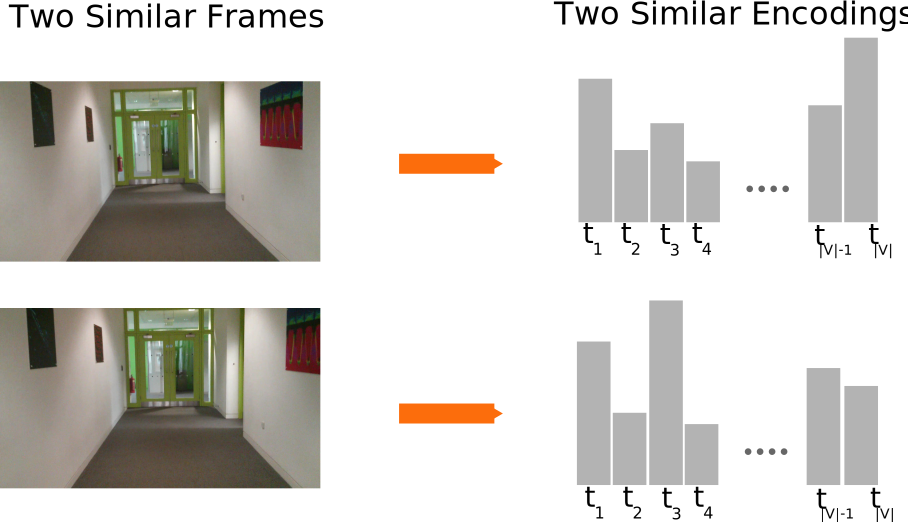
\includegraphics[width=3.5in]{gfx/Chapter05/HistogramEncodings.pdf}
%\caption{Two image frames should have similar representations along the fibre in the order 2 tensor that contains an encoded image sequence.  Here, two similar frames are shown with (diagrammatic) representations taken from along the fibre corresponding to particular frames.  The elements of the fibre correspond to dictionary terms, and the occurrence of each term is recorded.  We used the $\chi^2$ similarity measure.}
%\label{fig:HistEncodings}
%\end{figure}
%
%
%We found that the $\chi^2$ similarity measure was an appropriate way to compare two histograms. That is, individual fibres, one a single order 1 tensor $\mathbf{q}$ and a second drawn from a previously encoded sequence from a different journey, $\tens{S}_p$, yielded behaviour that decayed gently from the true location of the query shot when using the $\chi^2$ similarity measure, provided that very low similarity scores were thresholded out.  That is, due to the presence of noise, there is a threshold to the $\chi^2$ score above which place-cell like behaviour could be observed.  By varying the height at which APCs are considered to be active, the width of an APC response can be altered.  Altering APCs width is key to to methods of localization that are discussed in the next section.  



\subsection{Location from APC Activations}
Conceptually, given a series of APC responses to visual cues of a person's location along some journey -- illustrated in Fig.~\ref{fig:APC} -- there are two obvious ways of estimating location, $\ell$.  The first is simply to use the APC which displays maximum activation (firing rate) as a rough indicator of where the person is. That is, given a set of activations $p(r_i|\ell)$, the location of the camera that captured a particular image frame is provided by the index, $i$ associated with maximizing $p(r_i|\ell)$. This provides a precision that is limited by the width the APCs, but requires little more than ensuring that place cell responses are reasonably well-separated. 

The second technique to infer location achieves more accurate localisation of a camera from its captured visual data by using the joint distribution $p(\mathbf{r}|\ell)$, of APC responses, $\mathbf{r}$ to infer location $\ell$ relative to some designated ground truth.  We use a single index, $i$, to refer to the response of a unique place cell, $r_i$.

 First, a rough location may be identified by using \texttt{arg max}($r_i$) over the index, $i$; then, the responses of neighbouring APCs can be used to obtain sub-cell localisation.  In order to apply this principle, one needs sufficiently accurate estimates of $p(\mathbf{r}|\ell) = p(r_1,r_2,r_3,...,r_C|\ell)$, where $r_C$ is the total number of place cells in some region of a path.   Given several active cells that are a subset of all place cells in a location, sub-APC localisation is possible using APC responses from previous journeys using empirical Bayes' techniques. For example, if three cells are active, the chain rule can be used to obtain successively refined estimates of $\ell$:
\begin{eqnarray}
p(\ell|\mathbf{r}) & \propto & p(r_3,r_4,r_5|\ell)p(\ell) \nonumber \\
&\propto& p(r_3|r_4,r_5,\ell)\times p(r_4|r_5,\ell)\times p(r_5|\ell)\times p(\ell)
\end{eqnarray}
 so that the responses of spatially close APCs can be used to infer sub-APC position.  If the width of an APC is set to around 2 m, localisation of the order of tens of centimetres is plausible. 


%\subsubsection{BOVW model spatial binning as a form of population encoding}

%Here we need to include the notions of the spatial binning achieved during clustering as a form of population encoding: close locations in space correspond to close positions in V1 receptive fields. Expand.



\subsection{Overview of the System}
\label{ch05:overview}
In the experimental work to be discussed in the next section, a Generalized Regression Neural Network was used to provide sub-APC position estimates, obviating the need to construct {\em ad-hoc} empirical estimators.  This regression network consists of two-layers, and uses radial-basis functions.  The responses from $C = 16$ place cells were input to the network, and ground truth of location within a section of corridor -- up to 4 m long -- used to train it as a regressor.  In all experiments, dictionary generation was performed independently of the APC responses used in training the regression network. 

An overview of the pipeline for processing the frames to generate APCs is shown in Fig.~\ref{fig:pipeline}. The performance of different methods will be discussed in Section~\ref{sec:experiments}.


%\subsection{System Pipeline}

\begin{figure}[h]
\centering
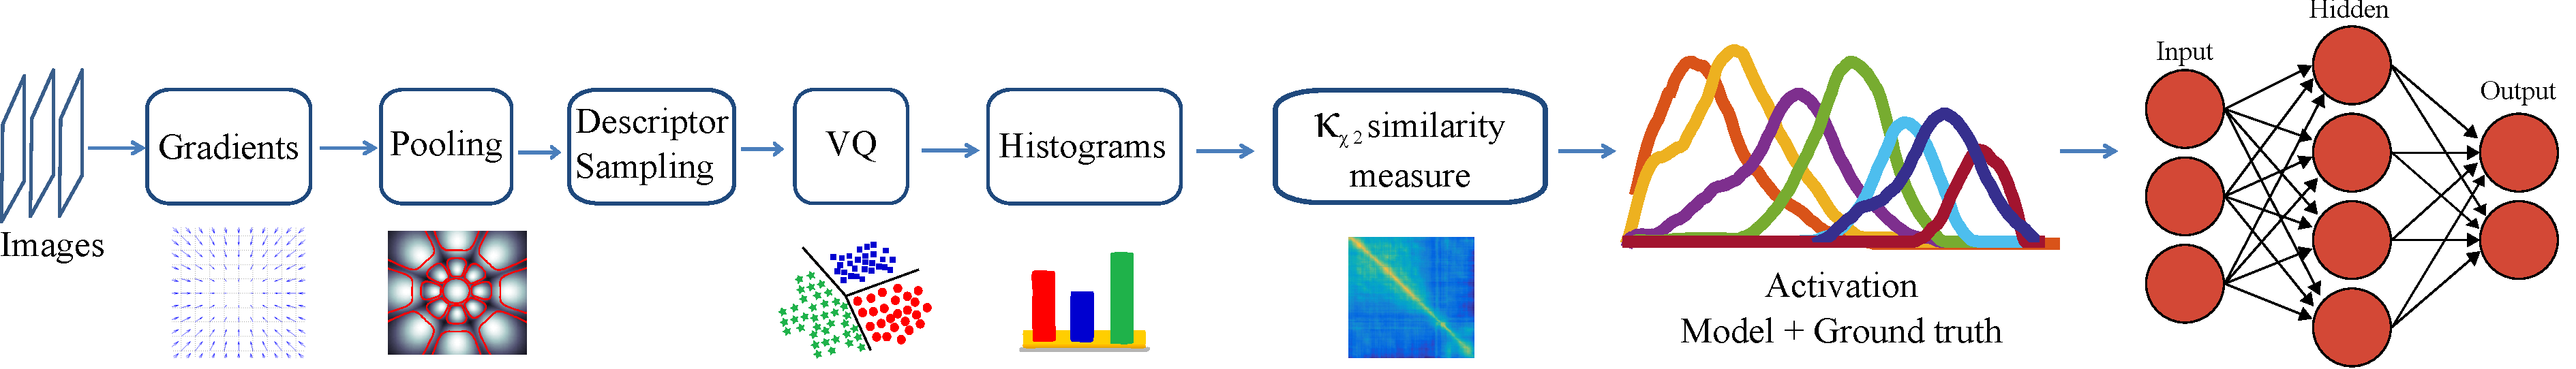
\includegraphics[width=\linewidth]{gfx/Chapter05/nn_pipeline.pdf}
\caption{Overview of the training pipeline. The diagram of the neural network is merely illustrative, it does not represent the real architecture used.}
\label{fig:pipeline}
\end{figure}

%\section{Decoding location representations: a neural network approach}



\section{Experiments and Results}
\label{sec:ch5experiments}

In order to test the APC concept, we performed a series of experiments using the publicly available RSM dataset~\cite{RiveraWearable}. We recall from Chapter \ref{ch:chapter4} that this dataset contains visual data of more than 3 km of indoor journeys acquired with two devices: a hand-held Nexus 4 and a wearable Google Glass. Corridors varied in length between 32 m and 60 m and the sequences comprise more than 120,000 frames with ground truth acquired with surveying equipment. The original resolution of the dataset is $1280 \times 720$ pixels per frame which we down-sampled to $208 \times 117$. 


%within one building of the Royal School of Mines at Imperial College.  Using a surveyor's wheel, we mapped out a number of one-dimensional corridors, measuring distance travelled and location within a corridor whilst simultaneously recording video-sequences from either a hand-held or a wearable camera. The surveyors wheel was modified to connect it directly to a data acquisition system (Raspberry Pi), which was synchronized to network time. Different human subjects held or wore the equipment, and walked at different rates along the corridors selected for the experiment. The video sequences were captured at between 25 to 30 frames per second at a resolution of $1280 \times 720$ pixels per frame, and were down-sampled to a pixel size of $208 \times 117$ per frame.  In total, over 100,000 frames of data were collected, corresponding to over $3 km$ of journey information.  Corridors varied in length between 32 m and 60 m.

%Using the network architecture, dictionary encoding and APC models described in earlier sections, the APC responses are generated from real data sequences.

%\subsection{APC modelling experiments}

%In Fig.~\ref{fig:APCSingleNoisy}, we show place cell responses from a single location, captured with multiple journeys.  The variability of responses is significant, but not unlike the types of variation found in biological variability, where multiple trials are usually required, together with averaging, in order to tease out average firing rate curves.

%\begin{figure}
%	\centering
%%	\setlength\figureheight{0.3\textwidth}
%%	\setlength\figurewidth{0.4\textwidth}
%%		% This file was created by matlab2tikz.
% Minimal pgfplots version: 1.3
%
%The latest updates can be retrieved from
%  http://www.mathworks.com/matlabcentral/fileexchange/22022-matlab2tikz
%where you can also make suggestions and rate matlab2tikz.
%
\definecolor{mycolor1}{rgb}{0.00000,0.44700,0.74100}%
\definecolor{mycolor2}{rgb}{0.85000,0.32500,0.09800}%

%
\begin{tikzpicture}

\begin{axis}[%
width=0.95092\figurewidth,
height=\figureheight,
at={(0\figurewidth,0\figureheight)},
scale only axis,
xmin=517,
xmax=816,
xlabel={Frame index},
ymin=1.79650837845272,
ymax=7.47640317281087,
ylabel={$\chi{}^\text{2}\text{ score}$}
]
\addplot [color=mycolor2,solid,line width=2.0pt,forget plot]
  table[row sep=crcr]{%
517	5.45564129617479\\
518	5.28480574819777\\
519	5.38022258546617\\
520	5.04640165964762\\
521	4.91818147235447\\
522	5.02140005429586\\
523	4.9060054090288\\
524	5.14407377772861\\
525	4.78613996505737\\
526	4.74626959694756\\
527	4.60538254843818\\
528	4.73193724950155\\
529	4.89160471492344\\
530	4.61402278476291\\
531	4.74068803257412\\
532	4.82834929890103\\
533	4.78515206442939\\
534	5.00995551215278\\
535	4.93059447076586\\
536	4.747631099489\\
537	4.85051237212287\\
538	4.85323116514418\\
539	4.79317005475362\\
540	4.78844994968838\\
541	4.7296888033549\\
542	4.57528159353468\\
543	4.6541080739763\\
544	4.73621863789029\\
545	4.60128768285116\\
546	4.72721687952677\\
547	4.7022082540724\\
548	4.51559209823608\\
549	4.45021396213108\\
550	4.61597768465678\\
551	4.58577950795492\\
552	4.56056160397\\
553	4.61316866344876\\
554	4.44940259721544\\
555	4.33124679989285\\
556	4.31974034839206\\
557	4.24667429924011\\
558	4.18328481250339\\
559	4.32105019357469\\
560	4.36144169171651\\
561	4.33154243893093\\
562	4.2965227233039\\
563	4.45881326993306\\
564	4.60404780175951\\
565	4.9832649230957\\
566	5.21849367353651\\
567	5.42206896675958\\
568	5.61464606391059\\
569	5.32002242406209\\
570	5.31870725419786\\
571	5.20021793577406\\
572	5.55876763661702\\
573	5.52424425548977\\
574	5.40127817789714\\
575	5.50023322635227\\
576	5.73416566848755\\
577	5.55387417475383\\
578	5.5627646446228\\
579	5.47471041149563\\
580	5.35248724619548\\
581	4.86793337927924\\
582	4.91971654362149\\
583	4.92856052186754\\
584	5.1939090622796\\
585	4.77915970484416\\
586	4.61318797535366\\
587	4.59124125374688\\
588	4.83357630835639\\
589	4.78117969301012\\
590	4.8751319249471\\
591	5.01082160737779\\
592	5.23354652192858\\
593	4.6385703086853\\
594	4.53041002485487\\
595	4.51224210527208\\
596	4.43363348642985\\
597	4.25946267445882\\
598	4.22609305381775\\
599	4.34774973657396\\
600	4.57303765085008\\
601	4.32682673136393\\
602	4.77783237563239\\
603	4.9052480061849\\
604	4.89262798097399\\
605	4.71505321396722\\
606	4.99992277887132\\
607	4.91769223743015\\
608	4.94722530576918\\
609	5.03998618655735\\
610	4.98740741941664\\
611	5.11870463689168\\
612	5.16300662358602\\
613	5.19595686594645\\
614	5.05345845222473\\
615	4.81346085336473\\
616	4.98365359836155\\
617	5.10461118486193\\
618	5.3875585132175\\
619	5.45500458611382\\
620	5.10809373855591\\
621	5.40080017513699\\
622	5.12411006291707\\
623	5.11253976821899\\
624	5.29478883743286\\
625	5.38006231519911\\
626	5.26761012607151\\
627	5.07983054055108\\
628	4.79844037691752\\
629	4.7360757721795\\
630	4.55040812492371\\
631	4.55683490965101\\
632	4.32798796229892\\
633	4.38316342565748\\
634	4.57085434595744\\
635	4.71197700500488\\
636	5.20676475101047\\
637	5.29618379804823\\
638	5.53390868504842\\
639	5.37041934331258\\
640	5.56473557154338\\
641	5.70307895872328\\
642	5.30179659525553\\
643	5.38066954082913\\
644	5.54609791437785\\
645	5.42192618052165\\
646	5.84239138497247\\
647	5.49786647160848\\
648	5.54475773705377\\
649	5.51714981926812\\
650	5.45711406071981\\
651	5.44256104363336\\
652	5.12285571628147\\
653	5.11807007259793\\
654	5.33797539605035\\
655	5.66756502787272\\
656	5.50892194112142\\
657	5.86675696902805\\
658	5.8700491587321\\
659	5.71904346677992\\
660	5.90887721379598\\
661	6.13676097657945\\
662	6.19742769665188\\
663	6.42192517386542\\
664	6.30267741945055\\
665	6.34279457728068\\
666	6.27500221464369\\
667	6.28113868501451\\
668	6.38645627763536\\
669	6.43902895185682\\
670	6.78609715567695\\
671	6.9065891901652\\
672	6.71403990851508\\
673	6.70098299450344\\
674	6.66558986239963\\
675	6.7139032681783\\
676	6.78372716903687\\
677	6.76429753833347\\
678	7.00557661056519\\
679	6.82014653417799\\
680	7.00547329584758\\
681	7.34336815940009\\
682	7.20823060141669\\
683	6.99682813220554\\
684	7.24651824103461\\
685	7.23865800433689\\
686	7.34053574668037\\
687	7.34751473532783\\
688	7.37640317281087\\
689	7.37493318981594\\
690	7.32039319144355\\
691	7.26464568244086\\
692	7.08425818549262\\
693	6.96295788553026\\
694	6.90606005986532\\
695	7.08241897159153\\
696	6.66772707303365\\
697	6.62142117818197\\
698	6.64435042275323\\
699	6.69112764464484\\
700	6.59604427549574\\
701	6.51153024037679\\
702	6.47479195064968\\
703	6.78648434744941\\
704	6.22314156426324\\
705	5.96851372718811\\
706	6.07606569925944\\
707	6.0125810570187\\
708	6.13718112309774\\
709	6.05301419893901\\
710	5.86252167489794\\
711	5.8945533964369\\
712	5.94143915176392\\
713	5.79714462492201\\
714	5.77606577343411\\
715	5.80971254242791\\
716	5.595112880071\\
717	5.6970772213406\\
718	5.93423128128052\\
719	5.84677373038398\\
720	5.82072750727336\\
721	5.70003567801581\\
722	5.5985779232449\\
723	5.41437101364136\\
724	5.41969439718458\\
725	5.26762652397156\\
726	5.31281068589952\\
727	5.33975100517273\\
728	5.22491206063165\\
729	5.03604883617825\\
730	5.22387671470642\\
731	5.00555160310533\\
732	4.94978168275621\\
733	4.51597449514601\\
734	4.7652227083842\\
735	4.92013684908549\\
736	4.85085704591539\\
737	4.84549196561178\\
738	4.6559042930603\\
739	4.86927668253581\\
740	4.71941457854377\\
741	4.81414641274346\\
742	4.79970055156284\\
743	4.69480657577515\\
744	4.71684855884976\\
745	4.59916199578179\\
746	4.60451703601413\\
747	4.55340411927965\\
748	4.76788369814555\\
749	4.70615172386169\\
750	4.6492067972819\\
751	4.7372952832116\\
752	4.70831603474087\\
753	4.95494400130378\\
754	4.93097477489048\\
755	5.05009076330397\\
756	4.83696320321825\\
757	4.65081408288744\\
758	4.9603201813168\\
759	5.27593053711785\\
760	5.34850931167603\\
761	5.34796449873182\\
762	5.31409517923991\\
763	5.15496057934231\\
764	5.20180945926242\\
765	5.18936035368178\\
766	4.8254066573249\\
767	5.08930932150947\\
768	4.86718906296624\\
769	4.62061770757039\\
770	4.98884542783101\\
771	5.15281282530891\\
772	5.03079618348016\\
773	4.79297688272264\\
774	4.88556533389621\\
775	5.0670190387302\\
776	4.6277256541782\\
777	4.46976200739543\\
778	4.50152950816684\\
779	4.35459629694621\\
780	4.15776922967699\\
781	4.18754514058431\\
782	4.16014623641968\\
783	4.23905968666077\\
784	4.11976922882928\\
785	3.84921227561103\\
786	4.09121913380093\\
787	4.26308623949687\\
788	3.93736775716146\\
789	4.12939588228862\\
790	4.14773575464884\\
791	4.02434510654873\\
792	3.93602151340908\\
793	3.89979214138455\\
794	3.81887470351325\\
795	3.75678775045607\\
796	3.81119052569071\\
797	3.97538926866319\\
798	3.73644529448615\\
799	3.62051859166887\\
800	3.63900767432319\\
801	3.4945670498742\\
802	3.44758110576206\\
803	3.41365891032749\\
804	3.53506263097127\\
805	3.68221312099033\\
806	3.50561817487081\\
807	3.18562004301283\\
808	2.92959801355998\\
809	2.77806928422716\\
810	2.53599411911435\\
811	2.5533709526062\\
812	2.44258156087663\\
813	2.23334169387817\\
814	1.9372197786967\\
815	1.97369148996141\\
816	1.79650837845272\\
};


\addplot [color=mycolor1,solid,line width=2.0pt,forget plot]
  table[row sep=crcr]{%
517	5.45564129617479\\
518	5.37355654327958\\
519	5.21705055236816\\
520	5.14466546073792\\
521	5.10476355199461\\
522	5.02677491939429\\
523	4.99369739059709\\
524	4.95151845967328\\
525	4.93448695637821\\
526	4.9382541179657\\
527	4.9249986529981\\
528	4.91614664925469\\
529	4.90358046743605\\
530	4.88218153160786\\
531	4.86746233359151\\
532	4.85760750992751\\
533	4.83489814751879\\
534	4.82152560173519\\
535	4.80884125211217\\
536	4.78737886475022\\
537	4.76278513104612\\
538	4.73903547392951\\
539	4.7215891002137\\
540	4.70695415963518\\
541	4.71049302505528\\
542	4.7056532776545\\
543	4.70845456782923\\
544	4.71323872045054\\
545	4.71882281768349\\
546	4.72699681323131\\
547	4.73064615775128\\
548	4.74396783586532\\
549	4.75172641704412\\
550	4.76428025812248\\
551	4.77966727096748\\
552	4.80270366117257\\
553	4.8194778841369\\
554	4.83317502555933\\
555	4.85074007916613\\
556	4.8632257774033\\
557	4.86403361577836\\
558	4.86677982963942\\
559	4.86511870738871\\
560	4.87049247456246\\
561	4.87113591548807\\
562	4.86629256045197\\
563	4.86094582756631\\
564	4.86177044498677\\
565	4.8616220724015\\
566	4.86459029937277\\
567	4.87347887108385\\
568	4.88530414553186\\
569	4.88331132248686\\
570	4.88186483967061\\
571	4.8774775993797\\
572	4.87199648167271\\
573	4.86676935057521\\
574	4.86219545448719\\
575	4.85672141473039\\
576	4.85646137683029\\
577	4.85169127738935\\
578	4.85505176131147\\
579	4.86435472884146\\
580	4.87581148763903\\
581	4.88387909714056\\
582	4.89925151509222\\
583	4.91423942172338\\
584	4.92701850564572\\
585	4.9408663524792\\
586	4.95425135208095\\
587	4.97103057480723\\
588	4.98540186773893\\
589	4.99748164455907\\
590	4.9989141655617\\
591	4.99064818963983\\
592	4.98170093722354\\
593	4.97129206214092\\
594	4.9726703496747\\
595	4.97545192787707\\
596	4.97357184221955\\
597	4.97034801647506\\
598	4.96218201254501\\
599	4.95628939193933\\
600	4.95209664930832\\
601	4.94487005026162\\
602	4.93902792681912\\
603	4.92917212877684\\
604	4.91537069949974\\
605	4.90279087349941\\
606	4.89631076626767\\
607	4.88890501863562\\
608	4.87664843578728\\
609	4.86010260646846\\
610	4.85585147669526\\
611	4.85786757934121\\
612	4.87042928336699\\
613	4.87987025254438\\
614	4.89523206870842\\
615	4.90533997520568\\
616	4.9166443418213\\
617	4.92622663644977\\
618	4.93976186678793\\
619	4.95711410180782\\
620	4.97821319995283\\
621	4.99838243860777\\
622	5.03068710616927\\
623	5.05664166571602\\
624	5.08107040041969\\
625	5.10033799569353\\
626	5.12340508404773\\
627	5.13697097523142\\
628	5.14141194890686\\
629	5.14601280791959\\
630	5.15872550551313\\
631	5.17235085753356\\
632	5.1844167698538\\
633	5.2031827221652\\
634	5.22012278282183\\
635	5.2350541307272\\
636	5.25118010168443\\
637	5.27105263950062\\
638	5.2914908197191\\
639	5.31941871199748\\
640	5.34981088681556\\
641	5.37754845781391\\
642	5.40143398903395\\
643	5.41967031907062\\
644	5.43867953726494\\
645	5.46584148039353\\
646	5.49411284734332\\
647	5.5304899723892\\
648	5.56317364872178\\
649	5.59187148866199\\
650	5.61810674472731\\
651	5.64762293130092\\
652	5.68239633188226\\
653	5.72251586578871\\
654	5.76883220942923\\
655	5.81515340145483\\
656	5.86512561341802\\
657	5.92666398478744\\
658	5.98431841694579\\
659	6.03382808605289\\
660	6.08555341740044\\
661	6.127020626652\\
662	6.16874209499143\\
663	6.20575446336448\\
664	6.24669290886444\\
665	6.28363571740062\\
666	6.31664213031328\\
667	6.35670027494971\\
668	6.39146739014693\\
669	6.42038289976228\\
670	6.4506713462795\\
671	6.4759780317207\\
672	6.49985273787224\\
673	6.52182546116057\\
674	6.54482955510925\\
675	6.57001350580159\\
676	6.59355397992123\\
677	6.62189427633134\\
678	6.64958247792424\\
679	6.67914388509565\\
680	6.69048218175668\\
681	6.69986160596212\\
682	6.70413321270153\\
683	6.70704202695228\\
684	6.71557544850979\\
685	6.71851701963516\\
686	6.71292029919268\\
687	6.70673919102502\\
688	6.69693335383928\\
689	6.68661635803257\\
690	6.67505046407652\\
691	6.66555475648028\\
692	6.65155422984878\\
693	6.63748526951623\\
694	6.62718327623916\\
695	6.60801341041686\\
696	6.58585296790886\\
697	6.56515900402112\\
698	6.54266094134238\\
699	6.51712586279629\\
700	6.49071343685764\\
701	6.45977260736652\\
702	6.4301504267046\\
703	6.39615398577822\\
704	6.36359818019564\\
705	6.32340584428403\\
706	6.2801509168413\\
707	6.2351982842227\\
708	6.19342182607067\\
709	6.13769644350151\\
710	6.08721817215554\\
711	6.03782227628626\\
712	5.98687007854315\\
713	5.93521882941664\\
714	5.87972844376856\\
715	5.82970565787248\\
716	5.77776216595622\\
717	5.73143335426746\\
718	5.68728524541098\\
719	5.64215762328669\\
720	5.59388067608788\\
721	5.55166506226641\\
722	5.51050375324258\\
723	5.4678313797023\\
724	5.42858150324313\\
725	5.3900122674955\\
726	5.35200566661601\\
727	5.31654655095401\\
728	5.27413495273547\\
729	5.24825336981793\\
730	5.22707910548532\\
731	5.20614084148623\\
732	5.18214864038826\\
733	5.15181461915948\\
734	5.12951474124882\\
735	5.11754349353903\\
736	5.10639973670717\\
737	5.09428800909427\\
738	5.08442985714158\\
739	5.07175424093562\\
740	5.0593480555649\\
741	5.05106739176103\\
742	5.03327819657704\\
743	5.01603489127559\\
744	4.99604336745074\\
745	4.97155133072211\\
746	4.95703724398364\\
747	4.94793999708699\\
748	4.9401119393286\\
749	4.92732178597223\\
750	4.91952461882784\\
751	4.91450846276316\\
752	4.89997733315102\\
753	4.88456610757477\\
754	4.87365754986025\\
755	4.85591713317127\\
756	4.8386154520809\\
757	4.82305960428147\\
758	4.81579780308297\\
759	4.80505978223148\\
760	4.78872574916502\\
761	4.76828401915881\\
762	4.75289069606063\\
763	4.74487400108995\\
764	4.72585545159251\\
765	4.71381425370975\\
766	4.70021403619762\\
767	4.68439045568713\\
768	4.66890504625108\\
769	4.65223042548649\\
770	4.63630619503203\\
771	4.61900559736758\\
772	4.60385838117189\\
773	4.58768502546816\\
774	4.56789509833805\\
775	4.54690146148881\\
776	4.52448742865435\\
777	4.49971704120809\\
778	4.46895453313581\\
779	4.43798890324677\\
780	4.40706996177059\\
781	4.38350363356186\\
782	4.36013228850029\\
783	4.32391391833083\\
784	4.27602958111536\\
785	4.22357162137151\\
786	4.16618447076707\\
787	4.10984316001944\\
788	4.0544884861732\\
789	3.99390751136944\\
790	3.92753729555342\\
791	3.86933902683171\\
792	3.80213900758566\\
793	3.76206392768427\\
794	3.70389658551157\\
795	3.64771100655391\\
796	3.58290216851687\\
797	3.533371826862\\
798	3.48501014709473\\
799	3.44571603063553\\
800	3.400025913611\\
801	3.36231850466848\\
802	3.30612304384224\\
803	3.25225202340648\\
804	3.1855489508311\\
805	3.12186565721668\\
806	3.05844036485783\\
807	2.97056146671897\\
808	2.88727670479444\\
809	2.79667528382054\\
810	2.69914532624758\\
811	2.53378304447791\\
812	2.35337503015259\\
813	2.21038685336946\\
814	2.07666858037313\\
815	1.90247321570361\\
816	1.79650837845272\\
};

\end{axis}
\end{tikzpicture}%

%	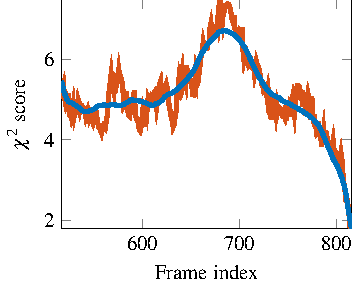
\includegraphics[width=.4\textwidth, height=.3\textwidth]{gfx/Chapter05/single_tuning_curve.pdf}
%	\caption{Single APC tuning curve (raw measurements in red) and a smoothed
%version (blue trace). The APC response must be thresholded before using it
%for accurate position inference; super-threshold responses from a number of
%APCs at different positions in the same corridor are shown in Fig. ~\ref{fig:multipleAPCs}.}
%\label{fig:APCSingleNoisy}
%\end{figure}

%In Fig.~\ref{fig:APCMany}, the average responses from each of several APC cell responses is plotted along a length of corridor in one corridor.  These curves are produced by setting place cell locations to be spaced every 4 m within a single corridor, and constructing the average APC responses using the $\kappa_{\chi^2}$ distance metric between dictionary-encoded population codes.



\subsection{APC-level Localization}
\label{subsec:inferloc}

The first method used to infer location -- based on identifying the APC with maximum activity -- was tested in several corridors of the experimental data.  First, a visualization showing the locations of APCs with maximum activation is shown in Fig.~\ref{fig:floorplan}; these are indicated on the floor plan of one of the building sections that was used to conduct the experiment.  Locations are staggered across the width of the corridor in order to visualize the individual activations of the 8 APCs defined within this corridor. The second technique to estimate location relies on the overlap of the responses from APCs and the use of a GRNN. Table \ref{table:methodComparison} compares the two localisation techniques for different methods of descriptor generation. A dictionary based on a single device type was used, but all the combinations of remaining passes were submitted as queries. The neural network regressor shows better results, achieving errors as low as 2.49 m for SF-GABOR, even with the majority of the queries coming from a different device that was not used to learn the dictionary. Very low errors were observed using a single device, as may be seen in Fig.~\ref{fig:sublocMethodComp}. The performance of LSD-SLAM, when tested on the same sequences, is also reported, but tracking was lost in roughly 40\% of sequences. This is probably because LSD-SLAM performs best on sequences acquired with global-shutter, fish-eye lenses. The RSM dataset does not use such cameras. A tracking recovery exception catch was therefore implemented to keep LSD-SLAM running. 




%\begin{figure}
%\begin{center}
%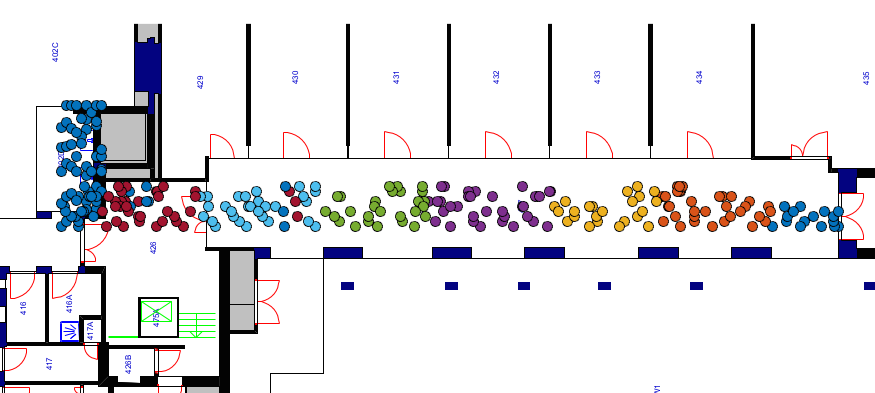
\includegraphics[width=.8\linewidth]{gfx/Chapter05/placeCellsExperiment_withDetection_5px_horiz.png}
%\caption{Using ground truth from a surveyor's wheel, activations from APCs are overlaid onto the floor plan in which video data was acquired. Different colours refer to individual APCs, and activations are staggered across the width of the corridor to allow visualization.}
%\label{fig:floorplan}
%\end{center}
%\end{figure}



\subsection{Sub-APC Localization}


By arranging for APC responses to be up to 4 m in width, the responses from several cells can be used to perform accurate inference of spatial position using a single section of corridor.  The success of this technique is illustrated in Fig.~\ref{fig:sublocMethodComp}. Note that average absolute errors are very small compared to distances traversed.


\begin{figure}
\centering
	\setlength\figureheight{0.6\linewidth}
	\setlength\figurewidth{0.8\linewidth}
		% This file was created by matlab2tikz.
% Minimal pgfplots version: 1.3
%
%The latest updates can be retrieved from
%  http://www.mathworks.com/matlabcentral/fileexchange/22022-matlab2tikz
%where you can also make suggestions and rate matlab2tikz.
%
\definecolor{mycolor1}{rgb}{0.00000,0.44700,0.74100}%
\definecolor{mycolor2}{rgb}{0.85000,0.32500,0.09800}%
\definecolor{mycolor3}{rgb}{0.00000,0.44706,0.74118}%
\definecolor{mycolor4}{rgb}{0.85098,0.32549,0.09804}%
\definecolor{mycolor5}{rgb}{0.00000,0.49804,0.00000}%
\definecolor{mycolor6}{rgb}{0.00000,0.74902,0.74902}%
\definecolor{mycolor7}{rgb}{0.92941,0.69412,0.12549}%
%
\begin{tikzpicture}

\begin{axis}[%
width=0.410625\figurewidth,
height=0.418605\figureheight,
at={(0\figurewidth,0.581395\figureheight)},
scale only axis,
xmin=0,
xmax=100,
xlabel={Query frame index},
ymin=0,
ymax=30,
ylabel={Position (m)},
legend style={at={(0.01,0.98)},anchor=north west,legend cell align=left,align=left,draw=white!15!black}
]
\addplot [color=mycolor1,mark size=2.5pt,only marks,mark=*,mark options={solid}]
  table[row sep=crcr]{%
1	3.82933075138807\\
2	4.13785727959975\\
3	4.0447361707515\\
4	4.2529130246433\\
5	4.20690402917172\\
6	4.50063950188439\\
7	4.75352080933664\\
8	4.74326159397881\\
9	4.91108240960902\\
10	5.12462525162416\\
11	5.38575790168879\\
12	5.5983549587032\\
13	5.88469331410338\\
14	6.37724895389065\\
15	6.49707000927523\\
16	6.97599308950192\\
17	7.0084637125246\\
18	7.25574078865362\\
19	7.68246217820926\\
20	7.47868037243643\\
21	8.3361547709122\\
22	8.13515172855731\\
23	8.71807646819173\\
24	8.74624527757843\\
25	9.24807476954356\\
26	9.39137711769411\\
27	9.47111462832638\\
28	9.62707845342908\\
29	9.8688285534354\\
30	10.1001373757242\\
31	10.1523303389699\\
32	10.303533206715\\
33	10.7146855366354\\
34	10.8227845020693\\
35	11.3176424734392\\
36	11.4926054393774\\
37	11.9903703427759\\
38	12.2721100872506\\
39	12.3176264271314\\
40	12.515011373852\\
41	13.1766609753065\\
42	12.9990856928756\\
43	13.1280085352542\\
44	13.6372082927005\\
45	13.7908178524479\\
46	14.1830357248297\\
47	14.3440978171742\\
48	14.4118815790833\\
49	14.7773588854047\\
50	15.3101475432747\\
51	15.3335835204922\\
52	15.3943311538839\\
53	15.6036565996397\\
54	15.9825309811509\\
55	16.1524192024403\\
56	16.6173626985367\\
57	16.7636132233496\\
58	16.9467149648138\\
59	17.0613097876886\\
60	17.3362003519623\\
61	17.3788095851072\\
62	17.7863337933338\\
63	17.938152225062\\
64	18.1826860945178\\
65	18.3522659094664\\
66	18.666467070377\\
67	19.2033718195273\\
68	19.2732842904444\\
69	19.4961336317471\\
70	19.7047748119942\\
71	20.0018674335363\\
72	20.1693726438626\\
73	20.646451485791\\
74	20.6623474464074\\
75	20.686437609905\\
76	20.9364803251298\\
77	21.4051420449512\\
78	21.7297401569254\\
79	21.7725537505229\\
80	21.9992940185493\\
81	22.1414204593795\\
82	22.5556984563659\\
83	22.651679993547\\
84	22.8472028540663\\
85	23.2393311221328\\
86	23.8784854455955\\
87	24.8139340298392\\
88	24.2471293259343\\
89	24.416470388524\\
90	25.1233083160561\\
91	24.9044698130965\\
92	24.9779646677297\\
93	25.1144252216639\\
94	25.5752279222371\\
95	25.916221928035\\
96	26.1095563745674\\
97	26.3265866080742\\
98	26.5073258582685\\
99	26.6868609530868\\
100	26.8356908497233\\
};
\addlegendentry{\footnotesize{DSIFT estimate}};

\addplot [color=mycolor2,mark size=1pt,only marks,mark=*,mark options={solid}]
  table[row sep=crcr]{%
1	3.34279475982533\\
2	3.58455648184906\\
3	3.82631820387279\\
4	4.06807992589652\\
5	4.30984164792025\\
6	4.55160336994398\\
7	4.79336509196771\\
8	5.03512681399144\\
9	5.27688853601517\\
10	5.5186502580389\\
11	5.76041198006263\\
12	6.00217370208637\\
13	6.2439354241101\\
14	6.48569714613383\\
15	6.72745886815756\\
16	6.96922059018129\\
17	7.21098231220502\\
18	7.45274403422875\\
19	7.69450575625248\\
20	7.93626747827621\\
21	8.17802920029994\\
22	8.41979092232367\\
23	8.6615526443474\\
24	8.90331436637113\\
25	9.14507608839486\\
26	9.3868378104186\\
27	9.62859953244233\\
28	9.87036125446606\\
29	10.1121229764898\\
30	10.3538846985135\\
31	10.5956464205372\\
32	10.837408142561\\
33	11.0791698645847\\
34	11.3209315866084\\
35	11.5626933086322\\
36	11.8044550306559\\
37	12.0462167526796\\
38	12.2879784747034\\
39	12.5297401967271\\
40	12.7715019187508\\
41	13.0132636407746\\
42	13.2550253627983\\
43	13.496787084822\\
44	13.7385488068457\\
45	13.9803105288695\\
46	14.2220722508932\\
47	14.4638339729169\\
48	14.7055956949407\\
49	14.9473574169644\\
50	15.1891191389881\\
51	15.4308808610119\\
52	15.6726425830356\\
53	15.9144043050593\\
54	16.1561660270831\\
55	16.3979277491068\\
56	16.6396894711305\\
57	16.8814511931542\\
58	17.123212915178\\
59	17.3649746372017\\
60	17.6067363592254\\
61	17.8484980812492\\
62	18.0902598032729\\
63	18.3320215252966\\
64	18.5737832473204\\
65	18.8155449693441\\
66	19.0573066913678\\
67	19.2990684133916\\
68	19.5408301354153\\
69	19.782591857439\\
70	20.0243535794627\\
71	20.2661153014865\\
72	20.5078770235102\\
73	20.7496387455339\\
74	20.9914004675577\\
75	21.2331621895814\\
76	21.4749239116051\\
77	21.7166856336289\\
78	21.9584473556526\\
79	22.2002090776763\\
80	22.4419707997001\\
81	22.6837325217238\\
82	22.9254942437475\\
83	23.1672559657712\\
84	23.409017687795\\
85	23.6507794098187\\
86	23.8925411318424\\
87	24.1343028538662\\
88	24.3760645758899\\
89	24.6178262979136\\
90	24.8595880199374\\
91	25.1013497419611\\
92	25.3431114639848\\
93	25.5848731860086\\
94	25.8266349080323\\
95	26.068396630056\\
96	26.3101583520797\\
97	26.5519200741035\\
98	26.7936817961272\\
99	27.0354435181509\\
100	27.2772052401747\\
};
\addlegendentry{\footnotesize{Ground Truth}};

\addplot [color=mycolor3,mark size=2.5pt,only marks,mark=*,mark options={solid},forget plot]
  table[row sep=crcr]{%
1	3.96138624563951\\
2	4.02384144631341\\
3	4.08707644791465\\
4	4.18828446195071\\
5	4.26415858284719\\
6	4.75415487269568\\
7	4.6964821475799\\
8	4.75798931619968\\
9	5.07543654699405\\
10	5.10422065555799\\
11	5.45794029015593\\
12	5.76040368536791\\
13	5.80472114525924\\
14	6.13479685019936\\
15	6.46654565238381\\
16	7.12191369259817\\
17	7.27995604403394\\
18	7.15523188589885\\
19	7.35322247628246\\
20	7.88688617297149\\
21	8.26681390322706\\
22	8.44517996598085\\
23	8.72260771329284\\
24	8.84429240760012\\
25	9.23564026303767\\
26	9.43208080980961\\
27	9.65282394064002\\
28	9.85363684446219\\
29	9.99229696790916\\
30	9.82724704176612\\
31	10.1565686496934\\
32	10.4590372105691\\
33	10.9156017837373\\
34	10.6291725658663\\
35	11.4705966920895\\
36	11.4892975051227\\
37	11.8408379725695\\
38	12.0921935140929\\
39	12.4349380865186\\
40	12.6553131611547\\
41	12.7772242694122\\
42	13.0523023918089\\
43	13.0256284815907\\
44	13.6524934330773\\
45	13.8238022889364\\
46	13.9609204475434\\
47	14.297286343374\\
48	14.4561293778333\\
49	14.8402142863425\\
50	15.5052024264221\\
51	15.5057419891046\\
52	15.6606840094501\\
53	15.9662200662868\\
54	16.0328546467595\\
55	16.2111955221519\\
56	16.6360512850595\\
57	16.7366179247953\\
58	16.8596816736172\\
59	17.0782243170383\\
60	17.1485506836758\\
61	17.3699216063894\\
62	17.9148139554418\\
63	18.2654521245055\\
64	18.3661786448842\\
65	18.4313081066571\\
66	18.8264914036045\\
67	19.1101534022013\\
68	19.0802132065578\\
69	19.335390004613\\
70	19.8370796974601\\
71	20.2097803608945\\
72	20.2433329080228\\
73	20.4599434575278\\
74	20.6607630368463\\
75	21.0132387710476\\
76	21.06208788754\\
77	21.4826688498949\\
78	21.5060719259411\\
79	21.6770129575088\\
80	21.9906413251447\\
81	22.1633629006305\\
82	22.6554650420082\\
83	22.8390757011666\\
84	23.0380700242874\\
85	23.1911470803173\\
86	23.8245634024496\\
87	24.8359027449437\\
88	24.2238149680853\\
89	24.3698839392998\\
90	24.8448344606137\\
91	24.6201567865696\\
92	24.9439712087726\\
93	25.2126775489935\\
94	25.5856674729661\\
95	25.9414437358967\\
96	26.1012903889201\\
97	26.3535315112959\\
98	26.5398191674684\\
99	26.7447081668017\\
100	26.8387537558918\\
};
\addplot [color=mycolor4,mark size=1.3pt,only marks,mark=*,mark options={solid},forget plot]
  table[row sep=crcr]{%
1	3.34279475982533\\
2	3.58455648184906\\
3	3.82631820387279\\
4	4.06807992589652\\
5	4.30984164792025\\
6	4.55160336994398\\
7	4.79336509196771\\
8	5.03512681399144\\
9	5.27688853601517\\
10	5.5186502580389\\
11	5.76041198006263\\
12	6.00217370208637\\
13	6.2439354241101\\
14	6.48569714613383\\
15	6.72745886815756\\
16	6.96922059018129\\
17	7.21098231220502\\
18	7.45274403422875\\
19	7.69450575625248\\
20	7.93626747827621\\
21	8.17802920029994\\
22	8.41979092232367\\
23	8.6615526443474\\
24	8.90331436637113\\
25	9.14507608839486\\
26	9.3868378104186\\
27	9.62859953244233\\
28	9.87036125446606\\
29	10.1121229764898\\
30	10.3538846985135\\
31	10.5956464205372\\
32	10.837408142561\\
33	11.0791698645847\\
34	11.3209315866084\\
35	11.5626933086322\\
36	11.8044550306559\\
37	12.0462167526796\\
38	12.2879784747034\\
39	12.5297401967271\\
40	12.7715019187508\\
41	13.0132636407746\\
42	13.2550253627983\\
43	13.496787084822\\
44	13.7385488068457\\
45	13.9803105288695\\
46	14.2220722508932\\
47	14.4638339729169\\
48	14.7055956949407\\
49	14.9473574169644\\
50	15.1891191389881\\
51	15.4308808610119\\
52	15.6726425830356\\
53	15.9144043050593\\
54	16.1561660270831\\
55	16.3979277491068\\
56	16.6396894711305\\
57	16.8814511931542\\
58	17.123212915178\\
59	17.3649746372017\\
60	17.6067363592254\\
61	17.8484980812492\\
62	18.0902598032729\\
63	18.3320215252966\\
64	18.5737832473204\\
65	18.8155449693441\\
66	19.0573066913678\\
67	19.2990684133916\\
68	19.5408301354153\\
69	19.782591857439\\
70	20.0243535794627\\
71	20.2661153014865\\
72	20.5078770235102\\
73	20.7496387455339\\
74	20.9914004675577\\
75	21.2331621895814\\
76	21.4749239116051\\
77	21.7166856336289\\
78	21.9584473556526\\
79	22.2002090776763\\
80	22.4419707997001\\
81	22.6837325217238\\
82	22.9254942437475\\
83	23.1672559657712\\
84	23.409017687795\\
85	23.6507794098187\\
86	23.8925411318424\\
87	24.1343028538662\\
88	24.3760645758899\\
89	24.6178262979136\\
90	24.8595880199374\\
91	25.1013497419611\\
92	25.3431114639848\\
93	25.5848731860086\\
94	25.8266349080323\\
95	26.068396630056\\
96	26.3101583520797\\
97	26.5519200741035\\
98	26.7936817961272\\
99	27.0354435181509\\
100	27.2772052401747\\
};
\end{axis}

\begin{axis}[%
width=0.410625\figurewidth,
height=0.418605\figureheight,
at={(0.540296\figurewidth,0.581395\figureheight)},
scale only axis,
xmin=0,
xmax=100,
xlabel={Query frame index},
ymin=0,
ymax=30,
ylabel={Position (m)},
legend style={at={(0.05,0.98)},anchor=north west,legend cell align=left,align=left,draw=white!15!black}
]
\addplot [color=mycolor5,mark size=2.5pt,only marks,mark=*,mark options={solid}]
  table[row sep=crcr]{%
1	3.93380316517375\\
2	4.02010797239491\\
3	4.07403562972169\\
4	4.22960858717326\\
5	4.49281191982221\\
6	4.48128404061484\\
7	4.71319196570184\\
8	4.86319964191374\\
9	5.09887668580362\\
10	5.21915019696987\\
11	5.63572784312706\\
12	5.74127734329797\\
13	5.87169080731423\\
14	6.31299989760469\\
15	6.60880852770678\\
16	7.17088323462264\\
17	7.14775319012465\\
18	7.12756218272848\\
19	7.44319950471791\\
20	7.91093596766044\\
21	8.2270189482985\\
22	8.53219031334255\\
23	8.61950521326314\\
24	8.79443298854439\\
25	9.16512641081381\\
26	9.34503154769764\\
27	9.55761181651918\\
28	9.57109880889292\\
29	9.92682096990755\\
30	9.9904624219363\\
31	10.2050987171719\\
32	10.51223819997\\
33	10.6584769006255\\
34	10.6689606750792\\
35	11.3049890103302\\
36	11.6387047519207\\
37	12.1510995976213\\
38	12.3253944826013\\
39	12.5082875134237\\
40	12.5738298751796\\
41	12.6627041432905\\
42	13.1357578861433\\
43	12.9431254236143\\
44	13.8069059580953\\
45	13.8720837757183\\
46	14.0305842177982\\
47	14.4538270388105\\
48	14.4635233069361\\
49	14.9846178667648\\
50	15.6580257304786\\
51	15.4482572437521\\
52	15.5395914969196\\
53	15.9111800977299\\
54	16.1134601545157\\
55	16.1786320914264\\
56	16.7162130357979\\
57	16.812769077927\\
58	17.0020373033009\\
59	17.1804290522235\\
60	17.2877120286469\\
61	17.4973647567289\\
62	17.9149247130106\\
63	18.2261031628308\\
64	18.319512802592\\
65	18.4298480107141\\
66	18.7064934953979\\
67	19.2158460007758\\
68	19.1604722267248\\
69	19.4243919322659\\
70	19.6223664905066\\
71	20.0486132990538\\
72	20.2440761479001\\
73	20.492272034418\\
74	20.6928847165032\\
75	20.9168514593495\\
76	21.03485834441\\
77	21.4672311192095\\
78	21.6195600475214\\
79	21.9112834859809\\
80	21.9924617864394\\
81	22.3252436139632\\
82	22.6883613125652\\
83	22.6186429837682\\
84	23.0136397161042\\
85	23.2194591319602\\
86	23.7945054320672\\
87	24.4512667174919\\
88	24.156647627042\\
89	24.396222573166\\
90	25.1294216492867\\
91	25.0535988937915\\
92	24.7038568951625\\
93	25.0590199323371\\
94	25.6143918798053\\
95	25.879148750529\\
96	26.2326079469917\\
97	26.2455714806798\\
98	26.5185134795035\\
99	26.726701187454\\
100	26.8129895987862\\
};
\addlegendentry{\footnotesize{SF-GABOR}};

\addplot [color=mycolor4,mark size=1pt,only marks,mark=*,mark options={solid}]
  table[row sep=crcr]{%
1	3.34279475982533\\
2	3.58455648184906\\
3	3.82631820387279\\
4	4.06807992589652\\
5	4.30984164792025\\
6	4.55160336994398\\
7	4.79336509196771\\
8	5.03512681399144\\
9	5.27688853601517\\
10	5.5186502580389\\
11	5.76041198006263\\
12	6.00217370208637\\
13	6.2439354241101\\
14	6.48569714613383\\
15	6.72745886815756\\
16	6.96922059018129\\
17	7.21098231220502\\
18	7.45274403422875\\
19	7.69450575625248\\
20	7.93626747827621\\
21	8.17802920029994\\
22	8.41979092232367\\
23	8.6615526443474\\
24	8.90331436637113\\
25	9.14507608839486\\
26	9.3868378104186\\
27	9.62859953244233\\
28	9.87036125446606\\
29	10.1121229764898\\
30	10.3538846985135\\
31	10.5956464205372\\
32	10.837408142561\\
33	11.0791698645847\\
34	11.3209315866084\\
35	11.5626933086322\\
36	11.8044550306559\\
37	12.0462167526796\\
38	12.2879784747034\\
39	12.5297401967271\\
40	12.7715019187508\\
41	13.0132636407746\\
42	13.2550253627983\\
43	13.496787084822\\
44	13.7385488068457\\
45	13.9803105288695\\
46	14.2220722508932\\
47	14.4638339729169\\
48	14.7055956949407\\
49	14.9473574169644\\
50	15.1891191389881\\
51	15.4308808610119\\
52	15.6726425830356\\
53	15.9144043050593\\
54	16.1561660270831\\
55	16.3979277491068\\
56	16.6396894711305\\
57	16.8814511931542\\
58	17.123212915178\\
59	17.3649746372017\\
60	17.6067363592254\\
61	17.8484980812492\\
62	18.0902598032729\\
63	18.3320215252966\\
64	18.5737832473204\\
65	18.8155449693441\\
66	19.0573066913678\\
67	19.2990684133916\\
68	19.5408301354153\\
69	19.782591857439\\
70	20.0243535794627\\
71	20.2661153014865\\
72	20.5078770235102\\
73	20.7496387455339\\
74	20.9914004675577\\
75	21.2331621895814\\
76	21.4749239116051\\
77	21.7166856336289\\
78	21.9584473556526\\
79	22.2002090776763\\
80	22.4419707997001\\
81	22.6837325217238\\
82	22.9254942437475\\
83	23.1672559657712\\
84	23.409017687795\\
85	23.6507794098187\\
86	23.8925411318424\\
87	24.1343028538662\\
88	24.3760645758899\\
89	24.6178262979136\\
90	24.8595880199374\\
91	25.1013497419611\\
92	25.3431114639848\\
93	25.5848731860086\\
94	25.8266349080323\\
95	26.068396630056\\
96	26.3101583520797\\
97	26.5519200741035\\
98	26.7936817961272\\
99	27.0354435181509\\
100	27.2772052401747\\
};
%\addlegendentry{Ground Truth};

\end{axis}

\begin{axis}[%
width=0.410625\figurewidth,
height=0.418605\figureheight,
at={(0.540296\figurewidth,0\figureheight)},
scale only axis,
xmin=0,
xmax=100,
xlabel={Query frame index},
ymin=0,
ymax=30,
ylabel={Position (m)},
legend style={at={(0.05,0.98)},anchor=north west,legend cell align=left,align=left,draw=white!15!black}
]
\addplot [color=mycolor6,mark size=2pt,only marks,mark=*,mark options={solid}]
  table[row sep=crcr]{%
1	3.96138624563951\\
2	4.02384144631341\\
3	4.08707644791465\\
4	4.18828446195071\\
5	4.26415858284719\\
6	4.75415487269568\\
7	4.6964821475799\\
8	4.75798931619968\\
9	5.07543654699405\\
10	5.10422065555799\\
11	5.45794029015593\\
12	5.76040368536791\\
13	5.80472114525924\\
14	6.13479685019936\\
15	6.46654565238381\\
16	7.12191369259817\\
17	7.27995604403394\\
18	7.15523188589885\\
19	7.35322247628246\\
20	7.88688617297149\\
21	8.26681390322706\\
22	8.44517996598085\\
23	8.72260771329284\\
24	8.84429240760012\\
25	9.23564026303767\\
26	9.43208080980961\\
27	9.65282394064002\\
28	9.85363684446219\\
29	9.99229696790916\\
30	9.82724704176612\\
31	10.1565686496934\\
32	10.4590372105691\\
33	10.9156017837373\\
34	10.6291725658663\\
35	11.4705966920895\\
36	11.4892975051227\\
37	11.8408379725695\\
38	12.0921935140929\\
39	12.4349380865186\\
40	12.6553131611547\\
41	12.7772242694122\\
42	13.0523023918089\\
43	13.0256284815907\\
44	13.6524934330773\\
45	13.8238022889364\\
46	13.9609204475434\\
47	14.297286343374\\
48	14.4561293778333\\
49	14.8402142863425\\
50	15.5052024264221\\
51	15.5057419891046\\
52	15.6606840094501\\
53	15.9662200662868\\
54	16.0328546467595\\
55	16.2111955221519\\
56	16.6360512850595\\
57	16.7366179247953\\
58	16.8596816736172\\
59	17.0782243170383\\
60	17.1485506836758\\
61	17.3699216063894\\
62	17.9148139554418\\
63	18.2654521245055\\
64	18.3661786448842\\
65	18.4313081066571\\
66	18.8264914036045\\
67	19.1101534022013\\
68	19.0802132065578\\
69	19.335390004613\\
70	19.8370796974601\\
71	20.2097803608945\\
72	20.2433329080228\\
73	20.4599434575278\\
74	20.6607630368463\\
75	21.0132387710476\\
76	21.06208788754\\
77	21.4826688498949\\
78	21.5060719259411\\
79	21.6770129575088\\
80	21.9906413251447\\
81	22.1633629006305\\
82	22.6554650420082\\
83	22.8390757011666\\
84	23.0380700242874\\
85	23.1911470803173\\
86	23.8245634024496\\
87	24.8359027449437\\
88	24.2238149680853\\
89	24.3698839392998\\
90	24.8448344606137\\
91	24.6201567865696\\
92	24.9439712087726\\
93	25.2126775489935\\
94	25.5856674729661\\
95	25.9414437358967\\
96	26.1012903889201\\
97	26.3535315112959\\
98	26.5398191674684\\
99	26.7447081668017\\
100	26.8387537558918\\
};
\addlegendentry{\footnotesize{ST-GAUSS}};

\addplot [color=mycolor4,mark size=1pt,only marks,mark=*,mark options={solid}]
  table[row sep=crcr]{%
1	3.34279475982533\\
2	3.58455648184906\\
3	3.82631820387279\\
4	4.06807992589652\\
5	4.30984164792025\\
6	4.55160336994398\\
7	4.79336509196771\\
8	5.03512681399144\\
9	5.27688853601517\\
10	5.5186502580389\\
11	5.76041198006263\\
12	6.00217370208637\\
13	6.2439354241101\\
14	6.48569714613383\\
15	6.72745886815756\\
16	6.96922059018129\\
17	7.21098231220502\\
18	7.45274403422875\\
19	7.69450575625248\\
20	7.93626747827621\\
21	8.17802920029994\\
22	8.41979092232367\\
23	8.6615526443474\\
24	8.90331436637113\\
25	9.14507608839486\\
26	9.3868378104186\\
27	9.62859953244233\\
28	9.87036125446606\\
29	10.1121229764898\\
30	10.3538846985135\\
31	10.5956464205372\\
32	10.837408142561\\
33	11.0791698645847\\
34	11.3209315866084\\
35	11.5626933086322\\
36	11.8044550306559\\
37	12.0462167526796\\
38	12.2879784747034\\
39	12.5297401967271\\
40	12.7715019187508\\
41	13.0132636407746\\
42	13.2550253627983\\
43	13.496787084822\\
44	13.7385488068457\\
45	13.9803105288695\\
46	14.2220722508932\\
47	14.4638339729169\\
48	14.7055956949407\\
49	14.9473574169644\\
50	15.1891191389881\\
51	15.4308808610119\\
52	15.6726425830356\\
53	15.9144043050593\\
54	16.1561660270831\\
55	16.3979277491068\\
56	16.6396894711305\\
57	16.8814511931542\\
58	17.123212915178\\
59	17.3649746372017\\
60	17.6067363592254\\
61	17.8484980812492\\
62	18.0902598032729\\
63	18.3320215252966\\
64	18.5737832473204\\
65	18.8155449693441\\
66	19.0573066913678\\
67	19.2990684133916\\
68	19.5408301354153\\
69	19.782591857439\\
70	20.0243535794627\\
71	20.2661153014865\\
72	20.5078770235102\\
73	20.7496387455339\\
74	20.9914004675577\\
75	21.2331621895814\\
76	21.4749239116051\\
77	21.7166856336289\\
78	21.9584473556526\\
79	22.2002090776763\\
80	22.4419707997001\\
81	22.6837325217238\\
82	22.9254942437475\\
83	23.1672559657712\\
84	23.409017687795\\
85	23.6507794098187\\
86	23.8925411318424\\
87	24.1343028538662\\
88	24.3760645758899\\
89	24.6178262979136\\
90	24.8595880199374\\
91	25.1013497419611\\
92	25.3431114639848\\
93	25.5848731860086\\
94	25.8266349080323\\
95	26.068396630056\\
96	26.3101583520797\\
97	26.5519200741035\\
98	26.7936817961272\\
99	27.0354435181509\\
100	27.2772052401747\\
};
%\addlegendentry{Ground Truth};

\end{axis}

\begin{axis}[%
width=0.410625\figurewidth,
height=0.418605\figureheight,
at={(0\figurewidth,0\figureheight)},
scale only axis,
xmin=0,
xmax=100,
xlabel={Query frame index},
ymin=0,
ymax=30,
ylabel={Position (m)},
legend style={at={(0.05,0.98)},anchor=north west,legend cell align=left,align=left,draw=white!15!black}
]
\addplot [color=mycolor7,mark size=2.5pt,only marks,mark=*,mark options={solid}]
  table[row sep=crcr]{%
1	9.96090208867449\\
2	8.59207874252242\\
3	7.09364709051845\\
4	6.62093262532071\\
5	7.55121577935021\\
6	8.47339386482879\\
7	8.54059229201339\\
8	6.74120113352555\\
9	8.78621919126477\\
10	6.49671117906619\\
11	6.32608962212973\\
12	7.05393815682667\\
13	7.52293235021399\\
14	7.53992977937293\\
15	7.24291514246859\\
16	7.05058668836515\\
17	6.83270381903568\\
18	7.85587698906374\\
19	8.26907276287105\\
20	7.87223254280635\\
21	7.48657978034196\\
22	8.16345902619963\\
23	8.0651241135839\\
24	7.40877932074596\\
25	7.17105153868808\\
26	8.18335423495323\\
27	7.98089185966525\\
28	7.71035317423285\\
29	7.29830523731942\\
30	7.98063539478874\\
31	7.62851453347526\\
32	9.49245164011787\\
33	7.56629990219426\\
34	9.96215645868788\\
35	9.81810461621213\\
36	9.99208511767075\\
37	22.8847067706031\\
38	10.2563583848224\\
39	11.5093730197817\\
40	11.5541150900314\\
41	11.1263686845128\\
42	10.8400989522242\\
43	9.57774351602387\\
44	9.56883613409568\\
45	9.22232967854732\\
46	11.7057635516689\\
47	14.0720500182706\\
48	12.4920022896228\\
49	13.8761248744619\\
50	14.4924855792722\\
51	17.0621820538521\\
52	13.9252880369391\\
53	15.8921495236195\\
54	14.8062350925266\\
55	14.4357609016059\\
56	14.277691832235\\
57	15.9160230669901\\
58	14.5150162104353\\
59	16.8933325527087\\
60	16.0166782049025\\
61	19.6715902323217\\
62	15.0966805283171\\
63	16.4600779272438\\
64	16.6466444089376\\
65	17.3885320935458\\
66	17.8920859067705\\
67	17.1593612426925\\
68	16.3048625101582\\
69	20.2286899674369\\
70	18.0548306711572\\
71	18.1302367010014\\
72	18.6827559182985\\
73	21.4920745346149\\
74	20.1257750420653\\
75	22.0943260752007\\
76	21.0400847982638\\
77	22.100417017992\\
78	22.2608119766773\\
79	22.7424922201178\\
80	23.2857995538244\\
81	23.0148685130914\\
82	22.7947231901718\\
83	22.68169424116\\
84	23.154635166111\\
85	23.2394043839993\\
86	23.1017618335806\\
87	23.0760894543774\\
88	23.2533035339847\\
89	22.7271275160437\\
90	22.9658937525416\\
91	23.27974796829\\
92	23.1803610725611\\
93	22.3831458124045\\
94	24.5787667102071\\
95	23.9924375630671\\
96	24.471097297783\\
97	23.3275050733123\\
98	25.5729826018905\\
99	25.6860116315603\\
100	23.5994073369318\\
};
\addlegendentry{\footnotesize{ST-GABOR}};

\addplot [color=mycolor4,mark size=1pt,only marks,mark=*,mark options={solid}]
  table[row sep=crcr]{%
1	3.34279475982533\\
2	3.58455648184906\\
3	3.82631820387279\\
4	4.06807992589652\\
5	4.30984164792025\\
6	4.55160336994398\\
7	4.79336509196771\\
8	5.03512681399144\\
9	5.27688853601517\\
10	5.5186502580389\\
11	5.76041198006263\\
12	6.00217370208637\\
13	6.2439354241101\\
14	6.48569714613383\\
15	6.72745886815756\\
16	6.96922059018129\\
17	7.21098231220502\\
18	7.45274403422875\\
19	7.69450575625248\\
20	7.93626747827621\\
21	8.17802920029994\\
22	8.41979092232367\\
23	8.6615526443474\\
24	8.90331436637113\\
25	9.14507608839486\\
26	9.3868378104186\\
27	9.62859953244233\\
28	9.87036125446606\\
29	10.1121229764898\\
30	10.3538846985135\\
31	10.5956464205372\\
32	10.837408142561\\
33	11.0791698645847\\
34	11.3209315866084\\
35	11.5626933086322\\
36	11.8044550306559\\
37	12.0462167526796\\
38	12.2879784747034\\
39	12.5297401967271\\
40	12.7715019187508\\
41	13.0132636407746\\
42	13.2550253627983\\
43	13.496787084822\\
44	13.7385488068457\\
45	13.9803105288695\\
46	14.2220722508932\\
47	14.4638339729169\\
48	14.7055956949407\\
49	14.9473574169644\\
50	15.1891191389881\\
51	15.4308808610119\\
52	15.6726425830356\\
53	15.9144043050593\\
54	16.1561660270831\\
55	16.3979277491068\\
56	16.6396894711305\\
57	16.8814511931542\\
58	17.123212915178\\
59	17.3649746372017\\
60	17.6067363592254\\
61	17.8484980812492\\
62	18.0902598032729\\
63	18.3320215252966\\
64	18.5737832473204\\
65	18.8155449693441\\
66	19.0573066913678\\
67	19.2990684133916\\
68	19.5408301354153\\
69	19.782591857439\\
70	20.0243535794627\\
71	20.2661153014865\\
72	20.5078770235102\\
73	20.7496387455339\\
74	20.9914004675577\\
75	21.2331621895814\\
76	21.4749239116051\\
77	21.7166856336289\\
78	21.9584473556526\\
79	22.2002090776763\\
80	22.4419707997001\\
81	22.6837325217238\\
82	22.9254942437475\\
83	23.1672559657712\\
84	23.409017687795\\
85	23.6507794098187\\
86	23.8925411318424\\
87	24.1343028538662\\
88	24.3760645758899\\
89	24.6178262979136\\
90	24.8595880199374\\
91	25.1013497419611\\
92	25.3431114639848\\
93	25.5848731860086\\
94	25.8266349080323\\
95	26.068396630056\\
96	26.3101583520797\\
97	26.5519200741035\\
98	26.7936817961272\\
99	27.0354435181509\\
100	27.2772052401747\\
};
%\addlegendentry{Ground Truth};

\end{axis}
\end{tikzpicture}%
%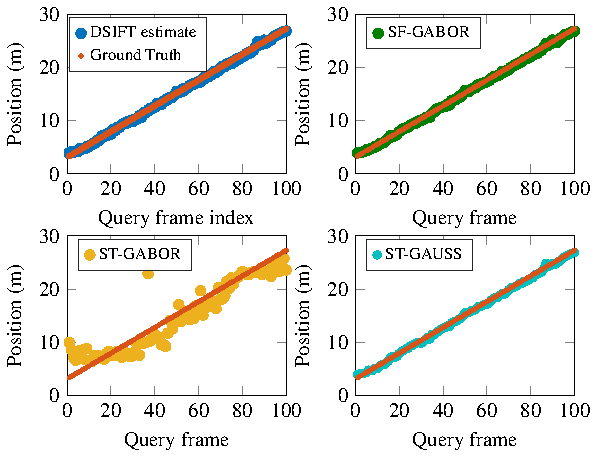
\includegraphics[width=.5\textwidth]{gfx/Chapter05/2x2comp.pdf}
\caption{Sub-APC location estimate comparison. Using broad place-cell tuning curves, very accurate localization can
be achieved within a section of corridor. For this corridor and for this journey,
absolute localization errors range from below one metre to 1.49 m. Ground truth is shown in red. In this case, only \textbf{single-device} (Nexus 4) queries were used. The effect of using queries from both devices is shown in Figure \ref{fig:multiDevice} and captured by Table~\ref{table:methodComparison}.}
\label{fig:sublocMethodComp}
\end{figure}

\begin{figure}
\centering
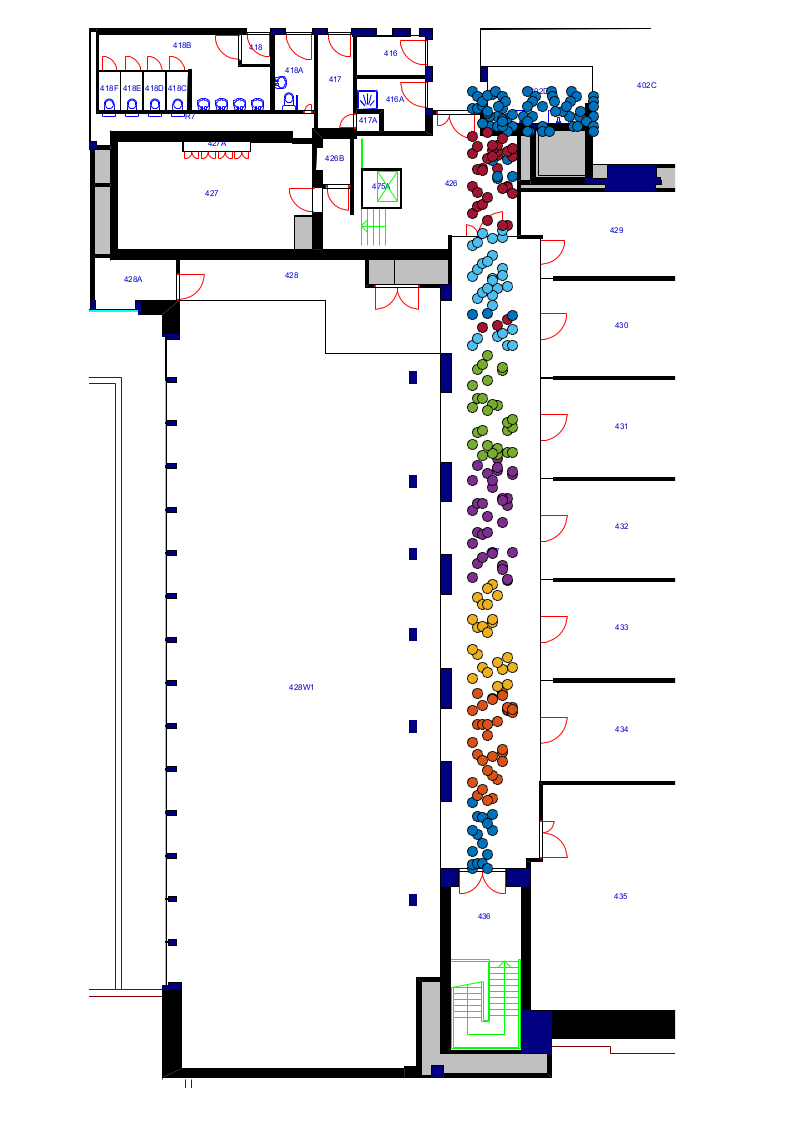
\includegraphics[height=\linewidth]{gfx/Chapter05/placeCellsExperiment_withDetection_5px.png}
\caption{Using ground truth from a surveyor's wheel, activations from APCs are overlaid onto the floor plan in which video data was acquired. Different colours refer to individual APCs.}
\label{fig:floorplan}
\end{figure}

\subsection{Parameter Tuning}

%% Subfigure in tikz
%\begin{figure}[t]
%\begin{subfigure}[]{
%%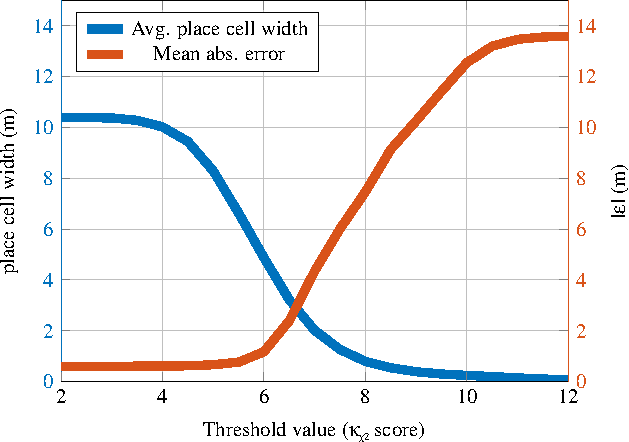
\includegraphics[width=.4\textwidth, height=.3\textwidth]{gfx/Chapter05/errorWidthEvalDSIFT_16pc.pdf}
%	\setlength\figureheight{0.25\linewidth}
%	\setlength\figurewidth{0.35\linewidth}
%		% This file was created by matlab2tikz.
% Minimal pgfplots version: 1.3
%
%The latest updates can be retrieved from
%  http://www.mathworks.com/matlabcentral/fileexchange/22022-matlab2tikz
%where you can also make suggestions and rate matlab2tikz.
%
\definecolor{mycolor1}{rgb}{0.00000,0.44700,0.74100}%
\definecolor{mycolor2}{rgb}{0.85000,0.32500,0.09800}%
%
\begin{tikzpicture}

\begin{axis}[%
width=1\figurewidth,
height=\figureheight,
at={(0\figurewidth,0\figureheight)},
scale only axis,
xmin=2,
xmax=12,
xlabel={$\text{Threshold value (}\chi{}^\text{2}\text{ score)}$},
xmajorgrids,
separate axis lines,
every outer y axis line/.append style={mycolor1},
every y tick label/.append style={font=\color{mycolor1}},
ymin=0,
ymax=15,
ytick={ 0,  2,  4,  6,  8, 10, 12, 14, 16},
ylabel={place cell width (m)},
ymajorgrids,
%legend style={font=\scriptsize},
legend pos=north west],

\addplot [color=mycolor1,solid,line width=4.0pt]
  table[row sep=crcr]{%
2	10.3823661718399\\
2.5	10.3810683760684\\
3	10.3703615609537\\
3.5	10.2759469185785\\
4	10.0183344579397\\
4.5	9.44243758434548\\
5	8.2841548582996\\
5.5	6.62719410706253\\
6	4.86835638776428\\
6.5	3.20912449392713\\
7	2.00898785425101\\
7.5	1.25691520467836\\
8	0.789384278002699\\
8.5	0.537287449392713\\
9	0.383498650472335\\
9.5	0.294599640125956\\
10	0.239767768780927\\
10.5	0.194344916779127\\
11	0.142108636977058\\
11.5	0.0976591318038686\\
12	0.0671609311740891\\
};
\addlegendentry{Avg. place cell width};

\addplot [color=mycolor2,solid,line width=4.0pt]
  table[row sep=crcr]{%
2	0.59827997230238\\
2.5	0.598283303449651\\
3	0.59853210334464\\
3.5	0.604599771139626\\
4	0.611538255558397\\
4.5	0.616405904188176\\
5	0.659590799301437\\
5.5	0.761593198038283\\
6	1.16969392265532\\
6.5	2.39061659899491\\
7	4.35209908745593\\
7.5	6.01339962013322\\
8	7.46592916884236\\
8.5	9.13823310685466\\
9	10.258035806541\\
9.5	11.4226149894715\\
10	12.5487583603638\\
10.5	13.1969679693367\\
11	13.4649228770933\\
11.5	13.5563611613463\\
12	13.583758620106\\
};
\addlegendentry{Mean abs. error};

\end{axis}

\begin{axis}[%
width=1\figurewidth,
height=\figureheight,
at={(0\figurewidth,0\figureheight)},
scale only axis,
xmin=2,
xmax=12,
every outer y axis line/.append style={mycolor2},
every y tick label/.append style={font=\color{mycolor2}},
ymin=0,
ymax=15,
ytick={ 0,  2,  4,  6,  8, 10, 12, 14, 16},
ylabel={$\text{|}\epsilon\text{| (m)}$},
axis x line*=bottom,
axis y line*=right
]


\end{axis}
\end{tikzpicture}%
%
%}\label{fig:threshEval}
%\end{subfigure}
%~
%\begin{subfigure}[]{
%	\setlength\figureheight{0.25\linewidth}
%	\setlength\figurewidth{0.35\linewidth}
%		% This file was created by matlab2tikz.
% Minimal pgfplots version: 1.3
%
%The latest updates can be retrieved from
%  http://www.mathworks.com/matlabcentral/fileexchange/22022-matlab2tikz
%where you can also make suggestions and rate matlab2tikz.
%
\definecolor{mycolor1}{rgb}{0.00000,0.49804,0.00000}%
\definecolor{mycolor2}{rgb}{0.85000,0.32500,0.09800}%
\definecolor{mycolor3}{rgb}{0.00000,0.44700,0.74100}%
\definecolor{mycolor4}{rgb}{0.00000,0.44706,0.74118}%
%
\begin{tikzpicture}

\begin{axis}[%
width=\figurewidth,
height=\figureheight,
at={(0\figurewidth,0\figureheight)},
scale only axis,
xmin=0,
xmax=100,
xlabel={Query frame},
ymin=0,
ymax=30,
ylabel={Position (m)},
legend style={at={(0.01,0.98)},anchor=north west,legend cell align=left,align=left,draw=white!15!black},
legend style = {font=\scriptsize}
]
\addplot [color=mycolor1,solid,line width=6.0pt]
  table[row sep=crcr]{%
1	3.95891986122511\\
2	3.99399560343664\\
3	4.01182087523692\\
4	4.0940710070734\\
5	4.33870923980176\\
6	4.51039124941123\\
7	4.77607957034434\\
8	5.03897072650408\\
9	4.82791114666682\\
10	5.17172216855818\\
11	5.48287111131948\\
12	5.68184366595173\\
13	5.93684184409511\\
14	6.45199887963063\\
15	6.57515029265823\\
16	6.9726130113389\\
17	7.07161908120822\\
18	7.06669063719513\\
19	7.55749099410202\\
20	7.88126606786292\\
21	8.2136952847536\\
22	8.56837706991646\\
23	8.65063507180656\\
24	8.99233695426364\\
25	9.13423464862316\\
26	9.36914654550488\\
27	9.54755148228382\\
28	9.61675655396717\\
29	9.90219232891264\\
30	10.0266081478277\\
31	10.1798447750241\\
32	10.4792914492521\\
33	10.7189018963729\\
34	10.7182308516681\\
35	11.0673317620267\\
36	11.6433247403689\\
37	12.0784408006845\\
38	12.2130159980877\\
39	12.4284847467132\\
40	12.6197999703464\\
41	12.6761876861795\\
42	13.0862648128884\\
43	12.926127903674\\
44	13.9231283284257\\
45	13.9750529442556\\
46	14.131285265065\\
47	14.4529061319552\\
48	14.4169010173426\\
49	14.8316700701916\\
50	15.6267245854858\\
51	15.5232608491538\\
52	15.4318666520949\\
53	15.8629566506372\\
54	16.0245114598098\\
55	16.1976025317084\\
56	16.6452611544914\\
57	16.7861319877914\\
58	17.0600963620157\\
59	17.2321080308678\\
60	17.4145722114406\\
61	17.6229069650075\\
62	17.8761197663098\\
63	18.0612136427172\\
64	18.2542643943073\\
65	18.3897012306756\\
66	18.8130577994181\\
67	19.2307613650247\\
68	19.2180947461263\\
69	19.6211395357413\\
70	19.5069672743292\\
71	19.9326492761882\\
72	20.2467468596855\\
73	20.4995201786927\\
74	20.6562338503021\\
75	20.9377969442584\\
76	21.1229762463926\\
77	21.4007778250003\\
78	21.5359536417457\\
79	21.9178044031582\\
80	22.0127558119757\\
81	22.3468702031362\\
82	22.6124574579773\\
83	22.9419273198041\\
84	23.318983691998\\
85	23.3773569313293\\
86	23.6730624407165\\
87	24.3444614727804\\
88	24.1280781608087\\
89	24.3960856017056\\
90	24.9385091937221\\
91	24.7318945582574\\
92	24.6420687435553\\
93	25.1501349727804\\
94	25.596901830051\\
95	25.8307789746188\\
96	26.0481626129853\\
97	26.3191302355823\\
98	26.5642904249671\\
99	26.7207363717027\\
100	26.7580975720235\\
};
\addlegendentry{Nexus};

\addplot [color=mycolor2,solid,line width=3.0pt]
  table[row sep=crcr]{%
1	3.34279475982533\\
2	3.58455648184906\\
3	3.82631820387279\\
4	4.06807992589652\\
5	4.30984164792025\\
6	4.55160336994398\\
7	4.79336509196771\\
8	5.03512681399144\\
9	5.27688853601517\\
10	5.5186502580389\\
11	5.76041198006263\\
12	6.00217370208637\\
13	6.2439354241101\\
14	6.48569714613383\\
15	6.72745886815756\\
16	6.96922059018129\\
17	7.21098231220502\\
18	7.45274403422875\\
19	7.69450575625248\\
20	7.93626747827621\\
21	8.17802920029994\\
22	8.41979092232367\\
23	8.6615526443474\\
24	8.90331436637113\\
25	9.14507608839486\\
26	9.3868378104186\\
27	9.62859953244233\\
28	9.87036125446606\\
29	10.1121229764898\\
30	10.3538846985135\\
31	10.5956464205372\\
32	10.837408142561\\
33	11.0791698645847\\
34	11.3209315866084\\
35	11.5626933086322\\
36	11.8044550306559\\
37	12.0462167526796\\
38	12.2879784747034\\
39	12.5297401967271\\
40	12.7715019187508\\
41	13.0132636407746\\
42	13.2550253627983\\
43	13.496787084822\\
44	13.7385488068457\\
45	13.9803105288695\\
46	14.2220722508932\\
47	14.4638339729169\\
48	14.7055956949407\\
49	14.9473574169644\\
50	15.1891191389881\\
51	15.4308808610119\\
52	15.6726425830356\\
53	15.9144043050593\\
54	16.1561660270831\\
55	16.3979277491068\\
56	16.6396894711305\\
57	16.8814511931542\\
58	17.123212915178\\
59	17.3649746372017\\
60	17.6067363592254\\
61	17.8484980812492\\
62	18.0902598032729\\
63	18.3320215252966\\
64	18.5737832473204\\
65	18.8155449693441\\
66	19.0573066913678\\
67	19.2990684133916\\
68	19.5408301354153\\
69	19.782591857439\\
70	20.0243535794627\\
71	20.2661153014865\\
72	20.5078770235102\\
73	20.7496387455339\\
74	20.9914004675577\\
75	21.2331621895814\\
76	21.4749239116051\\
77	21.7166856336289\\
78	21.9584473556526\\
79	22.2002090776763\\
80	22.4419707997001\\
81	22.6837325217238\\
82	22.9254942437475\\
83	23.1672559657712\\
84	23.409017687795\\
85	23.6507794098187\\
86	23.8925411318424\\
87	24.1343028538662\\
88	24.3760645758899\\
89	24.6178262979136\\
90	24.8595880199374\\
91	25.1013497419611\\
92	25.3431114639848\\
93	25.5848731860086\\
94	25.8266349080323\\
95	26.068396630056\\
96	26.3101583520797\\
97	26.5519200741035\\
98	26.7936817961272\\
99	27.0354435181509\\
100	27.2772052401747\\
};
\addlegendentry{Ground truth};

\addplot [color=mycolor3,solid,line width=4.0pt]
  table[row sep=crcr]{%
1	6.60007066449637\\
2	5.92785272863095\\
3	5.687016186299\\
4	5.92559913218094\\
5	6.0679420157205\\
6	6.03743234664135\\
7	6.16775404769092\\
8	6.44713567292414\\
9	6.15692039231835\\
10	5.88574701111935\\
11	6.15520570572298\\
12	5.98996537235879\\
13	6.33900384615836\\
14	6.61093820812671\\
15	6.54125469652764\\
16	6.25309336241928\\
17	6.38495092262213\\
18	6.09278085436858\\
19	5.51028387344236\\
20	5.64074014658715\\
21	5.20719298704229\\
22	5.04521470677486\\
23	5.23492817774981\\
24	5.12826077683126\\
25	5.37667714599612\\
26	5.33323400554014\\
27	5.26406552272163\\
28	5.86606753442397\\
29	5.94603900273642\\
30	6.08554454939578\\
31	6.17904491666555\\
32	6.46477663246188\\
33	6.87025233953206\\
34	6.91700090201438\\
35	7.20650588716755\\
36	6.93104754381588\\
37	6.92442256421902\\
38	7.07645510169706\\
39	7.35385824639341\\
40	7.65507093570099\\
41	8.17326957024826\\
42	8.23496087680646\\
43	8.38977155668106\\
44	8.64354104730036\\
45	8.80669014498272\\
46	8.97169461798206\\
47	9.20643562484032\\
48	9.58109914205457\\
49	9.78448971912041\\
50	10.1578065848913\\
51	10.4845409495715\\
52	10.9761700423979\\
53	11.1434477351136\\
54	11.2262009634603\\
55	11.1278414031789\\
56	11.272641491395\\
57	11.4380987314461\\
58	11.4968572413094\\
59	11.5201090785929\\
60	11.8669160882775\\
61	12.3998687484535\\
62	13.0714477131908\\
63	13.1342480049515\\
64	13.3951701190543\\
65	13.6550159706449\\
66	13.7013574969606\\
67	13.8434135671891\\
68	14.2401976521718\\
69	14.343539171827\\
70	14.6439397085819\\
71	14.6374835164512\\
72	14.6595088084177\\
73	14.916188338885\\
74	15.1772655235273\\
75	15.6368235224048\\
76	15.9849261977759\\
77	16.2688939868069\\
78	16.3675735941432\\
79	16.5615102707145\\
80	17.4331645440274\\
81	18.3865035154062\\
82	18.6508641695665\\
83	18.8562009631024\\
84	18.8007726564535\\
85	19.3789978255611\\
86	19.2686529763252\\
87	19.5783950949006\\
88	20.0798032349941\\
89	20.2415679426323\\
90	20.7626980843828\\
91	21.0474763083756\\
92	21.3819044479592\\
93	21.8536226846781\\
94	22.1607639679385\\
95	22.251562202227\\
96	22.3160889146854\\
97	22.7831067142131\\
98	23.0921292110273\\
99	23.4447809266646\\
100	23.7845125676908\\
};
\addlegendentry{Glass mean};


\addplot[area legend,solid,fill=mycolor3,opacity=3.000000e-01,draw=mycolor4]
table[row sep=crcr] {%
x	y\\
1	7.73412820780529\\
2	6.46008593978106\\
3	6.24570146764551\\
4	7.29210322975716\\
5	7.25327150684182\\
6	6.54486160704458\\
7	7.03779319034372\\
8	7.34879236124054\\
9	7.41660191494291\\
10	7.35492497616437\\
11	7.38193676636496\\
12	6.69847549415211\\
13	7.2779134985469\\
14	7.39196061617373\\
15	7.36795479599505\\
16	7.42824516054176\\
17	7.41247246950517\\
18	7.52329907678671\\
19	7.59271384572131\\
20	7.27911867367687\\
21	6.63016000220822\\
22	6.57345686552689\\
23	6.85455358468738\\
24	7.06462860466788\\
25	7.39664768171646\\
26	7.55107405558367\\
27	7.52156069007927\\
28	7.78607471566311\\
29	7.86090072428763\\
30	8.24411576174922\\
31	8.77897782450524\\
32	9.22623927303958\\
33	9.49546801345657\\
34	10.0923925106626\\
35	10.1212112009927\\
36	10.2772631380113\\
37	10.2975665555991\\
38	10.444478534911\\
39	10.6624239912627\\
40	10.8427667308095\\
41	11.0785722822543\\
42	11.2515172685256\\
43	11.2467567705391\\
44	11.3773547124529\\
45	11.51379332723\\
46	11.7234146703815\\
47	12.0337234358969\\
48	12.3653105953823\\
49	11.8992300966019\\
50	12.3685813011412\\
51	12.3675657829514\\
52	12.771883450222\\
53	13.3535734592886\\
54	13.6524478518153\\
55	12.7894838277191\\
56	13.2959792824136\\
57	13.0429068244449\\
58	12.8245775828429\\
59	12.8850186295404\\
60	13.2027971210055\\
61	13.5362838959773\\
62	15.9117868063825\\
63	16.7334534855716\\
64	16.9158695714149\\
65	17.3343526009011\\
66	17.2019155414117\\
67	17.6944439783175\\
68	17.7321351459827\\
69	17.936291084189\\
70	18.0793110771903\\
71	18.4455993039802\\
72	18.8468025734908\\
73	18.9753928113467\\
74	19.4395217991717\\
75	19.7286883250655\\
76	19.872271444612\\
77	20.1496712171316\\
78	20.1765730336345\\
79	20.5963537534297\\
80	21.3120132544807\\
81	21.2857865798661\\
82	21.4343603625766\\
83	21.434554552565\\
84	21.3306596962195\\
85	23.4098020139203\\
86	23.165782815752\\
87	23.3951647843391\\
88	23.3683509237006\\
89	23.7152978124534\\
90	24.3178604565234\\
91	24.4039883153834\\
92	25.0364421745563\\
93	25.2751430492186\\
94	25.7820623017502\\
95	25.786441065874\\
96	25.8046791393274\\
97	25.7153471766671\\
98	25.8831813828597\\
99	25.9367577886048\\
100	26.2288454586551\\
100	21.2577579232529\\
99	21.2359685287324\\
98	21.188020733019\\
97	20.7205003133693\\
96	20.2938192684016\\
95	20.1340533226703\\
94	20.0624986711389\\
93	19.9389242531869\\
92	19.1229016369849\\
91	19.1876537262629\\
90	18.5223801036643\\
89	18.3380218532371\\
88	17.8179115204368\\
87	17.7693255414815\\
86	17.3235167923889\\
85	17.0413005020994\\
84	16.6645490072101\\
83	17.0366785377054\\
82	16.8348008882211\\
81	15.3622189049895\\
80	14.9635824014381\\
79	14.1472398318235\\
78	13.4214788327246\\
77	14.0769279363373\\
76	13.8390043890546\\
75	12.9888534351674\\
74	12.3845906351382\\
73	12.4311219641638\\
72	12.2734593073493\\
71	12.3543594207083\\
70	12.4058084635794\\
69	11.98027497285\\
68	12.0180839883129\\
67	11.9504757245858\\
66	12.0023099532419\\
65	11.9872677729365\\
64	12.0727453440006\\
63	11.3284514363209\\
62	11.7415416954665\\
61	11.1861409385136\\
60	10.6736516450915\\
59	10.584001077797\\
58	10.5667011008712\\
57	10.378848187089\\
56	10.3421082618895\\
55	10.2108319075599\\
54	10.1356361968936\\
53	10.1576285660407\\
52	9.84523160030064\\
51	9.50463070165009\\
50	8.93882158297014\\
49	8.0613124594864\\
48	7.91589237203748\\
47	7.61474315382678\\
46	7.49302648921106\\
45	7.02349157152528\\
44	6.69290470034223\\
43	6.2562569191854\\
42	6.12586951040475\\
41	6.24862168023871\\
40	5.48777496327747\\
39	5.33576804137469\\
38	5.50915818159829\\
37	5.1911702786603\\
36	5.33041553762058\\
35	5.4295228597455\\
34	5.46208583020652\\
33	5.48338487476781\\
32	5.09402427759154\\
31	4.56621926749042\\
30	4.44064773496236\\
29	4.42387517147249\\
28	4.3831792723988\\
27	4.35365911763364\\
26	4.36567916041625\\
25	4.32358237356421\\
24	4.35792773351444\\
23	4.20194827646796\\
22	3.85065643409124\\
21	3.58020419053268\\
20	3.77739704289719\\
19	4.39071308247044\\
18	4.39070702700026\\
17	4.30413878807365\\
16	4.47006269626111\\
15	4.79110446848886\\
14	5.10585760466108\\
13	4.51216253198812\\
12	4.18571281444878\\
11	4.32823168230603\\
10	4.08512146396065\\
9	4.34062752626781\\
8	4.38992827688547\\
7	4.3886057087822\\
6	4.87372280862943\\
5	4.26341552552919\\
4	4.17922581289768\\
3	3.99144124131088\\
2	4.30352024328658\\
1	6.01778472286323\\
}--cycle;

\addlegendentry{Glass variability};

\end{axis}
\end{tikzpicture}%
%		}
%\label{fig:multiDevice}
%\end{subfigure}
%\caption{Multi}
%\label{fig:}
%\end{figure}



The GRNN relied on the overlap of the responses of the place cells to perform location inference. By varying the threshold beyond which place cells are considered active, it is possible to have very long-tailed APC responses, spanning several metres.  This yields APC behaviour that is similar to that of rate-coding in place cells observed in biology. The blue trace on Fig.~\ref{fig:threshEval} shows an example of the average cell width in metres as the threshold on the $\kappa_{\chi^2}$ comparison metric is varied. The red trace illustrates the average error, also in metres, that is obtained from the GRNN regressor. Having low APC response overlap deprives the network of sufficient non-zero inputs, leading to poor accuracy in position inference.


One of the key problems with using different cameras -- even if they are calibrated -- is the difference in field of view of one imaging device with respect to another.  A Nexus 4 smartphone and a wearable Google Glass were used to conduct experiments into the effect of the dictionary on the localisation using the sub-APC (GRNN) approach. 

A set of 10 journeys through one of the corridors of the RSM building with different devices was taken for this experiment.  Some of the journeys were included in the database, others were used to conduct queries.  The partitioning of the data was permuted, varying the number of journeys in the database and the number of query journeys kept out of the database.  Journeys which were used for queries did not contribute to the learning of the dictionary, which was repeated for each permutation. Fig. \ref{fig:multiDevice}  shows the difference in absolute error of Nexus and Glass queries when only passes from one device (in this case, the Nexus) were used for the dictionary learning. 


\begin{figure}[h!]
\centering
%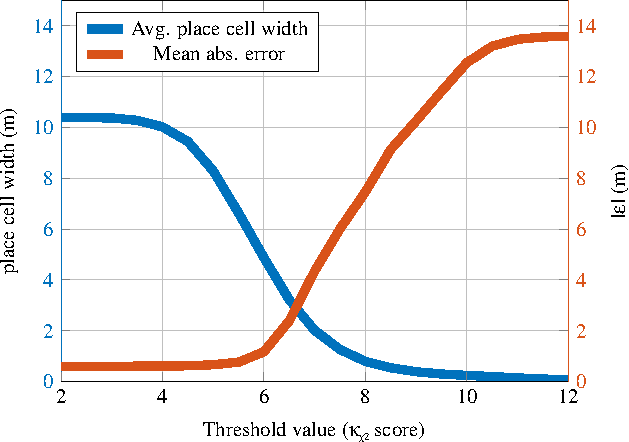
\includegraphics[width=\textwidth]{gfx/Chapter05/errorWidthEvalDSIFT_16pc.pdf}
\setlength\figureheight{0.6\textwidth}
	\setlength\figurewidth{0.8\linewidth} % This file was created by matlab2tikz.
% Minimal pgfplots version: 1.3
%
%The latest updates can be retrieved from
%  http://www.mathworks.com/matlabcentral/fileexchange/22022-matlab2tikz
%where you can also make suggestions and rate matlab2tikz.
%
\definecolor{mycolor1}{rgb}{0.00000,0.44700,0.74100}%
\definecolor{mycolor2}{rgb}{0.85000,0.32500,0.09800}%
%
\begin{tikzpicture}

\begin{axis}[%
width=1\figurewidth,
height=\figureheight,
at={(0\figurewidth,0\figureheight)},
scale only axis,
xmin=2,
xmax=12,
xlabel={$\text{Threshold value (}\chi{}^\text{2}\text{ score)}$},
xmajorgrids,
separate axis lines,
every outer y axis line/.append style={mycolor1},
every y tick label/.append style={font=\color{mycolor1}},
ymin=0,
ymax=15,
ytick={ 0,  2,  4,  6,  8, 10, 12, 14, 16},
ylabel={place cell width (m)},
ymajorgrids,
%legend style={font=\scriptsize},
legend pos=north west],

\addplot [color=mycolor1,solid,line width=4.0pt]
  table[row sep=crcr]{%
2	10.3823661718399\\
2.5	10.3810683760684\\
3	10.3703615609537\\
3.5	10.2759469185785\\
4	10.0183344579397\\
4.5	9.44243758434548\\
5	8.2841548582996\\
5.5	6.62719410706253\\
6	4.86835638776428\\
6.5	3.20912449392713\\
7	2.00898785425101\\
7.5	1.25691520467836\\
8	0.789384278002699\\
8.5	0.537287449392713\\
9	0.383498650472335\\
9.5	0.294599640125956\\
10	0.239767768780927\\
10.5	0.194344916779127\\
11	0.142108636977058\\
11.5	0.0976591318038686\\
12	0.0671609311740891\\
};
\addlegendentry{Avg. place cell width};

\addplot [color=mycolor2,solid,line width=4.0pt]
  table[row sep=crcr]{%
2	0.59827997230238\\
2.5	0.598283303449651\\
3	0.59853210334464\\
3.5	0.604599771139626\\
4	0.611538255558397\\
4.5	0.616405904188176\\
5	0.659590799301437\\
5.5	0.761593198038283\\
6	1.16969392265532\\
6.5	2.39061659899491\\
7	4.35209908745593\\
7.5	6.01339962013322\\
8	7.46592916884236\\
8.5	9.13823310685466\\
9	10.258035806541\\
9.5	11.4226149894715\\
10	12.5487583603638\\
10.5	13.1969679693367\\
11	13.4649228770933\\
11.5	13.5563611613463\\
12	13.583758620106\\
};
\addlegendentry{Mean abs. error};

\end{axis}

\begin{axis}[%
width=1\figurewidth,
height=\figureheight,
at={(0\figurewidth,0\figureheight)},
scale only axis,
xmin=2,
xmax=12,
every outer y axis line/.append style={mycolor2},
every y tick label/.append style={font=\color{mycolor2}},
ymin=0,
ymax=15,
ytick={ 0,  2,  4,  6,  8, 10, 12, 14, 16},
ylabel={$\text{|}\epsilon\text{| (m)}$},
axis x line*=bottom,
axis y line*=right
]


\end{axis}
\end{tikzpicture}%
\caption{Effect of varying the threshold on place cell width, and therefore overlap and average absolute error in meters.}
\label{fig:threshEval}
\end{figure}


\begin{figure}
\centering
%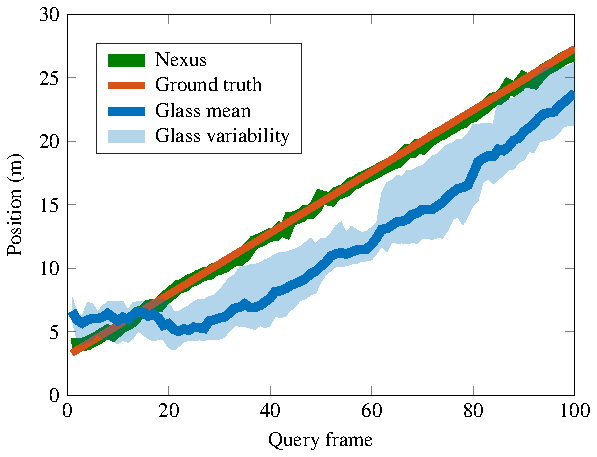
\includegraphics[width=\textwidth]{gfx/Chapter05/nexusVsGlass_sf_gabor_C2.pdf}
\setlength\figureheight{0.6\textwidth}
	\setlength\figurewidth{0.8\linewidth}
		% This file was created by matlab2tikz.
% Minimal pgfplots version: 1.3
%
%The latest updates can be retrieved from
%  http://www.mathworks.com/matlabcentral/fileexchange/22022-matlab2tikz
%where you can also make suggestions and rate matlab2tikz.
%
\definecolor{mycolor1}{rgb}{0.00000,0.49804,0.00000}%
\definecolor{mycolor2}{rgb}{0.85000,0.32500,0.09800}%
\definecolor{mycolor3}{rgb}{0.00000,0.44700,0.74100}%
\definecolor{mycolor4}{rgb}{0.00000,0.44706,0.74118}%
%
\begin{tikzpicture}

\begin{axis}[%
width=\figurewidth,
height=\figureheight,
at={(0\figurewidth,0\figureheight)},
scale only axis,
xmin=0,
xmax=100,
xlabel={Query frame},
ymin=0,
ymax=30,
ylabel={Position (m)},
legend style={at={(0.01,0.98)},anchor=north west,legend cell align=left,align=left,draw=white!15!black},
legend style = {font=\scriptsize}
]
\addplot [color=mycolor1,solid,line width=6.0pt]
  table[row sep=crcr]{%
1	3.95891986122511\\
2	3.99399560343664\\
3	4.01182087523692\\
4	4.0940710070734\\
5	4.33870923980176\\
6	4.51039124941123\\
7	4.77607957034434\\
8	5.03897072650408\\
9	4.82791114666682\\
10	5.17172216855818\\
11	5.48287111131948\\
12	5.68184366595173\\
13	5.93684184409511\\
14	6.45199887963063\\
15	6.57515029265823\\
16	6.9726130113389\\
17	7.07161908120822\\
18	7.06669063719513\\
19	7.55749099410202\\
20	7.88126606786292\\
21	8.2136952847536\\
22	8.56837706991646\\
23	8.65063507180656\\
24	8.99233695426364\\
25	9.13423464862316\\
26	9.36914654550488\\
27	9.54755148228382\\
28	9.61675655396717\\
29	9.90219232891264\\
30	10.0266081478277\\
31	10.1798447750241\\
32	10.4792914492521\\
33	10.7189018963729\\
34	10.7182308516681\\
35	11.0673317620267\\
36	11.6433247403689\\
37	12.0784408006845\\
38	12.2130159980877\\
39	12.4284847467132\\
40	12.6197999703464\\
41	12.6761876861795\\
42	13.0862648128884\\
43	12.926127903674\\
44	13.9231283284257\\
45	13.9750529442556\\
46	14.131285265065\\
47	14.4529061319552\\
48	14.4169010173426\\
49	14.8316700701916\\
50	15.6267245854858\\
51	15.5232608491538\\
52	15.4318666520949\\
53	15.8629566506372\\
54	16.0245114598098\\
55	16.1976025317084\\
56	16.6452611544914\\
57	16.7861319877914\\
58	17.0600963620157\\
59	17.2321080308678\\
60	17.4145722114406\\
61	17.6229069650075\\
62	17.8761197663098\\
63	18.0612136427172\\
64	18.2542643943073\\
65	18.3897012306756\\
66	18.8130577994181\\
67	19.2307613650247\\
68	19.2180947461263\\
69	19.6211395357413\\
70	19.5069672743292\\
71	19.9326492761882\\
72	20.2467468596855\\
73	20.4995201786927\\
74	20.6562338503021\\
75	20.9377969442584\\
76	21.1229762463926\\
77	21.4007778250003\\
78	21.5359536417457\\
79	21.9178044031582\\
80	22.0127558119757\\
81	22.3468702031362\\
82	22.6124574579773\\
83	22.9419273198041\\
84	23.318983691998\\
85	23.3773569313293\\
86	23.6730624407165\\
87	24.3444614727804\\
88	24.1280781608087\\
89	24.3960856017056\\
90	24.9385091937221\\
91	24.7318945582574\\
92	24.6420687435553\\
93	25.1501349727804\\
94	25.596901830051\\
95	25.8307789746188\\
96	26.0481626129853\\
97	26.3191302355823\\
98	26.5642904249671\\
99	26.7207363717027\\
100	26.7580975720235\\
};
\addlegendentry{Nexus};

\addplot [color=mycolor2,solid,line width=3.0pt]
  table[row sep=crcr]{%
1	3.34279475982533\\
2	3.58455648184906\\
3	3.82631820387279\\
4	4.06807992589652\\
5	4.30984164792025\\
6	4.55160336994398\\
7	4.79336509196771\\
8	5.03512681399144\\
9	5.27688853601517\\
10	5.5186502580389\\
11	5.76041198006263\\
12	6.00217370208637\\
13	6.2439354241101\\
14	6.48569714613383\\
15	6.72745886815756\\
16	6.96922059018129\\
17	7.21098231220502\\
18	7.45274403422875\\
19	7.69450575625248\\
20	7.93626747827621\\
21	8.17802920029994\\
22	8.41979092232367\\
23	8.6615526443474\\
24	8.90331436637113\\
25	9.14507608839486\\
26	9.3868378104186\\
27	9.62859953244233\\
28	9.87036125446606\\
29	10.1121229764898\\
30	10.3538846985135\\
31	10.5956464205372\\
32	10.837408142561\\
33	11.0791698645847\\
34	11.3209315866084\\
35	11.5626933086322\\
36	11.8044550306559\\
37	12.0462167526796\\
38	12.2879784747034\\
39	12.5297401967271\\
40	12.7715019187508\\
41	13.0132636407746\\
42	13.2550253627983\\
43	13.496787084822\\
44	13.7385488068457\\
45	13.9803105288695\\
46	14.2220722508932\\
47	14.4638339729169\\
48	14.7055956949407\\
49	14.9473574169644\\
50	15.1891191389881\\
51	15.4308808610119\\
52	15.6726425830356\\
53	15.9144043050593\\
54	16.1561660270831\\
55	16.3979277491068\\
56	16.6396894711305\\
57	16.8814511931542\\
58	17.123212915178\\
59	17.3649746372017\\
60	17.6067363592254\\
61	17.8484980812492\\
62	18.0902598032729\\
63	18.3320215252966\\
64	18.5737832473204\\
65	18.8155449693441\\
66	19.0573066913678\\
67	19.2990684133916\\
68	19.5408301354153\\
69	19.782591857439\\
70	20.0243535794627\\
71	20.2661153014865\\
72	20.5078770235102\\
73	20.7496387455339\\
74	20.9914004675577\\
75	21.2331621895814\\
76	21.4749239116051\\
77	21.7166856336289\\
78	21.9584473556526\\
79	22.2002090776763\\
80	22.4419707997001\\
81	22.6837325217238\\
82	22.9254942437475\\
83	23.1672559657712\\
84	23.409017687795\\
85	23.6507794098187\\
86	23.8925411318424\\
87	24.1343028538662\\
88	24.3760645758899\\
89	24.6178262979136\\
90	24.8595880199374\\
91	25.1013497419611\\
92	25.3431114639848\\
93	25.5848731860086\\
94	25.8266349080323\\
95	26.068396630056\\
96	26.3101583520797\\
97	26.5519200741035\\
98	26.7936817961272\\
99	27.0354435181509\\
100	27.2772052401747\\
};
\addlegendentry{Ground truth};

\addplot [color=mycolor3,solid,line width=4.0pt]
  table[row sep=crcr]{%
1	6.60007066449637\\
2	5.92785272863095\\
3	5.687016186299\\
4	5.92559913218094\\
5	6.0679420157205\\
6	6.03743234664135\\
7	6.16775404769092\\
8	6.44713567292414\\
9	6.15692039231835\\
10	5.88574701111935\\
11	6.15520570572298\\
12	5.98996537235879\\
13	6.33900384615836\\
14	6.61093820812671\\
15	6.54125469652764\\
16	6.25309336241928\\
17	6.38495092262213\\
18	6.09278085436858\\
19	5.51028387344236\\
20	5.64074014658715\\
21	5.20719298704229\\
22	5.04521470677486\\
23	5.23492817774981\\
24	5.12826077683126\\
25	5.37667714599612\\
26	5.33323400554014\\
27	5.26406552272163\\
28	5.86606753442397\\
29	5.94603900273642\\
30	6.08554454939578\\
31	6.17904491666555\\
32	6.46477663246188\\
33	6.87025233953206\\
34	6.91700090201438\\
35	7.20650588716755\\
36	6.93104754381588\\
37	6.92442256421902\\
38	7.07645510169706\\
39	7.35385824639341\\
40	7.65507093570099\\
41	8.17326957024826\\
42	8.23496087680646\\
43	8.38977155668106\\
44	8.64354104730036\\
45	8.80669014498272\\
46	8.97169461798206\\
47	9.20643562484032\\
48	9.58109914205457\\
49	9.78448971912041\\
50	10.1578065848913\\
51	10.4845409495715\\
52	10.9761700423979\\
53	11.1434477351136\\
54	11.2262009634603\\
55	11.1278414031789\\
56	11.272641491395\\
57	11.4380987314461\\
58	11.4968572413094\\
59	11.5201090785929\\
60	11.8669160882775\\
61	12.3998687484535\\
62	13.0714477131908\\
63	13.1342480049515\\
64	13.3951701190543\\
65	13.6550159706449\\
66	13.7013574969606\\
67	13.8434135671891\\
68	14.2401976521718\\
69	14.343539171827\\
70	14.6439397085819\\
71	14.6374835164512\\
72	14.6595088084177\\
73	14.916188338885\\
74	15.1772655235273\\
75	15.6368235224048\\
76	15.9849261977759\\
77	16.2688939868069\\
78	16.3675735941432\\
79	16.5615102707145\\
80	17.4331645440274\\
81	18.3865035154062\\
82	18.6508641695665\\
83	18.8562009631024\\
84	18.8007726564535\\
85	19.3789978255611\\
86	19.2686529763252\\
87	19.5783950949006\\
88	20.0798032349941\\
89	20.2415679426323\\
90	20.7626980843828\\
91	21.0474763083756\\
92	21.3819044479592\\
93	21.8536226846781\\
94	22.1607639679385\\
95	22.251562202227\\
96	22.3160889146854\\
97	22.7831067142131\\
98	23.0921292110273\\
99	23.4447809266646\\
100	23.7845125676908\\
};
\addlegendentry{Glass mean};


\addplot[area legend,solid,fill=mycolor3,opacity=3.000000e-01,draw=mycolor4]
table[row sep=crcr] {%
x	y\\
1	7.73412820780529\\
2	6.46008593978106\\
3	6.24570146764551\\
4	7.29210322975716\\
5	7.25327150684182\\
6	6.54486160704458\\
7	7.03779319034372\\
8	7.34879236124054\\
9	7.41660191494291\\
10	7.35492497616437\\
11	7.38193676636496\\
12	6.69847549415211\\
13	7.2779134985469\\
14	7.39196061617373\\
15	7.36795479599505\\
16	7.42824516054176\\
17	7.41247246950517\\
18	7.52329907678671\\
19	7.59271384572131\\
20	7.27911867367687\\
21	6.63016000220822\\
22	6.57345686552689\\
23	6.85455358468738\\
24	7.06462860466788\\
25	7.39664768171646\\
26	7.55107405558367\\
27	7.52156069007927\\
28	7.78607471566311\\
29	7.86090072428763\\
30	8.24411576174922\\
31	8.77897782450524\\
32	9.22623927303958\\
33	9.49546801345657\\
34	10.0923925106626\\
35	10.1212112009927\\
36	10.2772631380113\\
37	10.2975665555991\\
38	10.444478534911\\
39	10.6624239912627\\
40	10.8427667308095\\
41	11.0785722822543\\
42	11.2515172685256\\
43	11.2467567705391\\
44	11.3773547124529\\
45	11.51379332723\\
46	11.7234146703815\\
47	12.0337234358969\\
48	12.3653105953823\\
49	11.8992300966019\\
50	12.3685813011412\\
51	12.3675657829514\\
52	12.771883450222\\
53	13.3535734592886\\
54	13.6524478518153\\
55	12.7894838277191\\
56	13.2959792824136\\
57	13.0429068244449\\
58	12.8245775828429\\
59	12.8850186295404\\
60	13.2027971210055\\
61	13.5362838959773\\
62	15.9117868063825\\
63	16.7334534855716\\
64	16.9158695714149\\
65	17.3343526009011\\
66	17.2019155414117\\
67	17.6944439783175\\
68	17.7321351459827\\
69	17.936291084189\\
70	18.0793110771903\\
71	18.4455993039802\\
72	18.8468025734908\\
73	18.9753928113467\\
74	19.4395217991717\\
75	19.7286883250655\\
76	19.872271444612\\
77	20.1496712171316\\
78	20.1765730336345\\
79	20.5963537534297\\
80	21.3120132544807\\
81	21.2857865798661\\
82	21.4343603625766\\
83	21.434554552565\\
84	21.3306596962195\\
85	23.4098020139203\\
86	23.165782815752\\
87	23.3951647843391\\
88	23.3683509237006\\
89	23.7152978124534\\
90	24.3178604565234\\
91	24.4039883153834\\
92	25.0364421745563\\
93	25.2751430492186\\
94	25.7820623017502\\
95	25.786441065874\\
96	25.8046791393274\\
97	25.7153471766671\\
98	25.8831813828597\\
99	25.9367577886048\\
100	26.2288454586551\\
100	21.2577579232529\\
99	21.2359685287324\\
98	21.188020733019\\
97	20.7205003133693\\
96	20.2938192684016\\
95	20.1340533226703\\
94	20.0624986711389\\
93	19.9389242531869\\
92	19.1229016369849\\
91	19.1876537262629\\
90	18.5223801036643\\
89	18.3380218532371\\
88	17.8179115204368\\
87	17.7693255414815\\
86	17.3235167923889\\
85	17.0413005020994\\
84	16.6645490072101\\
83	17.0366785377054\\
82	16.8348008882211\\
81	15.3622189049895\\
80	14.9635824014381\\
79	14.1472398318235\\
78	13.4214788327246\\
77	14.0769279363373\\
76	13.8390043890546\\
75	12.9888534351674\\
74	12.3845906351382\\
73	12.4311219641638\\
72	12.2734593073493\\
71	12.3543594207083\\
70	12.4058084635794\\
69	11.98027497285\\
68	12.0180839883129\\
67	11.9504757245858\\
66	12.0023099532419\\
65	11.9872677729365\\
64	12.0727453440006\\
63	11.3284514363209\\
62	11.7415416954665\\
61	11.1861409385136\\
60	10.6736516450915\\
59	10.584001077797\\
58	10.5667011008712\\
57	10.378848187089\\
56	10.3421082618895\\
55	10.2108319075599\\
54	10.1356361968936\\
53	10.1576285660407\\
52	9.84523160030064\\
51	9.50463070165009\\
50	8.93882158297014\\
49	8.0613124594864\\
48	7.91589237203748\\
47	7.61474315382678\\
46	7.49302648921106\\
45	7.02349157152528\\
44	6.69290470034223\\
43	6.2562569191854\\
42	6.12586951040475\\
41	6.24862168023871\\
40	5.48777496327747\\
39	5.33576804137469\\
38	5.50915818159829\\
37	5.1911702786603\\
36	5.33041553762058\\
35	5.4295228597455\\
34	5.46208583020652\\
33	5.48338487476781\\
32	5.09402427759154\\
31	4.56621926749042\\
30	4.44064773496236\\
29	4.42387517147249\\
28	4.3831792723988\\
27	4.35365911763364\\
26	4.36567916041625\\
25	4.32358237356421\\
24	4.35792773351444\\
23	4.20194827646796\\
22	3.85065643409124\\
21	3.58020419053268\\
20	3.77739704289719\\
19	4.39071308247044\\
18	4.39070702700026\\
17	4.30413878807365\\
16	4.47006269626111\\
15	4.79110446848886\\
14	5.10585760466108\\
13	4.51216253198812\\
12	4.18571281444878\\
11	4.32823168230603\\
10	4.08512146396065\\
9	4.34062752626781\\
8	4.38992827688547\\
7	4.3886057087822\\
6	4.87372280862943\\
5	4.26341552552919\\
4	4.17922581289768\\
3	3.99144124131088\\
2	4.30352024328658\\
1	6.01778472286323\\
}--cycle;

\addlegendentry{Glass variability};

\end{axis}
\end{tikzpicture}%
\caption{Multi-device sub-APC localization test.}
\label{fig:multiDevice}
\end{figure}


%\begin{figure}[t]
%\centering
%\subfloat[][Our figure]{\setlength\figureheight{0.6\textwidth}
%	\setlength\figurewidth{0.8\linewidth} % This file was created by matlab2tikz.
% Minimal pgfplots version: 1.3
%
%The latest updates can be retrieved from
%  http://www.mathworks.com/matlabcentral/fileexchange/22022-matlab2tikz
%where you can also make suggestions and rate matlab2tikz.
%
\definecolor{mycolor1}{rgb}{0.00000,0.44700,0.74100}%
\definecolor{mycolor2}{rgb}{0.85000,0.32500,0.09800}%
%
\begin{tikzpicture}

\begin{axis}[%
width=1\figurewidth,
height=\figureheight,
at={(0\figurewidth,0\figureheight)},
scale only axis,
xmin=2,
xmax=12,
xlabel={$\text{Threshold value (}\chi{}^\text{2}\text{ score)}$},
xmajorgrids,
separate axis lines,
every outer y axis line/.append style={mycolor1},
every y tick label/.append style={font=\color{mycolor1}},
ymin=0,
ymax=15,
ytick={ 0,  2,  4,  6,  8, 10, 12, 14, 16},
ylabel={place cell width (m)},
ymajorgrids,
%legend style={font=\scriptsize},
legend pos=north west],

\addplot [color=mycolor1,solid,line width=4.0pt]
  table[row sep=crcr]{%
2	10.3823661718399\\
2.5	10.3810683760684\\
3	10.3703615609537\\
3.5	10.2759469185785\\
4	10.0183344579397\\
4.5	9.44243758434548\\
5	8.2841548582996\\
5.5	6.62719410706253\\
6	4.86835638776428\\
6.5	3.20912449392713\\
7	2.00898785425101\\
7.5	1.25691520467836\\
8	0.789384278002699\\
8.5	0.537287449392713\\
9	0.383498650472335\\
9.5	0.294599640125956\\
10	0.239767768780927\\
10.5	0.194344916779127\\
11	0.142108636977058\\
11.5	0.0976591318038686\\
12	0.0671609311740891\\
};
\addlegendentry{Avg. place cell width};

\addplot [color=mycolor2,solid,line width=4.0pt]
  table[row sep=crcr]{%
2	0.59827997230238\\
2.5	0.598283303449651\\
3	0.59853210334464\\
3.5	0.604599771139626\\
4	0.611538255558397\\
4.5	0.616405904188176\\
5	0.659590799301437\\
5.5	0.761593198038283\\
6	1.16969392265532\\
6.5	2.39061659899491\\
7	4.35209908745593\\
7.5	6.01339962013322\\
8	7.46592916884236\\
8.5	9.13823310685466\\
9	10.258035806541\\
9.5	11.4226149894715\\
10	12.5487583603638\\
10.5	13.1969679693367\\
11	13.4649228770933\\
11.5	13.5563611613463\\
12	13.583758620106\\
};
\addlegendentry{Mean abs. error};

\end{axis}

\begin{axis}[%
width=1\figurewidth,
height=\figureheight,
at={(0\figurewidth,0\figureheight)},
scale only axis,
xmin=2,
xmax=12,
every outer y axis line/.append style={mycolor2},
every y tick label/.append style={font=\color{mycolor2}},
ymin=0,
ymax=15,
ytick={ 0,  2,  4,  6,  8, 10, 12, 14, 16},
ylabel={$\text{|}\epsilon\text{| (m)}$},
axis x line*=bottom,
axis y line*=right
]


\end{axis}
\end{tikzpicture}%
%}\label{fig:threshEval}
%\subfloat[][Our figure]{\setlength\figureheight{0.6\textwidth}
%	\setlength\figurewidth{0.8\linewidth}
%		% This file was created by matlab2tikz.
% Minimal pgfplots version: 1.3
%
%The latest updates can be retrieved from
%  http://www.mathworks.com/matlabcentral/fileexchange/22022-matlab2tikz
%where you can also make suggestions and rate matlab2tikz.
%
\definecolor{mycolor1}{rgb}{0.00000,0.49804,0.00000}%
\definecolor{mycolor2}{rgb}{0.85000,0.32500,0.09800}%
\definecolor{mycolor3}{rgb}{0.00000,0.44700,0.74100}%
\definecolor{mycolor4}{rgb}{0.00000,0.44706,0.74118}%
%
\begin{tikzpicture}

\begin{axis}[%
width=\figurewidth,
height=\figureheight,
at={(0\figurewidth,0\figureheight)},
scale only axis,
xmin=0,
xmax=100,
xlabel={Query frame},
ymin=0,
ymax=30,
ylabel={Position (m)},
legend style={at={(0.01,0.98)},anchor=north west,legend cell align=left,align=left,draw=white!15!black},
legend style = {font=\scriptsize}
]
\addplot [color=mycolor1,solid,line width=6.0pt]
  table[row sep=crcr]{%
1	3.95891986122511\\
2	3.99399560343664\\
3	4.01182087523692\\
4	4.0940710070734\\
5	4.33870923980176\\
6	4.51039124941123\\
7	4.77607957034434\\
8	5.03897072650408\\
9	4.82791114666682\\
10	5.17172216855818\\
11	5.48287111131948\\
12	5.68184366595173\\
13	5.93684184409511\\
14	6.45199887963063\\
15	6.57515029265823\\
16	6.9726130113389\\
17	7.07161908120822\\
18	7.06669063719513\\
19	7.55749099410202\\
20	7.88126606786292\\
21	8.2136952847536\\
22	8.56837706991646\\
23	8.65063507180656\\
24	8.99233695426364\\
25	9.13423464862316\\
26	9.36914654550488\\
27	9.54755148228382\\
28	9.61675655396717\\
29	9.90219232891264\\
30	10.0266081478277\\
31	10.1798447750241\\
32	10.4792914492521\\
33	10.7189018963729\\
34	10.7182308516681\\
35	11.0673317620267\\
36	11.6433247403689\\
37	12.0784408006845\\
38	12.2130159980877\\
39	12.4284847467132\\
40	12.6197999703464\\
41	12.6761876861795\\
42	13.0862648128884\\
43	12.926127903674\\
44	13.9231283284257\\
45	13.9750529442556\\
46	14.131285265065\\
47	14.4529061319552\\
48	14.4169010173426\\
49	14.8316700701916\\
50	15.6267245854858\\
51	15.5232608491538\\
52	15.4318666520949\\
53	15.8629566506372\\
54	16.0245114598098\\
55	16.1976025317084\\
56	16.6452611544914\\
57	16.7861319877914\\
58	17.0600963620157\\
59	17.2321080308678\\
60	17.4145722114406\\
61	17.6229069650075\\
62	17.8761197663098\\
63	18.0612136427172\\
64	18.2542643943073\\
65	18.3897012306756\\
66	18.8130577994181\\
67	19.2307613650247\\
68	19.2180947461263\\
69	19.6211395357413\\
70	19.5069672743292\\
71	19.9326492761882\\
72	20.2467468596855\\
73	20.4995201786927\\
74	20.6562338503021\\
75	20.9377969442584\\
76	21.1229762463926\\
77	21.4007778250003\\
78	21.5359536417457\\
79	21.9178044031582\\
80	22.0127558119757\\
81	22.3468702031362\\
82	22.6124574579773\\
83	22.9419273198041\\
84	23.318983691998\\
85	23.3773569313293\\
86	23.6730624407165\\
87	24.3444614727804\\
88	24.1280781608087\\
89	24.3960856017056\\
90	24.9385091937221\\
91	24.7318945582574\\
92	24.6420687435553\\
93	25.1501349727804\\
94	25.596901830051\\
95	25.8307789746188\\
96	26.0481626129853\\
97	26.3191302355823\\
98	26.5642904249671\\
99	26.7207363717027\\
100	26.7580975720235\\
};
\addlegendentry{Nexus};

\addplot [color=mycolor2,solid,line width=3.0pt]
  table[row sep=crcr]{%
1	3.34279475982533\\
2	3.58455648184906\\
3	3.82631820387279\\
4	4.06807992589652\\
5	4.30984164792025\\
6	4.55160336994398\\
7	4.79336509196771\\
8	5.03512681399144\\
9	5.27688853601517\\
10	5.5186502580389\\
11	5.76041198006263\\
12	6.00217370208637\\
13	6.2439354241101\\
14	6.48569714613383\\
15	6.72745886815756\\
16	6.96922059018129\\
17	7.21098231220502\\
18	7.45274403422875\\
19	7.69450575625248\\
20	7.93626747827621\\
21	8.17802920029994\\
22	8.41979092232367\\
23	8.6615526443474\\
24	8.90331436637113\\
25	9.14507608839486\\
26	9.3868378104186\\
27	9.62859953244233\\
28	9.87036125446606\\
29	10.1121229764898\\
30	10.3538846985135\\
31	10.5956464205372\\
32	10.837408142561\\
33	11.0791698645847\\
34	11.3209315866084\\
35	11.5626933086322\\
36	11.8044550306559\\
37	12.0462167526796\\
38	12.2879784747034\\
39	12.5297401967271\\
40	12.7715019187508\\
41	13.0132636407746\\
42	13.2550253627983\\
43	13.496787084822\\
44	13.7385488068457\\
45	13.9803105288695\\
46	14.2220722508932\\
47	14.4638339729169\\
48	14.7055956949407\\
49	14.9473574169644\\
50	15.1891191389881\\
51	15.4308808610119\\
52	15.6726425830356\\
53	15.9144043050593\\
54	16.1561660270831\\
55	16.3979277491068\\
56	16.6396894711305\\
57	16.8814511931542\\
58	17.123212915178\\
59	17.3649746372017\\
60	17.6067363592254\\
61	17.8484980812492\\
62	18.0902598032729\\
63	18.3320215252966\\
64	18.5737832473204\\
65	18.8155449693441\\
66	19.0573066913678\\
67	19.2990684133916\\
68	19.5408301354153\\
69	19.782591857439\\
70	20.0243535794627\\
71	20.2661153014865\\
72	20.5078770235102\\
73	20.7496387455339\\
74	20.9914004675577\\
75	21.2331621895814\\
76	21.4749239116051\\
77	21.7166856336289\\
78	21.9584473556526\\
79	22.2002090776763\\
80	22.4419707997001\\
81	22.6837325217238\\
82	22.9254942437475\\
83	23.1672559657712\\
84	23.409017687795\\
85	23.6507794098187\\
86	23.8925411318424\\
87	24.1343028538662\\
88	24.3760645758899\\
89	24.6178262979136\\
90	24.8595880199374\\
91	25.1013497419611\\
92	25.3431114639848\\
93	25.5848731860086\\
94	25.8266349080323\\
95	26.068396630056\\
96	26.3101583520797\\
97	26.5519200741035\\
98	26.7936817961272\\
99	27.0354435181509\\
100	27.2772052401747\\
};
\addlegendentry{Ground truth};

\addplot [color=mycolor3,solid,line width=4.0pt]
  table[row sep=crcr]{%
1	6.60007066449637\\
2	5.92785272863095\\
3	5.687016186299\\
4	5.92559913218094\\
5	6.0679420157205\\
6	6.03743234664135\\
7	6.16775404769092\\
8	6.44713567292414\\
9	6.15692039231835\\
10	5.88574701111935\\
11	6.15520570572298\\
12	5.98996537235879\\
13	6.33900384615836\\
14	6.61093820812671\\
15	6.54125469652764\\
16	6.25309336241928\\
17	6.38495092262213\\
18	6.09278085436858\\
19	5.51028387344236\\
20	5.64074014658715\\
21	5.20719298704229\\
22	5.04521470677486\\
23	5.23492817774981\\
24	5.12826077683126\\
25	5.37667714599612\\
26	5.33323400554014\\
27	5.26406552272163\\
28	5.86606753442397\\
29	5.94603900273642\\
30	6.08554454939578\\
31	6.17904491666555\\
32	6.46477663246188\\
33	6.87025233953206\\
34	6.91700090201438\\
35	7.20650588716755\\
36	6.93104754381588\\
37	6.92442256421902\\
38	7.07645510169706\\
39	7.35385824639341\\
40	7.65507093570099\\
41	8.17326957024826\\
42	8.23496087680646\\
43	8.38977155668106\\
44	8.64354104730036\\
45	8.80669014498272\\
46	8.97169461798206\\
47	9.20643562484032\\
48	9.58109914205457\\
49	9.78448971912041\\
50	10.1578065848913\\
51	10.4845409495715\\
52	10.9761700423979\\
53	11.1434477351136\\
54	11.2262009634603\\
55	11.1278414031789\\
56	11.272641491395\\
57	11.4380987314461\\
58	11.4968572413094\\
59	11.5201090785929\\
60	11.8669160882775\\
61	12.3998687484535\\
62	13.0714477131908\\
63	13.1342480049515\\
64	13.3951701190543\\
65	13.6550159706449\\
66	13.7013574969606\\
67	13.8434135671891\\
68	14.2401976521718\\
69	14.343539171827\\
70	14.6439397085819\\
71	14.6374835164512\\
72	14.6595088084177\\
73	14.916188338885\\
74	15.1772655235273\\
75	15.6368235224048\\
76	15.9849261977759\\
77	16.2688939868069\\
78	16.3675735941432\\
79	16.5615102707145\\
80	17.4331645440274\\
81	18.3865035154062\\
82	18.6508641695665\\
83	18.8562009631024\\
84	18.8007726564535\\
85	19.3789978255611\\
86	19.2686529763252\\
87	19.5783950949006\\
88	20.0798032349941\\
89	20.2415679426323\\
90	20.7626980843828\\
91	21.0474763083756\\
92	21.3819044479592\\
93	21.8536226846781\\
94	22.1607639679385\\
95	22.251562202227\\
96	22.3160889146854\\
97	22.7831067142131\\
98	23.0921292110273\\
99	23.4447809266646\\
100	23.7845125676908\\
};
\addlegendentry{Glass mean};


\addplot[area legend,solid,fill=mycolor3,opacity=3.000000e-01,draw=mycolor4]
table[row sep=crcr] {%
x	y\\
1	7.73412820780529\\
2	6.46008593978106\\
3	6.24570146764551\\
4	7.29210322975716\\
5	7.25327150684182\\
6	6.54486160704458\\
7	7.03779319034372\\
8	7.34879236124054\\
9	7.41660191494291\\
10	7.35492497616437\\
11	7.38193676636496\\
12	6.69847549415211\\
13	7.2779134985469\\
14	7.39196061617373\\
15	7.36795479599505\\
16	7.42824516054176\\
17	7.41247246950517\\
18	7.52329907678671\\
19	7.59271384572131\\
20	7.27911867367687\\
21	6.63016000220822\\
22	6.57345686552689\\
23	6.85455358468738\\
24	7.06462860466788\\
25	7.39664768171646\\
26	7.55107405558367\\
27	7.52156069007927\\
28	7.78607471566311\\
29	7.86090072428763\\
30	8.24411576174922\\
31	8.77897782450524\\
32	9.22623927303958\\
33	9.49546801345657\\
34	10.0923925106626\\
35	10.1212112009927\\
36	10.2772631380113\\
37	10.2975665555991\\
38	10.444478534911\\
39	10.6624239912627\\
40	10.8427667308095\\
41	11.0785722822543\\
42	11.2515172685256\\
43	11.2467567705391\\
44	11.3773547124529\\
45	11.51379332723\\
46	11.7234146703815\\
47	12.0337234358969\\
48	12.3653105953823\\
49	11.8992300966019\\
50	12.3685813011412\\
51	12.3675657829514\\
52	12.771883450222\\
53	13.3535734592886\\
54	13.6524478518153\\
55	12.7894838277191\\
56	13.2959792824136\\
57	13.0429068244449\\
58	12.8245775828429\\
59	12.8850186295404\\
60	13.2027971210055\\
61	13.5362838959773\\
62	15.9117868063825\\
63	16.7334534855716\\
64	16.9158695714149\\
65	17.3343526009011\\
66	17.2019155414117\\
67	17.6944439783175\\
68	17.7321351459827\\
69	17.936291084189\\
70	18.0793110771903\\
71	18.4455993039802\\
72	18.8468025734908\\
73	18.9753928113467\\
74	19.4395217991717\\
75	19.7286883250655\\
76	19.872271444612\\
77	20.1496712171316\\
78	20.1765730336345\\
79	20.5963537534297\\
80	21.3120132544807\\
81	21.2857865798661\\
82	21.4343603625766\\
83	21.434554552565\\
84	21.3306596962195\\
85	23.4098020139203\\
86	23.165782815752\\
87	23.3951647843391\\
88	23.3683509237006\\
89	23.7152978124534\\
90	24.3178604565234\\
91	24.4039883153834\\
92	25.0364421745563\\
93	25.2751430492186\\
94	25.7820623017502\\
95	25.786441065874\\
96	25.8046791393274\\
97	25.7153471766671\\
98	25.8831813828597\\
99	25.9367577886048\\
100	26.2288454586551\\
100	21.2577579232529\\
99	21.2359685287324\\
98	21.188020733019\\
97	20.7205003133693\\
96	20.2938192684016\\
95	20.1340533226703\\
94	20.0624986711389\\
93	19.9389242531869\\
92	19.1229016369849\\
91	19.1876537262629\\
90	18.5223801036643\\
89	18.3380218532371\\
88	17.8179115204368\\
87	17.7693255414815\\
86	17.3235167923889\\
85	17.0413005020994\\
84	16.6645490072101\\
83	17.0366785377054\\
82	16.8348008882211\\
81	15.3622189049895\\
80	14.9635824014381\\
79	14.1472398318235\\
78	13.4214788327246\\
77	14.0769279363373\\
76	13.8390043890546\\
75	12.9888534351674\\
74	12.3845906351382\\
73	12.4311219641638\\
72	12.2734593073493\\
71	12.3543594207083\\
70	12.4058084635794\\
69	11.98027497285\\
68	12.0180839883129\\
67	11.9504757245858\\
66	12.0023099532419\\
65	11.9872677729365\\
64	12.0727453440006\\
63	11.3284514363209\\
62	11.7415416954665\\
61	11.1861409385136\\
60	10.6736516450915\\
59	10.584001077797\\
58	10.5667011008712\\
57	10.378848187089\\
56	10.3421082618895\\
55	10.2108319075599\\
54	10.1356361968936\\
53	10.1576285660407\\
52	9.84523160030064\\
51	9.50463070165009\\
50	8.93882158297014\\
49	8.0613124594864\\
48	7.91589237203748\\
47	7.61474315382678\\
46	7.49302648921106\\
45	7.02349157152528\\
44	6.69290470034223\\
43	6.2562569191854\\
42	6.12586951040475\\
41	6.24862168023871\\
40	5.48777496327747\\
39	5.33576804137469\\
38	5.50915818159829\\
37	5.1911702786603\\
36	5.33041553762058\\
35	5.4295228597455\\
34	5.46208583020652\\
33	5.48338487476781\\
32	5.09402427759154\\
31	4.56621926749042\\
30	4.44064773496236\\
29	4.42387517147249\\
28	4.3831792723988\\
27	4.35365911763364\\
26	4.36567916041625\\
25	4.32358237356421\\
24	4.35792773351444\\
23	4.20194827646796\\
22	3.85065643409124\\
21	3.58020419053268\\
20	3.77739704289719\\
19	4.39071308247044\\
18	4.39070702700026\\
17	4.30413878807365\\
16	4.47006269626111\\
15	4.79110446848886\\
14	5.10585760466108\\
13	4.51216253198812\\
12	4.18571281444878\\
11	4.32823168230603\\
10	4.08512146396065\\
9	4.34062752626781\\
8	4.38992827688547\\
7	4.3886057087822\\
6	4.87372280862943\\
5	4.26341552552919\\
4	4.17922581289768\\
3	3.99144124131088\\
2	4.30352024328658\\
1	6.01778472286323\\
}--cycle;

\addlegendentry{Glass variability};

\end{axis}
\end{tikzpicture}%
%}
%\label{fig:multiDevice}
%\caption{Effect of different parameters.}
%\label{fig:}
%\end{figure}



%\begin{figure}[t]
%\setlength\figureheight{0.6\textwidth}
%	\setlength\figurewidth{0.8\linewidth} 
%	% This file was created by matlab2tikz.
% Minimal pgfplots version: 1.3
%
%The latest updates can be retrieved from
%  http://www.mathworks.com/matlabcentral/fileexchange/22022-matlab2tikz
%where you can also make suggestions and rate matlab2tikz.
%
\definecolor{mycolor1}{rgb}{0.00000,0.44700,0.74100}%
\definecolor{mycolor2}{rgb}{0.85000,0.32500,0.09800}%
%
\begin{tikzpicture}

\begin{axis}[%
width=1\figurewidth,
height=\figureheight,
at={(0\figurewidth,0\figureheight)},
scale only axis,
xmin=2,
xmax=12,
xlabel={$\text{Threshold value (}\chi{}^\text{2}\text{ score)}$},
xmajorgrids,
separate axis lines,
every outer y axis line/.append style={mycolor1},
every y tick label/.append style={font=\color{mycolor1}},
ymin=0,
ymax=15,
ytick={ 0,  2,  4,  6,  8, 10, 12, 14, 16},
ylabel={place cell width (m)},
ymajorgrids,
%legend style={font=\scriptsize},
legend pos=north west],

\addplot [color=mycolor1,solid,line width=4.0pt]
  table[row sep=crcr]{%
2	10.3823661718399\\
2.5	10.3810683760684\\
3	10.3703615609537\\
3.5	10.2759469185785\\
4	10.0183344579397\\
4.5	9.44243758434548\\
5	8.2841548582996\\
5.5	6.62719410706253\\
6	4.86835638776428\\
6.5	3.20912449392713\\
7	2.00898785425101\\
7.5	1.25691520467836\\
8	0.789384278002699\\
8.5	0.537287449392713\\
9	0.383498650472335\\
9.5	0.294599640125956\\
10	0.239767768780927\\
10.5	0.194344916779127\\
11	0.142108636977058\\
11.5	0.0976591318038686\\
12	0.0671609311740891\\
};
\addlegendentry{Avg. place cell width};

\addplot [color=mycolor2,solid,line width=4.0pt]
  table[row sep=crcr]{%
2	0.59827997230238\\
2.5	0.598283303449651\\
3	0.59853210334464\\
3.5	0.604599771139626\\
4	0.611538255558397\\
4.5	0.616405904188176\\
5	0.659590799301437\\
5.5	0.761593198038283\\
6	1.16969392265532\\
6.5	2.39061659899491\\
7	4.35209908745593\\
7.5	6.01339962013322\\
8	7.46592916884236\\
8.5	9.13823310685466\\
9	10.258035806541\\
9.5	11.4226149894715\\
10	12.5487583603638\\
10.5	13.1969679693367\\
11	13.4649228770933\\
11.5	13.5563611613463\\
12	13.583758620106\\
};
\addlegendentry{Mean abs. error};

\end{axis}

\begin{axis}[%
width=1\figurewidth,
height=\figureheight,
at={(0\figurewidth,0\figureheight)},
scale only axis,
xmin=2,
xmax=12,
every outer y axis line/.append style={mycolor2},
every y tick label/.append style={font=\color{mycolor2}},
ymin=0,
ymax=15,
ytick={ 0,  2,  4,  6,  8, 10, 12, 14, 16},
ylabel={$\text{|}\epsilon\text{| (m)}$},
axis x line*=bottom,
axis y line*=right
]


\end{axis}
\end{tikzpicture}%
%\label{fig:threshEval}
%\end{figure}
%
%\begin{figure}
%\setlength\figureheight{0.6\textwidth}
%	\setlength\figurewidth{0.8\linewidth}
%		% This file was created by matlab2tikz.
% Minimal pgfplots version: 1.3
%
%The latest updates can be retrieved from
%  http://www.mathworks.com/matlabcentral/fileexchange/22022-matlab2tikz
%where you can also make suggestions and rate matlab2tikz.
%
\definecolor{mycolor1}{rgb}{0.00000,0.49804,0.00000}%
\definecolor{mycolor2}{rgb}{0.85000,0.32500,0.09800}%
\definecolor{mycolor3}{rgb}{0.00000,0.44700,0.74100}%
\definecolor{mycolor4}{rgb}{0.00000,0.44706,0.74118}%
%
\begin{tikzpicture}

\begin{axis}[%
width=\figurewidth,
height=\figureheight,
at={(0\figurewidth,0\figureheight)},
scale only axis,
xmin=0,
xmax=100,
xlabel={Query frame},
ymin=0,
ymax=30,
ylabel={Position (m)},
legend style={at={(0.01,0.98)},anchor=north west,legend cell align=left,align=left,draw=white!15!black},
legend style = {font=\scriptsize}
]
\addplot [color=mycolor1,solid,line width=6.0pt]
  table[row sep=crcr]{%
1	3.95891986122511\\
2	3.99399560343664\\
3	4.01182087523692\\
4	4.0940710070734\\
5	4.33870923980176\\
6	4.51039124941123\\
7	4.77607957034434\\
8	5.03897072650408\\
9	4.82791114666682\\
10	5.17172216855818\\
11	5.48287111131948\\
12	5.68184366595173\\
13	5.93684184409511\\
14	6.45199887963063\\
15	6.57515029265823\\
16	6.9726130113389\\
17	7.07161908120822\\
18	7.06669063719513\\
19	7.55749099410202\\
20	7.88126606786292\\
21	8.2136952847536\\
22	8.56837706991646\\
23	8.65063507180656\\
24	8.99233695426364\\
25	9.13423464862316\\
26	9.36914654550488\\
27	9.54755148228382\\
28	9.61675655396717\\
29	9.90219232891264\\
30	10.0266081478277\\
31	10.1798447750241\\
32	10.4792914492521\\
33	10.7189018963729\\
34	10.7182308516681\\
35	11.0673317620267\\
36	11.6433247403689\\
37	12.0784408006845\\
38	12.2130159980877\\
39	12.4284847467132\\
40	12.6197999703464\\
41	12.6761876861795\\
42	13.0862648128884\\
43	12.926127903674\\
44	13.9231283284257\\
45	13.9750529442556\\
46	14.131285265065\\
47	14.4529061319552\\
48	14.4169010173426\\
49	14.8316700701916\\
50	15.6267245854858\\
51	15.5232608491538\\
52	15.4318666520949\\
53	15.8629566506372\\
54	16.0245114598098\\
55	16.1976025317084\\
56	16.6452611544914\\
57	16.7861319877914\\
58	17.0600963620157\\
59	17.2321080308678\\
60	17.4145722114406\\
61	17.6229069650075\\
62	17.8761197663098\\
63	18.0612136427172\\
64	18.2542643943073\\
65	18.3897012306756\\
66	18.8130577994181\\
67	19.2307613650247\\
68	19.2180947461263\\
69	19.6211395357413\\
70	19.5069672743292\\
71	19.9326492761882\\
72	20.2467468596855\\
73	20.4995201786927\\
74	20.6562338503021\\
75	20.9377969442584\\
76	21.1229762463926\\
77	21.4007778250003\\
78	21.5359536417457\\
79	21.9178044031582\\
80	22.0127558119757\\
81	22.3468702031362\\
82	22.6124574579773\\
83	22.9419273198041\\
84	23.318983691998\\
85	23.3773569313293\\
86	23.6730624407165\\
87	24.3444614727804\\
88	24.1280781608087\\
89	24.3960856017056\\
90	24.9385091937221\\
91	24.7318945582574\\
92	24.6420687435553\\
93	25.1501349727804\\
94	25.596901830051\\
95	25.8307789746188\\
96	26.0481626129853\\
97	26.3191302355823\\
98	26.5642904249671\\
99	26.7207363717027\\
100	26.7580975720235\\
};
\addlegendentry{Nexus};

\addplot [color=mycolor2,solid,line width=3.0pt]
  table[row sep=crcr]{%
1	3.34279475982533\\
2	3.58455648184906\\
3	3.82631820387279\\
4	4.06807992589652\\
5	4.30984164792025\\
6	4.55160336994398\\
7	4.79336509196771\\
8	5.03512681399144\\
9	5.27688853601517\\
10	5.5186502580389\\
11	5.76041198006263\\
12	6.00217370208637\\
13	6.2439354241101\\
14	6.48569714613383\\
15	6.72745886815756\\
16	6.96922059018129\\
17	7.21098231220502\\
18	7.45274403422875\\
19	7.69450575625248\\
20	7.93626747827621\\
21	8.17802920029994\\
22	8.41979092232367\\
23	8.6615526443474\\
24	8.90331436637113\\
25	9.14507608839486\\
26	9.3868378104186\\
27	9.62859953244233\\
28	9.87036125446606\\
29	10.1121229764898\\
30	10.3538846985135\\
31	10.5956464205372\\
32	10.837408142561\\
33	11.0791698645847\\
34	11.3209315866084\\
35	11.5626933086322\\
36	11.8044550306559\\
37	12.0462167526796\\
38	12.2879784747034\\
39	12.5297401967271\\
40	12.7715019187508\\
41	13.0132636407746\\
42	13.2550253627983\\
43	13.496787084822\\
44	13.7385488068457\\
45	13.9803105288695\\
46	14.2220722508932\\
47	14.4638339729169\\
48	14.7055956949407\\
49	14.9473574169644\\
50	15.1891191389881\\
51	15.4308808610119\\
52	15.6726425830356\\
53	15.9144043050593\\
54	16.1561660270831\\
55	16.3979277491068\\
56	16.6396894711305\\
57	16.8814511931542\\
58	17.123212915178\\
59	17.3649746372017\\
60	17.6067363592254\\
61	17.8484980812492\\
62	18.0902598032729\\
63	18.3320215252966\\
64	18.5737832473204\\
65	18.8155449693441\\
66	19.0573066913678\\
67	19.2990684133916\\
68	19.5408301354153\\
69	19.782591857439\\
70	20.0243535794627\\
71	20.2661153014865\\
72	20.5078770235102\\
73	20.7496387455339\\
74	20.9914004675577\\
75	21.2331621895814\\
76	21.4749239116051\\
77	21.7166856336289\\
78	21.9584473556526\\
79	22.2002090776763\\
80	22.4419707997001\\
81	22.6837325217238\\
82	22.9254942437475\\
83	23.1672559657712\\
84	23.409017687795\\
85	23.6507794098187\\
86	23.8925411318424\\
87	24.1343028538662\\
88	24.3760645758899\\
89	24.6178262979136\\
90	24.8595880199374\\
91	25.1013497419611\\
92	25.3431114639848\\
93	25.5848731860086\\
94	25.8266349080323\\
95	26.068396630056\\
96	26.3101583520797\\
97	26.5519200741035\\
98	26.7936817961272\\
99	27.0354435181509\\
100	27.2772052401747\\
};
\addlegendentry{Ground truth};

\addplot [color=mycolor3,solid,line width=4.0pt]
  table[row sep=crcr]{%
1	6.60007066449637\\
2	5.92785272863095\\
3	5.687016186299\\
4	5.92559913218094\\
5	6.0679420157205\\
6	6.03743234664135\\
7	6.16775404769092\\
8	6.44713567292414\\
9	6.15692039231835\\
10	5.88574701111935\\
11	6.15520570572298\\
12	5.98996537235879\\
13	6.33900384615836\\
14	6.61093820812671\\
15	6.54125469652764\\
16	6.25309336241928\\
17	6.38495092262213\\
18	6.09278085436858\\
19	5.51028387344236\\
20	5.64074014658715\\
21	5.20719298704229\\
22	5.04521470677486\\
23	5.23492817774981\\
24	5.12826077683126\\
25	5.37667714599612\\
26	5.33323400554014\\
27	5.26406552272163\\
28	5.86606753442397\\
29	5.94603900273642\\
30	6.08554454939578\\
31	6.17904491666555\\
32	6.46477663246188\\
33	6.87025233953206\\
34	6.91700090201438\\
35	7.20650588716755\\
36	6.93104754381588\\
37	6.92442256421902\\
38	7.07645510169706\\
39	7.35385824639341\\
40	7.65507093570099\\
41	8.17326957024826\\
42	8.23496087680646\\
43	8.38977155668106\\
44	8.64354104730036\\
45	8.80669014498272\\
46	8.97169461798206\\
47	9.20643562484032\\
48	9.58109914205457\\
49	9.78448971912041\\
50	10.1578065848913\\
51	10.4845409495715\\
52	10.9761700423979\\
53	11.1434477351136\\
54	11.2262009634603\\
55	11.1278414031789\\
56	11.272641491395\\
57	11.4380987314461\\
58	11.4968572413094\\
59	11.5201090785929\\
60	11.8669160882775\\
61	12.3998687484535\\
62	13.0714477131908\\
63	13.1342480049515\\
64	13.3951701190543\\
65	13.6550159706449\\
66	13.7013574969606\\
67	13.8434135671891\\
68	14.2401976521718\\
69	14.343539171827\\
70	14.6439397085819\\
71	14.6374835164512\\
72	14.6595088084177\\
73	14.916188338885\\
74	15.1772655235273\\
75	15.6368235224048\\
76	15.9849261977759\\
77	16.2688939868069\\
78	16.3675735941432\\
79	16.5615102707145\\
80	17.4331645440274\\
81	18.3865035154062\\
82	18.6508641695665\\
83	18.8562009631024\\
84	18.8007726564535\\
85	19.3789978255611\\
86	19.2686529763252\\
87	19.5783950949006\\
88	20.0798032349941\\
89	20.2415679426323\\
90	20.7626980843828\\
91	21.0474763083756\\
92	21.3819044479592\\
93	21.8536226846781\\
94	22.1607639679385\\
95	22.251562202227\\
96	22.3160889146854\\
97	22.7831067142131\\
98	23.0921292110273\\
99	23.4447809266646\\
100	23.7845125676908\\
};
\addlegendentry{Glass mean};


\addplot[area legend,solid,fill=mycolor3,opacity=3.000000e-01,draw=mycolor4]
table[row sep=crcr] {%
x	y\\
1	7.73412820780529\\
2	6.46008593978106\\
3	6.24570146764551\\
4	7.29210322975716\\
5	7.25327150684182\\
6	6.54486160704458\\
7	7.03779319034372\\
8	7.34879236124054\\
9	7.41660191494291\\
10	7.35492497616437\\
11	7.38193676636496\\
12	6.69847549415211\\
13	7.2779134985469\\
14	7.39196061617373\\
15	7.36795479599505\\
16	7.42824516054176\\
17	7.41247246950517\\
18	7.52329907678671\\
19	7.59271384572131\\
20	7.27911867367687\\
21	6.63016000220822\\
22	6.57345686552689\\
23	6.85455358468738\\
24	7.06462860466788\\
25	7.39664768171646\\
26	7.55107405558367\\
27	7.52156069007927\\
28	7.78607471566311\\
29	7.86090072428763\\
30	8.24411576174922\\
31	8.77897782450524\\
32	9.22623927303958\\
33	9.49546801345657\\
34	10.0923925106626\\
35	10.1212112009927\\
36	10.2772631380113\\
37	10.2975665555991\\
38	10.444478534911\\
39	10.6624239912627\\
40	10.8427667308095\\
41	11.0785722822543\\
42	11.2515172685256\\
43	11.2467567705391\\
44	11.3773547124529\\
45	11.51379332723\\
46	11.7234146703815\\
47	12.0337234358969\\
48	12.3653105953823\\
49	11.8992300966019\\
50	12.3685813011412\\
51	12.3675657829514\\
52	12.771883450222\\
53	13.3535734592886\\
54	13.6524478518153\\
55	12.7894838277191\\
56	13.2959792824136\\
57	13.0429068244449\\
58	12.8245775828429\\
59	12.8850186295404\\
60	13.2027971210055\\
61	13.5362838959773\\
62	15.9117868063825\\
63	16.7334534855716\\
64	16.9158695714149\\
65	17.3343526009011\\
66	17.2019155414117\\
67	17.6944439783175\\
68	17.7321351459827\\
69	17.936291084189\\
70	18.0793110771903\\
71	18.4455993039802\\
72	18.8468025734908\\
73	18.9753928113467\\
74	19.4395217991717\\
75	19.7286883250655\\
76	19.872271444612\\
77	20.1496712171316\\
78	20.1765730336345\\
79	20.5963537534297\\
80	21.3120132544807\\
81	21.2857865798661\\
82	21.4343603625766\\
83	21.434554552565\\
84	21.3306596962195\\
85	23.4098020139203\\
86	23.165782815752\\
87	23.3951647843391\\
88	23.3683509237006\\
89	23.7152978124534\\
90	24.3178604565234\\
91	24.4039883153834\\
92	25.0364421745563\\
93	25.2751430492186\\
94	25.7820623017502\\
95	25.786441065874\\
96	25.8046791393274\\
97	25.7153471766671\\
98	25.8831813828597\\
99	25.9367577886048\\
100	26.2288454586551\\
100	21.2577579232529\\
99	21.2359685287324\\
98	21.188020733019\\
97	20.7205003133693\\
96	20.2938192684016\\
95	20.1340533226703\\
94	20.0624986711389\\
93	19.9389242531869\\
92	19.1229016369849\\
91	19.1876537262629\\
90	18.5223801036643\\
89	18.3380218532371\\
88	17.8179115204368\\
87	17.7693255414815\\
86	17.3235167923889\\
85	17.0413005020994\\
84	16.6645490072101\\
83	17.0366785377054\\
82	16.8348008882211\\
81	15.3622189049895\\
80	14.9635824014381\\
79	14.1472398318235\\
78	13.4214788327246\\
77	14.0769279363373\\
76	13.8390043890546\\
75	12.9888534351674\\
74	12.3845906351382\\
73	12.4311219641638\\
72	12.2734593073493\\
71	12.3543594207083\\
70	12.4058084635794\\
69	11.98027497285\\
68	12.0180839883129\\
67	11.9504757245858\\
66	12.0023099532419\\
65	11.9872677729365\\
64	12.0727453440006\\
63	11.3284514363209\\
62	11.7415416954665\\
61	11.1861409385136\\
60	10.6736516450915\\
59	10.584001077797\\
58	10.5667011008712\\
57	10.378848187089\\
56	10.3421082618895\\
55	10.2108319075599\\
54	10.1356361968936\\
53	10.1576285660407\\
52	9.84523160030064\\
51	9.50463070165009\\
50	8.93882158297014\\
49	8.0613124594864\\
48	7.91589237203748\\
47	7.61474315382678\\
46	7.49302648921106\\
45	7.02349157152528\\
44	6.69290470034223\\
43	6.2562569191854\\
42	6.12586951040475\\
41	6.24862168023871\\
40	5.48777496327747\\
39	5.33576804137469\\
38	5.50915818159829\\
37	5.1911702786603\\
36	5.33041553762058\\
35	5.4295228597455\\
34	5.46208583020652\\
33	5.48338487476781\\
32	5.09402427759154\\
31	4.56621926749042\\
30	4.44064773496236\\
29	4.42387517147249\\
28	4.3831792723988\\
27	4.35365911763364\\
26	4.36567916041625\\
25	4.32358237356421\\
24	4.35792773351444\\
23	4.20194827646796\\
22	3.85065643409124\\
21	3.58020419053268\\
20	3.77739704289719\\
19	4.39071308247044\\
18	4.39070702700026\\
17	4.30413878807365\\
16	4.47006269626111\\
15	4.79110446848886\\
14	5.10585760466108\\
13	4.51216253198812\\
12	4.18571281444878\\
11	4.32823168230603\\
10	4.08512146396065\\
9	4.34062752626781\\
8	4.38992827688547\\
7	4.3886057087822\\
6	4.87372280862943\\
5	4.26341552552919\\
4	4.17922581289768\\
3	3.99144124131088\\
2	4.30352024328658\\
1	6.01778472286323\\
}--cycle;

\addlegendentry{Glass variability};

\end{axis}
\end{tikzpicture}%
%\label{fig:multiDevice}
%\caption{Effect of different parameters.}
%\end{figure}


\begin{table}[h]
\centering
\begin{adjustbox}{max width=\textwidth}

    \begin{tabular}{lcccccccc}
    ~		 & \multicolumn{3}{c}{\textbf{Sub-APC Localisation}} & \multicolumn{3}{c}{\textbf{APC-level Localisation}} \\ \hline
    \textbf{Method}        & $\mu_{|\epsilon|}$ (m) & $\sigma_{|\epsilon|}$ (m) & Min (m) & Max (m) & $\mu_{|\epsilon|}$ (m) & $\sigma_{|\epsilon|}$ (m)  &   Min (m) & Max (m) \\ \hline
    SIFT     & 3.42 & 2.72 & 0.38 & 6.47 & 4.48  & 5.14  & 0. 34 &  7.56\\ \hline
    DSIFT    & 2.78 & 2.45 & 0.47 & 6.54  & 4.10 & 5.64 & 0.31 & 6.10 \\ \hline
    SF-GABOR & 2.49 & 2.07 & 0.46 & 5.60 & 4.81  & 7.11 & 0.68  & 8.47 \\ \hline
    ST-GABOR & 7.94 & 5.54 & 2.63 & 10.45 & 9.65 & 9.19 & 3.67 & 13.13\\ \hline
    ST-GAUSS & 3.18 & 2.64 & 0.45 & 7.17 & 3.79  & 5.44 & 0.69  & 8.12 \\ \hline
    $\text{LSD-SLAM}^{(*)}$ & \multicolumn{2}{c}{$\mu_{|\epsilon|}$ = 2.48 m } & \multicolumn{2}{c}{$\sigma_{|\epsilon|}$ = 2.37 m} & Min: 1.21 m &  Max: 3.20 m \\ \hline
    \end{tabular}
\end{adjustbox}
    \caption {Absolute error evaluation when using a larger number (40) of APCs of small spatial support (0.61 m), using \texttt{arg max}() to infer spatial position, in contrast to using fewer (16) but larger APCs with substantial overlap and the regression network (sub-APC). The comparison with a state of the art SLAM method (LSD-SLAM) is also included.$^{(*)}$ LSD-SLAM performance is positively affected by the tracking recovery exception, which reduces the error drift by reseting the odometry calculation and the error of the pose-graph optimisation.}
    \label{table:methodComparison}
\end{table}


\subsection{Computational load metrics}
The main computational load for the place-cell computation is due to the dictionary learning, which enables fast lookup of individual frames -- encoded as a single vector of terms from the vocabulary.  The dictionary is built by randomly selecting 200 frames from each sequence, and randomly selecting 800 examples of the joint spatial-temporal encoding, which consists of $D$-dimensional vectors (see Table~\ref{table:methods}). Dictionary learning takes around 1 hour for approximately 50 video sequences of the whole corridor dataset on a 64 GB machine using 400 words. Once learned, encoding a new frame and looking it up takes less than 200 ms using unoptimized \textit{MATLAB} code. 

\section{Discussion}

One of main the conclusions from the results of the previous section is that those methods that are more closely model biological structures such as SIFT (sparse and dense) and SF-GABOR, achieve best results in the tests we have performed. This section will explore a new formulation for our single-frame Gabor (SF-GABOR) that can simultaneously explain the Gabor filters as plausible models of the simple cells found in the V1 and the first-layer weights yielded from convolutional neural networks successful used in many applications \cite{nlp}, \cite{imagenet} in the past few years.

\subsection{A Convolutional Neural Network (CNN) formulation for SF-GABOR}
\label{sec:tensornotation}

Several authors have pointed to the similarities between spatial filter banks employing oriented band-pass filters \cite{wandell1995foundations},\cite{petrou2008next} -- many of which are implemented using spatial convolution -- and the receptive field patterns found in the primary visual cortex (area V1).  These receptive fields are sensitivity patterns to visual stimuli that can be found within individual neurons \cite{olshausen1997sparse,ringach2002spatial}. 

The recent interest in convolutional neural networks \cite{krizhevsky2012imagenet, ji20133d} builds on over two decades of work into architectures and methods for training \cite{lecun1995convolutional}. Recent results in CNN training tend to converge to yield first-layer weights (filters) that are remarkably similar oriented spatial band-pass filters, and therefore also bear striking resemblance to the receptive fields found in biological visual systems at the level of V1 or equivalent.

To reproduce the behaviour of the pipeline describe in Section \ref{ch05:overview} we used a two-layer feed-forward convolutional neural network (CNN) -- adapted from a model used in computational neuroscience -- to simulate the behaviour of a sheet of tissue in V1 containing just under 200,000 neurons. The first layer of this network represents orientation selective, approximately linear simple cells, and the second layer models a population code for joint position/orientation encoding based on the retinotopic arrangement of oriented cells over a region of cortical tissue.  However, rather than learning the weights from random initialization, neurons were constrained to be orientation selective and with spatially antisymmetric weights about the axis of orientation selectivity (see Figure~\ref{fig:OG}).  We have found it useful to introduce a tensor description of the data structures and the processing involved in this CNN.

\subsection{Tensor Population Model}
Tensors have been suggested as a multi-dimensional representation for convolutional neural networks, specifically for representing the stack of spatial filters that is used to perform spatial convolution. Representing a filter set in this way allows various tensor decompositions to be applied \cite{kolda2009tensor} to reduce the representation into smaller convolution operators. However, a definition for {\em tensor convolution} itself appears lacking from the literature. We identify two operators that -- taken together -- can be very useful concepts for {\em reproducibly} describing the structure of convolutional networks; these are {\em tensor convolution} and {\em permuted tensor convolution}. These are defined next and expanded in Appendix \ref{appendixTensorConv}.

First, we adopt the notation and nomenclature of Kolda \cite{kolda2009tensor}.  We treat tensors as multi-way arrays or multidimensional arrays. The  \textit{order} of a tensor is the number of dimensional indices required to address it; for example, an order 5 tensor $\tens{A}$ may have addressable elements $a_{i_1,i_2,i_3,i_4,i_5}$, with each index varying from 1 to $I_n, n = 1,2,3,4,5$ in integer steps; note that in contrast with Kolda's notation, indices are comma-delimited.  Since each element of the tensor can be restricted to be real-valued, we may consider $\tens{A}$ as lying in $I_1\times I_2\times I_3 \times I_4 \times I_5$- dimensional real space. The \textit{mode} of a tensor refers to the tensor elements simultaneously addressed by one of the indices, and is applied to refer to operations that involve, possibly non-exclusively, a particular one of the indices. 

\begin{definition}{\textit{Tensor Convolution}}  We define the tensor convolution operator in modes $\mathcal{M}$ by the following:
\[
 \overset{\mathcal{M}}{[ \ast ]}: \left (\tens{A},\tens{B}  \right ) \longmapsto \tens{C}
\] 
 where $\mathcal{M}$ is a set of $|\mathcal{M}|$ tuples representing paired indices of $\tens{A}$ and $\tens{B}$ over which the convolution is performed.   These indices associate the modes of the tensors being convolved together.

The tensor convolution operator maps tensor, $\tens{A}$, to an equal- or higher-order tensor $\tens{C}$ by the following:
\begin{eqnarray}
\tens{A} \,\, \overset{\mathcal{M}}{[ \ast ]}\, {\tens{B}} &=& \nonumber \\
& &\sum_{i'_{m_1}},\ldots\,\sum_{i_{M}'}   a_{i_1,i_2,...,i_{m_1}',...,i_{M}',...,i_{N_{\tens{A}}}} \times \nonumber \\
& &b_{i_1,i_2,...,i_{n_1}-i_{m_1}',...,i_{n_M}-i_{m_M}',...,i_{N_{\tens{B}}}}
\label{eq:t1}
\end{eqnarray}
where $\mathcal{M}$, takes the form ofa set of tuples that associate indices in $\tens{A}$ with those in $\tens{B}$ for the convolution:
\[
\lbrace(m_1,n_1),(m_2,n_2),...,(m_{M},n_{M})\rbrace
\]

The order of the result, $N_{\tens{C}}$, will depend on the orders of the tensor $\tens{A}$, the order of $\tens{B}$, and the operator  $\overset{\mathcal{M}}{[ \ast ]}$:
\[
N_{\tens{C}} = N_{\tens{A}}+N_{\tens{B}}-|\mathcal{M}|
\]
\end{definition}

\paragraph{Comment}  Tensor convolution is applicable to mapping a single frame or image through the V1 and population code model.  It is therefore applicable to describing taking a single frame and estimating a place-cell response.  For much of the work reported in this chapter, we evaluate entire video sequences. For this, permuted tensor convolution is a more appropriate operator for the first level of the model.

\begin{definition}{\textit{Permuted Tensor Convolution}} We define the \textit{permuted} tensor convolution operator in modes $\mathcal{M}$ permuted over modes $\mathcal{P}$ as a mapping taking the form:
\[
 \underset{\mathcal{P}}{\overset{\mathcal{M}}{[ \ast ]}}: \left (\tens{A},\tens{B}  \right ) \longmapsto \tens{C}
\] 
 where $\mathcal{M}$ is a set of $|\mathcal{M}|$ tuples representing paired indices of $\tens{A}$ and $\tens{B}$ over which the convolution is performed and $\mathcal{P}$ represents the modes of $\tens{A}$ and $\tens{B}$ which are permuted, expanding the order of $\tens{C}$ relative to that of tensor convolution.

The permuted tensor convolution operator maps tensor, $\tens{A}$, to the higher-order tensor $\tens{C}$ by the following:
\begin{eqnarray}
\tens{A} \,\, \underset{\mathcal{P}}{\overset{\mathcal{M}}{[ \ast ]}}\, 
{\tens{B}} = \sum_{i'_{m_1}}\ldots\,\sum_{i_{M}'}  a_{i_1,i_2,...,i_{m_1}',...,i_{M}',...,i_{p_1},i_{p_2},...i_{p_P},...,i_{N_{\tens{A}}}} \times \nonumber \\
 b_{i_1,...,i_{n_1}-i_{m_1}',...,i_{n_M}-i_{m_M}',...,i_{\pi(q_1|p_1)},...,i_{\pi(q_P|p_P)},...,i_{N_{\tens{B}}}}
\label{eq:t2}
\end{eqnarray}
where $\mathcal{M}$, consists of the tuples:
\[
\lbrace(m_1,n_1),(m_2,n_2),...,(m_{M},n_{M})\rbrace
\]
and $\mathcal{P}$ by the tuples:
\[
\lbrace(p_1,q_1),(p_2,q_2),...,(p_{P},q_{P})\rbrace
\]
The permutation operator $\pi(i|j)$ denotes that the fibre number of the tensor in a particular mode are permuted.  The order of the result, $N_{\tens{C}}$, will depend on the orders of the tensors $\tens{A}$ and $\tens{B}$, and the modes participating in the operator $\underset{\mathcal{P}}{\overset{\mathcal{M}}{[ \ast ]}}$, according to:
\[
N_{\tens{C}} = N_{\tens{A}} + N_{\tens{B}} - |\mathcal{M}|
\]

\end{definition}


\subsection{Simple-cell V1 CNN Model}


Having defined these two operations, we are now in a position to represent the modelling of primary visual cortex and a simple population code using tensor convolution and permuted convolution. 

Recognising that SIFT operates with vector fields of the form:
\begin{eqnarray}
\vec{\nabla} f(x,y;\sigma) &=& \frac{\partial f(x,y;\sigma)}{\partial x}\vec{x} + \frac{\partial f(x,y;\sigma)}{\partial y}\vec{y}\nonumber \\
&=& \frac{\partial f(i_1,i_2;\sigma)}{\partial i_1}\mathbf{i}_1 + \frac{\partial f(i_1,i_2;\sigma)}{\partial i_2}\mathbf{i}_2\\
&=& \bigcup_{k=1}^2 \mathcal{D}_k [ f(i_1,i_2;\sigma) ] \mathbf{i}_k 
\end{eqnarray}
where spatial dimensions $(x,y)$ are now represented by modes $i_1,i_2$ in the tensor notation of Kolda \citep{kolda2009tensor}, and Eq~(2) follows from Eq~(1) because of the orthogonality of unit vectors $\vec{x}$ and $\vec{y}$.  $\mathcal{D}_k$ is a derivative operator along dimension (mode) $i_k$. 

More generally, when the directional operators are not necessarily partial derivatives, we may introduce the discrete spatial orientation tensor at scale $\sigma$ as:
\begin{equation}
\tens{G(\sigma)}  = \bigcup_{k=1}^K \mathcal{O}_k [ f(i_1,i_2;\sigma) ] \mathbf{i}_k 
\label{eq:IntroG}
\end{equation}

The operator $\mathcal{O}_k$ is some form of discrete, directional spatial operator. Eq~\ref{eq:IntroG} generalises a two-dimensional gradient field at scale $\sigma$; it permits more than 2 directions of peak angular sensitivity, and unlike the operator $\mathcal{D}_k$, there is no requirement that $\mathcal{O}_k$ be linear.

%
%Using oriented Gabor filters, an order 3 tensor $\tens{G}$ is constructed by:
%\begin{equation}
%\tens{G}(\sigma,\lambda) \triangleq R_+ \left ( \tens{F} \, \overset{\lbrace i_1,i_2\rbrace}{[ \ast ]}\, {\tens{K}_{G}} \right )
%\end{equation}
%where $[ \ast ]$ represents {\it tensor convolution} in the modes $i_1$ and $i_2$ (see Appendix \ref{appendixTensorConv}). $\tens{K}_{G}$ is an order 3 tensor of dimension $7 \times 7 \times 8$. The function $R_+(\cdot)$ is the one-sided ramp function applied element-wise to its tensor-valued argument. i.e. for a tensor with elements $a_{i_1,i_2,...,i_N}$ it creates a tensor of the same order and size with the elements $|a_{i_1,i_2,...,i_N}|$.  The tensor $\tens{K}_{G}$ holds antisymmetric Gabor functions, one direction per slice of the third mode ($i_3$). 
%
%To create the descriptors from the multi-directional tensor $\tens{G}(\sigma,\lambda)$, a {\it permuted tensor convolution} (Appendix \ref{appendixTensorConv}) is applied between $\tens{G}(\sigma,\lambda)$ and a {\it pooling tensor} $\tens{P}$:  
%
%\begin{equation}
%\tens{D} \triangleq \tens{G}(\sigma,\lambda) \, 
%   \underset{\lbrace i_3 \rbrace}{\overset{\lbrace i_1,i_2\rbrace}{[ \ast ]}}\, {\tens{P}}
%\end{equation}
%The pooling tensor is also an order 3 tensor, that defines 17 pooling regions with respect to each location in image space, distributed in a radial and angular fashion across a patch; the values in this tensor are visualised over a normalized neighbourhood of unit width and height in Figure~\ref{fig:PoolerResponses}. The resulting order 4 tensor, $\tens{D}$, may be reshaped \citep{kolda2009tensor} into an order 3 tensor containing 136 slices along mode $i_3$. Descriptors are obtained by sampling $\tens{D}$ every 3 pixels along modes $i_1$ and $i_2$, generating around 2,000 descriptor vectors per frame, each of 136 elements.
%
%Both the pooling patterns and the Gabor parameters $\sigma$ and $\lambda$ were optimised on the PASCAL VOC 2007 database \citep{everingham2010pascal} for retrieval accuracy. No further optimization was applied for the experiments on the RSM dataset as described in this chapter.
%
%
%%%



Using grey-scale image sequences represented as an order 3 tensor, $\tens{F}$, an order 4 tensor $\tens{G}$ is constructed using the first-level of a convolutional network by:
\begin{equation}
\tens{G}(\sigma,\lambda) \triangleq R_+ \left ( \tens{F} \, \overset{\lbrace i_1,i_2\rbrace}{[ \ast ]}\, {\tens{K}_{G}} \right )
\end{equation}
where $[ \ast ]$ represents \textit{tensor convolution} in the modes $i_1$ and $i_2$ (see Definition 1). Image sequence, $\tens{F}$, is of dimensions $I_1\times I_2 \times N_F$, where $N_F$ represents the number of image frames in the sequence. The tensor $\tens{K}_{G}$ holds convolution weights that model simple-cell behaviour. These weights are orientation selective in the image plane, organized one direction per slice of the third mode ($i_3$) of $\tens{K}_{G}$. For the experiments reported in this thesis, we took $\tens{K}_{G}$ to be of dimension $7 \times 7 \times 1\times 8$; the small spatial scale of the tensor is in line with the filters used in recent convolutional networks, but is also quite appropriate for small images.

The function $R_+(\cdot)$ is the ramp function applied element-wise to its tensor-valued argument. For an order 0 tensor, $x$, (scalar) the ramp function is defined by
\[
R_+(x) = \frac{x + |x|}{2}
\]
i.e. it is a non-linear activation function; for a tensor with elements $a_{i_1,i_2,...,i_N}$ it creates a tensor of the same order and size with the elements $|a_{i_1,i_2,...,i_N}|$. 

\begin{figure}
\begin{center}
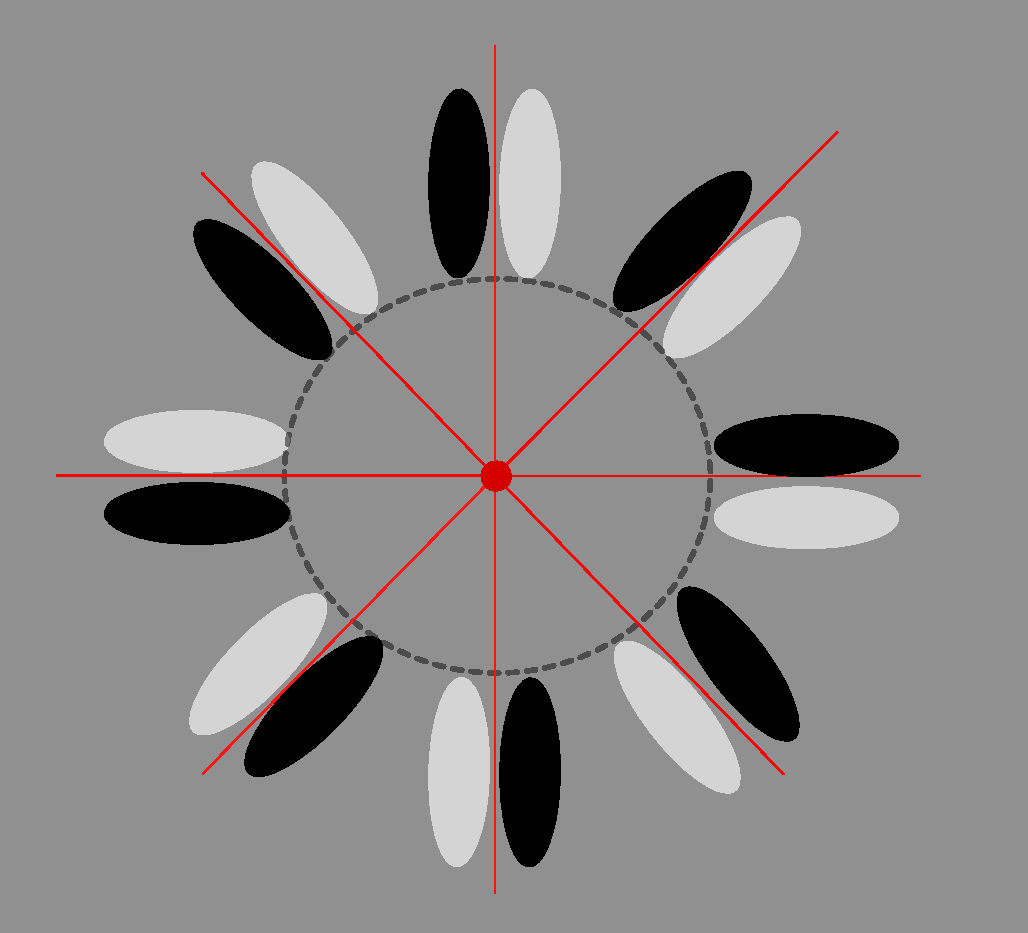
\includegraphics[width=4.5cm]{gfx/Chapter05/OrientedGabors.pdf}
\caption{This depiction of simple-cell receptive field (RF) model for V1 responses that captures only spatial -- rather than temporal -- properties in the plane of a captured image, illustrated here for a small patch of pixels. White areas indicate zones where a bright stimulus induces increased firing rate in a single neuron, dark areas represent inhibition of firing, and grey areas have null effect.  Note that the centres of the 8 RFs shown here are actually centered at the origin of local image space (indicated by the red circle) in the first layer of the CNN.  In a {\em second layer}, information is collected from different regions of the local patch and represented as a population code associated with the centre of the circle.}
\label{fig:OG}
\end{center}
\end{figure}

The second level of the convolutional network groups the orientation-selective outputs of the first level of convolution over different regions of a local image patch. It is obtained by applying a \textit{permuted tensor convolution} between $\tens{G}(\sigma,\lambda)$ and a \textit{pooling tensor} $\tens{P}$:  
\begin{equation}
\tens{D} \triangleq \tens{G}(\sigma,\lambda) \, 
   \underset{\lbrace i_3 \rbrace}{\overset{\lbrace i_1,i_2\rbrace}{[ \ast ]}}\, {\tens{P}}
\end{equation}
The pooling tensor is also an order 3 tensor that defines 17 pooling regions with respect to each location in image space, distributed in a radial and angular fashion across a patch; the values in this tensor are visualised over a normalized neighbourhood of unit width and height in Figure~\ref{fig:PoolingTensor}. The resulting order 5 tensor, $\tens{D}$, is of dimension $I_1\times I_2 \times 8 \times 17 \times N_F$. Because the slices of this tensor create different pooling regions over a patch, it is distinctly different to the pooling operations of standard CNNs, which typically use a single fixed spatial smoothing operator for each pooling layer, and not multiple poolers for which weights are learned. 

In the notation used until Section \ref{sec:tensornotation}, tensor $\tens{D}$ was used to generate the SF-GABOR descriptor, by sampling $\tens{D}$ every 3 pixels along modes $i_1$ and $i_2$, generating around 2,000 descriptor vectors per frame, each of 136 elements.

\begin{figure}[!t]
\centering
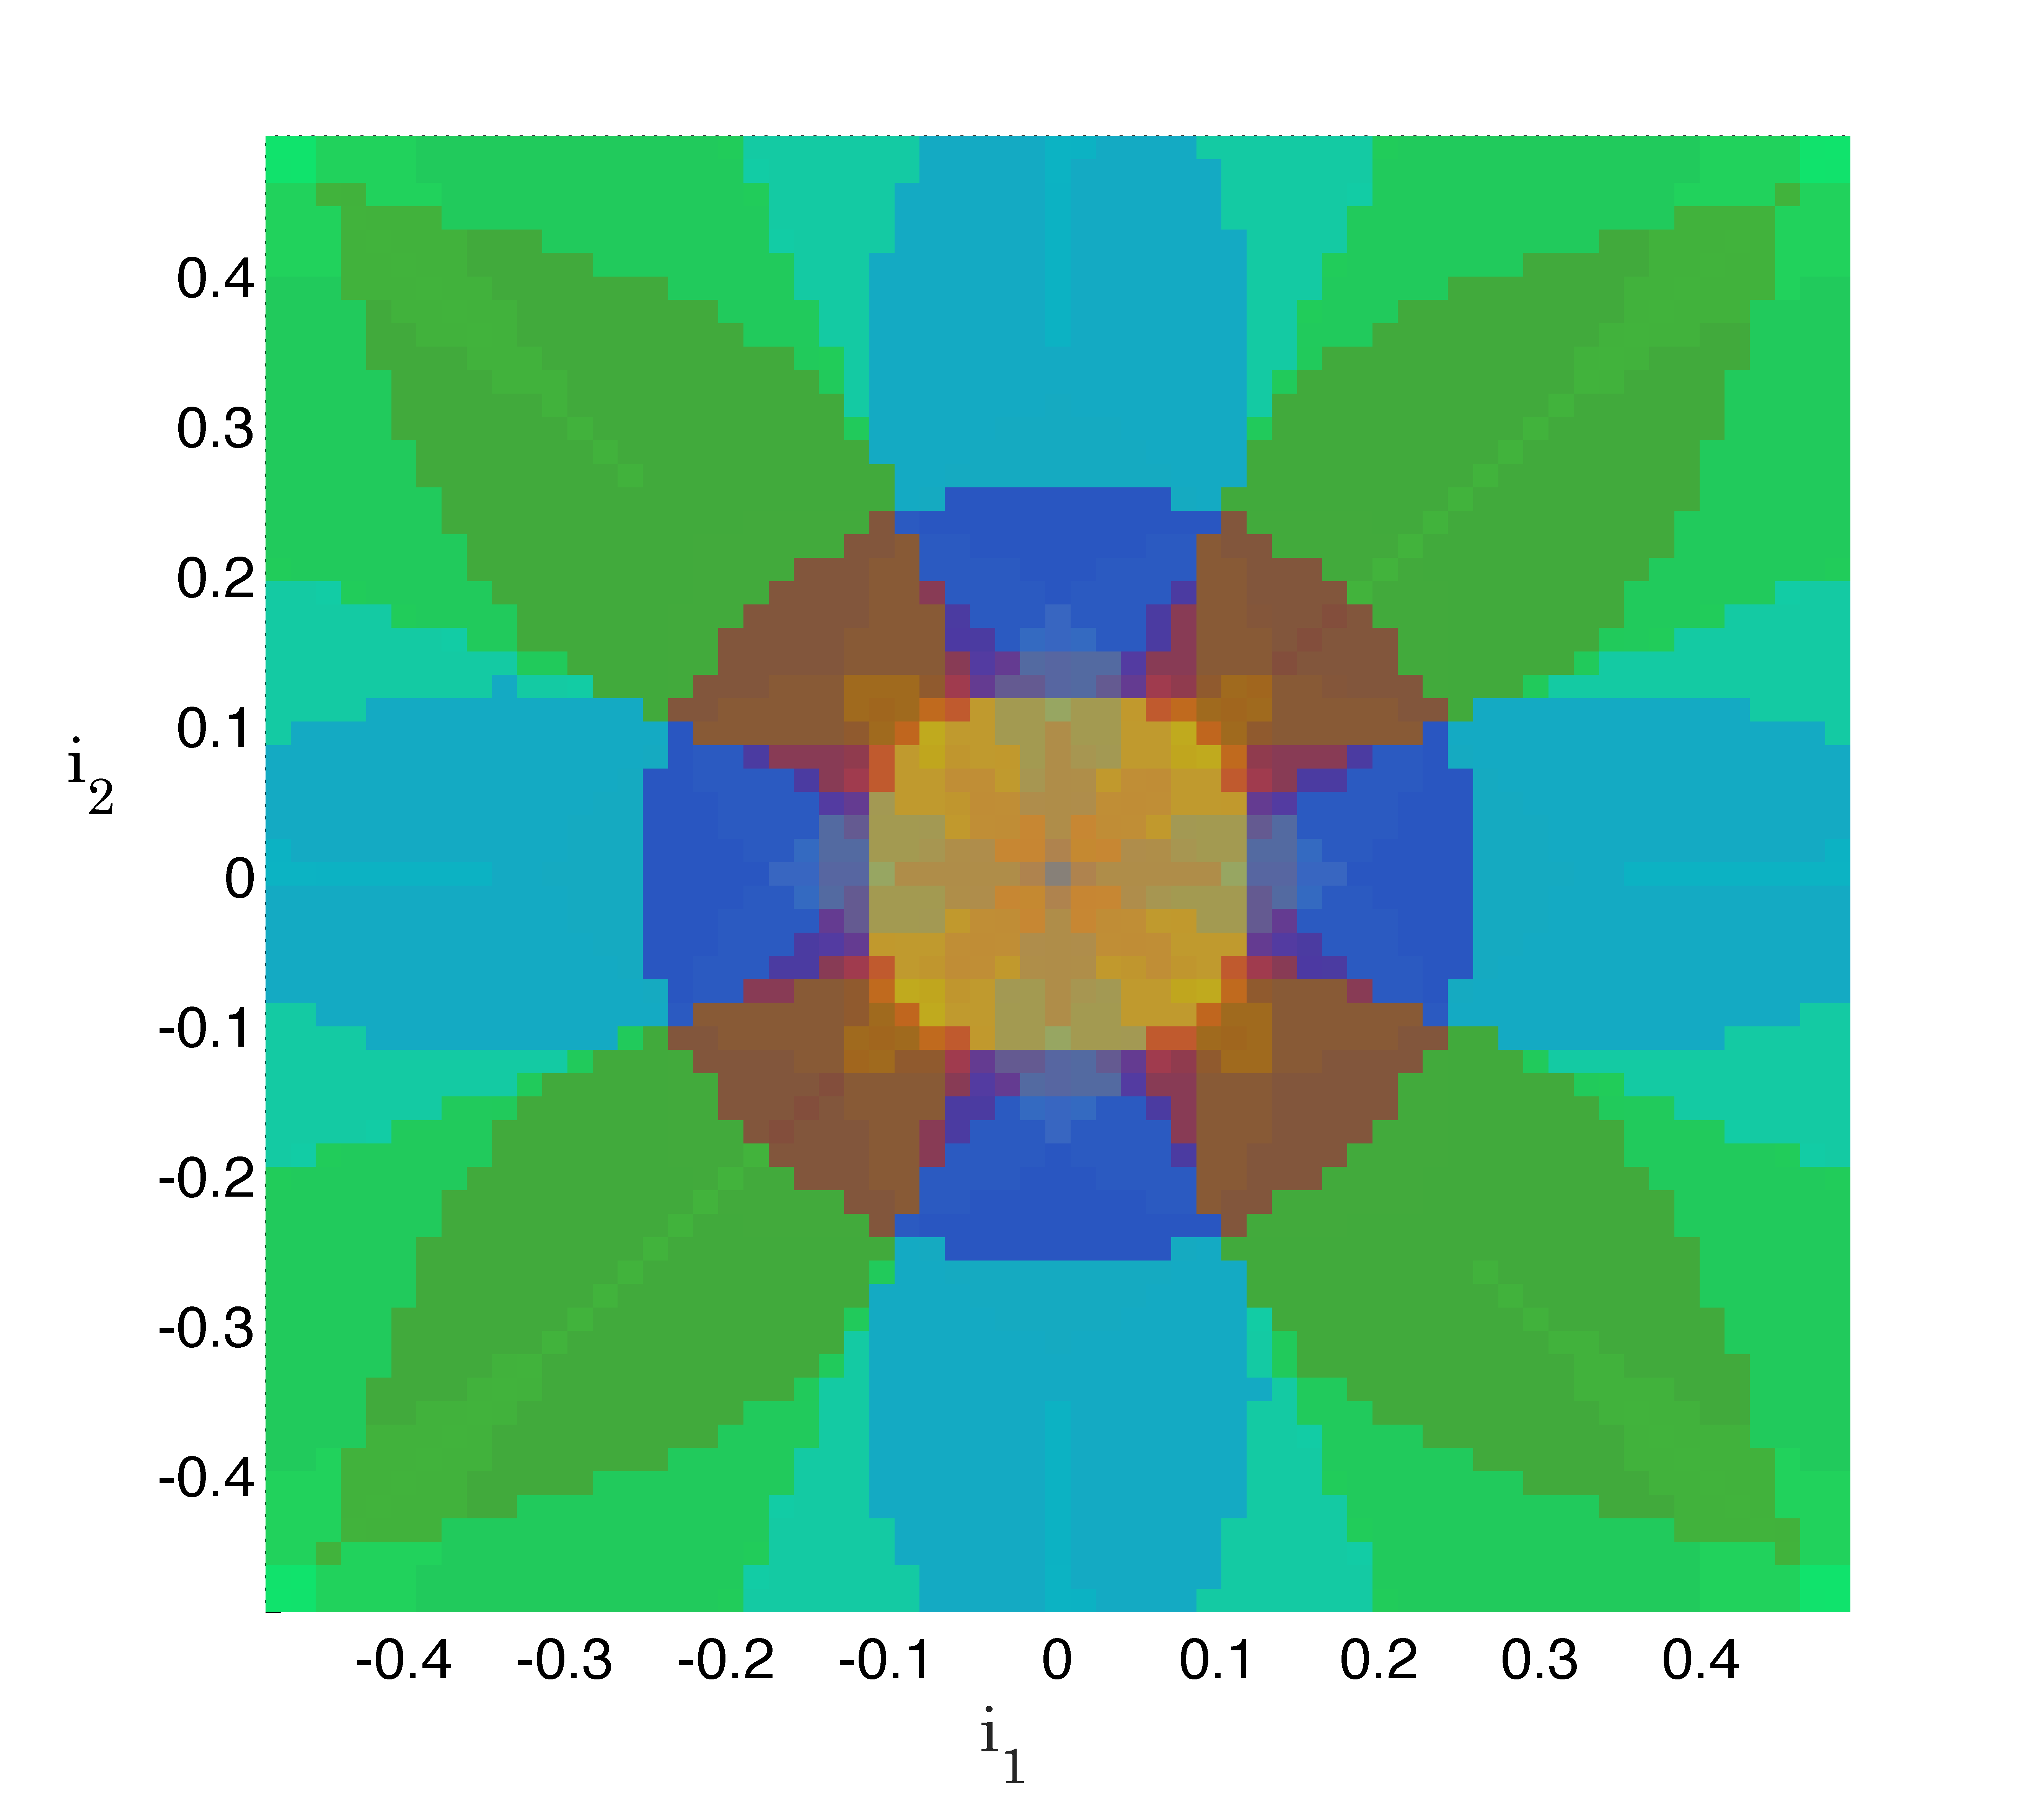
\includegraphics[width=3.5in]{gfx/Chapter05/PoolingTensorRender.png}
\caption{Illustration of the order 3 pooling tensor, visualised using transparency and colours to depict the spatial arrangement of values in the third mode. }
\label{fig:PoolingTensor}
\end{figure}


%\begin{figure}[!h]
%\begin{center}
%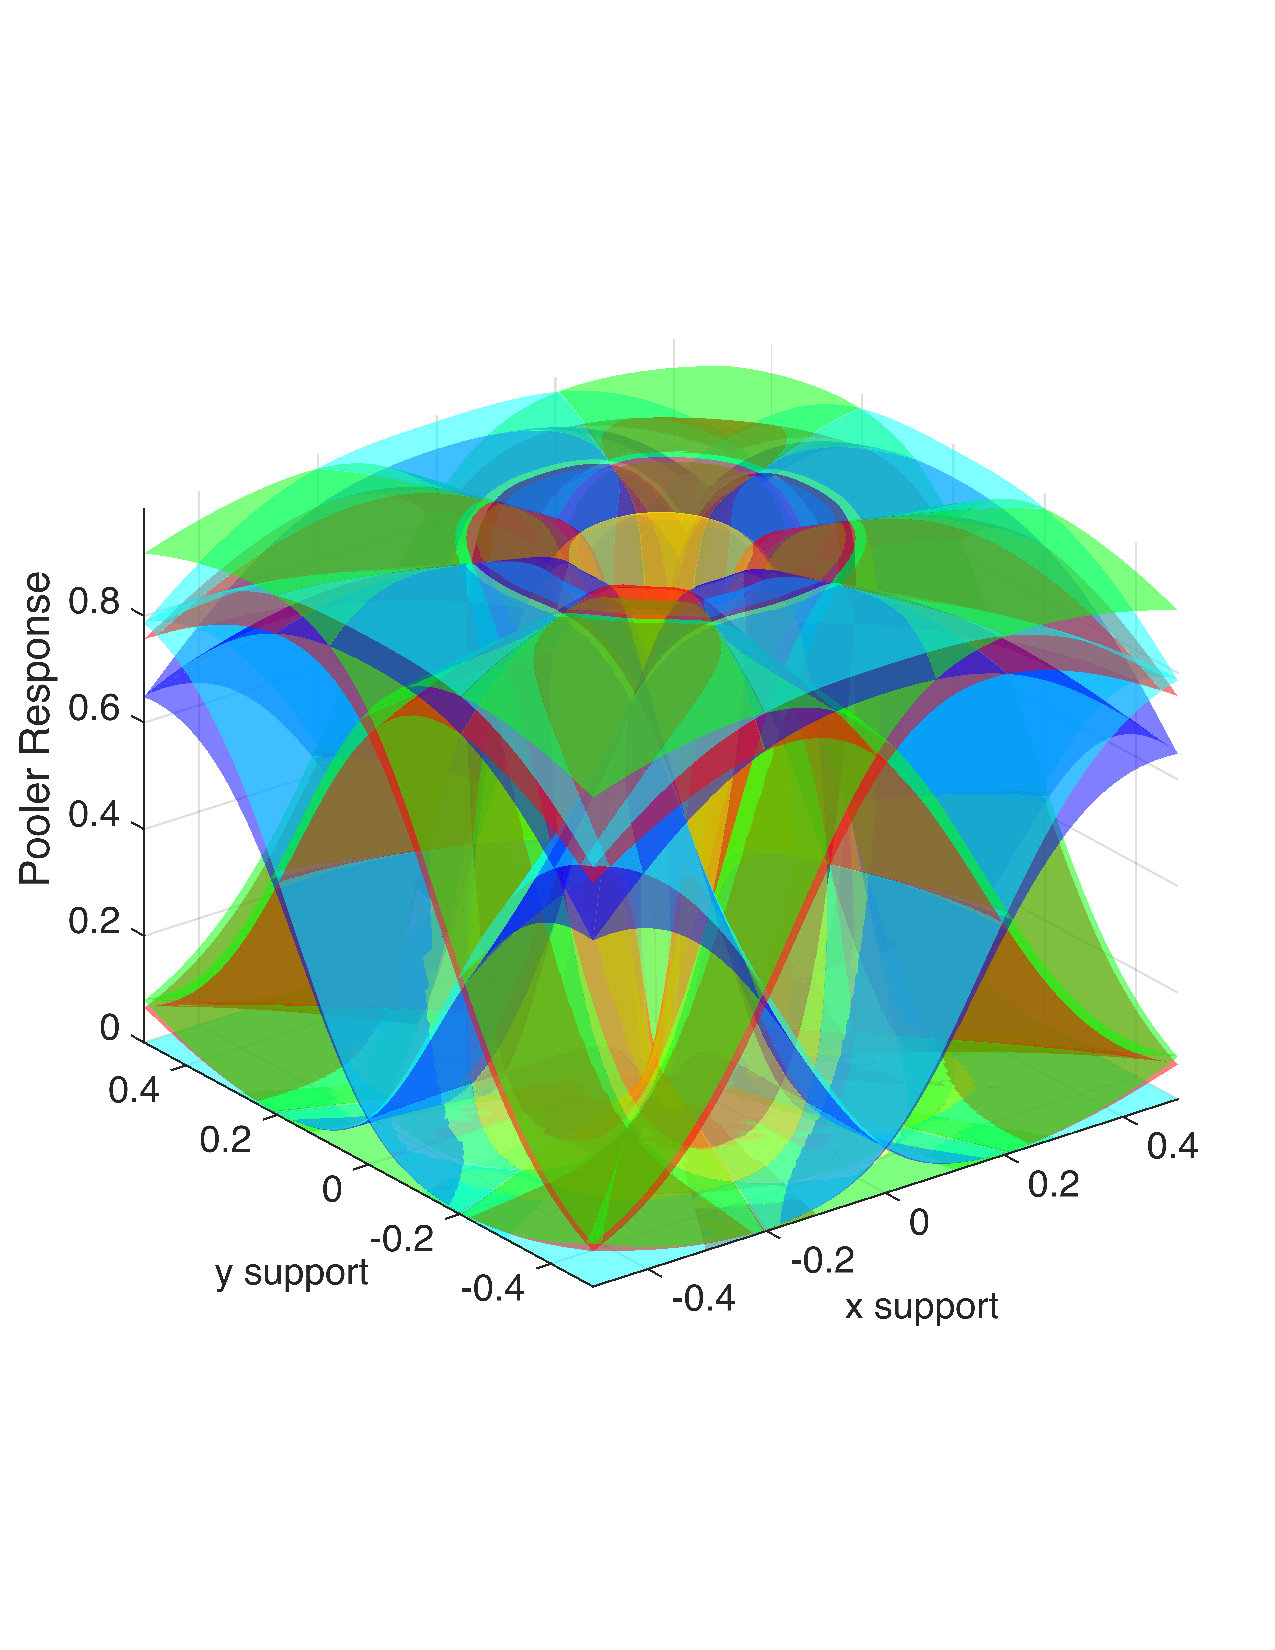
\includegraphics[width=10cm,trim=0cm 3cm 0cm 3cm,clip=true]{gfx/Chapter06/PoolerResponses.pdf}
%\caption{\label{fig:PoolerResponses3D}Patterns of 17 spatial poolers consist of regions in a centre-surround organisation, with angular variation.  These pooling weights were optimised on the PASCAL VOC 2007 dataset for categorization by an optimization approach. Colours are chosen to alternate in order to allow spatial relationships to be visible to the reader.}
%\end{center}
%\end{figure}
%%
%The response field was subsampled to yield approximately 2000 descriptors per frame, each of 136 elements.

\subsection{Subsampling}
Since the poolers are designed to be spatially smoothing, the subsampling operation can be applied directly to dimensions $i_1$ and $i_2$ of $\tens{D}$. This maintains $\tens{D}$ as an order 5 tensor, but reduces the dimensions over the two modes representing in-plane spatial location. 


\subsection{Learning CNN Weights}
Even with the use of weight-sharing, deep convolutional networks require learning anywhere of the order of millions to tens of millions of parameters. In contrast, the two-layer network described above, which uses functional spatial forms for the spatial weights layers required learning a much smaller number of parameters.  Weight learning was performed by optimising over the Gabor parameters of wavelength and spatial scale, and the pooling parameters used in the second layer of permuted convolution.

Both the pooling patterns and the Gabor parameters $\sigma$ and $\lambda$ were optimized on the PASCAL VOC 2007 database \cite{everingham2010pascal} in order to achieve good discrimination between classes of the Pascal visual database. The optimization used the criterion of Area-Under-Curve metric in an image retrieval task within the labelled image database, i.e. given a query image from a set of data, find the nearest match in a database.  Both training and testing images were taken from a partitioning of the PASCAL VOC database, and performance was measured in separate test sets.  Stochastic Gradient Descent was used. In addition, the weight set was constrained so as to sum to zero at each point in space across all convolution filters, and were constrained to be spatially antisymmetric about one axis.  No further optimizations were applied to the two early layers of the CNN once this optimisation had been done, and the optimization did not use any of the images we describe in experiments in Section~\ref{sec:experiments}.

The architecture of the CNN and the order of tensors used to represent the data flowing through it is shown in Figure~\ref{fig:arch}.

\begin{figure}
\centering
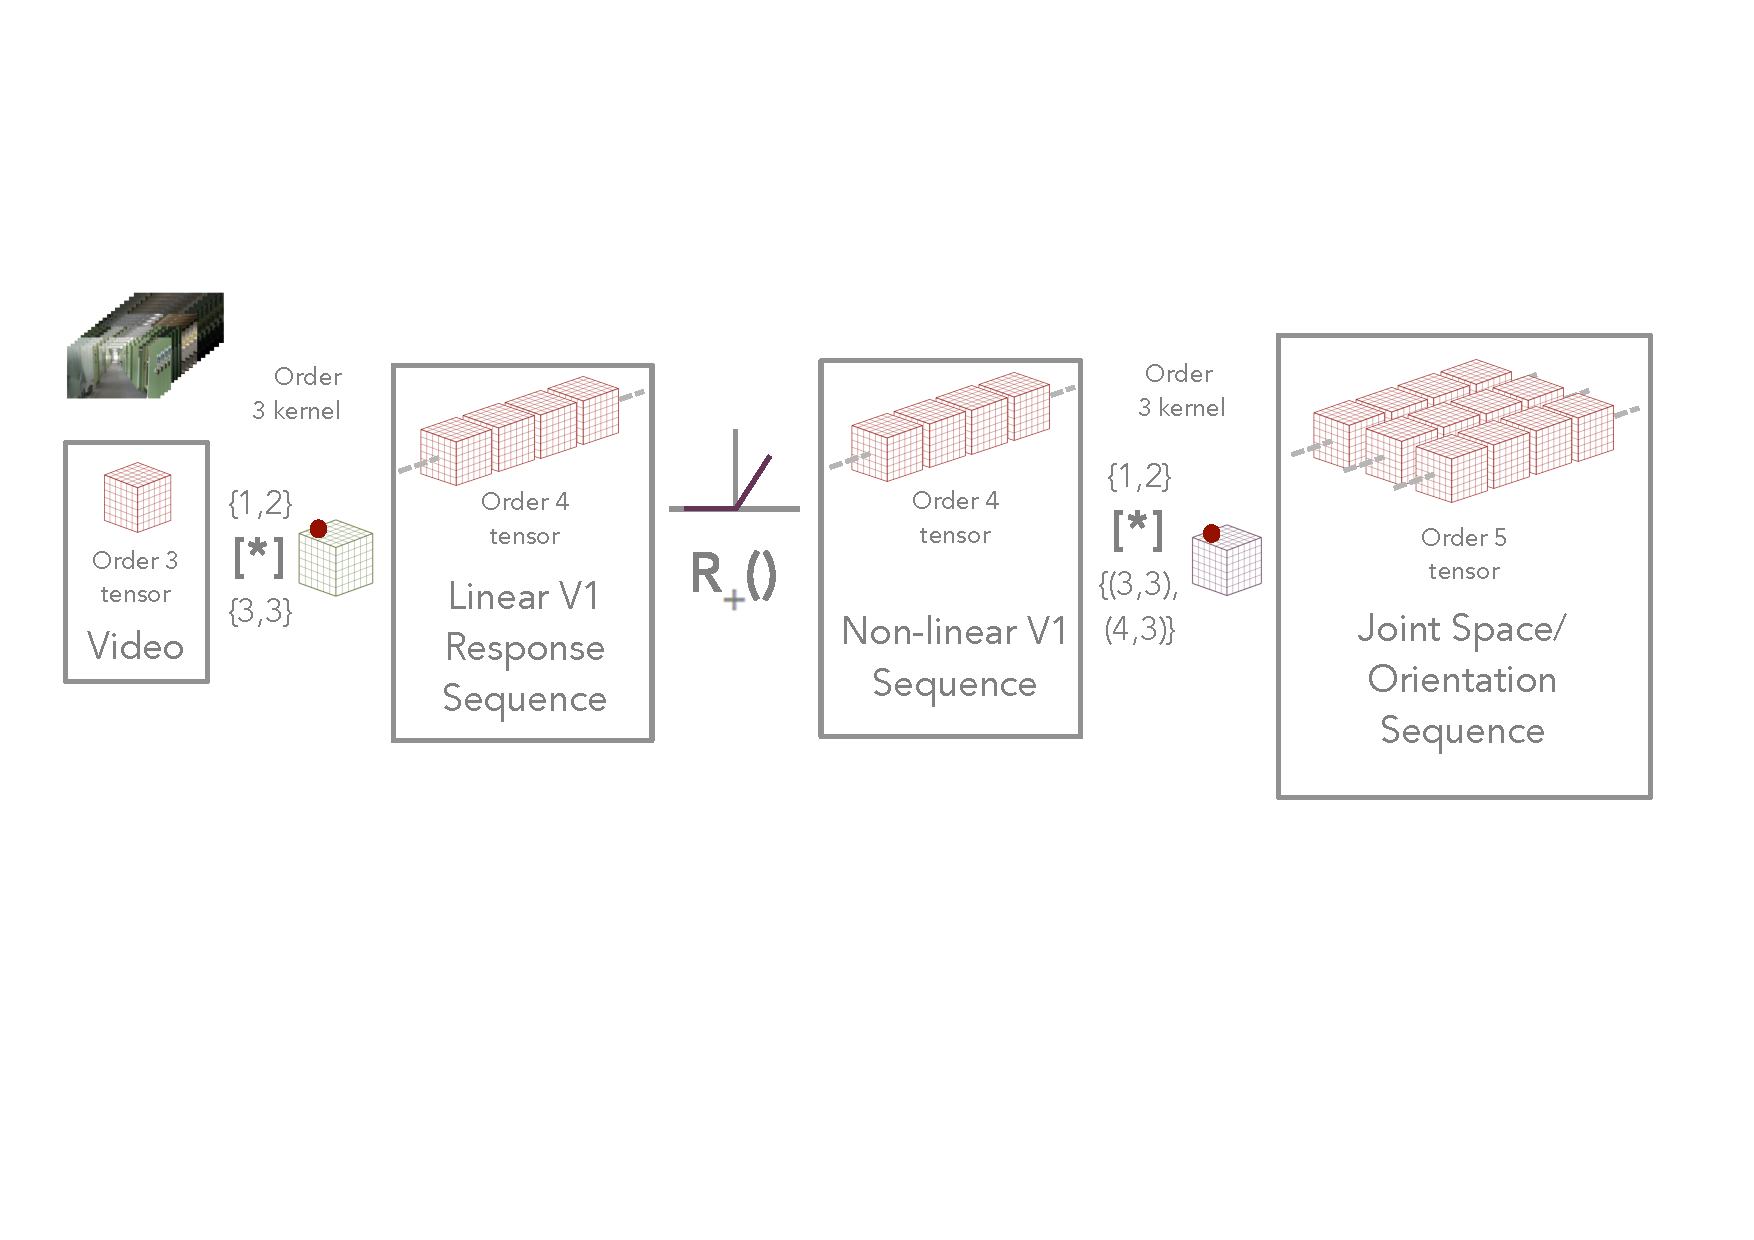
\includegraphics[width=1.1\linewidth,trim={0 7cm 0 3cm},clip]{gfx/Chapter05/video_encoding_pipeline.pdf}
\caption{Illustration of the CNN that simulates simple-cell responses and a population code based on neurons in visual area V1 applied to a video sequence captured from a wearable or hand-held camera.  In terms of biological complexity, this is quite a crude model: does not include strong non-linearities such as divisive normalisation of phase quadrature
responses \cite{petrou2008next}. Nevertheless, it captures the behaviour of a significant subset of biological cell responses in area V1 \cite{carandini1997predictions}. Sub-sampling in modes $(i_1,i_2)$ is omitted for clarity.}
\label{fig:arch}
\end{figure}

\subsection{Dictionary Encoding}
The convolutional network to produce a joint encoding of orientation and spatial position within a patch yields an order 5 tensor once applied to an intensity-only video sequence.  Consider two order 5 tensors, $\tens{A}$ and $\tens{B}$, each of which represents an encoding of a video-sequence.  One of these, $\tens{A}$, will be treated as modelling a simple V1 population code in a sequence captured during a journey; the other, $\tens{B}$ is treated as a visual memory of a previous journey.  Searching this order 5-space for particular patterns is difficult: for a wide-angle input video of size around $240\times120$ pixels, for example, an order 4 tensor (corresponding to one time-point) contains around 272,000 elements.  The first two modes of $\tens{A}$ and $\tens{B}$ correspond to location in the image plane; the next two dimensions provide the population code over a patch of pixel data, and the final mode corresponds to time.  


One solution to the search problem is to apply vector quantization to some of the dimensions.  For example, by treating three of the five dimensions ($i_1,i_2,i_5$) as observations of variables across the remaining two dimensions $(i_3,i_4)$, a dictionary, $\mathcal{V}$ can be constructed; an encoding of a single frame using this dictionary can then be achieved using an order 2 tensor.  This reduces the frame comparison problem to one that is performed by comparing dictionary encodings. The dictionary encoding acts as a simple technique for dimensionality reduction, but it allows a more efficient comparison between a visual memory and a new visual stimulus within the modelled population code. We used the $k-$means algorithm because of its simplicity and reasonable scalability when dictionary sizes range from the order of hundreds of terms to the order of thousands.

The dictionary encoding is applied at the frame-level, so that each frame in a video sequence is represented by an order 1 tensor.  The complete sequence of frames of a journey, then, is represented by an order 2 tensor, with dimensions $N_F\times|\mathcal{V}|.$ 


\subsection{Artificial Place Cells in the tensor population model}
\label{sec:APC}

Finally, we express the artificial place cells in the tensor formulation. Given the population code for a video sequence, represented by the tensor $\tens{S}_p$, we now aim to model the behaviour of place-cells themselves.   Population codes for individual frames are represented by the occurrences with which certain patterns in modes $i_3,i_4$ are observed within a frame.   Once encoded using the dictionary $\mathcal{V}$, which contains terms $t_1,t_2,...,t_{\mathcal{V}}$, the dimensions corresponding to the joint orientation and spatial encoding over patches is collapsed to a single term for each patch, and the set of numbers over the entire frame (dimensions $i_1,i_2$) are converted into a term-frequency representation \cite{Wu:2008} (see Fig.~\ref{fig:HistEncodings}).

\begin{figure}
\centering
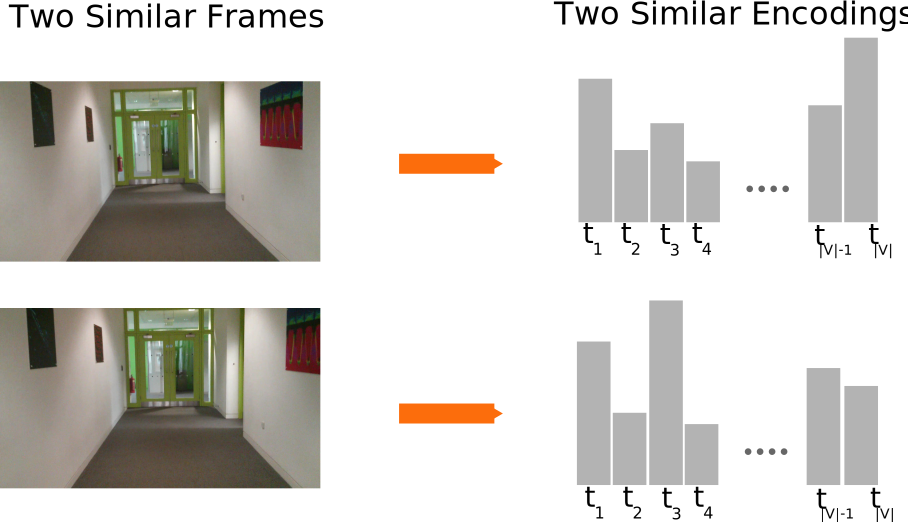
\includegraphics[width=3.5in]{gfx/Chapter05/HistogramEncodings.pdf}
\caption{Two image frames should have similar representations along the fibre in the order 2 tensor that contains an encoded image sequence.  Here, two similar frames are shown with (diagrammatic) representations taken from along the fibre corresponding to particular frames.  The elements of the fibre correspond to dictionary terms, and the occurrence of each term is recorded.  We used the $\chi^2$ similarity measure.}
\label{fig:HistEncodings}
\end{figure}


In line with the findings described in Section \ref{sec:ch5experiments}, we found that the $\chi^2$ similarity measure was an appropriate way to compare two histograms. That is, individual fibres, one a single order 1 tensor $\mathbf{q}$ and a second drawn from a previously encoded sequence from a different journey, $\tens{S}_p$, yielded behaviour that decayed gently from the true location of the query shot when using the $\chi^2$ similarity measure, provided that very low similarity scores were thresholded out.  That is, due to the presence of noise, there is a threshold to the $\chi^2$ score above which place-cell like behaviour could be observed.  By varying the height at which APCs are considered to be active, the width of an APC response can be altered.  Altering APCs width is key to to methods of localization that are discussed in the next section.  



\section{Conclusion}

Place cell physiology and function is of immense interest for a number of reasons. To our knowledge, there is no computational architecture that reproduces place-cell responses in the form of tuning curves artificially from video sequences, and there is no biologically plausible model for place cell encoding that can be applied to the recorded video sequences we have used in this work.  Furthermore, competing camera-based localization techniques such as SLAM rely on relative object camera motion to infer structure and to then either perform odometry or to estimate location: motion is a requirement.  The place cell model we propose and evaluated in this chapter does not require motion at location estimation time: a single frame gives a possible response.

A number of questions observed from this study motivates further work in the search of a plausible biological answer. First, it is the nature of the place cells what defines their width after thresholding, and thus their sensitivity to locations. In biology, neurons are known to reach a certain threshold potential before they fire an action potential or impulse that can propagate along the axon and eventually trigger similar responses on other cells. We are planning to study this effect and extend the model of the place cell by also incorporating a model of its firing that takes into account the shape of the firing envelope and the causes of the activity.


Perhaps a greater problem, from a biological perspective, is that it is unclear how grid cells might fit into the model we have proposed in this chapter.  One intriguing prediction is that grid cells are implicit in the existence of place cells; in other words, place cells are not entirely formed from grid cells, but working place cells create a grid-like pattern of activation if one grid cell is wired to several spaced place cells.  This observation may be related to observed loop-like connectivity observed between hippocampus and entorhinal cortex. 

In third place, we have found that the best performing methods are SF-GABOR and SIFT (sparse and dense). This poses another question worth investigating and is that of the relationship of better performance with the closeness of the local patch description method with models of early vision. It is known that the 2D Gabor filters in SF/ST-GABOR descriptors present the orientation-selective simple cell receptive fields behavior of the primary visual cortex (V1). Similarly, the difference of Gaussians (DoG) space representation found in Lowe's SIFT keypoint detection may be seen as an approximation of the spatial receptive field of a retinal ganglion cell. Lowe also suggested that the process behind the computation of the orientation of the frequencies is similar to the behavior of complex cells in V1.


In conclusion, the work described in this chapter demonstrates that computational models of place cells can provide effective estimates of camera location without relying on tracking or construction of a geometric model of the local environment. To our knowledge, there has been no reported computational architecture that reproduces biological place cell responses in the form of tuning curves from video sequences, and there have been no other demonstrable computational models for place cell positional encoding that can be applied to the recorded video sequences of the form we used in this work.  Furthermore, competing camera-based localisation techniques such as SLAM rely on relative object camera motion to infer structure and to then either perform odometry or to estimate position: motion is therefore a requirement.  The place cell model that we have proposed and evaluated in this chapter does not require motion at location estimation time: a single frame yields a hypothetical location.


%*****************************************
%*****************************************
%*****************************************
%*****************************************
%*****************************************